\documentclass[a4paper,DIV=12,11pt,parskip=half]{scrartcl}
\usepackage{fontspec}
\usepackage{graphicx}
\usepackage{fancyhdr}
\usepackage{times}
\usepackage{tabularx}
\usepackage{ltablex}
\usepackage{color,colortbl}
\usepackage[bookmarks,colorlinks,linkcolor=blue]{hyperref}
\usepackage{listings}
\usepackage{makeidx}
\usepackage{alltt}
\usepackage{upquote}
\usepackage{verbatim}
\usepackage[numbered, open, openlevel=2]{bookmark}
\usepackage{caption}
\usepackage{everyshi}
\usepackage{lmodern}
\usepackage{nameref}
\usepackage{fancybox,color}
\usepackage{epic}
% nice picture \oval (corners fit straight lines)
\usepackage{pict2e}
\usepackage{boxedminipage}
\usepackage{float}
%
\addtolength{\textheight}{2cm}
\definecolor{SteelBlue}     {rgb}{0.27,0.51,0.71}
\definecolor{DarkGreen}     {rgb}{0.0, 0.5, 0.0}
\definecolor{DarkRed}       {rgb}{0.8, 0.0, 0.0}

\newcommand{\structure}[1]{\textcolor{SteelBlue}{\bfseries #1}}

\newcommand{\Intens}[1][ ]{\textcolor{SteelBlue}{\bfseries INTENS}#1}
\newcommand{\nothing}{\rule{0pt}{0pt}}
\newcommand{\Zitat}[1]{\flqq{#1}\frqq}
\newcommand{\Slanted}[1]{{\normalfont\slshape #1}}
\newcommand{\SlantedB}[1]{{\normalfont\bfseries\slshape #1}}
\newcommand{\Bold}[1]{{\bfseries{#1}}}
\newcommand{\BoldIt}[1]{{\bfseries\textit{#1}}}
\newcommand{\BoldTt}[1]{{\bfseries\ttfamily{#1}}}
\newcommand{\Tt}[1]{{\ttfamily{#1}}}
\newcommand{\Kopffreiheit}[1][2.5ex]{\rule{0pt}{#1}}
\newcommand{\Fussfreiheit}[1][-0.7ex]{\rule[#1]{0pt}{1ex}}
\newcommand{\Tilde}{\raisebox{-0.8ex}{\~\ }}
\newcommand{\TildeTt}{\raisebox{-0.8ex}{\~\ \hspace{-0.7em}}}

\definecolor{delim}{RGB}{20,105,176}

\lstdefinelanguage{json}{
    showspaces=false,
    showtabs=false,
    breaklines=true,
    postbreak=\raisebox{0ex}[0ex][0ex]{\ensuremath{\color{gray}\hookrightarrow\space}},
    breakatwhitespace=true,
    basicstyle=\ttfamily\small,
    upquote=true,
    morestring=[b]",
}

% Standard Environments
% =====================
%%ragged2e \newenvironment{Center}[1][\textwidth]
%%ragged2e {\begin{minipage}[t]{#1}\begin{center}}
%%ragged2e {\end{center}\end{minipage}}

\newenvironment{JustLeft}[1][\textwidth]
{\begin{minipage}[t]{#1}\begin{flushleft}}
{\end{flushleft}\end{minipage}}

\newenvironment{JustRight}[1][\textwidth]
{\begin{minipage}[t]{#1}\begin{flushright}}
{\end{flushright}\end{minipage}}

% Enumerations
% ============
\usepackage{enumitem}

\newenvironment{ItemizeBullet}[1][]
{\begin{itemize}[label=\textbullet
                ,leftmargin=1.6em
                ,#1]}
{\end{itemize}}

\newenvironment{ItemizeSquare}[1][]
{\begin{itemize}[label=\rule{1ex}{1ex}\hspace{3pt}
                ,leftmargin=1.6em
                ,#1]}
{\end{itemize}}

\newenvironment{ItemizeDash}[1][]
{\begin{itemize}[label=\textendash
                ,leftmargin=1.6em
                ,#1]}
{\end{itemize}}

\newenvironment{EnumAlpha}[1][]
{\begin{enumerate}[label=\alph*)
                ,leftmargin=1.8em
                ,#1]}
{\end{enumerate}}

\newenvironment{EnumArabic}[1][]
{\begin{enumerate}[label=\arabic*.
                  ,leftmargin=1.8em
                  ,#1]}
{\end{enumerate}}

\newenvironment{CompactItemBullet}[1][]
{\begin{itemize}[label=\textbullet
                ,topsep=0pt
                ,partopsep=\parsep
                ,parsep=0pt
                ,itemsep=0pt
                ,leftmargin=1.8em
                ,labelwidth=1em
                ,#1]}
{\end{itemize}}

\newenvironment{CompactItemDash}[1][]
{\begin{itemize}[label=\textendash
                ,topsep=0pt
                ,partopsep=\parsep
                ,parsep=0pt
                ,itemsep=0pt
                ,leftmargin=1.8em,labelwidth=1em
                ,#1]}
{\end{itemize}}

\newenvironment{CompactItemSquare}[1][]
{\begin{itemize}[label=\raisebox{0.3ex}{\rule{0.8ex}{0.8ex}}\hspace{2pt}
                ,topsep=0pt
                ,partopsep=\parsep
                ,parsep=0pt
                ,itemsep=2pt
                ,leftmargin=1.6em
                ,labelwidth=1em
                ,#1]}
{\end{itemize}}

\newenvironment{CompactEnumAlpha}[1][]
{\begin{enumerate}[label=\small\alph*)
                  ,leftmargin=1.8em
                  ,topsep=0pt
                  ,partopsep=\parsep
                  ,parsep=0pt
                  ,itemsep=0pt
                  ,leftmargin=1.6em
                  ,labelwidth=1em
                  ,#1]}
{\end{enumerate}}

% Directory Tree
% ==============
\usepackage{dirtree}

\renewcommand*\DTstyle{\ttfamily}
\renewcommand*\DTstylecomment{\color{DarkGreen}\rmfamily\small}
\DTsetlength{0.2em}{1em}{0.2em}{0.4pt}{3pt}

\newcommand{\DirectoryTree}[1]{
\begin{JustLeft}[\linewidth]
\renewcommand{\dotfill}{\leaders\hbox to 12pt{\hss.\hss}\hfill}
\dirtree{#1}
\end{JustLeft}\\%
}

% Boxes
% =====
\usepackage{tcolorbox}

\newenvironment{WhiteBox}[1][]
{\begin{tcolorbox}
  [colback=white
  ,arc=0pt
  ,boxrule=1pt
  ,boxsep=0pt
  ]%
}
{\end{tcolorbox}}

\newenvironment{Note}[1][]
{\begin{tcolorbox}
  [colback=yellow!20!white
  ,colframe=black
  ,colbacktitle=red!50!white
  ,coltitle=black
  ,fonttitle=\bfseries
  ,title=\Kopffreiheit Note \Fussfreiheit
  ,arc=0pt
  ,boxrule=1pt
  ,boxsep=0pt
  ,center
  ,#1
  ]}
{\end{tcolorbox}}

\lstset{%
  basicstyle=\small,
  keywordstyle=\color{blue}\bfseries\sffamily,
  identifierstyle=\ttfamily,
  commentstyle=\em,
  stringstyle=\ttfamily,
  extendedchars=true,
  showstringspaces=false,
  literate=%
   {Ω}{{O}}1
{Ö}{{\"O}}1
{Ä}{{\"A}}1
{Ü}{{\"U}}1
{ß}{{\ss}}2
{ü}{{\"u}}1
{ä}{{\"a}}1
{ö}{{\"o}}1
}
\lstdefinestyle{DescStyle}{%
  basicstyle=\footnotesize,
  frame=single,
  backgroundcolor=\color{yellow!5!white},
  keywordstyle=\color{blue},
  identifierstyle=\ttfamily,
  commentstyle=\em,
  stringstyle=\ttfamily,
  extendedchars=true,
  showstringspaces=false,
  escapechar=\£,
  morekeywords={*,INTEGER,REAL,STRING,EDITABLE,SCALAR,LABEL,HELPTEXT,UNIT,DBUNIT,PERSISTENT
               ,FIELDGROUP,DATAPOOL,END,STRUCT,BUTTON,FUNC,UI_MANAGER,PLOT2D,FORM
               ,FUNCTIONS,MAP,VOID,COLSPAN,STREAMER,OPERATOR,PROCESS,PROCESSGROUP
               ,DISPLAY,NONE,HIDDEN,SILENT,NO_LOG,JSON,BATCH,MATLAB,FOLDER,MAIN
               ,YAXIS1,YAXIS2,MESSAGE_QUEUE,REQUEST,HOST,RESOURCE,PORT_REQUEST,TIMEOUT
               ,TASK,HEADER,RESPONSE,MESSAGEBOX,ABORT},
}

\lstdefinestyle{CmdStyle}{%
  basicstyle=\footnotesize,
  frame=single,
  backgroundcolor=\color{blue!8!white},
  escapechar=\£
}

\lstdefinestyle{ShellStyle}{%
  basicstyle=\footnotesize,
  frame=single,
  backgroundcolor=\color{blue!15!white},
  escapechar=\£
}

\lstdefinestyle{URLStyle}{%
  basicstyle=\small,
  frame=single,
  backgroundcolor=\color{red!10!white},
  escapechar=\£
}

\lstdefinestyle{PyStyle}{%
  basicstyle=\footnotesize,
  frame=single,
  backgroundcolor=\color{green!10!white},
  escapechar=\£
}

\lstdefinestyle{ListStyle}{%
  basicstyle=\footnotesize,
  frame=single,
  backgroundcolor=\color{white},
  escapechar=\£
}

\lstdefinestyle{DockerStyle}{%
  basicstyle=\footnotesize,
  frame=single,
  backgroundcolor=\color{magenta!20!white},
  escapechar=\£,
  keywordstyle=\color{black}\bfseries\sffamily,
  morekeywords={*,MAINTAINER,FROM,LABEL,RUN,ADD,COPY,ENV,EXPOSE,ENTRYPOINT,CMD},
  numbers=left,
  stepnumber=1,
  numberstyle=\tiny,
  numbersep=2ex,
}

\lstdefinestyle{ComposeStyle}{%
  basicstyle=\footnotesize,
  frame=single,
  backgroundcolor=\color{green!20!white},
  escapechar=\£,
  keywordstyle=\color{blue}\bfseries\sffamily,
  morekeywords={*,version,services,image,build,command,deploy,replicas,placement,constraints,
                ports,volumes,depends_on,environment,networks},
  numbers=left,
  stepnumber=1,
  numberstyle=\tiny,
  numbersep=2ex,
}

\newcommand{\strich}{\ttfamily\textminus}

\newcolumntype{A}{%
  >{\color{white}\columncolor[gray]{.8}}c
}

\defaultfontfeatures{Ligatures={TeX}}
%\setsansfont{CMU Sans Serif}%{Arial}
%\setmainfont{CMU Serif}%{Times New Roman}
%\setmonofont{CMU Typewriter Text}%{Consolas}
\keepXColumns

% Index
% indexheading is used in sysadmin.mst
\newcommand{\indexheading}[1]{%
\hypertarget{index:#1}{\centerline{\Large{#1}}\nopagebreak}%
\pdfbookmark[2]{#1}{index:#1}
}%
\makeindex
\usepackage[totoc]{idxlayout}
%
% top align includegraphics
\usepackage[export]{adjustbox}
\usepackage{listings} % lstlisting

\raggedbottom

\usepackage[strict]{changepage}
%% to print some pages in one
%% \usepackage{lscape}
%
% This is the layout command
\newcommand{\keyword}[1]{\mbox{\bfseries\sffamily {#1}}}
%
% here are all INTENS keywords
%
\def\ABORT{\keyword{ABORT}}
\def\ABORTTRANSACTION{\keyword{ABORTTRANSACTION}}
\def\ABS{\keyword{ABS}}
\def\ACOS{\keyword{ACOS}}
\def\AFTERDBLOGON{\keyword{AFTER\_DB\_LOGON}}
\def\AFTERUPDATEFORMS{\keyword{AFTER\_UPDATE\_FORMS}}
\def\ALARMCOLOR{\keyword{ALARM\_COLOR}}
\def\ALARMLEVEL{\keyword{ALARM\_LEVEL}}
\def\ALIGN{\keyword{ALIGN}}
\def\ALLCYCLES{\keyword{ALLCYCLES}}
\def\ALLOW{\keyword{ALLOW}}
\def\ALWAYS{\keyword{ALWAYS}}
\def\APPEND{\keyword{APPEND}}
\def\APPMODAL{\keyword{APP\_MODAL}}
\def\ANNOTATION{\keyword{ANNOTATION}}
\def\AREA{\keyword{AREA}}
\def\ARG{\keyword{ARG}}
\def\ARROWS{\keyword{ARROWS}}
\def\AS{\keyword{AS}}
\def\ASCII{\keyword{ASCII}}
\def\ASIN{\keyword{ASIN}}
\def\ASPECTRATIO{\keyword{ASPECT\_RATIO}}
\def\ASPECTRATIOREFAXIS{\keyword{ASPECT\_RATIO\_REF\_AXIS}}
\def\ASSIGNCONSISTENCY{\keyword{ASSIGN\_CONSISTENCY}}
\def\ASSIGNCORR{\keyword{ASSIGN\_CORR}}
\def\ATAN{\keyword{ATAN}}
\def\ATANTWO{\keyword{ATAN2}}
\def\ATTRS{\keyword{ATTRS}}
\def\AUTOCLEARDEPENDENCIES{\keyword{AUTOCLEAR\_DEPENDENCIES}}
\def\AUTOLEVEL{\keyword{AUTOLEVEL}}
\def\AUTOSCROLL{\keyword{AUTO\_SCROLL}}
\def\AUTOWIDTH{\keyword{AUTO\_WIDTH}}
\def\AVG{\keyword{AVG}}
\def\AXESORIGIN{\keyword{AXES\_ORIGIN}}
\def\AXESORIGINX{\keyword{AXES\_ORIGIN\_X}}
\def\AXESORIGINY{\keyword{AXES\_ORIGIN\_Y}}

\def\BAR{\keyword{BAR}}
\def\BASE{\keyword{BASE}}
\def\BASENAME{\keyword{BASENAME}}
\def\BATCH{\keyword{BATCH}}
\def\BEEP{\keyword{BEEP}}
\def\BEGINTRANSACTION{\keyword{BEGINTRANSACTION}}
\def\BINARY{\keyword{BINARY}}
\def\BOTTOM{\keyword{BOTTOM}}
\def\BUTTON{\keyword{BUTTON}}
\def\BUTTONCANCEL{\keyword{BUTTON\_CANCEL}}
\def\BUTTONNO{\keyword{BUTTON\_NO}}
\def\BUTTONYES{\keyword{BUTTON\_YES}}
\def\BUTTONS{\keyword{BUTTONS}}

\def\CAPTION{\keyword{CAPTION}}
\def\CDATA{\keyword{CDATA}}
\def\CELL{\keyword{CELL}}
\def\CENTER{\keyword{CENTER}}
\def\CHANGED{\keyword{CHANGED}}
\def\CLASS{\keyword{CLASS}}
\def\CLASSNAME{\keyword{CLASSNAME}}
\def\CLEAR{\keyword{CLEAR}}
\def\CLEARCYCLE{\keyword{CLEARCYCLE}}
\def\CLEARSELECTION{\keyword{CLEAR\_SELECTION}}
\def\CLOSEBUTTON{\keyword{CLOSE\_BUTTON}}
\def\COMMITTRANSACTION{\keyword{COMMITTRANSACTION}}
\def\COL{\keyword{COL}}
\def\COLOR{\keyword{COLOR}}
\def\COLORBIT{\keyword{COLORBIT}}
\def\COLORSCALE{\keyword{COLOR\_SCALE}}
\def\COLSPAN{\keyword{COLSPAN}}
\def\COMBOBOX{\keyword{COMBOBOX}}
\def\COMPARE{\keyword{COMPARE}}
\def\COMPLEX{\keyword{COMPLEX}}
\def\COMPOSE{\keyword{COMPOSE}}
\def\COMPOSESTRING{\keyword{COMPOSE\_STRING}}
\def\CONFIRM{\keyword{CONFIRM}}
\def\CONFIRMCANCEL{\keyword{CONFIRM\_CANCEL}}
\def\CONTOUR{\keyword{CONTOUR}}
\def\COPY{\keyword{COPY}}
\def\COS{\keyword{COS}}
\def\CREATE{\keyword{CREATE}}
\def\CURRENTDATE{\keyword{CURRENT\_DATE}}
\def\CURRENTTIME{\keyword{CURRENT\_TIME}}
\def\CURRENTDATETIME{\keyword{CURRENT\_DATETIME}}
\def\CYCLE{\keyword{CYCLE}}
\def\CYCLENAME{\keyword{CYCLENAME}}

\def\DAEMON{\keyword{DAEMON}}
\def\DATA{\keyword{DATA}}
\def\DATAPOOL{\keyword{DATAPOOL}}
\def\DATASETTEXT{\keyword{DATASET\_TEXT}}
\def\DATASIZE{\keyword{DATA\_SIZE}}
\def\DATE{\keyword{DATE}}
\def\DBASSEMBLY{\keyword{DBASSEMBLY}}
\def\DBATTR{\keyword{DBATTR}}
\def\DBMANAGER{\keyword{DB\_MANAGER}}
\def\DBLIST{\keyword{DBLIST}}
\def\DBUNIT{\keyword{DBUNIT}}
\def\DEBUG{\keyword{DEBUG}}
\def\DELAY{\keyword{DELAY}}
\def\DELETE{\keyword{DELETE}}
\def\DELETECYCLE{\keyword{DELETECYCLE}}
\def\DELIMITER{\keyword{DELIMITER}}
\def\DEPENDENCIES{\keyword{DEPENDENCIES}}
\def\DESCRIPTION{\keyword{DESCRIPTION}}
\def\DESCRIPTIONFILE{\keyword{DESCRIPTION\_FILE}}
\def\DIAGRAM{\keyword{DIAGRAM}}
\def\DIAGRAMXPOS{\keyword{DIAGRAM\_XPOS}}
\def\DIAGRAMYPOS{\keyword{DIAGRAM\_YPOS}}
\def\DIRNAME{\keyword{DIRNAME}}
\def\DISABLE{\keyword{DISABLE}}
\def\DISALLOW{\keyword{DISALLOW}}
\def\DISCRETE{\keyword{DISCRETE}}
\def\DISPLAY{\keyword{DISPLAY}}
\def\DOTS{\keyword{DOTS}}
\def\DROP{\keyword{DROP}}

\def\EDITABLE{\keyword{EDITABLE}}
\def\ELSE{\keyword{ELSE}}
\def\ENABLE{\keyword{ENABLE}}
\def\END{\keyword{END}}
\def\EOLN{\keyword{EOLN}}
\def\ERASE{\keyword{ERASE}}
\def\ERROR{\keyword{ERROR}}
\def\EXIT{\keyword{EXIT}}
\def\EXPAND{\keyword{EXPAND}}
\def\EXPLICIT{\keyword{EXPLICIT}}
\def\EXTENSION{\keyword{EXTENSION}}

\def\FALSE{\keyword{FALSE}}
\def\FATAL{\keyword{FATAL}}
\def\FIELDGROUP{\keyword{FIELDGROUP}}
\def\FILE{\keyword{FILE}}
\def\FILENAME{\keyword{FILENAME}}
\def\FILESTREAM{\keyword{FILESTREAM}}
\def\FILTER{\keyword{FILTER}}
\def\FIRSTCYCLE{\keyword{FIRSTCYCLE}}
\def\FIRSTLEVEL{\keyword{FIRSTLEVEL}}
\def\FOLDER{\keyword{FOLDER}}
\def\FORM{\keyword{FORM}}
\def\FORMAT{\keyword{FORMAT}}
\def\FORTRAN{\keyword{FORTRAN}}
\def\FRAME{\keyword{FRAME}}
\def\FROM{\keyword{FROM}}
\def\FROMSTRINGDATETIME{\keyword{FROM\_STRING\_DATETIME}}
\def\FUNC{\keyword{FUNC}}
\def\FUNCTION{\keyword{FUNCTION}}
\def\FUNCTIONS{\keyword{FUNCTIONS}}

\def\GET{\keyword{GET}}
\def\GETCYCLE{\keyword{GETCYCLE}}
\def\GETSELECTION{\keyword{GET\_SELECTION}}
\def\GETSORTCRITERIA{\keyword{GET\_SORT\_CRITERIA}}
\def\GETTEXT{\keyword{GETTEXT}}
\def\GLOBAL{\keyword{GLOBAL}}
\def\GlobalPoint{\keyword{Global\_Point}}
\def\GlobalRect{\keyword{Global\_Rect}}
\def\GOCYCLE{\keyword{GOCYCLE}}

\def\HEADER{\keyword{HEADER}}
\def\HELPFILE{\keyword{HELPFILE}}
\def\HELPKEY{\keyword{HELPKEY}}
\def\HELPTEXT{\keyword{HELPTEXT}}
\def\HIDDEN{\keyword{HIDDEN}}
\def\HIDECYCLE{\keyword{HIDE\_CYCLE}}
\def\HIDEEMPTYFOLDERS{\keyword{HIDE\_EMPTY\_FOLDERS}}
\def\HIGH{\keyword{HIGH}}
\def\HORIZONTAL{\keyword{HORIZONTAL}}
\def\HOST{\keyword{HOST}}

\def\ICONVIEW{\keyword{ICONVIEW}}
\def\IF{\keyword{IF}}
\def\IGNORE{\keyword{IGNORE}}
\def\IMAG{\keyword{IMAG}}
\def\IMAGE{\keyword{IMAGE}}
\def\IN{\keyword{IN}}
\def\INDENT{\keyword{INDENT}}
\def\INDEX{\keyword{INDEX}}
\def\INDEXEDSET{\keyword{INDEXED\_SET}}
\def\INFO{\keyword{INFO}}
\def\INIT{\keyword{INIT}}
\def\INPUT{\keyword{INPUT}}
\def\INT{\keyword{INT}}
\def\INTEGER{\keyword{INTEGER}}
\def\INTENS{\keyword{INTENS}}
\def\INTENSREVISION{\keyword{INTENS\_REVISION}}
\def\INTENSVERSION{\keyword{INTENS\_VERSION}}
\def\INTENSVERSIONMAJOR{\keyword{INTENS\_VERSION\_MAJOR}}
\def\INTENSVERSIONMINOR{\keyword{INTENS\_VERSION\_MINOR}}
\def\INTENSVERSIONPATCH{\keyword{INTENS\_VERSION\_PATCH}}
\def\INVALID{\keyword{INVALID}}
\def\INVERTED{\keyword{INVERTED}}
\def\IPADDR{\keyword{IPADDR}}

\def\JSON{\keyword{JSON}}
\def\JUSTIFY{\keyword{JUSTIFY}}
\def\JUSTLEFT{\keyword{JUSTLEFT}}
\def\JUSTRIGHT{\keyword{JUSTRIGHT}}

\def\KEY{\keyword{KEY}}

\def\LABEL{\keyword{LABEL}}
\def\LANGUAGE{\keyword{LANGUAGE}}
\def\LASTCYCLE{\keyword{LASTCYCLE}}
\def\LASTLEVEL{\keyword{LASTLEVEL}}
\def\LATEX{\keyword{LATEX}}
\def\LATEXREPORT{\keyword{LATEXREPORT}}
\def\LEFT{\keyword{LEFT}}
\def\LEGEND{\keyword{LEGEND}}
\def\LENGTH{\keyword{LENGTH}}
\def\LINEAR{\keyword{LINEAR}}
\def\LINEPLOT{\keyword{LINEPLOT}}
\def\LINESTYLE{\keyword{LINESTYLE}}
\def\LIST{\keyword{LIST}}
\def\LISTPLOT{\keyword{LISTPLOT}}
\def\LOAD{\keyword{LOAD}}
\def\LOCALE{\keyword{LOCALE}}
\def\LOCK{\keyword{LOCK}}
\def\LOCKABLE{\keyword{LOCKABLE}}
\def\LOG{\keyword{LOG}}
\def\LOGTEN{\keyword{LOG10}}
\def\LOGON{\keyword{LOGON}}
\def\LOGOFF{\keyword{LOGOFF}}
\def\LOGWINDOW{\keyword{LOG\_WINDOW}}
\def\LOGX{\keyword{LOG\_X}}
\def\LOGY{\keyword{LOG\_Y}}

\def\MAIN{\keyword{MAIN}}
\def\MAP{\keyword{MAP}}
\def\MARGIN{\keyword{MARGIN}}
\def\MARKER{\keyword{MARKER}}
\def\MATHEMATICA{\keyword{MATHEMATICA}}
\def\MATLAB{\keyword{MATLAB}}
\def\MATRIX{\keyword{MATRIX}}
\def\MAX{\keyword{MAX}}
\def\MAXCYCLE{\keyword{MAXCYCLE}}
\def\MAXPENDINGFUNCTIONS{\keyword{MAX\_PENDING\_FUNCTIONS}}
\def\MENU{\keyword{MENU}}
\def\MESSAGEBOX{\keyword{MESSAGEBOX}}
\def\MESSAGEQUEUE{\keyword{MESSAGE\_QUEUE}}
\def\MFM{\keyword{MFM}}
\def\MINMAX{\keyword{MINMAX}}
\def\MODIFY{\keyword{MODIFY}}
\def\MODIFIED{\keyword{MODIFIED}}
\def\MOVE{\keyword{MOVE}}
\def\MULTIPLESELECTION{\keyword{MULTIPLE\_SELECTION}}

\def\NAMESPACE{\keyword{NAMESPACE}}
\def\NAVIGATION{\keyword{NAVIGATION}}
\def\NAVIGATOR{\keyword{NAVIGATOR}}
\def\NEWCYCLE{\keyword{NEWCYCLE}}
\def\NEXTCYCLE{\keyword{NEXTCYCLE}}
\def\NOCOLORBIT{\keyword{NO\_COLORBIT}}
\def\NODE{\keyword{NODE}}
\def\NODEPENDENCIES{\keyword{NO\_DEPENDENCIES}}
\def\NOGZ{\keyword{NO\_GZ}}
\def\NOLOG{\keyword{NO\_LOG}}
\def\NONE{\keyword{NONE}}
\def\NOPANEDWINDOW{\keyword{NO\_PANEDWINDOW}}
\def\NOSCROLLBARS{\keyword{NO\_SCROLLBARS}}
\def\NP{\keyword{NP}}
\def\NS{\keyword{NS}}

\def\OFFSET{\keyword{OFFSET}}
\def\OLDVALUE{\keyword{OLDVALUE}}
\def\OMITACTIVATE{\keyword{OMIT\_ACTIVATE}}
\def\OMITTTRAIL{\keyword{OMIT\_TTRAIL}}
\def\ONCYCLEEVENT{\keyword{ON\_CYCLE\_EVENT}}
\def\ONCYCLESWITCH{\keyword{ON\_CYCLE\_SWITCH}}
\def\ONEOS{\keyword{ON\_EOS}}
\def\ONVIEWACTION{\keyword{ON\_VIEW\_ACTION}}
\def\OPEN{\keyword{OPEN}}
\def\OPENFILE{\keyword{OPEN\_FILE}}
\def\OPENURL{\keyword{OPEN\_URL}}
\def\OPENLEVELS{\keyword{OPENLEVELS}}
\def\OPERATOR{\keyword{OPERATOR}}
\def\OPTIONAL{\keyword{OPTIONAL}}
\def\ORIENTATION{\keyword{ORIENTATION}}
\def\OUT{\keyword{OUT}}

\def\PACK{\keyword{PACK}}
\def\PACKAGES{\keyword{PACKAGES}}
\def\PANEDWINDOW{\keyword{PANEDWINDOW}}
\def\PARENT{\keyword{PARENT}}
\def\PASSWORD{\keyword{PASSWORD}}
\def\PASTE{\keyword{PASTE}}
\def\PATH{\keyword{PATH}}
\def\PATTERN{\keyword{PATTERN}}
\def\PERSISTENT{\keyword{PERSISTENT}}
\def\PERIOD{\keyword{PERIOD}}
\def\PIXMAP{\keyword{PIXMAP}}
\def\PLACEHOLDER{\keyword{PLACEHOLDER}}
\def\PLOT{\keyword{PLOT}}
\def\PLOTTHREED{\keyword{PLOT3D}}
\def\PLOTTWOD{\keyword{PLOT2D}}
\def\PLOTTWODUIMODE{\keyword{PLOT2D\_UIMODE}}
\def\PLOTTWODSYMBOLSIZE{\keyword{PLOT2D\_SYMBOLSIZE}}
\def\PLOTGROUP{\keyword{PLOTGROUP}}
\def\PLUGIN{\keyword{PLUGIN}}
\def\POLAR{\keyword{POLAR}}
\def\PORT{\keyword{PORT}}
\def\PORTREQUEST{\keyword{PORT\_REQUEST}}
\def\POSITION{\keyword{POSITION}}
\def\POST{\keyword{POST}}
\def\POSTGRES{\keyword{POSTGRES}}
\def\PREVIEW{\keyword{PREVIEW}}
\def\PRINT{\keyword{PRINT}}
\def\PRINTLOG{\keyword{PRINTLOG}}
\def\PRINTSTYLE{\keyword{PRINTSTYLE}}
\def\PRIORITY{\keyword{PRIORITY}}
\def\PROCESS{\keyword{PROCESS}}
\def\PROCESSGROUP{\keyword{PROCESSGROUP}}
\def\PROTO{\keyword{PROTO}}
\def\PUBLISH{\keyword{PUBLISH}}
\def\PUT{\keyword{PUT}}
\def\PW{\keyword{PW}}
\def\PYTHON{\keyword{PYTHON}}

\def\QUERY{\keyword{QUERY}}
\def\QUIT{\keyword{QUIT}}

\def\RADIO{\keyword{RADIO}}
\def\RANGE{\keyword{RANGE}}
\def\READONLY{\keyword{READONLY}}
\def\REAL{\keyword{REAL}}
\def\REASON{\keyword{REASON}}
\def\REASONACTIVATE{\keyword{REASON\_ACTIVATE}}
\def\REASONCLEAR{\keyword{REASON\_CLEAR}}
\def\REASONCLOSE{\keyword{REASON\_CLOSE}}
\def\REASONCONNECTION{\keyword{REASON\_CONNECTION}}
\def\REASONCYCLECLEAR{\keyword{REASON\_CYCLE\_CLEAR}}
\def\REASONCYCLEDELETE{\keyword{REASON\_CYCLE\_DELETE}}
\def\REASONCYCLENEW{\keyword{REASON\_CYCLE\_NEW}}
\def\REASONCYCLERENAME{\keyword{REASON\_CYCLE\_RENAME}}
\def\REASONCYCLESWITCH{\keyword{REASON\_CYCLE\_SWITCH}}
\def\REASONDROP{\keyword{REASON\_DROP}}
\def\REASONDUPLICATE{\keyword{REASON\_DUPLICATE}}
\def\REASONFUNCTION{\keyword{REASON\_FUNCTION}}
\def\REASONGUIUPDATE{\keyword{REASON\_GUI\_UPDATE}}
\def\REASONINPUT{\keyword{REASON\_INPUT}}
\def\REASONINSERT{\keyword{REASON\_INSERT}}
\def\REASONMOVE{\keyword{REASON\_MOVE}}
\def\REASONOPEN{\keyword{REASON\_OPEN}}
\def\REASONPACK{\keyword{REASON\_PACK}}
\def\REASONREMOVE{\keyword{REASON\_REMOVE}}
\def\REASONREMOVECONNECTION{\keyword{REASON\_REMOVE\_CONNECTION}}
\def\REASONREMOVEELEMENT{\keyword{REASON\_REMOVE\_ELEMENT}}
\def\REASONSELECT{\keyword{REASON\_SELECT}}
\def\REASONSELECTPOINT{\keyword{REASON\_SELECT\_POINT}}
\def\REASONSELECTRECTANGLE{\keyword{REASON\_SELECT\_RECTANGLE}}
\def\REASONSORT{\keyword{REASON\_SORT}}
\def\REASONTASK{\keyword{REASON\_TASK}}
\def\REASONUNSELECT{\keyword{REASON\_UNSELECT}}
\def\REPLACE{\keyword{REPLACE}}
\def\REPLY{\keyword{REPLY}}
\def\REPORT{\keyword{REPORT}}
\def\REPORTSTREAM{\keyword{REPORTSTREAM}}
\def\REQUEST{\keyword{REQUEST}}
\def\RESET{\keyword{RESET}}
\def\RESETERROR{\keyword{RESET\_ERROR}}
\def\RESPONSE{\keyword{RESPONSE}}
\def\RESTBASE{\keyword{RESTBASE}}
\def\RESTLOGON{\keyword{REST\_LOGON}}
\def\RESTJWTLOGON{\keyword{REST\_JWT\_LOGON}}
\def\RESTLOGOFF{\keyword{REST\_LOGOFF}}
\def\RESTSERVICEAPPVERSIONMAJOR{\keyword{REST\_SERVICE.APP\_VERSION\_MAJOR}}
\def\RESTSERVICEAPPVERSIONMINOR{\keyword{REST\_SERVICE.APP\_VERSION\_MINOR}}
\def\RESTSERVICEAPPVERSIONPATCH{\keyword{REST\_SERVICE.APP\_VERSION\_PATCH}}
\def\RESTSERVICEDBVERSIONMAJOR{\keyword{REST\_SERVICE.DB\_VERSION\_MAJOR}}
\def\RESTSERVICEDBVERSIONMINOR{\keyword{REST\_SERVICE.DB\_VERSION\_MINOR}}
\def\RESTSERVICEDBVERSIONPATCH{\keyword{REST\_SERVICE.DB\_VERSION\_PATCH}}
\def\RESTSERVICEDBVERSIONIGNORE{\keyword{REST\_SERVICE.DB\_VERSION\_IGNORE}}
\def\RESTUSERNAME{\keyword{RESTUSERNAME}}
\def\RESTUSERNAMELIST{\keyword{RESTUSERNAMELIST}}
\def\RETURN{\keyword{RETURN}}
\def\RIGHT{\keyword{RIGHT}}
\def\RMS{\keyword{RMS}}
\def\ROTATEONEEIGHTY{\keyword{ROTATE\_180}}
\def\ROUND{\keyword{ROUND}}
\def\ROUNDFIVE{\keyword{ROUND5}}
\def\ROUNDTEN{\keyword{ROUND10}}
\def\ROW{\keyword{ROW}}
\def\ROWSPAN{\keyword{ROWSPAN}}
\def\RUN{\keyword{RUN}}

\def\SAMEYRANGE{\keyword{SAME\_YRANGE}}
\def\SAVE{\keyword{SAVE}}
\def\SB{\keyword{SB}}
\def\SCALAR{\keyword{SCALAR}}
\def\SCALE{\keyword{SCALE}}
\def\SCHEMA{\keyword{SCHEMA}}
\def\SCROLLBAR{\keyword{SCROLLBAR}}
\def\SCROLLBARS{\keyword{SCROLLBARS}}
\def\SELECTLIST{\keyword{SELECT\_LIST}}
\def\SEPARATOR{\keyword{SEPARATOR}}
\def\SEND{\keyword{SEND}}
\def\SERIALIZE{\keyword{SERIALIZE}}
\def\SERIALIZEFORM{\keyword{SERIALIZE\_FORM}}
\def\SET{\keyword{SET}}
\def\SETDBTIMESTAMP{\keyword{SET\_DB\_TIMESTAMP}}
\def\SETERROR{\keyword{SET\_ERROR}}
\def\SETINDEX{\keyword{SET\_INDEX}}
\def\SETMSG{\keyword{SET\_MSG}}
\def\SETMQHOST{\keyword{SET\_MQ\_HOST}}
\def\SETREASON{\keyword{SET\_REASON}}
\def\SETRESOURCE{\keyword{SET\_RESOURCE}}
\def\SETTHIS{\keyword{SET\_THIS}}
\def\SETTINGS{\keyword{SETTINGS}}
\def\SILENT{\keyword{SILENT}}
\def\SIN{\keyword{SIN}}
\def\SIZE{\keyword{SIZE}}
\def\SKIP{\keyword{SKIP}}
\def\SLIDER{\keyword{SLIDER}}
\def\SOCKET{\keyword{SOCKET}}
\def\SORT{\keyword{SORT}}
\def\SORTORDER{\keyword{SORTORDER}}
\def\SOURCE{\keyword{SOURCE}}
\def\SOURCETWO{\keyword{SOURCE2}}
\def\SQRT{\keyword{SQRT}}
\def\STACKINGBAR{\keyword{STACKING\_BAR}}
\def\START{\keyword{START}}
\def\STDWINDOW{\keyword{STD\_WINDOW}}
\def\STEP{\keyword{STEP}}
\def\STOP{\keyword{STOP}}
\def\STREAM{\keyword{STREAM}}
\def\STREAMER{\keyword{STREAMER}}
\def\STRETCH{\keyword{STRETCH}}
\def\STRING{\keyword{STRING}}
\def\STRINGDATE{\keyword{STRING\_DATE}}
\def\STRINGDATETIME{\keyword{STRING\_DATETIME}}
\def\STRINGTIME{\keyword{STRING\_TIME}}
\def\STRINGVALUE{\keyword{STRING\_VALUE}}
\def\STRUCT{\keyword{STRUCT}}
\def\STYLE{\keyword{STYLE}}
\def\STYLESHEET{\keyword{STYLESHEET}}
\def\SUBSCRIBE{\keyword{SUBSCRIBE}}
\def\SURFACE{\keyword{SURFACE}}

\def\TABLE{\keyword{TABLE}}
\def\TABLESIZE{\keyword{TABLESIZE}}
\def\TAG{\keyword{TAG}}
\def\TAN{\keyword{TAN}}
\def\TASK{\keyword{TASK}}
\def\TEMPLATE{\keyword{TEMPLATE}}
\def\TEXTWINDOW{\keyword{TEXT\_WINDOW}}
\def\THIS{\keyword{THIS}}
\def\THERMO{\keyword{THERMO}}
\def\THUMBNAIL{\keyword{THUMBNAIL}}
\def\TIMER{\keyword{TIMER}}
\def\TIMEOUT{\keyword{TIMEOUT}}
\def\TIMESTAMP{\keyword{TIMESTAMP}}
\def\TIMETABLE{\keyword{TIMETABLE}}
\def\TOGGLE{\keyword{TOGGLE}}
\def\TOOLTIP{\keyword{TOOLTIP}}
\def\TOP{\keyword{TOP}}
\def\TOSTRINGTIME{\keyword{TO\_STRING\_TIME}}
\def\TOSTRINGDATETIME{\keyword{TO\_STRING\_DATETIME}}
\def\TOUCH{\keyword{TOUCH}}
\def\TRANSACTION{\keyword{TRANSACTION}}
\def\TRANSIENT{\keyword{TRANSIENT}}
\def\TRANSPARENT{\keyword{TRANSPARENT}}
\def\TRUE{\keyword{TRUE}}
\def\TSEP{\keyword{TSEP}}
\def\TYPE{\keyword{TYPE}}

\def\UIMANAGER{\keyword{UI\_MANAGER}}
\def\UIUPDATE{\keyword{UI\_UPDATE}}
\def\UNIPLOT{\keyword{UNIPLOT}}
\def\UNIT{\keyword{UNIT}}
\def\UNMAP{\keyword{UNMAP}}
\def\UNSET{\keyword{UNSET}}
\def\UPDATEFORMS{\keyword{UPDATE\_FORMS}}
\def\URL{\keyword{URL}}
\def\USER{\keyword{USER}}
\def\USERGROUPS{\keyword{USERGROUPS}}
\def\USERPATH{\keyword{USER\_PATH}}

\def\VALID{\keyword{VALID}}
\def\VAR{\keyword{VAR}}
\def\VERSION{\keyword{VERSION}}
\def\VERTICAL{\keyword{VERTICAL}}
\def\VISIBLE{\keyword{VISIBLE}}
\def\VOID{\keyword{VOID}}

\def\WARN{\keyword{WARN}}
\def\WHEELEVENT{\keyword{WHEEL\_EVENT}}
\def\WHILE{\keyword{WHILE}}
\def\WRAP{\keyword{WRAP}}
\def\WRITEONLY{\keyword{WRITEONLY}}
\def\WRITESETTINGS{\keyword{WRITE\_SETTINGS}}

\def\XANNOTATION{\keyword{XANNOTATION}}
\def\XAXIS{\keyword{XAXIS}}
\def\XAXISTWO{\keyword{XAXIS2}}
\def\XML{\keyword{XML}}
\def\XMLGROUP{\keyword{XMLGROUP}}
\def\XRTTHREEDPLOT{\keyword{XRT3DPLOT}}
\def\XRTGRAPH{\keyword{XRTGRAPH}}

\def\YANNOTATION{\keyword{YANNOTATION}}
\def\YONESTYLE{\keyword{Y1\_STYLE}}
\def\YTWOSTYLE{\keyword{Y2\_STYLE}}
\def\YAXIS{\keyword{YAXIS}}
\def\YAXISONE{\keyword{YAXIS1}}
\def\YAXISTWO{\keyword{YAXIS2}}

%
\graphicspath{{images}}
%---------------------------------------------------------------------------%
% Page Heading & Footing                                                    %
%---------------------------------------------------------------------------%
\usepackage[automark,headsepline,footsepline]{scrlayer-scrpage}
%\pagestyle{fancy}
\newbox{\logobox}
\sbox{\logobox}{
  \includegraphics[width=1cm]{smallogo}
}
\def\doc@version{Version 6.0.3}
\def\pub@date{December 2025}
%
\ohead{\pagemark}
\chead{}
\ihead{\upshape \rightmark}
\ifoot{\usebox{\logobox}{\ \small \sffamily SEMAFOR}}
\cfoot{}
\ofoot{\doc@version}
%%
\begin{document}
\renewcommand{\arraystretch}{1.5}
\begin{titlepage}
\begin{center}
\vspace*{1.5cm}

{\bfseries \Huge INTENS / Engineering Manager\\[3ex]}
{\LARGE System Administration Manual\\[3ex]}
\pub@date \\
\doc@version \\

\end{center}
\vspace{8cm}
SEMAFOR Informatik \& Energie AG\\
Sperrstrasse 104b\\
4057 Basel\\
Switzerland\\[2ex]
Tel: +41 61 690 98 88\\
Fax: +41 61 690 98 80\\
Email: info@semafor.ch\\
WWW: http://www.semafor.ch
\end{titlepage}
%-------------------------------------------------------------------------
%%\setcounter{page}{0}
\thispagestyle{empty}
\vspace{2cm}

The information in this document is subject to change without notice and
should not be construed as a commitment by SEMAFOR AG. SEMAFOR AG
assumes no responsibility for any errors that may appear in this document.

The software described in this document is furnished under a license and
may be used or copied only in accordance with the terms of such license.

Copyright \copyright 1994-2025 by SEMAFOR AG\\[2ex]
All Rights reserved. No part of this document covered by copyright
hereon may be reproduced in any form or by any means without written permission
from the copyright owner.\\[4ex]

INTENS is a registered trademark of Semafor Informatik \& Energie AG\\
All other products or company names are used for identification
purposes only, and may be trademarks of their respective owners.\\[5ex]
This document was prepared using \LaTeX.
%-------------------------------------------------------------------------
\newpage
\pdfbookmark[1]{\contentsname}{toc}
\tableofcontents
%
%-------------------------------------------------------------------------
%%%%%%%%%%%%%%%%%%%%%%%%%%%%%%%%%%%%%%%%%%%%%%%%%%%%%%%%%%%%%%%%%%%%%%%%%%%%%
%%%                        Release Notes                                  %%%
%%%%%%%%%%%%%%%%%%%%%%%%%%%%%%%%%%%%%%%%%%%%%%%%%%%%%%%%%%%%%%%%%%%%%%%%%%%%%
\index{release notes}

\section{Release Notes}
%
This document focuses on the \INTENS{} syntax, so these release notes mainly lists
syntax changes.
Most \INTENS{} releases also fix bugs, but these are rarely listed here.
This explains why there are releases in these release notes without listed changes.

\subsection{Release Notes 5}
\subsubsection{Release Notes 5.3}
%           =================
\label{sec:releasenotes-5-3}
%%%%%%%%%%%%%%%%%%%%%%%%%%%%%%%%%%%%%%%%%%%%%%%%%%%%%%%%%%%%%%%%%%%%%%%%%%%%%
%%%                        Release Notes 5.3                              %%%
%%%%%%%%%%%%%%%%%%%%%%%%%%%%%%%%%%%%%%%%%%%%%%%%%%%%%%%%%%%%%%%%%%%%%%%%%%%%%
The following features have been changed or added in Version 5.3:\\

%%---------------------------------------------------------------
\paragraph{5.3.2 (2025-??-??)}  % ???
\begin{itemize}
\item Removed \verb+LANGUAGE+.
\item Added \verb+UNIT_MAGAGER+.
     See \nameref{sec:unitmanager} on page \pageref{sec:unitmanager}.
\end{itemize}

%%---------------------------------------------------------------
\paragraph{5.3.1 (2025-07-16)}  % d9093a84f9477ef3eb1a8b9ff813477661088aa2
\begin{itemize}
\item Removed \verb+DB_MANAGER+, Python func call.
\end{itemize}

%%---------------------------------------------------------------
\paragraph{5.3.0 (2025-06-11)}  % 2fffae18042d4f6257afdef4104b0096fc5c69c7

\begin{itemize}
\item Added protocol buffer support for webtens operation.
\item LOG4CPP replaced by LOG4CPLUS.
\item USERGROUPS removed.
\end{itemize}

\subsubsection{Release Notes 5.2}
%           =================
\label{sec:releasenotes-5-2}
%%%%%%%%%%%%%%%%%%%%%%%%%%%%%%%%%%%%%%%%%%%%%%%%%%%%%%%%%%%%%%%%%%%%%%%%%%%%%
%%%                        Release Notes 5.2                              %%%
%%%%%%%%%%%%%%%%%%%%%%%%%%%%%%%%%%%%%%%%%%%%%%%%%%%%%%%%%%%%%%%%%%%%%%%%%%%%%
The following features have been changed or added in Version 5.2:\\

%%---------------------------------------------------------------
\paragraph{5.2.16 (2025-05-21)}  % af12461ebce4835961c4208a868b244ca576771b

%%---------------------------------------------------------------
\paragraph{5.2.15 (2025-03-06)}  % 7271e7f78ff72513db7fd0c6481694b6a086fb3d

%%---------------------------------------------------------------
\paragraph{5.2.14 (2025-01-20)}  % f7e2260c1523b3b7160056a05564d000101bbb04
\begin{enumerate}
\item \FOLDER{} option \BUTTON{} = \TRUE{} added.
      See \nameref{dia:uifolderoptionlist} on page \pageref{dia:uifolderoptionlist}.
\item Possibility to \MAP{} and \UNMAP{} a line or column of a \TABLE{} added.
      See \nameref{dia:jobmapelement} on page \pageref{dia:jobmapelement}.
\item \TABLE{} option \AUTOWIDTH{} added.
      See \nameref{dia:uitbloption} on page \pageref{dia:uitbloption}.
\item \FIELDGROUP{} field and \FIELDGROUP{} option \CLASS{} added.
      See \nameref{dia:uifieldadditionalattributes} on page \pageref{dia:uifieldadditionalattributes}
      \nameref{dia:uifieldoptions} on page \pageref{dia:uifieldoptions} and
      \nameref{sec:uifieldgroupotions} on page \pageref{sec:uifieldgroupotions}.
\item Added possibility to provide a title for a \MESSAGEBOX{}.
      See \nameref{dia:messageboxstatement} on page \pageref{dia:messageboxstatement}.
\item Added possibility to hide MenuButtons (PulldownMenu).
      See \nameref{dia:jobunmapelement} on page \pageref{dia:jobunmapelement}.
\item Added possibility to check \EDITABLE{} state of a \FIELDGROUP.
      See \nameref{dia:jobeditableaction} on page \pageref{dia:jobeditableaction}.
\item Option \FILE{} for \STREAM{} added.
      See \nameref{dia:stoptionlist} on page \pageref{dia:stoptionlist}.
\end{enumerate}

%%---------------------------------------------------------------
\paragraph{5.2.13 (2024-10-03)}  % 192416a352296fad301979ddcec16cdef2979d8b
\begin{enumerate}
\item Added possibility to check \EDITABLE{} state of a variable.
      See \nameref{dia:jobeditableaction} on page \pageref{dia:jobeditableaction}.
\item \LIST{} \FUNCTION{} is called when a \LIST{} is sorted differently, with \REASONSORT.
      See \nameref{sec:uilist} on page \pageref{sec:uilist}
      and \nameref{dia:reasonexpression} on page \pageref{dia:reasonexpression}.
\item Added function statement \GETSORTCRITERIA.
      See \nameref{dia:guimorestatement} on page \pageref{dia:guimorestatement}.
\item \FIELDGROUP{} option \INDEX{} added.
      See \nameref{sec:uifieldgroupotions} on page \pageref{sec:uifieldgroupotions}.
\end{enumerate}

%%---------------------------------------------------------------
\paragraph{5.2.12 (2024-07-17)}  % 9356838ee53217a17e57b272f3843c1de6e5247e
\begin{enumerate}
\item Option \OMITACTIVATE{} for \MAP{} folder tab added.
      See \nameref{dia:jobmapelement} on page \pageref{dia:jobmapelement}.
\end{enumerate}

%%---------------------------------------------------------------
\paragraph{5.2.11 (2024-03-14)}  % 268a8249641e74fb8cc1f0f462d3025dc25ceb91
\begin{enumerate}
\item Function Expression \GETTEXT{} added
      (see \nameref{dia:functionexpression} on page \pageref{dia:functionexpression}).
\item Possibility added to \ENABLE{} and \DISABLE{} a \DIAGRAM{}
      (see \nameref{dia:guistatement} on page \pageref{dia:guistatement} and
       \nameref{sec:uinavigatorDiagram} on page \pageref{sec:uinavigatorDiagram}).
\item Set \STYLESHEET{} of \FORM{} now possible
      (see \nameref{dia:guimorestatement} on page \pageref{dia:guimorestatement}).
\end{enumerate}

%%---------------------------------------------------------------
\paragraph{5.2.10 (2023-12-01)}  % 5fbd27be589c4cedb32c60234417abfae6add37a
\begin{enumerate}
\item WebApi: Alternate Background Color in Table and List GuiElements.
\item PASTE webtens improved (performance).
\end{enumerate}

%%---------------------------------------------------------------
\paragraph{5.2.9 (2023-11-10)}  % 00c5be5070f36f8a28703b7c8e5287b71bb76bbb
\begin{enumerate}
\item PASTE works with webtens.
\item Error label in password dialog spans all columns.
\item Improve jwt login.
\end{enumerate}

%%---------------------------------------------------------------
\paragraph{5.2.8 (2023-10-26)}  % 9bca5074292bec7225a70d22c9b656c527cf1c21
\begin{enumerate}
\item Fix bug in \TABLE{} > right click menu > Clear all.
\end{enumerate}

%%---------------------------------------------------------------
\paragraph{5.2.7 (2023-10-04)}  % bca29744b281aa450962599a460c97002d0a6bec
\begin{enumerate}
\item Dependencies added between input (\REQUEST) and output (\RESPONSE) \STREAM{}s of
      \MESSAGEQUEUE{} \REQUEST{}s. \newline
      \STREAM{}s can be excluded from dependencies using the option \NODEPENDENCIES{}
      (see \nameref{dia:jobmessagequeueoption} on page \pageref{dia:jobmessagequeueoption} or
      \nameref{dia:jobpluginoption} on page \pageref{dia:jobpluginoption}).
\item Commandline option defaultMessageQueueDependencies added (default: true)
      See \nameref{sec:cloptions} on page \pageref{sec:cloptions}.
\end{enumerate}

%%---------------------------------------------------------------
\paragraph{5.2.6 (2023-09-13)}  % 7cf6ca36aa2210d52d9284734f5c5968f85fd789
\begin{enumerate}
\item Fix bug in \TABLE{} > right click menu > Clear selected rows/columns.
\item Added Clear to \TABLE{} > bottom right > right click menu.
      See \nameref{par:uitablemenubottomright} on page \pageref{par:uitablemenubottomright}.
\item Added function statement \BEEP.
      See \nameref{dia:systemstatement} on page \pageref{dia:systemstatement}.
\end{enumerate}

%%---------------------------------------------------------------
\paragraph{5.2.5 (2023-07-26)}  % 7086fb3850e6fadf40b8415f80588599f62c98d3
\begin{enumerate}
\item Fix table layout problem.
\end{enumerate}

%%---------------------------------------------------------------
\paragraph{5.2.4 (2023-04-04)}  % 175b192cf5d584d2c209852b513e4546800b091e

%%---------------------------------------------------------------
\paragraph{5.2.3 (2023-03-21)}  % ae538885c3613a3b1c185dd3f69aa001e10f9ad2

%%---------------------------------------------------------------
\paragraph{5.2.2 (2023-03-08)}  % 0361e23af2b9c242447cdfe3c0430121d9cb95c2
\begin{enumerate}
\item Added \RESTJWTLOGON.
      See \nameref{dia:restServiceaction} on page \pageref{dia:restServiceaction}.
\end{enumerate}

%%---------------------------------------------------------------
\paragraph{5.2.1 (2023-01-19)}  % 2e98bc149366caadad6e845ae33b36208b1cca5e

%%---------------------------------------------------------------
\paragraph{5.2.0 (2022-11-24)}  % d9b17ffe874a6582cad3edba04f676e6c7f43632
\begin{enumerate}
\item \FOLDER{} button option \HIDDEN{} added.
      See \nameref{dia:uifolderbutton} on page \pageref{dia:uifolderbutton}.
\end{enumerate}
%%
%%---------------------------------------------------------------

\subsubsection{Release Notes 5.1}
%           =================
\label{sec:releasenotes-5-1}
%%%%%%%%%%%%%%%%%%%%%%%%%%%%%%%%%%%%%%%%%%%%%%%%%%%%%%%%%%%%%%%%%%%%%%%%%%%%%
%%%                        Release Notes 5.1                              %%%
%%%%%%%%%%%%%%%%%%%%%%%%%%%%%%%%%%%%%%%%%%%%%%%%%%%%%%%%%%%%%%%%%%%%%%%%%%%%%
The following features have been changed or added in Version 5.1:\\

%%---------------------------------------------------------------
\paragraph{5.1.19 (2022-10-27)}  % aeccbd72ab176d20520444fb8a0936af6c91560d
\begin{enumerate}
\item added \REASONFUNCTION, \REASONTASK and \REASONGUIUPDATE.
      See \nameref{dia:reasonexpression} on page \pageref{dia:reasonexpression}.
\end{enumerate}

%%---------------------------------------------------------------
\paragraph{5.1.18 (2022-09-30)}  % 92d289dba8732f7f7dfef145da11b6f991d897eb

%%---------------------------------------------------------------
\paragraph{5.1.17 (2022-09-26)}  % d949b76e10b8c32590f0fdca14be7412024c37cd

%%---------------------------------------------------------------
\paragraph{5.1.16 (2022-09-22)}  % ed34a0e41056a1d9ffb32d01db800ceba8d5c0d3

%%---------------------------------------------------------------
\paragraph{5.1.15 (2022-09-08)}  % 68791790cb9109574456fff18448adc34f335798
\begin{enumerate}
\item \INTENS{} commandline option \texttt{--}persistfileREST added.
      See \nameref{sec:cloptions} on page \pageref{sec:cloptions}.
\item Added \nameref{sec:helpfile} functionality lost since \INTENS{} version 4.
      See \nameref{sec:helpfile} on page \pageref{sec:helpfile}.
\item Added statement \ERASE{} to clear values and attributes.
      See \nameref{fu:data:statement} on page \pageref{fu:data:statement}.
\item Added statement to copy a \nameref{dia:uiformelementidentifier}
      or a \nameref{sec:uiform} to the clipboard.
      See \nameref{fu:copy:paste:statement} on page \pageref{fu:copy:paste:statement}.
\item Added variable \PLOTTWODSYMBOLSIZE{} to overwrite the symbol size of all \PLOTTWOD{} curves.
      See \nameref{par:uiplot2symbolsize} on page \pageref{par:uiplot2symbolsize}.
\end{enumerate}

%%---------------------------------------------------------------
\paragraph{5.1.14 (2022-07-07)}  % 8d5f39543ce93900e38151b9e6829a5f0fba1ed8

%%---------------------------------------------------------------
\paragraph{5.1.13 (2022-07-01)}  % 14468f9d3f6566a620e0eedcc37870ee72eb062e

%%---------------------------------------------------------------
\paragraph{5.1.12 (2022-05-30)}  % 08243421def6f40632a8f042b9a4f7fef42fd00f
\begin{enumerate}
\item Added options \HIDDEN{} and \TRANSIENT{} for \JSON{} \STREAM{}s.
      See \nameref{dia:stjsonoptions} on page \pageref{dia:stjsonoptions}.
\end{enumerate}

%%---------------------------------------------------------------
\paragraph{5.1.11 (2022-01-31)}  % a79ebb0b577fa5d852b6d31df739f0fe73c07121
\begin{enumerate}
\item Constistency Check with Message-Queue Requests.
      See \nameref{dia:jobmessagequeueoption} on page \pageref{dia:jobmessagequeueoption}.
\item Version control in RestService.
      See \nameref{par:restServiceVersionControl} on page \pageref{par:restServiceVersionControl}.
\item (bugfix) \NAVIGATOR{}: text formatting was ignored
\end{enumerate}

%%---------------------------------------------------------------
\paragraph{5.1.10 (2021-10-27)}  % 62911ba310f3d3adb3974b61cfa647e21ed831f5
\begin{enumerate}
\item (bugfix) \NAVIGATOR{} (\DIAGRAM): \STRUCT{} \MENU{} was missing
\item Removed support for obsolete syntax. Now, the following newer syntax is required:
  \begin{itemize}
  \item () after PRINT, SET\_ERROR, ABORT
  \item VALID(...) instead of ... .VALID
  \item () after UI\_UPDATE, MAP, UNMAP, ALLOW, DISALLOW, ENABLE, DISABLE
  \item LABEL(...) instead of LABEL . ...
  \item UNIT(...) instead of UNIT . ...
  \item PIXMAP(...) instead of PIXMAP . ...
  \item REPORT(...) instead of REPORT("...")
  \item PREVIEW(...) instead of PREVIEW("...")
  \item RUN(...) instead of RUN ...
  \item require START/STOP(ID\_TIMER...) instead of START/STOP(TIMER = ID\_TIMER...)
  \item require tID\_FORM instead of tFORM tID\_FORM (except for \MENU declaration)
  \item require tID\_FOLDERGROUP instead of tFOLDER tID\_FOLDERGROUP
  \item require CLEAR(...) instead of CLEAR ...
  \item require PACK(...) instead of PACK ...
  \end{itemize}
\item (bugfix) \ROWSPAN{} only worked once
\end{enumerate}

%%---------------------------------------------------------------
\paragraph{5.1.9 (2021-07-29)}  % b6392990c08148243127114097aa7ea4ef200104
\begin{enumerate}
\item Added function statement \ASSIGNCONSISTENCY{} to assign a value to a variable and clear all dependent results.
      See \nameref{dia:datastatement} on page \pageref{dia:datastatement}.
\item Added option \AUTOSCROLL{} for multiline textfields.
      See \nameref{dia:uifieldadditionalattributes} on page \pageref{dia:uifieldadditionalattributes}.
\end{enumerate}

%%---------------------------------------------------------------
\paragraph{5.1.8 (2021-07-16)}  % 26779aacdcb992534be1cb6fa4c3891a8f7e6d43
\begin{enumerate}
\item (bugfix) Automatic database login (REST) using environment variables REST\_SERVICE\_USERNAME
      and REST\_SERVICE\_PASSWORD with JWT authorization.
\item (bugfix) Compare \CYCLE{} (Case) in \PLOTTWOD{}: show correct data when
      involved \INDEX{} is set to different values in the cycles.
\item (bugfix) Position of \CYCLE{} (Case) dialog improved.
\item (bugfix) \TOGGLE{} in \TABLE: single click is sufficient to toggle the field now.
\item (bugfix) Bug in writing \JSON{} data fixed:
      Arrays with some \INVALID{} values were not written correctly.
\item (bugfix) QSS is now applied to all \FORM{}s.
\item (bugfix) Entering or changing a date in a \STRINGDATE{} input field works again.
      (Popup calendar always worked).
\end{enumerate}

%%---------------------------------------------------------------
\paragraph{5.1.7 (2021-05-12)}  % d14ef13f84264b5fe1b91dccaa077d532ceccbd2
\begin{enumerate}
\item (bugfix) \DATASETTEXT{} works with \INDEXEDSET{} now.
\item Added option \INDENT{} for \JSON{} \STREAM{}s.
      See \nameref{dia:stjsonoptions} on page \pageref{dia:stjsonoptions}.
\item (bugfix) \PLOTTWOD{} option \ASPECTRATIO{} works with data reference (variable) now.
      See \nameref{dia:uiplot2dxaxisoptions} on page \pageref{dia:uiplot2dxaxisoptions}.
\end{enumerate}

%%---------------------------------------------------------------
\paragraph{5.1.6 (2021-04-23)}  % 819f1a52aa21d80d261aca4cc9542ac2ba9c7bdc
\begin{enumerate}
% \item (bugfix) Issue #62 (TABLE: FREEZE) fixed
\item (bugfix) Write \REAL{} numbers with 12 significant digits to \JSON{} \STREAM s
               (just as in \XML{} \STREAM s) to write 3.0793 instead of 3.0792999999999999.
\item (bugfix) Error message in Log Window improved on calling a not implemented function.
\item (bugfix) Negate fixed: After \verb|j = -i;|, j was i and not -i.
\end{enumerate}

%%---------------------------------------------------------------
\paragraph{5.1.5 (2021-04-08)}  % 6fbfa3e32b0e78a4c1f445f582a3f352626a57cc
\begin{enumerate}
\item \INTENS{} commandline option \texttt{--}withoutTextPopupMenu added
      to disable the right click menu of multiline text input fields.
\end{enumerate}

%%---------------------------------------------------------------
\paragraph{5.1.4 (2021-04-06)}  % ff22dd35a3b040d00feebb16d84873f60825cc3a

%%---------------------------------------------------------------
\paragraph{5.1.3 (2021-02-09)}  % 6224718180a102503de417642e8f6766f033d2ff

%%---------------------------------------------------------------
\paragraph{5.1.2 (2021-01-26)}  % 0a0fd41a98f0460a96e22f0e833a81d19d0d0fef
\begin{enumerate}
\item Added \FUNCTION{} \ONCYCLEEVENT{} and \REASON s
  \begin{enumerate}
  \item \REASONCYCLECLEAR
  \item \REASONCYCLEDELETE
  \item \REASONCYCLENEW
  \item \REASONCYCLERENAME
  \item \REASONCYCLESWITCH
  \end{enumerate}
  See \nameref{sec:funcidentifiers} on page \pageref{sec:funcidentifiers} and
  \nameref{fuexpressionsreason} on page \pageref{fuexpressionsreason}.
\item Color for \PLOTTWOD symbols Cross, XCross, HLine, VLine and Star1.
  These symbols are only drawn with a thin line. That line used to black always.
  Now, that line is drawn in the plot curves symbol color.
\end{enumerate}

%%---------------------------------------------------------------
\paragraph{5.1.1 (2020-12-15)}  % ea53551624de50bcdb05f23373287f4a2603583a
\begin{enumerate}
\item Added \LIST{} option \SORT{} \DISABLE.
      See \nameref{dia:uilistoptionlist} on page \pageref{dia:uilistoptionlist}.
\item Added \FUNCTION{} statement \DATASIZE.
      See \nameref{dia:datastatement} on page \pageref{dia:datastatement}.
\end{enumerate}
%%
%%---------------------------------------------------------------

\subsubsection{Release Notes 5.0}
%           =================
\label{sec:releasenotes-5-0}
%%%%%%%%%%%%%%%%%%%%%%%%%%%%%%%%%%%%%%%%%%%%%%%%%%%%%%%%%%%%%%%%%%%%%%%%%%%%%
%%%                        Release Notes 5.0                              %%%
%%%%%%%%%%%%%%%%%%%%%%%%%%%%%%%%%%%%%%%%%%%%%%%%%%%%%%%%%%%%%%%%%%%%%%%%%%%%%
The following features have been changed or added in Version 5.0:\\

%%---------------------------------------------------------------
\paragraph{5.0.7 (2020-04-28)}
%% changeset 3680
\begin{enumerate}
\item RestService: Added HTTP \POST{} method.
      See \nameref{dia:restServiceaction} on page \pageref{dia:restServiceaction}.
\end{enumerate}
%%---------------------------------------------------------------
%% \paragraph{5.0.6 (2020-03-11)}
%% changeset 3654
%%---------------------------------------------------------------
%% \paragraph{5.0.5 (2020-02-11)}
%% changeset 3633
%%---------------------------------------------------------------
%% \paragraph{5.0.4 (2020-02-05)}
%% changeset 3625
%%---------------------------------------------------------------
\paragraph{5.0.3 (2019-11-28)}
%% changeset 3590
\begin{enumerate}
\item Option \OMITTTRAIL{} for \MAP{} folder tab: syntax changed.
      See \nameref{dia:jobmapelement} on page \pageref{dia:jobmapelement}.
\end{enumerate}
%%---------------------------------------------------------------
\paragraph{5.0.2 (2019-08-13)}
%% changeset 3545
\begin{enumerate}
\item Vertical \SEPARATOR{} in \FIELDGROUP s.
      See \nameref{dia:uifieldgroupline} on page \pageref{dia:uifieldgroupline}.
\item \VOID{} size relative to \FORM{} size.
      See \nameref{dia:uifieldvoidsize} on page \pageref{dia:uifieldvoidsize}.
\end{enumerate}
%%---------------------------------------------------------------
%% \paragraph{5.0.1 (2019-07-11)}
%% changeset 3521
%%---------------------------------------------------------------
\paragraph{5.0.0 (2019-06-05)}
%% changeset 3514
\begin{enumerate}
\item Option \OMITTTRAIL{} for \MAP{} folder tab added.
      See \nameref{dia:jobmapelement} on page \pageref{dia:jobmapelement}.
\item Options to define container \SCROLLBARS{} policy.
      See \nameref{dia:uiformcontaineroptions} on page \pageref{dia:uiformcontaineroptions}.
\end{enumerate}
%%
%%---------------------------------------------------------------


\subsection{Release Notes 4}
\subsubsection{Release Notes 4.5}
%           =================
\label{sec:releasenotes-4-5}
%%%%%%%%%%%%%%%%%%%%%%%%%%%%%%%%%%%%%%%%%%%%%%%%%%%%%%%%%%%%%%%%%%%%%%%%%%%%%
%%%                        Release Notes 4.5                              %%%
%%%%%%%%%%%%%%%%%%%%%%%%%%%%%%%%%%%%%%%%%%%%%%%%%%%%%%%%%%%%%%%%%%%%%%%%%%%%%
The following features have been changed or added in Version 4.5:\\

%%---------------------------------------------------------------
\paragraph{4.5.29 (2019-04-15)}
\begin{enumerate}
\item Right-click \MENU{} for \THERMO{} added. Define a \MENU{} with the identifier of the \THERMO{}.
\item \FUNC{} tion of item is called with \REASONSELECT{} when some text is selected in a multiline \STRING{} input field.
\end{enumerate}
%%---------------------------------------------------------------
\paragraph{4.5.28 (2019-04-03)}
\begin{enumerate}
\item A \REPLY{} \MESSAGEQUEUE{} can have default \FUNC, \REQUEST{} and \RESPONSE{} used when the received header
      is unknown. See \nameref{dia:opmessagequeueoption} on page \pageref{dia:opmessagequeueoption}.
\item \TIMER{} option \MAXPENDINGFUNCTIONS{} added.
      See section \nameref{sec:optimer} on page \pageref{sec:optimer}.
\item The \HOST{} of a \SUBSCRIBE{} \MESSAGEQUEUE{} can be set later using \SETMQHOST.
      This also delays the subscribing.
      See \nameref{dia:messagequeueaction} on page \pageref{dia:messagequeueaction}.
\end{enumerate}
%%---------------------------------------------------------------
%% \paragraph{4.5.27 (2018-11-20)}
%%---------------------------------------------------------------
\paragraph{4.5.26 (2018-11-05)}
\begin{enumerate}
\item \COMPOSESTRING{} added: It is now possible to compose a string (during parsing) from multiple strings.
      This is useful for translation: \\
      \COMPOSESTRING(\_("\%1 database"), LABEL(motor)) \\
      The string needs to be translated once but can be used for different components. \\
      See section \nameref{sec:string} on page \pageref{sec:string}.
\end{enumerate}
%%---------------------------------------------------------------
%% \paragraph{4.5.25 (2018-08-23)}
%%---------------------------------------------------------------
%% \paragraph{4.5.24 (2018-08-15)}
%%---------------------------------------------------------------
%% \paragraph{4.5.23 (2018-08-13)}
%%---------------------------------------------------------------
%% \paragraph{4.5.22 (2018-06-29)}
%%---------------------------------------------------------------
\paragraph{4.5.21 (2018-06-07)}
\begin{enumerate}
\item \PLOTTWOD{} axes options \ASPECTRATIOREFAXIS{} and \ASPECTRATIO{} added.
      See \nameref{dia:uiplot2dxaxisoptions} on page \pageref{dia:uiplot2dxaxisoptions}.

\item \SETREASON{} added.
      See \nameref{dia:setfuncstatement} on page \pageref{dia:setfuncstatement}.

\item \SETINDEX{} added.
      See \nameref{dia:setfuncstatement} on page \pageref{dia:setfuncstatement}.

\end{enumerate}
%%---------------------------------------------------------------
\paragraph{4.5.20 (2018-01-31)}
\begin{enumerate}
\item \INTENS{} commandline option \texttt{--}defaultScaleFactor1 added.
      See section \nameref{sec:scale} on page \pageref{sec:scale}.

\end{enumerate}
%%---------------------------------------------------------------
%% \paragraph{4.5.19 (2018-01-10)}
%%---------------------------------------------------------------
\paragraph{4.5.18 (2017-12-14)}
\begin{enumerate}
\item Possibility to set a \STYLESHEET{} string added.
  See \nameref{dia:guimorestatement} on page \pageref{dia:guimorestatement}.

\item \MARKER{}s (\PLOTTWOD) can have a value dependend color.
  See \nameref{dia:uiplot2dyitemoption} on page \pageref{dia:uiplot2dyitemoption}.

\item Colors of a \COLORSCALE{} \THERMO{} can be interpolated.
  See \nameref{dia:uithermooption} on page \pageref{dia:uithermooption}.

\end{enumerate}
%%---------------------------------------------------------------
\paragraph{4.5.17 (2017-09-26)}
\begin{enumerate}
\item \INTENS{} commandline option \texttt{--}withInputStructFunc added.
      See example \nameref{fuexample3} on page \pageref{fuexample3}.

\item \NODE{} added.
      See section \nameref{fuexpressionsfunctions} page \pageref{fuexpressionsfunctions}
      and example \nameref{fuexample3} on page \pageref{fuexample3}.

\item \BASE{} added.
      See section \nameref{fu:data:reference} page \pageref{fu:data:reference}
      and example \nameref{fuexample3} on page \pageref{fuexample3}.

\end{enumerate}
%%---------------------------------------------------------------
\paragraph{4.5.16 (2017-08-29)}
\begin{enumerate}

\item \VISIBLE{} argument can be a string variable. The value of the variable is the name of the element
  to check: \\
  \begin{boxedminipage}[t]{\linewidth}
    \begin{alltt}
  \STRING{} ui\_element;
  ...
  ui\_element = ``motor\_form'';
  \IF (\VISIBLE(ui\_element)) \{
    ...
    \end{alltt}
  \end{boxedminipage}

  See \nameref{dia:jobvisibleaction} on page \pageref{dia:jobvisibleaction}.

\end{enumerate}
%%---------------------------------------------------------------
\paragraph{4.5.15 (2017-07-03)}
\begin{enumerate}

\item \INDEX{} statement: \INDEX(\THIS, idx);

  See \nameref{dia:datastatement} on page \pageref{dia:datastatement}.

\item \FIELDGROUP{} field option \HELPTEXT{} = ID\_STREAM added. \\
  \begin{boxedminipage}[t]{\linewidth}
    \begin{alltt}
    input:20 \{\COLSPAN=2, \HELPTEXT=stream\}
    \end{alltt}
  \end{boxedminipage}

  See \nameref{dia:uifieldadditionalattributes} on page \pageref{dia:uifieldadditionalattributes}.

\item \DATAPOOL{} data item option \PLACEHOLDER{} added.

  See \nameref{dia:dataitemoptions} on page \pageref{dia:dataitemoptions}.

\end{enumerate}
%%---------------------------------------------------------------
\paragraph{4.5.10 (2017-03-21)}
\begin{enumerate}

\item \FORM{} option \EXPAND{} added.

  See \nameref{dia:uiformoptionlist} on page \pageref{dia:uiformoptionlist}.

\item \FILENAME{} option \OPEN{} and \SAVE{} added. \\
  \begin{boxedminipage}[t]{\linewidth}
    \begin{alltt}
// existing file
filename = \FILENAME \{ \OPEN{} \};
// new file
filename = \FILENAME \{ \SAVE{} \};
    \end{alltt}
  \end{boxedminipage}

  See \nameref{dia:fileexpression} on page \pageref{dia:fileexpression}.

\item \STREAM{} option \LOCALE{} added. \\
  \begin{boxedminipage}[t]{\linewidth}
    \begin{alltt}
\STREAMER
  data_locale_stream \{\LOCALE\} ( ... );
    \end{alltt}
  \end{boxedminipage}

  See \nameref{dia:stoptionlist} on page \pageref{dia:stoptionlist}.

\item \FIELDGROUP{} option \ARROWS=\HIDDEN{} added.

  See \nameref{dia:uifieldgroupoption} on page \pageref{dia:uifieldgroupoption}.

\end{enumerate}
%%---------------------------------------------------------------
\paragraph{4.5.9 (2016-12-14)}
\begin{enumerate}

\item Possibility to \COMPOSE{} strings added, for translation. \\
  \begin{boxedminipage}[t]{\linewidth}
    \begin{alltt}
\MESSAGEBOX( \COMPOSE( _("The motor \%1 was changed by \%2 at \%3"),
                       motor.name, motor.changer, motor.changedate) );
    \end{alltt}
  \end{boxedminipage}

  See \nameref{dia:functionexpression} on page \pageref{dia:functionexpression}
  and \nameref{dia:datastatement} on page \pageref{dia:datastatement}.

\item \FIELDGROUP{} field option \VERTICAL{} and \ROTATEONEEIGHTY{} added.

  See \nameref{dia:uifieldadditionalattributes} on page \pageref{dia:uifieldadditionalattributes}
  and \nameref{dia:uifieldoptions} on page \pageref{dia:uifieldoptions}.

\item Confirm dialog: button labels configurable.

  See \nameref{dia:jobconfirmoption} on page \pageref{dia:jobconfirmoption}.

%% hide in docu (not complete enough yet) \item Description file logging added.

\end{enumerate}
%%---------------------------------------------------------------
\paragraph{4.5.8 (2016-11-21)}
\begin{enumerate}

\item \OPEN{} and \SAVE{} with filename as string constant.

  See \nameref{dia:filestatement} on page \pageref{dia:filestatement}.

\item \TABLE{} option \FUNC{} added.

  See \nameref{dia:uitbloption} on page \pageref{dia:uitbloption}.

\end{enumerate}
%%---------------------------------------------------------------
\paragraph{4.5.7 (2016-11-09)}
\begin{enumerate}

\item \SETRESOURCE{} statement added: set resource value.

  See \nameref{dia:functionexpression} on page \pageref{dia:functionexpression}
  and \nameref{dia:datastatement} on page \pageref{dia:datastatement}.

\item \WRITESETTINGS{} statement added: write settings to user resource file.

  See \nameref{dia:filestatement} on page \pageref{dia:filestatement}.

\end{enumerate}
%%---------------------------------------------------------------
\paragraph{4.5.5 (2016-09-30)}
\begin{enumerate}

\item \TOUCH{} statement: touch data item to cause a gui update. \\
  \begin{boxedminipage}[t]{\linewidth}
    \begin{alltt}
\TOUCH( data_item );
    \end{alltt}
  \end{boxedminipage}

  See \nameref{dia:setstatement} on page \pageref{dia:setstatement}.

\item Python functions can be called directly from INTENS.

  See section \nameref{sec:oppython} on page \pageref{sec:oppython}.

\item \CLEARSELECTION{} statement: clear selection of \LIST, \TABLE{} and \NAVIGATOR. \\
  \begin{boxedminipage}[t]{\linewidth}
    \begin{alltt}
\CLEARSELECTION( some_list );
    \end{alltt}
  \end{boxedminipage}

  See \nameref{dia:guimorestatement} on page \pageref{dia:guimorestatement}.

\item \CHANGED{} statement: second data item is optional.

  See \nameref{dia:functionexpression} on page \pageref{dia:functionexpression}.

\end{enumerate}
%%
%%---------------------------------------------------------------
%%---------------------------------------------------------------


%\section{Release Notes 3.1}
%        =================
\label{sec:releasenotes-3-1}
%%%%%%%%%%%%%%%%%%%%%%%%%%%%%%%%%%%%%%%%%%%%%%%%%%%%%%%%%%%%%%%%%%%%%%%%%%%%%
%%%                        Release Notes 3.1                              %%%
%%%%%%%%%%%%%%%%%%%%%%%%%%%%%%%%%%%%%%%%%%%%%%%%%%%%%%%%%%%%%%%%%%%%%%%%%%%%%
\index{release notes}
The following features have been changed or added since Version 2.1:\\

%%---------------------------------------------------------------
\subsection{May 2003}
\subsubsection{Functions}
\begin{enumerate}
\item The INIT-function is executed at startup.
\label{releasenotesfuncinit}
\index{FUNC@\FUNC!release notes}
\index{INIT@\INIT!function identifier!release note}
\index{FUNCTIONS@\FUNCTIONS!\INIT!release note}

\begin{boxedminipage}[t]{\linewidth}
\begin{alltt}
  FUNC \INIT \{ default_value = 19; \};
\end{alltt}
\end{boxedminipage}

See section \nameref{sec:funcidentifiers} page \pageref{sec:funcidentifiers}. \\

\item The AFTER\_DB\_LOGON-function is executed when logging in to the Database.
\index{AFTER\_DB\_LOGON@\AFTERDBLOGON!release note}
\index{FUNCTIONS@\FUNCTIONS!\AFTERDBLOGON!release note}

\begin{boxedminipage}[t]{\linewidth}
\begin{alltt}
  FUNC \AFTERDBLOGON \{ RUN filter_identifier; \};
\end{alltt}
\end{boxedminipage}

See section \nameref{sec:funcidentifiers} page \pageref{sec:funcidentifiers}. \\

\index{ON\_CYCLE\_SWITCH@\ONCYCLESWITCH!release note}
\item The ON\_CYCLE\_SWITCH-function is executed when switching between datapool cycles.
\index{FUNCTIONS@\FUNCTIONS!\ONCYCLESWITCH!release note}

\begin{boxedminipage}[t]{\linewidth}
\begin{alltt}
  FUNC \ONCYCLESWITCH \{ RUN func_init_dataitems; \};
\end{alltt}
\end{boxedminipage}

See section \nameref{sec:funcidentifiers} page \pageref{sec:funcidentifiers}. \\

\item The QUIT-function is executed at INTENS exit.
\index{QUIT@\QUIT!release note}
\index{FUNCTIONS@\FUNCTIONS!\QUIT!release note}

\begin{boxedminipage}[t]{\linewidth}
\begin{alltt}
  FUNC \QUIT \{ RUN func_save_all; \};
\end{alltt}
\end{boxedminipage}

See section \nameref{sec:funcidentifiers} page \pageref{sec:funcidentifiers}. \\

\item CYCLENAME can be used to set or get the name of a cycle. \\
\index{CYCLENAME@\CYCLENAME!release note}
Statement:

\begin{boxedminipage}[t]{\linewidth}
\begin{alltt}
  \CYCLENAME = "current cycle";
  \CYCLENAME[2] = "this is cycle 2";
\end{alltt}
\end{boxedminipage}

See section \nameref{fucyclestatements} page \pageref{fucyclestatements}. \\
Expression:

\begin{boxedminipage}[t]{\linewidth}
\begin{alltt}
  PRINT("This is cycle:",\CYCLENAME);
  PRINT("cycle 2 is:",\CYCLENAME[2]);
\end{alltt}
\end{boxedminipage}

See section \nameref{fuexpressionscycle} page \pageref{fuexpressionscycle}. \\

\label{relnotescolorbit}
\item By unseting a higherlevel COLORBIT, the dataitem is displayed with previously set color of lower level.
\index{SET@\SET!release note}
\index{COLORBIT@\COLORBIT!release note}

\begin{boxedminipage}[t]{\linewidth}
\begin{alltt}
  SET( \COLORBIT, data_item, 4 );
  ...
  SET( \COLORBIT, data_item, 2 );
  ...
  UNSET( \COLORBIT, data_item, 2 );  // color is reset to 4
\end{alltt}
\end{boxedminipage}

See section \nameref{fudatastatementset} page \pageref{fudatastatementset}. \\

\index{TIMESTAMP@\TIMESTAMP!release note}
\item Set/unset TIMESTAMP is used to to change the modify status of a data item (in conjunction whith DB\_MANAGER modify).

\begin{boxedminipage}[t]{\linewidth}
\begin{alltt}
  SET( \TIMESTAMP, data_item );
  ...
  UNSET( \TIMESTAMP, data_item );
  ...
\end{alltt}
\end{boxedminipage}

See section \nameref{fudatastatementset} page \pageref{fudatastatementset}. \\

\index{EXIT@\EXIT!release note}
\item The EXIT-statement is used to quit INTENS. It will not prompt for confirmation and quit immediatly. \\

\begin{boxedminipage}[t]{\linewidth}
\begin{alltt}
  \EXIT;
\end{alltt}
\end{boxedminipage}

See section \nameref{fuprintstatements} page \pageref{fuprintstatements}. \\

\item File access expressions return file and directory names:
\index{FILENAME@\FILENAME!function expression!release note}
\index{BASENAME@\BASENAME!release note}
\index{DIRNAME@\DIRNAME!release note}
\index{OPEN@\OPEN!function expression!release note}

\begin{boxedminipage}[t]{\linewidth}
\begin{alltt}
  FUNC get_data {
    STRING filename, dirname, basename;
    OPEN(filestream_id);
    filename = \FILENAME(filestream_id);
    dirname = \DIRNAME(filestream_id);
    basename = \BASENAME(filestream_id);
  };
\end{alltt}
\end{boxedminipage}

See section \nameref{fuexpressionsfunctions} page \pageref{fuexpressionsfunctions}. \\

\item Processgroup output-stream option FORMAT is not supported anymore:
\index{ASCII}
\index{BINARY}
The output format is set to ASCII by default. It is not possible to change it to BINARY by the format-option.
See section \nameref{opprocessgroupoutputstreamoption} page \pageref{opprocessgroupoutputstreamoption}. \\


\end{enumerate}


%%---------------------------------------------------------------
\subsection{July 2002}
\subsubsection{General}
\begin{enumerate}
\item 
Datapool variables may be used as scale factors. \\
See section \nameref{sec:scale} page \pageref{sec:scale}. \\
\index{LABEL@\LABEL!function expression!release note}
\index{UNIT@\UNIT!function expression!release note}
\item The functions LABEL() and UNIT() can be used where constant string expressions
   are expected.
The syntax has changed also:
\begin{itemize}
\item Version 2 \\
\LABEL.data\_item \\
\UNIT.data\_item \\
\item Version 3 \\
\LABEL (data\_item) \\
\UNIT (data\_item) \\
\end{itemize}
See section \nameref{sec:string} page \pageref{sec:string}. \\
\item 
String concatenation by the '\&'-character: \\
The syntax has changed:
\index{PROCESS@\PROCESS!release note!string concatenation}
\begin{itemize}
\item Version 2 \\
PROCESS plot\_ct\_s1\_proc : BATCH \\
\{ "/bin/cat"   " /projects/adtranz/tracpack/tracomo/1.7.0/tcmo/.tcmo1.plt"\}; \\
\item Version 3 \\
PROCESS plot\_ct\_s1\_proc : BATCH \\
\{ "/bin/cat" {\bfseries \&} " /projects/adtranz/tracpack/tracomo/1.7.0/tcmo/.tcmo1.plt"\};
\end{itemize}
See section \nameref{sec:string} page \pageref{sec:string}. \\
\item commandlineoptions
\begin{itemize}
\item -leftIcon
\item -rightIcon
\item -startupImage
\item -includePath
\end{itemize}
See section \nameref{sec:cl-options} page \pageref{sec:cl-options}. \\
\end{enumerate}
%%
%%---------------------------------------------------------------
\subsubsection{Datapool}
\begin{enumerate}
\item A data variable can be composed by a fixed number of
  fields described by a structured data type:
\index{DATAPOOL@\DATAPOOL!data structure!release note}
\index{DATAPOOL@\DATAPOOL!struct!release note}
\index{STRUCT@\STRUCT!release note}

\begin{boxedminipage}[t]{\linewidth}
\begin{alltt}
  \STRUCT Motor \{
    \STRING    name;
    \INTEGER   poles;
    \REAL      nom_power;
  \};
  \STRUCT DriveSystem \{
    \STRING  id;
    \INTEGER  num_motors;
    Motor motor;
  \};
       
  DriveSystem dsys;
\end{alltt}
\end{boxedminipage}

See section \nameref{sec:dpstruct} page \pageref{sec:dpstruct}. \\
\item New data item option TAG is used by navigator to reference datapool fields:
\index{TAG@\TAG!release note}

\begin{boxedminipage}[t]{\linewidth}
\begin{alltt}
  STRUCT Motor \{
    INTEGER   id;
    STRING    name         \{TAG={\bfseries Tname}\};
    INTEGER   poles        \{TAG={\bfseries Tpoles}\};
    REAL      nom_power;
  \};

  ....

  NAVIGATOR
    motornav \{ COL( "Name" {\bfseries Tname}, "poles" {\bfseries Tpoles} ) \}

  ....

\end{alltt}
\end{boxedminipage}

See DATAPOOL section \nameref{dia:dataitemoptions} page \pageref{dia:dataitemoptions} and 
NAVIGATOR section \nameref{sec:uinavigator} page \pageref{sec:uinavigator}. \\
\item Predefined data item HOST. \\
See section \nameref{dataitempredefined} page \pageref{dataitempredefined}. \\
\index{COMPLEX@\COMPLEX!release note}
\item new data type COMPLEX. \\
See section \nameref{sec:dpitem} page \pageref{sec:dpitem}. \\
\item Data item attributes CLASSNAME, SCALAR, CELL and GLOBAL. \\
See section \nameref{dataitemattributes} page \pageref{dataitemattributes}. \\
\item new data item options COMBOBOX, CLASSNAME, SCALAR, CELL, HIDDEN and GLOBAL. \\
See section \nameref{dia:dataitemoptions} page \pageref{dia:dataitemoptions}. \\
\end{enumerate}
%%
%%---------------------------------------------------------------
\subsubsection{User Interface}
\begin{enumerate}
\item The fieldgroup option \MENU=\HIDDEN{} suppresses the index-menu of a table 
(when pressing the right mouse button over column index). \\
See section \nameref{sec:uifieldgroupotions} page \pageref{sec:uifieldgroupotions}. \\
\item Usergroups may be described and referred by usergroup identifier. \\
\index{USERGROUPS@\USERGROUPS!release note}

\begin{boxedminipage}[t]{\linewidth}
\begin{alltt}
\USERGROUPS group_id ( "staff","others" );
\end{alltt}
\end{boxedminipage}

See section \nameref{sec:usergroups} page \pageref{sec:usergroups}. \\
\index{LIST@\LIST!release note}
\item LIST is a new GUI element for displaying values in
a scrollable list.

\begin{boxedminipage}[t]{\linewidth}
\begin{alltt}
  \LIST list_id ( "Column label" data_item[*] );
\end{alltt}
\end{boxedminipage}

See section \nameref{sec:uilist} page \pageref{sec:uilist}. \\
\item Structured values can be displayed in a navigator:
\index{NAVIGATOR@\NAVIGATOR!release note}

\begin{boxedminipage}[t]{\linewidth}
\begin{alltt}
  \NAVIGATOR navigator\_id \{\COL (data-item\_TAG)\} (
                         structure\_id[*] 
  );
\end{alltt}
\end{boxedminipage}

See section \nameref{sec:uinavigator} page \pageref{sec:uinavigator}. \\
\item A pop up \MENU{} is assigned to Navigator by naming the menu identifier 
the same as the datapool structure identifier. \\
See example on page \pageref{navigatordragndrop}. \\
\item INDEX is a GUI-Object which represents the index of data items. \\

\begin{boxedminipage}[t]{\linewidth}
\begin{alltt}
  \INDEX inx_id;
  FIELDGROUP fg_id ( inx_id, data_item[inx_id] );
\end{alltt}
\end{boxedminipage}

See section \nameref{sec:uiindex} page \pageref{sec:uiindex}. \\
\item To display bitmap graphics use the PIXMAP fieldgroup command. \\
See section \nameref{sec:uifieldgroup} page \pageref{sec:uifieldgroup}. \\
\item additional attributes to display pictures on buttons or using scrollbars for string items. \\
See section \nameref{sec:uifieldgroup} page \pageref{sec:uifieldgroup}. \\
\item Predefined variable holding the current opened filename: \\
The syntax has changed:
\index{FILENAME@\FILENAME!ui\_manager data item functions!relese note}
\begin{itemize}
\item Version 2 \\
FIELDGROUP inp\_control\_fg (VOID "Input Files", \\
"Mech Tractive Unit" {\bfseries p\_unt\_stream}:-80 ); \\
\item Version 3 \\
FIELDGROUP inp\_control\_fg (VOID "Input Files", \\
"Mech Tractive Unit" {\bfseries \FILENAME (fs\_p\_unt\_stream)}:-80 ); \\
\end{itemize}
See section \nameref{dia:uifielddatareference} page \pageref{dia:uifielddatareference}. \\
\item Void is now sizable. \\
See section \nameref{sec:uifieldgroup} page \pageref{sec:uifieldgroup}. \\
\index{  @Signs / Characters!- (hyphen)!left alignment release note}
\item Negative width ('-') alignes the data item to the left. \\
See section \nameref{dia:uifieldattributes} page \pageref{dia:uifieldattributes}. \\
\item TSEP displays numeric values with thousand separators. \\
See section \nameref{dia:uifieldattributes} page \pageref{dia:uifieldattributes}. \\
\item Title string in TABLE may be justified. \\
See section \nameref{sec:uitable} page \pageref{sec:uitable}. \\
\item form and container options:
\begin{itemize}
\item JUSTIFY \\
    Alignment of fields or fieldgroups.
\item PW / NP (paned window, no paned window) and SB, NS (scrollbar, no scrollbar) \\
   Scrollbars within and separators between fieldgroups.
\index{APP\_MODAL@\APPMODAL!release note}
\item APP\_MODAL \\
   Opens the form dialog modal.
\item USERGROUPS \\
  This form is available only to previously defined usergroups.
\end{itemize}
  See section \nameref{sec:uiform} page \pageref{sec:uiform}. \\
\item menu options:
\index{FORM@\FORM!ui\_manager menu option!release note}
\index{TOGGLE@\TOGGLE!ui\_manager forms menu!release note}
 \begin{itemize}
  \item form menu \\
    \begin{itemize}
    \item HELPTEXT \\
    Displays text when crossing the menu label with mouse pointer.
    \item FORM \\
    Places menu into specified form.\\
    \item FORM option TOGGLE \\
    The menu entry toggles specified form on or off.\\
    \end{itemize}
  See section \nameref{sec:uimenuid} page \pageref{sec:uimenuid}. \\
  \end{itemize}
 \begin{itemize}
  \item file menu \\
    \begin{itemize}
    \item STD\_WINDOW, LOG\_WINDOW \\
    Text window forms. \\
    \item FUNC \\
    Calls a predefined function. \\
  \end{itemize}
  See section \nameref{uifilemenu} page \pageref{uifilemenu}. \\
 \end{itemize}
\end{enumerate}
%%
%%---------------------------------------------------------------
\subsubsection{Plots}
\begin{enumerate}
\item New and extremely flexible plot for 2 dimensional curves:
\index{LABEL@\LABEL!plot2d option!release note}

\begin{boxedminipage}[t]{\linewidth}
\begin{alltt}
  \PLOTTWOD  curve_plot (
        plot\_id (
           xValues \{LABEL="xaxis"\} (
              y1Values \{YAXIS1, LABEL="y1-axis"\} 
              y2Values \{YAXIS2, LABEL="y2-axis"\} 
           )
       );
\end{alltt}
\end{boxedminipage}

See section \nameref{sec:uiplot2d} page \pageref{sec:uiplot2d}. \\
\index{XRTGRAPH!release note}
\item It is suggested to use PLOT2D instead of XRTGRAPH. \\
\index{SCROLLPLOT (no more supported)!release note}
\item 
  SCROLLPLOT will not be supported any longer. \\
  It is suggested to use PLOT2D instead of SCROLLPLOT. \\
\item 
PLOTGROUP must be replaced by LISTPLOT. \\
  Exept XRT3DPLOT, UNIPLOT and PLOT2D, which are explained below.\\
\item xrt3Dplot \\
The syntax has changed:
\index{PLOTGROUP (old plot syntax)!release note}
\index{TYPE (old PLOTGROUP syntax)!release note}
\index{XRT3DPLOT@\XRTTHREEDPLOT!release note (old PLOTGROUP syntax)}
\begin{itemize}
\item Version 2 \\
  \PLOTGROUP{} conv\_losses\_3d\_pg \{ "Converter Losses 3D" \\
  , \TYPE=\XRTTHREEDPLOT, CAPTION = losses\_3d\_capt\_stream \} \\
  {\bfseries ( (} \\
  plo\_3d \{ XAXIS = ZK\_LosSR \{ LABEL = "Effort [\%]" \} ...... \\
  {\bfseries ) );} \\
\item Version 3 \\
  \XRTTHREEDPLOT conv\_losses\_3d\_pg \{ "Converter Losses 3D" \\
  ,CAPTION = losses\_3d\_capt\_stream \} \\
  {\bfseries (} \\
  plo\_3d \{ XAXIS = ZK\_LosSR \{ LABEL = "Effort [\%]" \} ...... \\
  {\bfseries );} \\
\end{itemize}
\item uniplot \\
The syntax has changed:
\index{TYPE (old UNIPLOT syntax)!release note}
\index{UNIPLOT@\UNIPLOT!release note}
\begin{itemize}
\item Version 2 \\
\PLOTGROUP{} simpel\_mech\_pg \{ "Plot Mech", \TYPE=\UNIPLOT{} \} \\
{\bfseries ()} ; \\
\item Version 3 \\
\UNIPLOT{} simpel\_mech\_pg \{ "Plot Mech" \} \\
{\bfseries ;} \\
\end{itemize}
\item Listplot option BUTTONS will not be supported any longer. 
   Use GUI Index instead (see \nameref{sec:uiindex} on page \pageref{sec:uiindex})\\
\end{enumerate}
%%
%%---------------------------------------------------------------
\subsubsection{Functions}
\begin{enumerate}

\item Read and write operations on files can be invoked
  by a function which is included in a menu
\index{FUNC@\FUNC!ui\_manager file menu!release note}
\index{OPEN@\OPEN!ui\_manager menu!release note}

\begin{boxedminipage}[t]{\linewidth}
\begin{alltt}
  \MENU OPEN ( fstream_id = "menu label",
              \FUNC{} func_id = "menu label" );
\end{alltt}
\end{boxedminipage}

See section \nameref{uifilemenu} page \pageref{uifilemenu}. \\

\item Input used as statement modifies data item calling the function

\begin{boxedminipage}[t]{\linewidth}
\begin{alltt}
  FUNC reset_data \{ \INPUT{} = default_value; \};
\end{alltt}
\end{boxedminipage}

See section \nameref{fudatastatements} page \pageref{fudatastatements}. \\
\index{THIS@\THIS!release note}
\item THIS references the structure holding the data item calling the function

\begin{boxedminipage}[t]{\linewidth}
\begin{alltt}
  FUNC reset_data \{ \THIS.field[2] = default_value; \};

  FUNC store_data \{ storage_item = \THIS.field[2]; \};

\end{alltt}
\end{boxedminipage}

See function statement on page \pageref{fudatastatements} 
and function expression on page \pageref{fuexpressionsdata} \\
\index{CONFIRM@\CONFIRM!release note}
\index{REASON_DROP@\REASONDROP!release note}
\index{SOURCE@\SOURCE!release note}
\item SOURCE references the structure holding the data item
which was dragged while {\bfseries drag'n'drop} actions on navigator trees

\begin{boxedminipage}[t]{\linewidth}
\begin{alltt}
  IF( REASON_DROP )\{
    CONFIRM( "Replace ",THIS.field," by ",{\bfseries SOURCE}.field,"?" );
  \}
\end{alltt}
\end{boxedminipage}

See section \nameref{navigatordragndrop} page \pageref{navigatordragndrop}. \\
\item \VAR{} returns the data-item-identifier out from a string data-item. 
It is used for variable data referencing. The data reference may be changed 
at runtime.
\index{VAR@\VAR!function statement!release note}

\begin{boxedminipage}[t]{\linewidth}
\begin{alltt}
  FUNC reset_data \{
    data_ref = "struct_identifier.field[2]";
    \VAR("data_ref") = default_value;
  \};
\end{alltt}
\end{boxedminipage}

See section \nameref{fudatastatements} page \pageref{fudatastatements}. \\
\index{SIZE@\SIZE!function statement!release note}
\item \SIZE{} returns the number of elements of data-items into 
another data-item

\begin{boxedminipage}[t]{\linewidth}
\begin{alltt}
  FUNC get_number_elements \{ \SIZE(output_item, test_item); \};
\end{alltt}
\end{boxedminipage}

See section \nameref{fudatastatements} page \pageref{fudatastatements}. \\
\item \ASSIGNCORR{} copies equal structure fields

\begin{boxedminipage}[t]{\linewidth}
\begin{alltt}
  FUNC copy \{ \ASSIGNCORR(struct_from, struct_out); \};
\end{alltt}
\end{boxedminipage}

See section \nameref{fudatastatements} page \pageref{fudatastatements}. \\
\item File open dialog window can be opened by using the \OPEN{} statement
\index{OPEN@\OPEN!ui\_manager menu!release note}

\begin{boxedminipage}[t]{\linewidth}
\begin{alltt}
  FUNC get_data \{ \OPEN(filestream_identifier); \};
\end{alltt}
\end{boxedminipage}

See section \nameref{fudatastatements} page \pageref{fudatastatements}. \\
\item File save dialog window can be opened by using the save statement
\index{SAVE@\SAVE!ui\_manager menu!release note}

\begin{boxedminipage}[t]{\linewidth}
\begin{alltt}
  FUNC write_file \{ \SAVE(filestream_identifier); \};
\end{alltt}
\end{boxedminipage}

See section \nameref{fudatastatements} page \pageref{fudatastatements}. \\
\item The background color of any data item can be changed dynamically
\index{COLOR@\COLOR!release note}

\begin{boxedminipage}[t]{\linewidth}
\begin{alltt}
  SET( \COLOR, data_item, 4 );
\end{alltt}
\end{boxedminipage}

See section \nameref{fudatastatements} page 
  \pageref{fudatastatements}. \\
\index{EDITABLE@\EDITABLE!set/unset!release note}
\index{FALSE@\FALSE!function statement (set/unset)!release note}
\item 
The function data statement SET( \EDITABLE, \ldots)
allows to change the editable attribute at run time:

\begin{boxedminipage}[t]{\linewidth}
\begin{alltt}
  SET( \EDITABLE, data_item, FALSE );
\end{alltt}
\end{boxedminipage}

See section \nameref{fudatastatements} page 
  \pageref{fudatastatements}.
\item 
The function data statement SET( \LOCK, \ldots)
allows to change the lock attribute at run time:

\begin{boxedminipage}[t]{\linewidth}
\begin{alltt}
  SET( \LOCK, data_item, FALSE );
\end{alltt}
\end{boxedminipage}

See section \nameref{fudatastatements} page \pageref{fudatastatements}. \\
\item The abort statement stops the execution of the task and 
prints out a specified message
\index{ABORT@\ABORT!release note}

\begin{boxedminipage}[t]{\linewidth}
\begin{alltt}
  \ABORT ("An error has occured");
\end{alltt}
\end{boxedminipage}

See section \nameref{fuprintstatements} page \pageref{fuprintstatements}. \\
\item Messagebox displays a window with ok-button.
\index{MESSAGEBOX@\MESSAGEBOX!release note}

\begin{boxedminipage}[t]{\linewidth}
\begin{alltt}
  \MESSAGEBOX ("Text to be displayed");
\end{alltt}
\end{boxedminipage}

See section \nameref{fumessagebox} page \pageref{fumessagebox}. \\
\item To exit a function use the return statement

\begin{boxedminipage}[t]{\linewidth}
\begin{alltt}
  \RETURN;
\end{alltt}
\end{boxedminipage}

See section \nameref{fumessagebox} page \pageref{fumessagebox}. \\
\item The opening or execution of previously declared 
forms, tasks, functions or processgroups
may be enabled or disabled:
\index{ALLOW@\ALLOW!release note}
\index{DISALLOW@\DISALLOW!release note}

\begin{boxedminipage}[t]{\linewidth}
\begin{alltt}
  \ALLOW{} form_identifier;
  \DISALLOW{} form_identifier;
\end{alltt}
\end{boxedminipage}

See section \nameref{key:map} page \pageref{key:map}. \\
\index{DISABLE@\DISABLE!release note}
\index{ENABLE@\ENABLE!release note}
\item data fields or menu items may be enabled or disabled

\begin{boxedminipage}[t]{\linewidth}
\begin{alltt}
  \ENABLE{} fieldgroup_identifier;
  \DISABLE{} menu_identifier;
\end{alltt}
\end{boxedminipage}

See section \nameref{key:map} page \pageref{key:map}. \\
\item Previously defined index objects are referrable by their identifiers

\begin{boxedminipage}[t]{\linewidth}
\begin{alltt}
  {\bfseries indexIdentifier} = 3;
\end{alltt}
\end{boxedminipage}

See section \nameref{key:map} page \pageref{key:map}. \\
\item To create a new cycle use newcycle instead of appendcycle\\
The syntax has changed:
\begin{itemize}
\item Version 2 \\
  {\bfseries APPENDCYCLE};
\item Version 3 \\
  \NEWCYCLE;
\end{itemize}
See section \nameref{fucyclestatements} page \pageref{fucyclestatements}. \\
\index{DELETECYCLE@\DELETECYCLE!release note}
\item To remive recent cycle use deletecycle

\begin{boxedminipage}[t]{\linewidth}
\begin{alltt}
  \DELETECYCLE;
\end{alltt}
\end{boxedminipage}

See section \nameref{fucyclestatements} page \pageref{fucyclestatements}. \\
\item Using gocycle you can switch to any cycle you want
\index{GOCYCLE@\GOCYCLE!release note}

\begin{boxedminipage}[t]{\linewidth}
\begin{alltt}
  \GOCYCLE( 21 );
\end{alltt}
\end{boxedminipage}

See section \nameref{fucyclestatements} page \pageref{fucyclestatements}. \\
\item Clearcycle clears values of entire datapool of the current cycle
\index{CLEARCYCLE@\CLEARCYCLE!release note}

\begin{boxedminipage}[t]{\linewidth}
\begin{alltt}
  \CLEARCYCLE;
\end{alltt}
\end{boxedminipage}

See section \nameref{fucyclestatements} page \pageref{fucyclestatements}. \\

%% expressions
\item The current cycle is returned by the getcycle expression
\index{GETCYCLE@\GETCYCLE!release note}

\begin{boxedminipage}[t]{\linewidth}
\begin{alltt}
  data_item = \GETCYCLE;
\end{alltt}
\end{boxedminipage}

See section \nameref{fuexpressionsdata} page \pageref{fuexpressionsdata}. \\
\item The number of cycles is returned by maxcycle
\index{MAXCYCLE@\MAXCYCLE!release note}

\begin{boxedminipage}[t]{\linewidth}
\begin{alltt}
  data_item = \MAXCYCLE;
\end{alltt}
\end{boxedminipage}

See section \nameref{fuexpressionsdata} page \pageref{fuexpressionsdata}. \\
\item To test values use function expression valid. \\
The syntax has changed:
\index{OLDVALUE@\OLDVALUE!release note}
\index{INPUT@\INPUT!release note}
\index{VALID@\VALID!release note}
\begin{itemize}
\item Version 2 \\
data\_item.VALID\\
INPUT.VALID\\
OLDVALUE.VALID\\
\item Version 3 \\
VALID( data\_item )\\
VALID( INPUT )\\
VALID( OLDVALUE )\\
\end{itemize}
See section \nameref{fuexpressionsfunctions} page \pageref{fuexpressionsfunctions}. \\
\index{COMPLEX@\COMPLEX!release note}
\index{ARG@\ARG!release note}
\index{REAL@\REAL!release note}
\item Several new function expressions have been introduced to handle complex data

\begin{boxedminipage}[t]{\linewidth}
\begin{alltt}
  data_item = \REAL( complex_item );
  data_item = \IMAG( complex_item );
  data_item = \ARG( complex_item );
  complex_item = \COMPLEX( real_val, imag_val );
\end{alltt}
\end{boxedminipage}

See section \nameref{fuexpressionsfunctions} page \pageref{fuexpressionsfunctions}. \\
\item Function expression abs returns the absolute value
\index{ABS@\ABS!release note}

\begin{boxedminipage}[t]{\linewidth}
\begin{alltt}
  data_abs = \ABS( data_item );
\end{alltt}
\end{boxedminipage}

See section \nameref{fuexpressionsfunctions} page \pageref{fuexpressionsfunctions}. \\
\item Data is rounded by using one of three new round expressions
\index{ROUND@\ROUND!release note}
\index{ROUND05@\ROUNDFIVE!release note}
\index{ROUND10@\ROUNDTEN!release note}

\begin{boxedminipage}[t]{\linewidth}
\begin{alltt}
  result = {\bfseries ROUND}( data_item, 2 );
  result = {\bfseries ROUND5}( data_item );
  result = {\bfseries ROUND10}( data_item );
\end{alltt}
\end{boxedminipage}

See section \nameref{fuexpressionsfunctions} page \pageref{fuexpressionsfunctions}. \\
\index{CONFIRM@\CONFIRM!release note}
\item Data may be confirmed before storing into datapool variables

\begin{boxedminipage}[t]{\linewidth}
\begin{alltt}
  result = \CONFIRM( "Do it?" );
\end{alltt}
\end{boxedminipage}

See section \nameref{fuexpressionsfunctions} page \pageref{fuexpressionsfunctions}. \\
\item The function statements LABEL() and UNIT()
 return the string value of the label or unit
 attributes:
\index{LABEL@\LABEL!function expression!release note}
\index{UNIT@\UNIT!function expression!release note}

\begin{boxedminipage}[t]{\linewidth}
\begin{alltt}
  FUNC display \{
    PRINT ( "Label: ", \LABEL( dataitem ), EOLN );
    PRINT ( "Units: ", \UNIT( dataitem ), EOLN );
  \}
\end{alltt}
\end{boxedminipage}

See section \nameref{fuexpressionsfunctions} page 
  \pageref{fuexpressionsfunctions}.

\item Reason expressions are to test what was the reason of calling the function

\begin{boxedminipage}[t]{\linewidth}
\begin{alltt}
  IF (\REASONINPUT) \{ PRINT ("you entered ", INPUT); \}
  IF (\REASONINSERT) \{ \ldots \}
  IF (\REASONDUPLICATE) \{ \ldots \}
  IF (\REASONCLEAR) \{ \ldots \}
  IF (\REASONREMOVE) \{ \ldots \}
  IF (\REASONPACK) \{ \ldots \}
  IF (\REASONSELECT) \{ \ldots \}
  IF (\REASONUNSELECT) \{ \ldots \}
  IF (\REASONACTIVATE) \{ \ldots \}
  IF (\REASONDROP) \{ \ldots \}
\end{alltt}
\end{boxedminipage}

See section \nameref{fuexpressionsreason} page \pageref{fuexpressionsreason}. \\
\end{enumerate}
%%
%%---------------------------------------------------------------
\subsubsection{Stream}
\begin{enumerate}
\item Using \VAR{} to reference datapool items the reference may be changed at runntime \\
\index{VAR@\VAR!streamer!release note}

\begin{boxedminipage}[t]{\linewidth}
\begin{alltt}
  DATAPOOL
    STRING \{EDITABLE\} data\_ref;
    REAL data\_item;
  END DATAPOOL;
  FUNCTIONS
    FUNC INIT \{ data\_ref = "data\_item"; \};
  END FUNCTIONS;
  STREAMER
    stream\_identifier (\VAR(data_ref), EOLN);
  END STREAMER;
\end{alltt}
\end{boxedminipage}

See section \nameref{sec:stvariables} page \pageref{sec:stvariables}. \\
\index{XML@\XML!streamer format command!release note}
\item The XML format command is used to read or write xml-files into or from
datapool data-items using the filestream \\

\begin{boxedminipage}[t]{\linewidth}
\begin{alltt}
  STREAMER
    stream\_identifier \{\XML\} (data\_item, EOLN);
  END STREAMER;
\end{alltt}
\end{boxedminipage}

Using the keyword \DATAPOOL{} instead of data\_item\_identifiers,
the entire datapool is writen or read. \\
See section \nameref{sec:stxmlcommand} page \pageref{sec:stxmlcommand}. \\
\index{RANGE@\RANGE!release note}
\item Plotgroup option RANGE \\

\begin{boxedminipage}[t]{\linewidth}
\begin{alltt}
  PLOTGROUP = "plot_id" \{\RANGE ( 2, 6 )\};
\end{alltt}
\end{boxedminipage}

See section \nameref{fig:st_format_command} page \pageref{fig:st_format_command}. \\
\index{DATASET\_TEXT@\DATASETTEXT!release note}
\item dataset\_text \\
The syntax has changed:
\begin{itemize}
\item Version 2 \\
\DATASETTEXT.data\_item \\
\item Version 3 \\
\DATASETTEXT (data\_item) \\
\end{itemize}
See section \nameref{fig:st_format_command} page \pageref{fig:st_format_command}. \\

\item filestream \\
\index{FILESTREAM@\FILESTREAM!release note}
\index{STREAM@STREAM(old syntax)!release note}
The syntax has changed:
\begin{itemize}
\item Version 2 \\
STREAM p\_unt\_stream : \FILESTREAM \{ "Mech Tractive Unit (*.unt)" ...... \} \\
\item Version 3 \\
\FILESTREAM{} fs\_p\_unt\_stream = p\_unt\_stream \{ "Mech Tractive Unit (*.unt)" ...... \} \\
\end{itemize}
See section \nameref{sec:opfilestreams} page \pageref{sec:opfilestreams}. \\
\item filestream option \NOLOG{} suppresses log messages.
See section \nameref{sec:opfilestreams} page \pageref{sec:opfilestreams}. \\
\item filestream option \EXTENSION{} defines file extension added to filename.\\
See section \nameref{sec:opfilestreams} page \pageref{sec:opfilestreams}. \\
\item reportstream \\
The syntax has changed:
\begin{itemize}
\index{REPORTSTREAM@\REPORTSTREAM!release note}
\item Version 2 \\
STREAM stream\_id : \REPORTSTREAM \{ "Menu label" ..... \} \\
\item Version 3 \\
\REPORTSTREAM{} rep\_stream = stream\_id \{ "Menu label" .... \} \\
\end{itemize}
See section \nameref{sec:opreportstreams} page \pageref{sec:opreportstreams}. \\
\index{FILTER@\FILTER!reportstream option!release note}
\item Rerportstream option filter defines a unix process 
where the stream is piped to. \\
See section \nameref{sec:opreportstreams} page \pageref{sec:opreportstreams}. \\
\end{enumerate}
%%
%%---------------------------------------------------------------
\subsubsection{Process}
\begin{enumerate}
\index{DAEMON@\DAEMON!release note}
\index{PROCESS@\PROCESS!release note!daemon}
\item Daemon processes are just started but not stopped any more.\\
No data may be transferred from or to it: \\

\begin{boxedminipage}[t]{\linewidth}
\begin{alltt}
  \PROCESS process_id: \DAEMON {"xterm"};
\end{alltt}
\end{boxedminipage}

See section \nameref{sec:opprocess} page \pageref{sec:opprocess}. \\
\item Usergroups-option allows to predefine which users 
are allowed to use the process. \\
See section \nameref{sec:opprocessgroup} page \pageref{sec:opprocessgroup}. \\
\item Option \NOLOG{} does suppress log messages.\\
See section \nameref{sec:opprocessgroup} page \pageref{sec:opprocessgroup}. \\
\item Option \HIDDEN{} hides the processgroup from menu. \\
See section \nameref{sec:opprocessgroup} page \pageref{sec:opprocessgroup}. \\
\index{FORM@\FORM!processgroup option!relese note}
\item Option \FORM=\NONE{} hides the push-button also. \\
See section \nameref{sec:opprocessgroup} page \pageref{sec:opprocessgroup}. \\
\index{FORMAT}
\item the output stream option \FORMAT{} has been removed. \\
\end{enumerate}
%%
%%---------------------------------------------------------------
\subsubsection{ProcessGroup}
\begin{enumerate}
\index{PROCESS@\PROCESS!release note!ui\_update}
\item The UI\_UPDATE option updates the user interface after specified lines
are received from an external process. \\

\begin{boxedminipage}[t]{\linewidth}
\begin{alltt}
  PROCESS process_id: BATCH \{"cat megafile.dat"\};
  PROCESSGROUP pg_id \{\UIUPDATE(10)\} (
    streamer_id = process_id();
  );
\end{alltt}
\end{boxedminipage}

See section \nameref{sntxdiagram:processgroupoptions} page \pageref{sntxdiagram:processgroupoptions}. \\
\end{enumerate}
%%
%%---------------------------------------------------------------
\subsubsection{Task}
\begin{enumerate}
\item Usergroups-option allows to predefine which users 
are allowed to use the process. \\
See section \nameref{sec:optasks} page \pageref{sec:optasks}. \\
\item Option \NOLOG{} suppresses log messages.\\
See section \nameref{sec:optasks} page \pageref{sec:optasks}. \\
\item Option \HIDDEN{}  hides the processgroup from menu. \\
See section \nameref{sec:optasks} page \pageref{sec:optasks}. \\
\index{FORM@\FORM!task option!relese note}
\item Option \FORM=\NONE{} hides the push-button also. \\
See section \nameref{sec:optasks} page \pageref{sec:optasks}. \\
\item the output stream option FORMAT has been removed. \\
\end{enumerate}
%%
%%---------------------------------------------------------------
\subsubsection{Database}
\begin{enumerate}
\index{FILTER@\FILTER!db\_manager!release note}
\item filter\\
The syntax has changed:
\begin{itemize}
\item Version 2 \\
Select\_Motor  {\bfseries : \FILTER} \{"Select Motor", RESET\} (....) \\
\item Version 3 \\
\FILTER{} Select\_Motor   \{"Select Motor", RESET\} (....) \\
\end{itemize}
See section \nameref{sec:dbfilter} page \pageref{sec:dbfilter}. \\
\index{FORM@\FORM!db\_manager option!relese note}
\item The \FORM{} option creates the push button on a predefined form.

\begin{boxedminipage}[t]{\linewidth}
\begin{alltt}
  TRANSACTION trans_id \{ \FORM = form_id \} (\ldots
  TRANSACTION trans_id \{ \FORM = \NONE \} (\ldots
\end{alltt}
\end{boxedminipage}

See section \nameref{sec:dbtransactionoption} page \pageref{sec:dbtransactionoption}. \\
\item The helptext appears by the mouse pointer moving over the push button.

\begin{boxedminipage}[t]{\linewidth}
\begin{alltt}
  TRANSACTION trans_id \{ \HELPTEXT = "load data" \} (\ldots
\end{alltt}
\end{boxedminipage}

See section \nameref{sec:dbtransactionoption} page \pageref{sec:dbtransactionoption}. \\
\item Logon and logoff from Database by menu
\index{LOGON@\LOGON!relese note}
\index{LOGOFF@\LOGOFF!relese note}

\begin{boxedminipage}[t]{\linewidth}
\begin{alltt}
  MENU menu_id (
    \LOGON "login to database"
    \LOGOFF "logout from database"
  );
\end{alltt}
\end{boxedminipage}

See section \nameref{sec:dbmenu} page \pageref{sec:dbmenu}. \\

\end{enumerate}
%%
%%---------------------------------------------------------------
%%---------------------------------------------------------------


\newpage
\section{Introduction}
%        ------------
\subsection{INTENS -- an integrated engineering environment}
%           --------------------------------------------------
INTENS
is an integrated engineering environment with a graphical user interface
to combine
calculation programs with relational database systems.

Existing batch programs (or MATLAB functions) can be integrated without source code
modifications.

Changes and modifications in the engineering
processes are fully documented.

INTENS is dynamically configurable and
therefore easily adaptable to a variety of engineering processes.

INTENS is currently supported in the following environment:
\index{environments}
\begin{itemize}
\item the operating systems: Linux, Windows (Qt User Interface)
\item Docker, Kubernetes (Web Browser User Interface)
\end{itemize}

\subsection{Purpose of this manual}
This manual provides information for configuring INTENS to specific needs.
It is written for administrators who have some familiarity with structured
programming languages such as C/C++, Python and the Linux operating system.
%

\newpage
\section{System Architecture}
%        -------------------
%%%%%%%%%%%%%%%%%%%%%%%%%%%%%%%%%%%%%%%%%%%%%%%%%%%%%%%%%%%%%%%%%%%%%%%%%%%%%
%%%                            Architecture                               %%%
%%%%%%%%%%%%%%%%%%%%%%%%%%%%%%%%%%%%%%%%%%%%%%%%%%%%%%%%%%%%%%%%%%%%%%%%%%%%%
\begin{figure}[h]\label{fig:architecture}
\includegraphics[width=0.52\linewidth]{intens-arch.drawio}
\hfill
\includegraphics[width=0.47\linewidth]{k8s-intens.drawio}
  \caption{Architecture in Desktop and Cloud Operation Mode}
\end{figure}
\index{overview} \index{architecture}
\vspace {0.1cm}

Each INTENS application is created through a simple script which contains
the configuration of the applications data and the interfaces
of DB Service, calculation programs and user interface. The operation
of INTENS applications is possible in a desktop or in a cloud enviroment.
%as docker containers.

As shown in the above figure, INTENS consists of the following components:
\begin{description}
\index{Parser!architecture}
\item[The Parser] interpretes the configuration data at program startup
  and sends the appropriate messages to all involved objects to create
  the application with all configured interfaces.
%%
\index{DATAPOOL@\DATAPOOL!architecture}
\item[The Datapool] dynamically manages an arbitrary number of variables
   with an arbitrary number of calculation variants, called cycles.
   The only limitation is the size of the machine's virtual memory.
   The variables have unique names, data types (INTEGER, REAL or STRING)
   and modification attributes (OPTIONAL, EDITABLE, LOCKABLE) but
   no static dimension. They can be accessed as lists (vectors) or matrices
   with dynamic dimension, which will be expanded or reduced according to
   the requested size.
%%
\index{UI\_MANAGER@\UIMANAGER!architecture}
\item[The UI Manager] creates the necessary dialog objects, manages
  the user input and displays the results to provide a standardized
  and uniform look-and-feel. Each application has
  one main window, a configurable number of form windows and several
  dialog windows like file selection dialogs and message dialogs.
  The main window contains
  a title bar, a menu bar, a work area and an action button bar.
  The values of the data items
  are displayed in textfields which are part of the form windows. Each form
  consists of an configurable number of fieldgroups, text and plot windows,
  which can be arranged horizontally and vertically within one form.
  Plot graphs can be printed and/or saved as PostScript or HPGL files.
  Calculation programs can be started and stopped by activating
  push buttons or menu buttons.
%%
\index{STREAMER@\STREAMER!architecture}
\item[The Streamer] manages all input and output formats. A stream consists
  of a sequence of data items and string constants. Together with the
  datapool and the operator, the streamer also controls the dependencies
  between the datapool items. In order to keep the data consistent,
  all data items that belong to an output stream are set invalid
   if one of the items of a corresponding input stream is modified.
%%
\index{OPERATOR@\OPERATOR!architecture}
\item[The Operator] communicates with the operating system and the
  external calculation programs using the pipe mechanism or the
  MathLink protocol. Several (one to many) calculation programs
  are combined to a process group that can be started and stopped
  by the user activating a push button. Data can also be read from
  and saved to files.
%%
\end{description}

   \newpage
\section{Configuration Syntax}
%        --------------------
\subsection{Conventions}
%           -----------
%%%%%%%%%%%%%%%%%%%%%%%%%%%%%%%%%%%%%%%%%%%%%%%%%%%%%%%%%%%%%%%%%%%%%%%%%%%%%
%%%                               Syntax                                  %%%
%%%%%%%%%%%%%%%%%%%%%%%%%%%%%%%%%%%%%%%%%%%%%%%%%%%%%%%%%%%%%%%%%%%%%%%%%%%%%
\index{Conventions}
The parser reads and interpretes
the configuration data file to configure the \INTENS{} application
at each program startup.
This section describes the syntax of the \INTENS{} script (configuration) language.

The following conventions are used in the syntax diagrams:
\vspace{1cm}

\begin{figure}[h]\label{fig:syntaxConventions}
  \begin{center}
    \includegraphics[width=\linewidth]{xfig/sntx_conventions}
  \end{center}
  \caption{Syntax conventions}
\end{figure}
\vspace{1cm}

\begin{itemize}
\item
Any text is considered to be case sensitive.

\item
Characters after \verb+//+ are ignored. They may be
used as comment marks. \index{Conventions!comment}
\verb+#+-characters can be used for macro definitions
in combination with a pre-compiler.

\item
Floating-point \index{Conventions!floating-point}
constants contain a decimal point (\verb+3.14+) or an exponent (\verb+1e-2+) or both.

\item
A string constant \index{Conventions!string constant}
is a sequence of zero or more characters surrounded by double
quotes.
 Two or more following string constants can be concatenated with an \& operator:
\begin{verbatim}
 "Im Innern der Erde " & "wütet das Nichts."
\end{verbatim}

\item
A string can be composed at parse time (i.E. needed for translation):
\begin{verbatim}
  COMPOSE_STRING("Create new %1.", LABEL(motor))
\end{verbatim}
\end{itemize}

     \newpage
\subsubsection{Identifier}
%              ----------
\label{sec:identifier}
%%%%%%%%%%%%%%%%%%%%%%%%%%%%%%%%%%%%%%%%%%%%%%%%%%%%%%%%%%%%%%%%%%%%%%%%%%%%%
%%%                             Identifier                                %%%
%%%%%%%%%%%%%%%%%%%%%%%%%%%%%%%%%%%%%%%%%%%%%%%%%%%%%%%%%%%%%%%%%%%%%%%%%%%%%
\index{identifier}
Identifiers are used in almost every section of this manual.
Their first character must be a letter: \\

\input{diagrams/IDENTIFIER}

\index{  @Signs / Characters!\# (hash)!data item identifier}
\index{  @Signs / Characters!\_ (underline)!data item identifier}
\begin{tabularx}{\textwidth}{l|X}
Identifier & Description \\
\hline
letter    & alphabetic characters  (a..z, A..Z) \\
digit     & digits (0..9) \\
\#        & \# character (not a wildcard!) may be used as abbreviation of number \\
\_        & underline character \\
\end{tabularx}

\input{diagrams/identifier}
\input{diagrams/data_identifier}
\input{diagrams/job_function_pointer}

%%%%%%%%%%%%%%%%%%%%%%%%%%%%%%%%%%%%%%%%%%%%%%%%%%%%%%%%%%%%%%%%%%%%%%%%%%%%%
%%%                              Examples                                 %%%
%%%%%%%%%%%%%%%%%%%%%%%%%%%%%%%%%%%%%%%%%%%%%%%%%%%%%%%%%%%%%%%%%%%%%%%%%%%%%
%%\subsubsection{Examples}
\label{sec:stringexamples}
\vspace{1cm}

Example:


\begin{boxedminipage}[t]{\linewidth}
\begin{verbatim}
data_item_identifier
speed
fieldgroup_1
main_form
Superusers
StreamTitle
Phone_#
\end{verbatim}
\end{boxedminipage}

     \newpage
\subsubsection{Scale Factors}
%              -------------
\label{sec:scale}
%%%%%%%%%%%%%%%%%%%%%%%%%%%%%%%%%%%%%%%%%%%%%%%%%%%%%%%%%%%%%%%%%%%%%%%%%%%%%
%%%                               Scale                                  %%%
%%%%%%%%%%%%%%%%%%%%%%%%%%%%%%%%%%%%%%%%%%%%%%%%%%%%%%%%%%%%%%%%%%%%%%%%%%%%%
\index{Scale factors}
Scale factors are used in conjunction with datapool items to display their
value divided or multiplied by a factor.

The default value of a scale factor is NaN (not a number).
It is used when a datapool item is declared to be the scale factor, and that
item has no value.

You can change the default value of all scale factors to be 1.0 by starting
Intens with the commandline option \texttt{--}defaultScaleFactor1. Invalid scale factors then
behave as if they were not declared. \\

NOTE: starting with Rel 5.3.2 a unit manager can be used as an alternative
(see section \nameref{sec:unitmanager} page \pageref{sec:unitmanager}).

\input{diagrams/scale_factor}

\index{  @Signs / Characters!* (asterisk)!scale factor}
\index{  @Signs / Characters!/ (slash)!scale factor}
\index{  @Signs / Characters!- (hyphen)!scale factor}
\begin{tabularx}{\textwidth}{l|X}
scale                       & Description \\
\hline
\verb+real or int value+   & any numeric value or expression as shown in the example below. \\
\verb+temp data reference+ & references a numeric data item declared in the datapool
                             (section \nameref{sec:tempdatareference} page \pageref{sec:tempdatareference}). \\
\end{tabularx}

%%%%%%%%%%%%%%%%%%%%%%%%%%%%%%%%%%%%%%%%%%%%%%%%%%%%%%%%%%%%%%%%%%%%%%%%%%%%%
%%%                              Examples                                 %%%
%%%%%%%%%%%%%%%%%%%%%%%%%%%%%%%%%%%%%%%%%%%%%%%%%%%%%%%%%%%%%%%%%%%%%%%%%%%%%
%%\subsubsection{Examples}
Example:

\begin{boxedminipage}[t]{\linewidth}
\begin{intens}
DATAPOOL
  REAL data, factor;
END DATAPOOL;

UIMANAGER
  FIELDGROUP fg_identifier (
    "This fieldgroup shows following values:",
    " 20000: " data * 1e3,
    " 10: " data / 2,
    " 40: " data * factor,
    " 10: " data / factor  );
END UIMANAGER

FUNCTIONS
  FUNC INIT {
    data = 20; factor = 2;
  };
END FUNCTIONS;
\end{intens}
\end{boxedminipage}

     \newpage
\subsubsection{String}
%              ------
\label{sec:string}
%%%%%%%%%%%%%%%%%%%%%%%%%%%%%%%%%%%%%%%%%%%%%%%%%%%%%%%%%%%%%%%%%%%%%%%%%%%%%
%%%                               String                                  %%%
%%%%%%%%%%%%%%%%%%%%%%%%%%%%%%%%%%%%%%%%%%%%%%%%%%%%%%%%%%%%%%%%%%%%%%%%%%%%%
\index{String!concatenation}
Strings are used in almost every section of this manual.
They must be delimited by a double quote character (''): \\

\input{diagrams/string}
\input{diagrams/string_element}
\input{diagrams/STRING_CONSTANT}

\index{  @Signs / Characters!\texttt{""} (double quote)!string delimiter}
\index{  @Signs / Characters!\& (ampersand)!string concatenation}
\index{COMPOSESTRING@\COMPOSESTRING!string composition}
\index{RESOURCE@\RESOURCE!resource string value}
\index{LABEL@\LABEL!string concatenation}
\index{UNIT@\UNIT!string concatenation}
\begin{tabularx}{\textwidth}{l|X}
string    & Description \\
\hline
character & any charachter sign, except double quote (''), at (@) and backslash ($\backslash$) \\
  & double quotes are used to delimit the string \\
  & at's are used to switch between fonts (see section multifont
             strings \nameref{sec:multifont} page \pageref{sec:multifont})\\
\&  & concatenate string with strings, LABEL's or UNIT's \\
\verb+_("...")+ & a string that can be translated (using GNU gettext) \\
\RESOURCE      & see section \nameref{sec:resource} on page \pageref{sec:resource} \\
\COMPOSESTRING & Compose string: write values into string. Needed for translatable strings or to use a \RESOURCE{} value in a string. \newline
                 The format-string (first argument) contains \%1, \%2, ... and the remaining value(s)
                 (integer or string) are put in these places. \newline
                 One format-string with up to 3 integers or 15 strings are implemented. \newline
                 The composition is done at parse time. \\
LABEL & returns the label defined in the datapool (section
               \nameref{dia:dataitemoptions} page \pageref{dia:dataitemoptions}). \\
UNIT  & returns the unit description defined in datapool (section
              \nameref{dia:dataitemoptions} page \pageref{dia:dataitemoptions}). \\
\verb+ID_DATAVARIABLE+ & references a data item declared in datapool (section
              \nameref{sec:dpitem} page \pageref{sec:dpitem}). For options like
              \LABEL{} and \UNIT{} use data items without indexes. \\
\verb+ID_DATASET+ & references a data set declared in datapool (section
              \nameref{sec:dpset} page \pageref{sec:dpset}). \\
\verb+.+          & structure item separator \\
                  & Structures are explained in section \nameref{sec:dpstruct}
                  page \pageref{sec:dpstruct}\\
\verb+identifier+ & references a data item declared in datapool (section
              \nameref{sec:dpitem} page \pageref{sec:dpitem}). \\
\end{tabularx}

%%\subsubsection{Examples}
\label{sec:identifierexamples}

Example:

\begin{boxedminipage}[t]{\linewidth}
\begin{verbatim}
"This is a string delimited by double quotes"
"This is a " & "String"

"This string is concatenated with " & LABEL(data_item_identifier)
\end{verbatim}
\end{boxedminipage}
\vspace{1cm}

\begin{multicols}{2}
\input{diagrams/filename_string}
\input{diagrams/title_string}
\input{diagrams/bg_color_string}
\input{diagrams/document_string}
\input{diagrams/label_string}
\input{diagrams/fg_color_string}
\end{multicols}

%%%%%%%%%%%%%%%%%%%%%%%%%%%%%%%%%%%%%%%%%%%%%%%%%%%%%%%%%%%%%%%%%%%%%%%%%%%%%
%%%                               Character                               %%%
%%%%%%%%%%%%%%%%%%%%%%%%%%%%%%%%%%%%%%%%%%%%%%%%%%%%%%%%%%%%%%%%%%%%%%%%%%%%%
\input{diagrams/char_const}

A CHAR\_CONSTANT is a single character.
It must be delimited by a single quote sign (').

     \newpage
\subsubsection{Numbers}
%              -------
\label{sec:numbers}
%%%%%%%%%%%%%%%%%%%%%%%%%%%%%%%%%%%%%%%%%%%%%%%%%%%%%%%%%%%%%%%%%%%%%%%%%%%%%
%%%                        Real and Integer Values                        %%%
%%%%%%%%%%%%%%%%%%%%%%%%%%%%%%%%%%%%%%%%%%%%%%%%%%%%%%%%%%%%%%%%%%%%%%%%%%%%%
Real or integer values are used in almost every section of this manual.
They are number constants written directly in the description file: \\

\input{diagrams/real_or_int_value}
\input{diagrams/real_value}
\input{diagrams/integer}

\index{real!a constant floating point number}
\index{integer!a constant unsigned integer number}
\index{RESOURCE@\RESOURCE!resource integer value}
\index{RESOURCE@\RESOURCE!resource real value}
\begin{tabularx}{\textwidth}{l|X}
string    & Description \\
\hline
\verb+real+    & a floating point number \\
\verb+integer+ & an unsigned integer constant \\
digit          & number sign (0..9) \\
\RESOURCE      & see section \nameref{sec:resource} on page \pageref{sec:resource} \\
\end{tabularx}
%

\input{diagrams/width}
\input{diagrams/precision}

     \subsubsection{Multifont Strings}
%              -----------------
\label{sec:multifont}
Any string can be displayed with multiple fonts using the standard
HTML elements.
%%Font names are defined in a X11 resource file named Intens (see specification
%%example in section \nameref{sec:x-resources} page \pageref{sec:x-resources}).
\index{multifont strings}
\index{fonts}
\index{String!multifont strings}

\begin{tabularx}{\textwidth}{l|X}
Options    & Description \\
\hline
\verb+<tt>+  & default monospace font face \\
\verb+<em>+  & default emphasis font face \\
\verb+<b>+   & default bold font face\\
\verb+<strong>+  & similar to \verb+<b>+\\
\verb+<small>+ & use one font-size smaller\\
\verb+<big>+ & use one font-size larger\\
\verb+<<sub>+ & subscripted text \\
\verb+<sup>+ & superscripted text \\
\verb+<h1>+ &  section heading\\
\end{tabularx}

Note: use of CSS is encouraged.
%%%%%%%%%%%%%%%%%%%%%%%%%%%%%%%%%%%%%%%%%%%%%%%%%%%%%%%%%%%%%%%%%%%%%%%%%%%%%
%%%                              Examples                                 %%%
%%%%%%%%%%%%%%%%%%%%%%%%%%%%%%%%%%%%%%%%%%%%%%%%%%%%%%%%%%%%%%%%%%%%%%%%%%%%%
%%\subsubsection{Examples}
%%\newpage
\label{sec:multifontexamples}

Example:

\begin{boxedminipage}[t]{\linewidth}
\begin{intens}
DESCRIPTION "Multifont strings";
UI_MANAGER
  FIELDGROUP
    fieldgroup_identifier (
      "<h1>Examples of multifont strings</h1>",
      "",
      "<b style='font-size:20px; color:#1c87c9;'>Bold Blue</b>"
          "<strong>STRONG</strong> <small>small</small>",
      "<em>Emphasized</em> <big>Big</big>"
          " normal text<sub>subcripted</sub>"
      "text<sup>sup</sup> <tt>monospaced</tt>"
    );
  FORM
    form_identifier {MAIN} ((fieldgroup_identifier));
END UI_MANAGER;
END.
\end{intens}
\end{boxedminipage}

\begin{figure}[h]\label{fig:multifontString}
  \begin{center}
    \includegraphics[width=0.5\linewidth]{multifont}
  \end{center}
  \caption{Multifont string}
\end{figure}

     %\newpage
\subsubsection{Setting locale}
%              ---------
%Native Language Support
If the description files have been prepared to support multiple languages
the active language is selected by setting an environment variable
at intens startup:

\label{sec:locale}
%%%%%%%%%%%%%%%%%%%%%%%%%%%%%%%%%%%%%%%%%%%%%%%%%%%%%%%%%%%%%%%%%%%%%%%%%%%%%
%%%                            Locale                                  %%%
%%%%%%%%%%%%%%%%%%%%%%%%%%%%%%%%%%%%%%%%%%%%%%%%%%%%%%%%%%%%%%%%%%%%%%%%%%%%%
\index{environment var!LC\_ALL@\$LC\_ALL}
\index{LC\_ALL@\$LC\_ALL}
\index{locale}

Example:
\begin{itemize}
\item Linux: LC\_MESSAGES=de\_CH.utf8
\item Windows: LANG=de\_CH.utf8
\end{itemize}

     \subsubsection{Wildcards}
%              ---------
\label{sec:wildcards}
%%%%%%%%%%%%%%%%%%%%%%%%%%%%%%%%%%%%%%%%%%%%%%%%%%%%%%%%%%%%%%%%%%%%%%%%%%%%%
%%%                            Wildcards                                  %%%
%%%%%%%%%%%%%%%%%%%%%%%%%%%%%%%%%%%%%%%%%%%%%%%%%%%%%%%%%%%%%%%%%%%%%%%%%%%%%
\index{wildcards}

Wildcards are used as a place holder and are represented by the following two characters. \\

\index{  @Signs / Characters!\# (hash)!wildcard}
\index{  @Signs / Characters!* (asterisk)!wildcard}
\input{diagrams/wildcard}
Both of them have the same meaning. There is no difference between the interpretation of them.
However, it is suggested to use only the asterisk.
\vspace{1cm}

Example:


\begin{boxedminipage}[t]{\linewidth}
\begin{verbatim}
Data_item_identifier[*]
Data_item_identifier[#]

Index_identifier[*]
Index_identifier[#]

\end{verbatim}
\end{boxedminipage}

     \subsubsection{Resource}
%              ---------
\label{sec:resource}
%%%%%%%%%%%%%%%%%%%%%%%%%%%%%%%%%%%%%%%%%%%%%%%%%%%%%%%%%%%%%%%%%%%%%%%%%%%%%
%%%                            Resource                                   %%%
%%%%%%%%%%%%%%%%%%%%%%%%%%%%%%%%%%%%%%%%%%%%%%%%%%%%%%%%%%%%%%%%%%%%%%%%%%%%%
\index{RESOURCE@\RESOURCE}

\INTENS{} can use the value of an environment variable or of a resource property
set in a resource file (.ini, provided with \texttt{--}resfile, section [Resource]).

\INTENS{} reads the \RESOURCE{} at parse time. If neither environment variable nor
resource property is found, a parser error is thrown and the application does not start.

The type of a \RESOURCE{} is \INTEGER, \REAL{} or \STRING.
The type is based on the value of the resource:
\begin{itemize}
\item ``123'' is an \INTEGER
\item ``3.14'' is a \REAL{}
\item ``123abc'' is a \STRING
\end{itemize}

Make sure the type matches the context of the \RESOURCE: a parser error is thrown
when \RESOURCE{} is i.E. an \INTEGER{} in a context where a \STRING{} is needed.

Example:

\begin{boxedminipage}[t]{\linewidth}
\begin{intens}

MESSAGE_QUEUE mq_request{
  REQUEST
, HOST=RESOURCE("REPLY_HOST")
, PORT_REQUEST=RESOURCE("REPLY_PORT")
};

\end{intens}
\end{boxedminipage}

With a start script that includes the lines
\begin{verbatim}
export REPLY_HOST="localhost"
export REPLY_PORT=12345
\end{verbatim}
\INTENS{} replaces \verb+RESOURCE("REPLY_HOST")+ with the \STRING{} ``localhost'' and
\verb+RESOURCE("REPLY_PORT")+ with the \INTEGER{} 12345.

   %%%%%%%%%%%%%%%%%%%%%%%%%%%%%%%%%%%%%%%%%%%%%%%%%%%%%%%%%%%%%%%%%%%%%%%%%%%%%
%%%                             Description                               %%%
%%%%%%%%%%%%%%%%%%%%%%%%%%%%%%%%%%%%%%%%%%%%%%%%%%%%%%%%%%%%%%%%%%%%%%%%%%%%%
\newpage
\subsection{DESCRIPTION}
\label{sec:description}
The application title following the \DESCRIPTION{}
may be given as string or single word with no
spaces. It will be displayed as title string in all windows of that
application.

Each of the \INTENS{} objects has its own description block. All blocks
(except \verb+language_description+) can be repeated in any sequence
as long as the referenced identifiers within one block are declared in one of the
previous blocks.

Description blocks \DATAPOOL{} and \UIMANAGER{} are \underline{mandatory}.

\index{DESCRIPTION@\DESCRIPTION!application title}
\index{DESCRIPTION@\DESCRIPTION!description blocks}
\index{END@\END .!end of description file}
\input{diagrams/description}
\input{diagrams/descriptions}

\begin{tabularx}{\textwidth}{l|X}
description block & description \\
\hline
IDENTIFIER / string & application title (see above). \\
\HELPFILE         & section \nameref{sec:helpfile} page \pageref{sec:helpfile}. \\
\DATAPOOL         & section \nameref{sec:datapool} page \pageref{sec:datapool}. This block is {\bfseries mandatory}. \\
\STREAMER         & section \nameref{sec:streamer} page \pageref{sec:streamer}. \\
\UIMANAGER        & section \nameref{sec:uimanager} page \pageref{sec:uimanager}. This block is {\bfseries mandatory}. \\
\OPERATOR         & section \nameref{sec:operator} page \pageref{sec:operator}. \\
\FUNCTIONS        & section \nameref{sec:functions} page \pageref{sec:functions}. \\
\end{tabularx}

%%%%%%%%%%%%%%%%%%%%%%%%%%%%%%%%%%%%%%%%%%%%%%%%%%%%%%%%%%%%%%%%%%%%%%%%%%%%%
%%%                              Examples                                 %%%
%%%%%%%%%%%%%%%%%%%%%%%%%%%%%%%%%%%%%%%%%%%%%%%%%%%%%%%%%%%%%%%%%%%%%%%%%%%%%
\label{sec:descriptionexamples}

The following example shows a minimal configuration to give a first
practical view of \INTENS{}:


\begin{boxedminipage}[t]{\linewidth}
\begin{intens}
// SEMAFOR Informatik & Energie AG
// Basel, Switzerland
//

DESCRIPTION "Minimal Example";
DATAPOOL
  REAL{EDITABLE} speed;
END DATAPOOL;

UI_MANAGER
   FIELDGROUP
      g1( "speed:" speed "km/h" );
   FORM
      f1{MAIN}( (g1) );
END UIMANAGER;
END.
\end{intens}
\end{boxedminipage}

\vspace{0.5cm}

After reading the above configuration data
\INTENS{} has created a main window containing two text windows and
a fieldgroup as shown in figure below.
You will later see (section \nameref{sec:uimanager} on page
\pageref{sec:uimanager}) how to configure additional forms and how to
move the text windows to another form. \\
\vspace{0.5cm}

%%--------------minimal example-----------------------------------
\begin{figure}[h]\label{fig:minimalExample}
  \begin{center}
    \includegraphics[width=0.6\linewidth]{grab_minimal}
  \end{center}
  \caption{Minimal example}
\end{figure}
\index{Maintitle!Minimal example}
\index{Titlebar!Minimal example}
\index{Menubar!Minimal example}
\index{FIELDGROUP@\FIELDGROUP!Minimal example}
\index{TEXT\_WINDOW@\TEXTWINDOW!Minimal example}
\index{Statusbar!Minimal example}
\index{Buttonbar!Minimal example}

   %\newpage
\subsection{HELPFILE}
%           --------
\label{sec:helpfile}
%%%%%%%%%%%%%%%%%%%%%%%%%%%%%%%%%%%%%%%%%%%%%%%%%%%%%%%%%%%%%%%%%%%%%%%%%%%%%
%%%                             Description                               %%%
%%%%%%%%%%%%%%%%%%%%%%%%%%%%%%%%%%%%%%%%%%%%%%%%%%%%%%%%%%%%%%%%%%%%%%%%%%%%%
\subsubsection{Description}
You can give any number of help text files to be made available to the user
 via the help menu button. \index{help}
\INTENS{} provides two methods for displaying these files:
\begin{itemize}
\item display a simply structured text file in a special help window
       (see chapter \nameref{sec:hfintens}).
\item display a HTML\footnote{Hypertext Markup Language} file in the web browser
      which will be started if not already running
      (see chapter \nameref{sec:hfbrowser}).
\end{itemize}

\label{sec:hfdescription}
\input{diagrams/helpfile_description}
\index{HELPFILE@\HELPFILE}

\index{OPEN\_FILE@\OPENFILE!helpfile}
\index{OPEN\_URL@\OPENURL!helpfile}
\begin{tabularx}{\textwidth}{l|X}
help\_description        & description \\
\hline
\verb+filename_string+   & string: Name of a helpfile
                           (see chapter \nameref{sec:hfintens}). \\
\verb+document_string+   & string: Name (address) of a document \\
\OPENFILE                & connect to the web browser and open the specified file
                           (see chapter \nameref{sec:hfbrowser}). \\
\OPENURL                 & connect to the web browser and open the specified document
                           by loading it from a WWW server (see chapter \nameref{sec:hfbrowser}). \\
\end{tabularx}

%%%%%%%%%%%%%%%%%%%%%%%%%%%%%%%%%%%%%%%%%%%%%%%%%%%%%%%%%%%%%%%%%%%%%%%%%%%%%
%%%                            INTENS Help-Files                          %%%
%%%%%%%%%%%%%%%%%%%%%%%%%%%%%%%%%%%%%%%%%%%%%%%%%%%%%%%%%%%%%%%%%%%%%%%%%%%%%
%%%\newpage
\subsubsection{\INTENS{} Helpfiles}
\label{sec:hfintens}
These text files contain unformatted ASCII texts \index{help!ASCII text}
combined with some control
information:
\begin{itemize}
\item The first line must begin with \verb+#+. The characters immediately
       following until the end of that line
       will be used as title string.
\item Lines beginning with a period define a new chapter. The following
      text on the same line will be used as chapter head.
\item Lines beginning with a colon just after a chapter line define help keys.
      These help keys can be connected with forms (see chapter
       \nameref{key:helpkey} on page \pageref{key:helpkey}).
\end{itemize}

\newpage


\begin{boxedminipage}[t]{\linewidth}
\begin{verbatim}
#INTENS
.Overview
Each INTENS application is created through a simple script which
contains the configuration commands for the applications data
exchange interfaces between RDBMS, calculation programs, user
interface, printer and file system.
.Parser
:PARSE
The Parser interpretes at program startup the configuration data
and sends the appropriate messages to all involved objects to
create the application with all configured interfaces.
.Datapool
  ...
\end{verbatim}
\end{boxedminipage}


\vspace{0.5cm}

\index{  @Signs / Characters!\# (hash)!helpfile title}
\index{  @Signs / Characters!. (dot)!helpfile chapter}
\index{  @Signs / Characters!: (colon)!helpfile key}
\begin{tabularx}{\textwidth}{l|X}
help\_file & description \\
\hline
\verb+#+   & begin of file and title string \\
\verb+.+   & begin of chapter and chapter label \\
\verb+:+   & help key (\nameref{key:helpkey} page \pageref{key:helpkey}) \\
\end{tabularx}

\begin{figure}\label{fig:helpfile}
   \begin{center}
      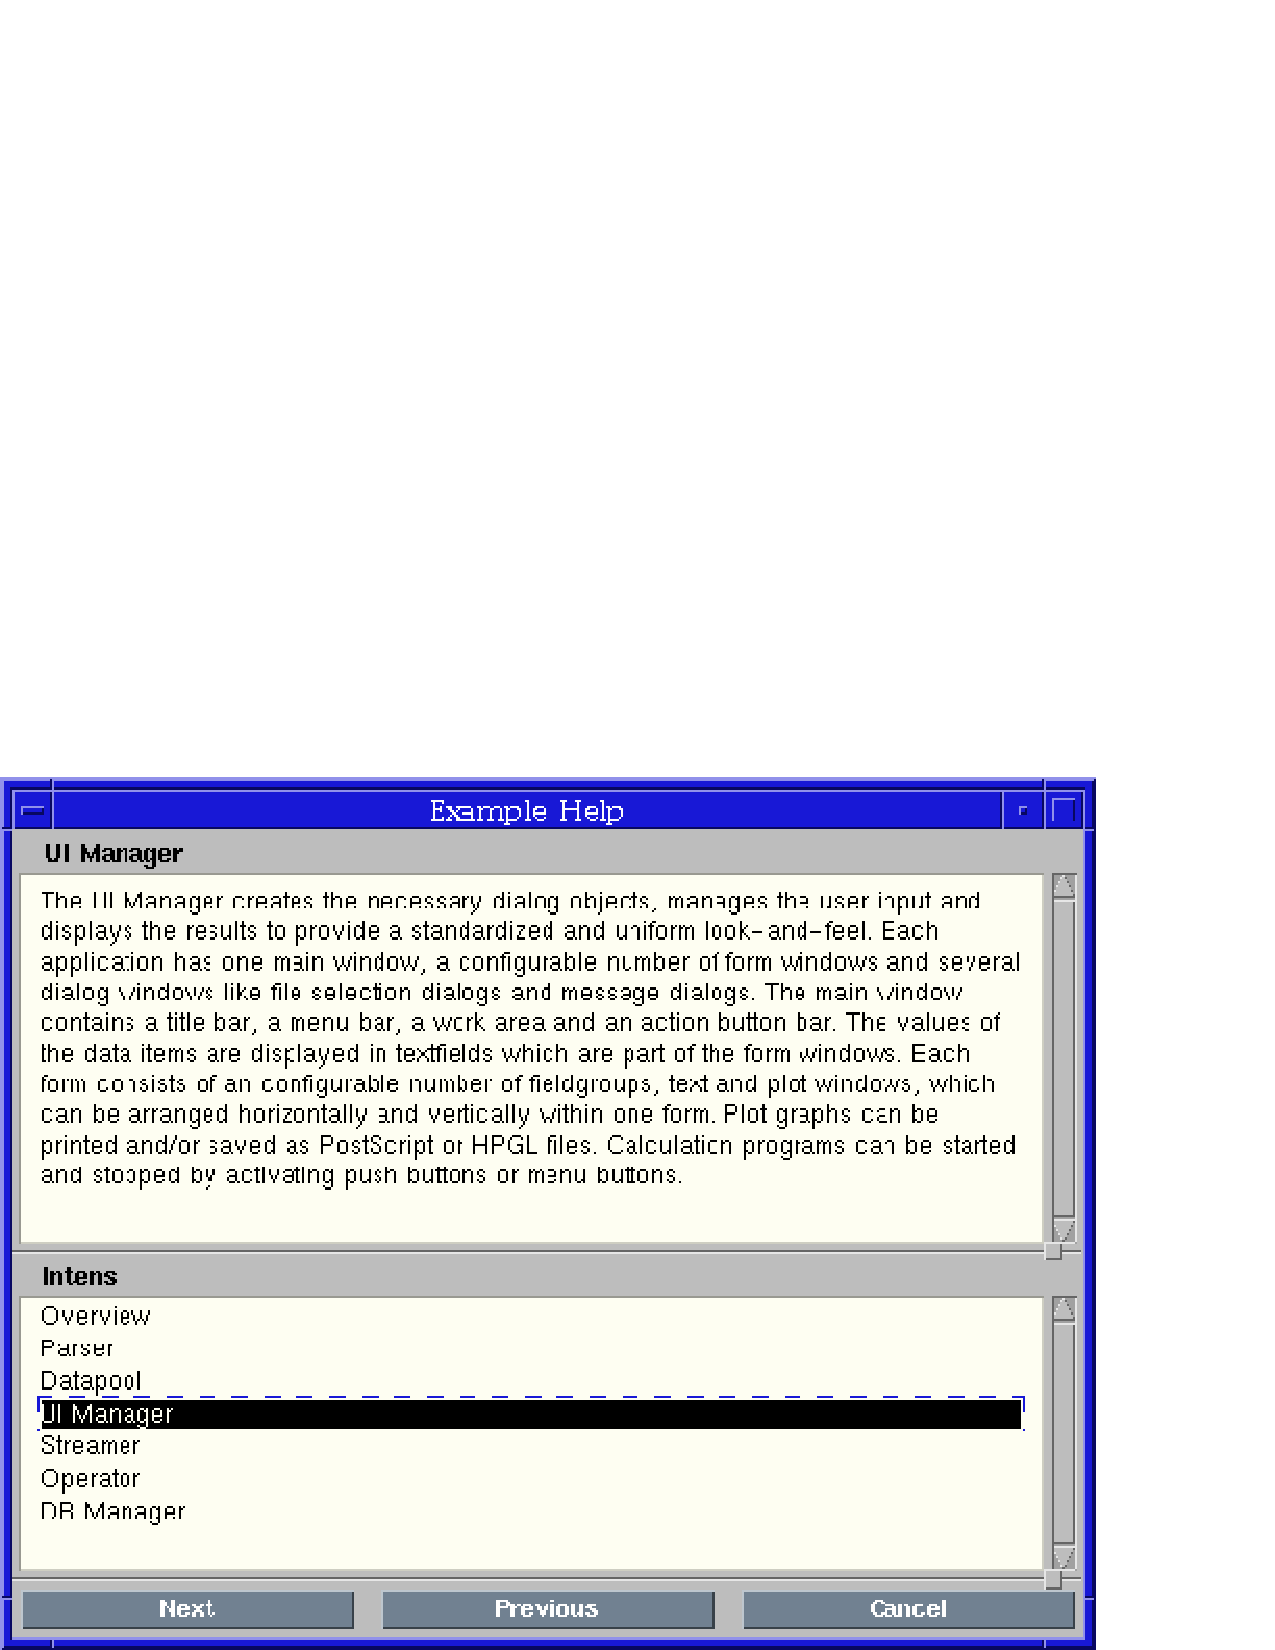
\includegraphics[width=13cm]{grab_helpfile}
   \end{center}
\caption{Example of a Help Window}
\end{figure}

%%%%%%%%%%%%%%%%%%%%%%%%%%%%%%%%%%%%%%%%%%%%%%%%%%%%%%%%%%%%%%%%%%%%%%%%%%%%%
%%%                               HTML                                   %%%
%%%%%%%%%%%%%%%%%%%%%%%%%%%%%%%%%%%%%%%%%%%%%%%%%%%%%%%%%%%%%%%%%%%%%%%%%%%%%
\newpage
\subsubsection{HTML files}
\label{sec:hfbrowser}
For displaying HTML files with the web browser \index{help!Web Browser}
either use \OPENFILE{} or \OPENURL. The specified file
must have a browser readable format such as HTML. \index{help!HTML}
The only thing \INTENS{} does is connecting to the web browser and invoking its open
command (with the \verb+-remote+ command).

\input{diagrams/helpfile_options}
\input{diagrams/helpfile_key}
\index{HELPFILE@\HELPFILE!options}
\index{HIDDEN@\HIDDEN!helpfile option}
\index{HELPKEY@\HELPKEY!helpfile option}

\begin{tabularx}{\textwidth}{l|X}
help\_options        & description \\ \hline
\verb+title_string+  & string: Defines the label in the help menu.
                       The filename is used if there is no title defined.\\
\HIDDEN              & No menu entry will be created for this helpfile.\\
\HELPKEY             & specifies the helpkeys (anchors) that are defined in the HTML file
                       (see chapter \nameref{key:helpkey} on page \pageref{key:helpkey}). \\
\end{tabularx}
\vspace{0.5cm}

If you want to reference specified anchors in your document, then you have
to list them as \HELPKEY s.
The following example shows an anchor named "goHere" in a HTML document:


\begin{boxedminipage}[t]{\linewidth}
\begin{verbatim}
...
<A NAME="goHere"<\A>
...
\end{verbatim}
\end{boxedminipage}


%%%%%%%%%%%%%%%%%%%%%%%%%%%%%%%%%%%%%%%%%%%%%%%%%%%%%%%%%%%%%%%%%%%%%%%%%%%%%
%%%                              Examples                                 %%%
%%%%%%%%%%%%%%%%%%%%%%%%%%%%%%%%%%%%%%%%%%%%%%%%%%%%%%%%%%%%%%%%%%%%%%%%%%%%%
%%\subsubsection{Examples}
\label{sec:helpfileexamples}


\begin{boxedminipage}[t]{\linewidth}
\begin{alltt}
\HELPFILE
  "helpfile.hlp",
  "helpfile\_2.hlp",
  OPEN\_FILE "helpfile.html"  HELPKEY("goHere"),
  OPEN\_URL  "www.semafor.ch"
;
\end{alltt}
\end{boxedminipage}

   \newpage
\subsection{DATAPOOL}
%           --------
\label{sec:datapool}
%%%%%%%%%%%%%%%%%%%%%%%%%%%%%%%%%%%%%%%%%%%%%%%%%%%%%%%%%%%%%%%%%%%%%%%%%%%%%
%%%                             Description                               %%%
%%%%%%%%%%%%%%%%%%%%%%%%%%%%%%%%%%%%%%%%%%%%%%%%%%%%%%%%%%%%%%%%%%%%%%%%%%%%%
\subsubsection{Description}
\label{sec:dpdescription}
\index{DATAPOOL@\DATAPOOL}
All {\bfseries Data Items} used in an \INTENS{}-application are defined in the \DATAPOOL{} section.\\
One of the most important functions of the datapool is the dynamic allocation of memory for these data items.\\
\vspace{0.5cm}
To define {\bfseries STRUCTURES} you have to give an identifier, which will
be used as a data type to define data items later.
(see section \nameref{sec:dpstruct} on page \pageref{sec:dpstruct}).\\
\vspace{0.5cm}
You can define \SET s, which are used by the \UIMANAGER{}
to show values of data items in a Combobox or Option menu.
(see section \nameref{sec:dpset} on page \pageref{sec:dpset}).\\
\vspace{0.5cm}
You can also define \COLOR s, which are used by the \UIMANAGER{}
to show items with different colors corresponding to their values.
(see section \nameref{sec:dpcolorset} on page \pageref{sec:dpcolorset}).\\

\input{diagrams/datapool_description}
\index{DATAPOOL@\DATAPOOL!description}

%%%%%%%%%%%%%%%%%%%%%%%%%%%%%%%%%%%%%%%%%%%%%%%%%%%%%%%%%%%%%%%%%%%%%%%%%%%%%
%%%                              Data Item                                %%%
%%%%%%%%%%%%%%%%%%%%%%%%%%%%%%%%%%%%%%%%%%%%%%%%%%%%%%%%%%%%%%%%%%%%%%%%%%%%%
\newpage
\subsubsection{Data Item}
\label{sec:dpitem}
\index{DATAPOOL@\DATAPOOL!data types}
Since the \DATAPOOL{} allocates memory dynamically, it is
not necessary to declare the dimension of the data items (unsigned integers
between braces).
Nevertheless the declaration is recommended, if
the dimension is known and if it will not change during the calculation
process. Their index range always begins at 0.
See \hyperref[dia:datadimension]{data\_dimension} on page \pageref{dia:datadimension} for the syntax. \\

\input{diagrams/data_item_declaration}
\input{diagrams/data_variable_declaration}
\index{data item!declaration}
\index{INTEGER@\INTEGER!datapool data type}
\index{INT@\INT!datapool data type (see INTEGER)}
\index{REAL@\REAL!datapool data type}
\index{COMPLEX@\COMPLEX!datapool data type}
\index{CDATA@\CDATA!datapool data type}
\index{STRING@\STRING!datapool data type}

\begin{tabularx}{\textwidth}{l|X}
data item           & Description \\
\hline
\verb+identifier+  & data item identifier. It is needed for referencing this data item. \\
\REAL               & defines data items for storing real number values. \\
\INTEGER            & defines data items for storing integer number values. \\
\STRING             & defines data items for storing characters. \\
\COMPLEX            & defines data items for storing {\bfseries complex} quantities. \\
\CDATA              & defines data items for storing character or binary data.
                      (database: mapped to BLOB, no length restrictions while
                       strings are limited to 255 characters) \\
{\bfseries ID\_DATASTRUCTURE} & defines data items for storing structured data. \\
                    & must be a previously defined structure
                      (section \nameref{sec:dpstruct} on page \pageref{sec:dpstruct}) \\
\end{tabularx}
\vspace{0.5cm}

\begin{boxedminipage}[t]{\linewidth}
\begin{intens}
DATAPOOL
  REAL
    data_item_identifier_A[10],        // 1 dimension
    data_item_identifier_B[3,20],      // 2 dimensions
    data_item_identifier_C[2,4,10];    // 3 dimensions

END DATAPOOL;
\end{intens}
\end{boxedminipage}

\vspace{0.5cm}
\input{diagrams/data_dimension}
\index{data dimension!declaration}
\vspace{0.5cm}

Declare the dimension of the data item. See first paragraph in
section \nameref{sec:dpitem} on page \pageref{sec:dpitem} for more information.

\vspace{0.5cm}

\index{DATAPOOL@\DATAPOOL!predefined data items}
The following data items are {\bfseries predefined} by the system at startup
       and must not be redefined: \\
\vspace{0.5cm}
\index{data item!predefined}
\index{DATE@\DATE!predefined datapool item}
\index{USER@\USER!predefined datapool item}
\index{HOST@\HOST!predefined datapool item}
\index{IPADDR@\IPADDR!predefined datapool item}
\index{INTENS\_VERSION@\INTENSVERSION!predefined datapool item}
\index{INTENS\_VERSION\_MAJOR@\INTENSVERSIONMAJOR!predefined datapool item}
\index{INTENS\_VERSION\_MINOR@\INTENSVERSIONMINOR!predefined datapool item}
\index{INTENS\_VERSION\_PATCH@\INTENSVERSIONPATCH!predefined datapool item}
\index{INTENS\_REVISION@\INTENSREVISION!predefined datapool item}
\index{RESTUSERNAME@\RESTUSERNAME!predefined datapool item}
\index{RESTUSERNAMELIST@\RESTUSERNAMELIST!predefined datapool item}
\index{RESTBASE@\RESTBASE!predefined datapool item}
\index{REST\_SERVICE.APP\_VERSION\_MAJOR@\RESTSERVICEAPPVERSIONMAJOR!predefined datapool item}
\index{REST\_SERVICE.APP\_VERSION\_MINOR@\RESTSERVICEAPPVERSIONMINOR!predefined datapool item}
\index{REST\_SERVICE.APP\_VERSION\_PATCH@\RESTSERVICEAPPVERSIONPATCH!predefined datapool item}
\index{REST\_SERVICE.DB\_VERSION\_MAJOR@\RESTSERVICEDBVERSIONMAJOR!predefined datapool item}
\index{REST\_SERVICE.DB\_VERSION\_MINOR@\RESTSERVICEDBVERSIONMINOR!predefined datapool item}
\index{REST\_SERVICE.DB\_VERSION\_PATCH@\RESTSERVICEDBVERSIONPATCH!predefined datapool item}
\index{REST\_SERVICE.DB\_VERSION\_IGNORE@\RESTSERVICEDBVERSIONIGNORE!predefined datapool item}
\index{PLOT2D\_UIMODE@\PLOTTWODUIMODE!predefined datapool item}
\index{PLOT2D\_SYMBOLSIZE@\PLOTTWODSYMBOLSIZE!predefined datapool item}
\index{Global\_Point@\GlobalPoint!predefined datapool item}
\index{Global\_Rect@\GlobalRect!predefined datapool item}
\label{dataitempredefined}
\begin{tabularx}{\textwidth}{l|X}
Itemname    & Description \\
\hline
\DATE       & contains the current date (yyyy-mm-dd, \STRING) \\
\USER       & contains the user name (\STRING) \\
\HOST       & hostname of the working machine (use VAR(``HOST'') to access it, \STRING) \\
\IPADDR     & ip address of the working machine (\STRING) \\
\INTENSVERSION & \INTENS{} version (i.E. 5.3.1/5.3.2dev, \STRING) \\
\INTENSVERSIONMAJOR & \INTENS{} MAJOR version (i.E. 5, \INTEGER) \\
\INTENSVERSIONMINOR & \INTENS{} MINOR version (i.E. 3, \INTEGER) \\
\INTENSVERSIONPATCH & \INTENS{} PATCH version (i.E. 1/2dev, \STRING) \\
\INTENSREVISION & \INTENS{} revision (i.E. -/67-g0df41633, \STRING) \\
\RESTUSERNAME  & username used to login to the RESTful web service (\STRING) \\
\RESTUSERNAMELIST  & list of usernames to show in login dialog for RESTful web service (\STRING) \\
\RESTBASE   & base url of the RESTful web service (\STRING) \\
\RESTSERVICEAPPVERSIONMAJOR & see paragraph \nameref{par:restServiceVersionControl}
              on page \pageref{par:restServiceVersionControl} (\INTEGER) \\
\RESTSERVICEAPPVERSIONMINOR & see paragraph \nameref{par:restServiceVersionControl}
              on page \pageref{par:restServiceVersionControl} (\INTEGER) \\
\RESTSERVICEAPPVERSIONPATCH & see paragraph \nameref{par:restServiceVersionControl}
              on page \pageref{par:restServiceVersionControl} (\INTEGER) \\
\RESTSERVICEDBVERSIONMAJOR & see paragraph \nameref{par:restServiceVersionControl}
              on page \pageref{par:restServiceVersionControl} (\INTEGER) \\
\RESTSERVICEDBVERSIONMINOR & see paragraph \nameref{par:restServiceVersionControl}
              on page \pageref{par:restServiceVersionControl} (\INTEGER) \\
\RESTSERVICEDBVERSIONPATCH & see paragraph \nameref{par:restServiceVersionControl}
              on page \pageref{par:restServiceVersionControl} (\INTEGER) \\
\RESTSERVICEDBVERSIONIGNORE & see paragraph \nameref{par:restServiceVersionControl}
              on page \pageref{par:restServiceVersionControl} (\INTEGER) \\
\PLOTTWODUIMODE  & see paragraph \nameref{par:uiplot2duimode} in section \nameref{sec:uiplot2d}
              on page \pageref{par:uiplot2duimode} (\STRING) \\
\PLOTTWODSYMBOLSIZE  & see paragraph \nameref{par:uiplot2symbolsize} in section \nameref{sec:uiplot2d}
              on page \pageref{par:uiplot2symbolsize} (\INTEGER) \\
\GlobalPoint & structure object with data items X, Y and Y2 \newline
              Used in UI Mode ``Select Point''.
              See paragraph \nameref{par:uiplot2duimode} in section \nameref{sec:uiplot2d}
              on page \pageref{par:uiplot2duimode} \\
\GlobalRect & structure object with data items X1, Y1, X2 and Y2 \newline
              Used in UI Mode ``Select Rectangle''.
              See paragraph \nameref{par:uiplot2duimode} in section \nameref{sec:uiplot2d}
              on page \pageref{par:uiplot2duimode} \\
%% \ProgressDialog & structure object with data items MainTitle, MainPercent, SubTitle, SubPercent, ErrorString \newline
%%               TODO \\
%% \ProgressDialogAbortCommand & TODO (\STRING) \\
%% \ProgressDialogLoopTitle & TODO (\STRING) \\
\end{tabularx}

\input{diagrams/data_variable_attributes}
\index{DATAPOOL@\DATAPOOL!data item attributes}

\index{EDITABLE@\EDITABLE!datapool attributes}
\index{OPTIONAL@\OPTIONAL!datapool attributes}
\index{LOCKABLE@\LOCKABLE!datapool attributes}
\index{SCALAR@\SCALAR!datapool attributes}
\index{CELL@\CELL!datapool attribute}
\index{GLOBAL@\GLOBAL!datapool attribute}
\index{OMIT\_TTRAIL@\OMITTTRAIL!datapool attribute}
\index{NO\_DEPENDENCIES@\NODEPENDENCIES!datapool attribute}
\index{CLASSNAME@\CLASSNAME!datapool attributes}
\label{dataitemattributes}
\begin{tabularx}{\textwidth}{l|X}
Attributes       & Description \\ \hline
\EDITABLE        & The value can be changed (edited) by the user
                   (see also section
                   \nameref{sec:uimanager} on page \pageref{sec:uimanager})\\
\OPTIONAL        & Same as \EDITABLE. The corresponding text fields
                   may be given different %%X resources
                   foreground/background color, font etc. \\
                   %%(see section \nameref{sec:x-resources} on page
                   %%\pageref{sec:x-resources})\\
\LOCKABLE        & The data item can be protected against being overwritten
                   by stream operations.
                   (see also section
                   \nameref{sec:uimanager} on page \pageref{sec:uimanager})\\
\SCALAR          & Data items with this attribute are transferred as scalars
                   instead of matrices to any Matlab function
                   (or instread of vectors to and from the database).
                   They are not written as a list in a \JSON{} \STREAM.\\
\CELL            & The data item is transferred to the Matlab workspace as cell instead of array. \\
\GLOBAL          & The data item is not changed by cycle operations. \\
\OMITTTRAIL      & The data item is not handled by transactions (ABORT, UNDO, ...). \\
\NODEPENDENCIES  & No dependencies between this input and its outputs (results) are added.
                   (see paragraph \nameref{par:stdependency} on page \pageref{par:stdependency}) \\
\CLASSNAME       & Data items having a classname are transferred as
                   objects to any Matlab function. \newline
                   The \CLASSNAME{} can also be used in \FUNCTIONS: \CLASSNAME(item). \\
\end{tabularx}

\index{data item!options}
\input{diagrams/data_item_options}
\index{DATAPOOL@\DATAPOOL!data item options}
\index{SET@\SET!datapool item option}
\index{INDEXED\_SET@\INDEXEDSET!datapool item option}
\index{COLOR@\COLOR!datapool item option}
\index{NO\_COLORBIT@\NOCOLORBIT!datapool item option}
\index{FUNC@\FUNC!datapool item option}
\index{LABEL@\LABEL!datapool item option}
\index{UNIT@\UNIT!datapool item option}
\index{UNITS (see UNIT)}
\index{PATTERN@\PATTERN!datapool item option}
\index{HELPTEXT@\HELPTEXT!datapool item option}
\index{BUTTON@\BUTTON!datapool item option}
\index{SLIDER@\SLIDER!datapool item option}
\index{PROGRESS@\PROGRESS!datapool item option}
\index{RANGE@\RANGE!datapool item option}
\index{STEP@\STEP!datapool item option}
\index{TOGGLE@\TOGGLE!datapool item option}
\index{RADIO@\RADIO!datapool item option}
\index{CLASSNAME@\CLASSNAME!datapool item option}
\index{SCALAR@\SCALAR!datapool item option}
\index{CELL@\CELL!datapool item option}
\index{HIDDEN@\HIDDEN!datapool item option}
\index{PLACEHOLDER@\PLACEHOLDER!datapool item option}

\input{diagrams/data_item_more_option}
\index{PERSISTENT@\PERSISTENT!datapool item option}
\index{TRANSIENT@\TRANSIENT!datapool item option}
\index{DBATTR@\DBATTR!datapool item option}
\index{DBUNIT@\DBUNIT!datapool item option}
\index{TAG@\TAG!datapool item option}
\index{FOLDER@\FOLDER!datapool item option}
\index{NONE@\NONE!datapool item option}
\index{STRING\_DATE@\STRINGDATE!datapool item option}
\index{STRING\_TIME@\STRINGTIME!datapool item option}
\index{STRING\_DATETIME@\STRINGDATETIME!datapool item option}
\index{PASSWORD@\PASSWORD!datapool item option}
\index{WHEEL\_EVENT@\WHEELEVENT!datapool item option}

\begin{tabularx}{\textwidth}{l|X}
Options          & Description \\ \hline
\SET             & The items values are part of a \SET. A set is a limited number of values of the same type.
                   The item is displayed as Combobox on the user interface.
                   \verb+ID_DATASET+ must be previously defined (see section \nameref{sec:dpset} page \pageref{sec:dpset})\\
\INDEXEDSET      & Like \SET. When the data item is used as a vector, each element can have a different
                   list of values to select from. \\
\COLOR{} = ...   & The field is shown in the colors that corresponds to its items value.
                   \verb+ID_COLORSET+ must be previously defined (see section \nameref{sec:dpcolorset} page \pageref{sec:dpcolorset})\\
\COLOR           & String data item to define a color.
                   The item is displayed as a color picker: a button that shows the color.
                   Pressing the button opens a color dialog to choose a color.
                   The chosen color is stored as the value of the variable. \\
\NOCOLORBIT      & The eight available color bits (see section \nameref{fu:set:statement} page \pageref{fu:set:statement}) are interpreted as a
                   8-bit number. This gives the possibility to use up to 255 different colors. \\
\FUNC            & Defines the function that will be called after an interactive modification
                   of the items value.
                   (see also section \nameref{sec:functions} on page \pageref{sec:functions})\\
\LABEL{} = ...   & The item has a label which can be used by the \UIMANAGER{} and \STREAMER.
                   (see also section \nameref{sec:uifieldgroup} on page \pageref{sec:uifieldgroup}) \\
\UNIT            & The item has a unit which can be used by the \UIMANAGER{} and \STREAMER.
                   (see also section \nameref{sec:uifieldgroup} on page \pageref{sec:uifieldgroup})\\
\PATTERN         & A regular expression that defines the possible input values. \\
\HELPTEXT        & For each item a helptext may be defined.
                    This text appears as soon as the mouse-pointer crosses the field,
                   which contains the data-item.\\
\BUTTON          & The item is displayed as button on the user interface.
                    Activating the button executes the associated function
                   (see above \FUNC).\\
\SLIDER          & The item is displayed as a slider. \\
\PROGRESS        & The item is displayed as a progress bar. \newline
                   This makes it possible to show a progress bar inside a \FIELDGROUP{}. Assign the desired
                   value (from 0 to 100) to the (integer) variable and the item shows the progress. \\
\RANGE           & Minimal and maximal values for a \SLIDER. \\
\STEP            & Difference between the labels of \SLIDER. \\
\TOGGLE          & The item is displayed as Toggle on the user interface.
                   Activating the toggle changes the value from 0 to 1,
                   deactivating changes the value from 1 to 0.
                   A variable that has no value (invalid) is shown as a deactivated toggle,
                   just as a variable with the value 0. \\
\RADIO           & The item is displayed as ragio button on the user interface.
                   Activating the radio button changes the value from 0 to 1,
                   deactivating changes the value from 1 to 0.
                   A variable that has no value (invalid) is shown as a deactivated radio button,
                   just as a variable with the value 0. \\
\LABEL           & The item is displayed as a label (not editable).\\
\CLASSNAME       & Data items having a classname are transferred as objects to the Matlab workspace. \newline
                   The \CLASSNAME{} can also be used in \FUNCTIONS: \CLASSNAME(item) \\
\SCALAR          & Data items with this attribute are transferred as scalars
                      instead of matrices to the Matlab workspace
                      (or instread of vectors to and from the database).
                      They are not written as a list in a \JSON{} \STREAM.\\
\CELL            & The data item is transferred to Matlab workspace as cell instead of array. \\
\HIDDEN          & The data item is not transferred to Matlab.
                   It is, by default, not written in \JSON{} \STREAM{}s (see \nameref{dia:stjsonoptions} on page \pageref{dia:stjsonoptions}).
                   It is however sent to the rest service (see \nameref{dia:restServicestatement} on page \pageref{dia:restServicestatement}).\\
\PLACEHOLDER     & For each item a placeholder text may be defined.
                   This text appears in the field which contains the data-item when it is \INVALID.\\
\PERSISTENT      & This data item can be stored to and retrieved from the database.\\
\TRANSIENT       & This data item is not stored to and retrieved from the database.
                   It is useful in a \PERSISTENT{} \STRUCT.\\
\DBATTR          & defines the corresponding db attribute name.\\
\DBUNIT          & defines the corresponding db attribute unit.\\
\TAG             & The TAG-identifier is referenced by the navigators COL-definition.
                   (see section \nameref{sec:uinavigatoroptions} on page \pageref{sec:uinavigatoroptions})\\
%%\FOLDER{} = \NONE  & verhindert, dass die Struktur im Navigator als Folder dargestellt wird.\\
\STRINGDATE      & String data item to show and enter a date (popup calendar may be used).\\
\STRINGTIME      & String data item to show and enter a time.\\
\STRINGDATETIME  & String data item to show and enter a date and time.\\
\PASSWORD        & String data item is displayed in password mode.\\
\WHEELEVENT      & The mouse wheel can be used to increment and decrement the value,
                   just as the up and down keys can be used for every numeric data item. \newline
                   This does not work when commandline option \texttt{--}withoutArrowKeys is given. \newline
                   This option enables the mouse wheel event for one numeric data item,
                   whereas the commandline option \texttt{--}withWheelEvent enables it for every numeric data item. \\
\end{tabularx}

\begin{multicols}{2}
\input{diagrams/data_tags}
\input{diagrams/data_tag}
\end{multicols}

\begin{tabularx}{\textwidth}{l|X}
tag          & Description \\ \hline
{\bfseries IDENTIFIER} & Defines a new tag. \\
{\bfseries ID\_TAG} & References an existing tag. \\
\end{tabularx}

%%%%%%%%%%%%%%%%%%%%%%%%%%%%%%%%%%%%%%%%%%%%%%%%%%%%%%%%%%%%%%%%%%%%%%%%%%%%%
%%%                              Data Set                                 %%%
%%%%%%%%%%%%%%%%%%%%%%%%%%%%%%%%%%%%%%%%%%%%%%%%%%%%%%%%%%%%%%%%%%%%%%%%%%%%%
\newpage
\subsubsection{Data Set}
\label{sec:dpset}
\index{DATAPOOL@\DATAPOOL!data set}
Data sets are used for assigning labels to data items. Data sets may be assigned
to data items using the option SET=data-set\_identifier of a previously declared
data set. (section \nameref{dia:dataitemoptions} on page \pageref{dia:dataitemoptions}) \\
By editing such a data item the associated label-strings are shown, while the corresponding
values are transferred to the external process.\\

\input{diagrams/set_declaration}
\input{diagrams/data_set_attr}
\input{diagrams/data_set_item}
\index{SET@\SET}
\index{SET@\SET!datapool data set}

\index{GLOBAL@\GLOBAL!data set option}
\index{INVALID@\INVALID!data set option INVALID=NONE}
\index{NONE@\NONE!data set option INVALID=NONE}
\begin{tabularx}{\textwidth}{l|X}
Option           & Description \\ \hline
\GLOBAL          & The data set is not changed by cycle operations. \\
\INVALID=\NONE   & No empty (invalid) entry is created. \\
\end{tabularx}
\vspace{0.5cm}

The label-strings of a set define the option menu labels. The value types
can be \REAL, \INTEGER{} or \STRING.
The values correspond to the text of the label.
If the values are missing, \INTENS{} assumes increasing integer numbers
starting at 0 for real and integer items. String items contain the string itself.


\begin{boxedminipage}[t]{\linewidth}
\begin{intens}
DATAPOOL
  SET
    set_identifier ( "circle" = 0, "triangle" = 1, "square"= 2 );

  INTEGER {EDITABLE}
    data_item_identifier {SET = set_identifier};

END DATAPOOL;
\end{intens}
\end{boxedminipage}

%%%%%%%%%%%%%%%%%%%%%%%%%%%%%%%%%%%%%%%%%%%%%%%%%%%%%%%%%%%%%%%%%%%%%%%%%%%%%
%%%                              Dynamic Combobox                         %%%
%%%%%%%%%%%%%%%%%%%%%%%%%%%%%%%%%%%%%%%%%%%%%%%%%%%%%%%%%%%%%%%%%%%%%%%%%%%%%
\newpage
\subsubsection{Dynamic Combobox}
\index{STRING@\STRING!dynamic combobox}
\label{stringdynamiccombobox}
Sometimes it is not possible to use a \SET{} to build a combobox. Then, a \STRING{}
item can be changed to a combobox by assigning a special value to it:

\verb+{"value": "a", "input":["A","B","C",null], "output":["a","b","c",null]}+

It must be a JSON object with the members:
\begin{itemize}
  \item \Slanted{value}: the selected value. One of the values of \Slanted{output}.
  \item \Slanted{input}: list of strings. The elements presented to the user in a combobox.
  \item \Slanted{output}: list of values (normally strings). The values corresponding to the \Slanted{input} values.
\end{itemize}
When the first element of \Slanted{input} is selected, \Slanted{value} is set to the first element of \Slanted{output}. \\
To extract the \Slanted{value} from the total string in a function, use \STRINGVALUE{}(item).


%%%%%%%%%%%%%%%%%%%%%%%%%%%%%%%%%%%%%%%%%%%%%%%%%%%%%%%%%%%%%%%%%%%%%%%%%%%%%
%%%                             Data ColorSet                             %%%
%%%%%%%%%%%%%%%%%%%%%%%%%%%%%%%%%%%%%%%%%%%%%%%%%%%%%%%%%%%%%%%%%%%%%%%%%%%%%
\newpage
\subsubsection{Data ColorSet}
\label{sec:dpcolorset}
\index{DATAPOOL@\DATAPOOL!data colorset}
Data colorsets are used for assigning colors to values. Data colorsets may be assigned
to data items using the option COLOR=data-colorset\_identifier of a previously declared
data colorset. (section \nameref{dia:dataitemoptions} on page \pageref{dia:dataitemoptions}) \\
The field of such a data item will change to the associated colors that correspond to its value.\\

\input{diagrams/color_declaration}
\input{diagrams/data_colorset_item}
\index{COLOR@\COLOR}
\index{COLOR@\COLOR!datapool data set}

\begin{tabularx}{\textwidth}{l|X}
value                       & Description \\
\hline
\INVALID                    & invalid value. \\
\verb+data colorset value+  & less than, more than or exaclty one specific value
                              (see paragraph \nameref{par:dpcolorsetvaluerange} on page \pageref{par:dpcolorsetvaluerange}).\\
\verb+data colorset range+  & data range (see paragraph \nameref{par:dpcolorsetvaluerange} on page \pageref{par:dpcolorsetvaluerange}).\\
\ELSE                       & all other values (not matched by any other colorset item values). \\
\end{tabularx}
\vspace{0.5cm}

The pair of bg\_color\_string and fg\_color\_string of a colorset define the
background and foreground color used for value defined on the left. \\
The color-string may be in one of these formats:
\begin{itemize}
  \item \#RGB (each of R, G and B is a single hex digit)
  \item \#RRGGBB
  \item A name from the list of colors defined in the list of
  \href{http://www.w3.org/TR/SVG/types.html#ColorKeywords}{SVG color keyword names}
  provided by the World Wide Web Consortium;
  for example, "steelblue" or "gainsboro". These color names work on
  all platforms.
\end{itemize}

Instead of providing static color-strings, the colors can also be a data reference. If the data item has
a valid color string value, that value is used. This can be used i.E. to change the color of plot curves
(see section \nameref{sec:uiplot2d} on page \pageref{sec:uiplot2d}).

\newpage
\paragraph{Data ColorSet Value and Range}
\label{par:dpcolorsetvaluerange}
~\\[0.5cm]

\input{diagrams/data_colorset_value}
\input{diagrams/data_colorset_range}

\begin{tabularx}{\textwidth}{l|X}
value                    & Description \\
\hline
\verb+real or int value+ & any value or mathematical 'combination' as shown in the example
                           in section \nameref{sec:scale} on page \pageref{sec:scale}. \\
\verb+string+            & any string constant or 'combination'.
                           (see section \nameref{sec:string} on page
                           \pageref{sec:string}) \\
\verb+range data reference+ & references a data item declared in the datapool
                             (section \nameref{sec:rangedatareference} on page
                              \pageref{sec:rangedatareference}). \\
\end{tabularx}
\vspace{0.5cm}

\begin{boxedminipage}[t]{\linewidth}
\begin{intens}
DATAPOOL
  COLOR
    red_green_blue_color (
      INVALID = ( "red", "black" ),
      < 0     = ( "#fff", "#f00" ),
      RANGE ( 0, <2 ) = ( "#ffffff", "#00ff00" ),
      2 = ( "#ffffff", "#0000ff" ),
      ELSE = ( "#ffffff", "#0000ff" )
    )
  ;

  INTEGER {EDITABLE}
    data_item_identifier {COLOR = red_green_blue_color};

END DATAPOOL;
\end{intens}
\end{boxedminipage}

%%%%%%%%%%%%%%%%%%%%%%%%%%%%%%%%%%%%%%%%%%%%%%%%%%%%%%%%%%%%%%%%%%%%%%%%%%%%%
%%%                     Structured Data Items                             %%%
%%%%%%%%%%%%%%%%%%%%%%%%%%%%%%%%%%%%%%%%%%%%%%%%%%%%%%%%%%%%%%%%%%%%%%%%%%%%%
\newpage
\subsubsection{Structure definition}
\label{sec:dpstruct}
\index{DATAPOOL@\DATAPOOL!data structure}
\index{DATAPOOL@\DATAPOOL!struct}
Data items may be grouped in structures. This enhances the possibilities
of storing and transmitting data. \\
A structure holds several data items of any valid data type described in
section \nameref{sec:dpitem} on page \pageref{sec:dpitem}.

\input{diagrams/structure_declaration}
\index{STRUCT@\STRUCT}
\index{STRUCT@\STRUCT!inheritance}
\index{  @Signs / Characters!: (colon)!structure inheritance}

\begin{tabularx}{\textwidth}{l|X}
Structure definition            & Description \\
\hline
{\bfseries ID\_DATASTRUCTURE}   & identifier of previously defined structure. \\
                                & inherit definition of this struct. \\
\verb+data item declaration+ & see section \nameref{sec:dpitem} on page \pageref{sec:dpitem}. \\
\end{tabularx}
\vspace{0.5cm}



\begin{boxedminipage}[t]{\linewidth}
\begin{intens}
DATAPOOL
  STRUCT structure_def
  {
     INTEGER {EDITABLE}
        data_item_identifier_1,
        data_item_identifier_2;
     REAL {OPTIONAL}
        data_item_identifier_3;
  };

  structure_def
    structure_identifier_1,
    structure_identifier_2;

END DATAPOOL;
\end{intens}
\end{boxedminipage}


%%%%%%%%%%%%%%%%%%%%%%%%%%%%%%%%%%%%%%%%%%%%%%%%%%%%%%%%%%%%%%%%%%%%%%%%%%%%%
%%%                              Examples                                 %%%
%%%%%%%%%%%%%%%%%%%%%%%%%%%%%%%%%%%%%%%%%%%%%%%%%%%%%%%%%%%%%%%%%%%%%%%%%%%%%
\newpage
\subsubsection{Examples}
\label{sec:dpexamples}


\begin{boxedminipage}[t]{\linewidth}
\begin{intens}
DESCRIPTION "Example of data defining and referring"

DATAPOOL
  SET shape_set ( "circle" = 0, "triangle" = 1, "square"= 2 );

  STRUCT Object {
     INTEGER {EDITABLE}
        shape {SET = shape_set,COMBOBOX
              ,LABEL = "The Shape"};
     REAL {OPTIONAL}
        size  {LABEL = "The Size", UNIT = "cm"};
  };

  Object obj[20];

  STRING {EDITABLE, SCALAR}
     text;

END DATAPOOL;

UIMANAGER
  FIELDGROUP
    fieldgroup_identifier
    (
      "Select first shape:" obj[0].shape,
      "Enter first size:"   obj[0].size,

      "Select last shape:"  obj[19].shape,
      "Enter last size:"    obj[19].size,

      "Enter a remark:"     text
    )
  ;

  FORM
    form_identifier {MAIN}
    (
      (fieldgroup_identifier)
    )
  ;

END UIMANAGER;

\end{intens}
\end{boxedminipage}

   \newpage
\subsubsection{Data Reference}
%              --------------
\label{sec:tempdatareference}
%%%%%%%%%%%%%%%%%%%%%%%%%%%%%%%%%%%%%%%%%%%%%%%%%%%%%%%%%%%%%%%%%%%%%%%%%%%%%
%%%                          Temp Data Reference                          %%%
%%%%%%%%%%%%%%%%%%%%%%%%%%%%%%%%%%%%%%%%%%%%%%%%%%%%%%%%%%%%%%%%%%%%%%%%%%%%%
Temp Data Reference references a data item declared in the datapool 
(section \nameref{sec:dpitem} page \pageref{sec:dpitem}): \\

\input{diagrams/temp_data_reference}

\index{Temp Data Reference}
\index{  @Signs / Characters!. (dot)!structure item separator}
\begin{tabularx}{\textwidth}{l|X}
option            & Description \\
\hline
\verb+ui field indizes+ & optional indizes (see page \pageref{uifieldindizes}). \\
\verb+.+          & structure item separator \\
                  & Structures are explained in section \nameref{sec:dpstruct}
                  page \pageref{sec:dpstruct}\\
\verb+identifier+ & references a data item declared in datapool (section 
              \nameref{sec:dpitem} page \pageref{sec:dpitem}). For options like
              \LABEL{} and \UNIT{} use data items without indexes. \\
\end{tabularx}

\vspace{3cm}

\label{sec:rangedatareference}
%%%%%%%%%%%%%%%%%%%%%%%%%%%%%%%%%%%%%%%%%%%%%%%%%%%%%%%%%%%%%%%%%%%%%%%%%%%%%
%%%                          Range Data Reference                          %%%
%%%%%%%%%%%%%%%%%%%%%%%%%%%%%%%%%%%%%%%%%%%%%%%%%%%%%%%%%%%%%%%%%%%%%%%%%%%%%
Range Data Reference references a data item declared in the datapool
(section \nameref{sec:dpitem} page \pageref{sec:dpitem}): \\

\input{diagrams/range_data_reference}

\index{Range Data Reference}
\index{Scale factors!Range Data Reference}
\begin{tabularx}{\textwidth}{l|X}
option            & Description \\
\hline
\verb+scale factor+      & a scale factor (see section \nameref{sec:scale} page \pageref{sec:scale}). \\
\verb+st data reference+ & references a data item declared in datapool
                    (section \nameref{sec:stvariables} on page
                     \pageref{fig:st_data_reference}). \\
\end{tabularx}

   \newpage
\subsection{STREAMER}
%           ---------
\label{sec:streamer}
%%%%%%%%%%%%%%%%%%%%%%%%%%%%%%%%%%%%%%%%%%%%%%%%%%%%%%%%%%%%%%%%%%%%%%%%%%%%%
%%%                             Description                               %%%
%%%%%%%%%%%%%%%%%%%%%%%%%%%%%%%%%%%%%%%%%%%%%%%%%%%%%%%%%%%%%%%%%%%%%%%%%%%%%
\subsubsection{Description}
\label{sec:stdescription}
The Streamer manages all input and output formats. A stream consists
of a sequence of data items and string constants.

\paragraph{Dependency}
\label{par:stdependency}
Together with the
datapool and the operator, the streamer controls the dependencies
between input and output variables (datapool items).
In order to keep the data consistent,
all data items that belong to an output stream are set invalid
when one of the items of a corresponding input stream is modified.

Dependencies between input and output \STREAM{}s are defined through
\PROCESSGROUP{}s and \MESSAGEQUEUE{} \REQUEST{}s. They are activated
when the \PROCESSGROUP{} or the \MESSAGEQUEUE{} \REQUEST{} is run.

The user is asked for confirmation before dependencies are cleared
- unless the option \AUTOCLEARDEPENDENCIES{} is used.

\STREAM{}s can be excluded from dependencies using the option \NODEPENDENCIES{}
(see \nameref{dia:jobmessagequeueoption} on page \pageref{dia:jobmessagequeueoption} or
\nameref{dia:jobpluginoption} on page \pageref{dia:jobpluginoption}) or by not giving
a dependency option and using the \INTENS command line argument
\texttt{--}defaultMessageQueueDependencies false.

\input{diagrams/streamer_description}
\index{STREAMER@\STREAMER}

%%%%%%%%%%%%%%%%%%%%%%%%%%%%%%%%%%%%%%%%%%%%%%%%%%%%%%%%%%%%%%%%%%%%%%%%%%%%%
%%%                              IO Stream                                %%%
%%%%%%%%%%%%%%%%%%%%%%%%%%%%%%%%%%%%%%%%%%%%%%%%%%%%%%%%%%%%%%%%%%%%%%%%%%%%%
\subsubsection{IO Stream}
\label{sec:ststream}
\input{diagrams/st_declaration}
\vspace{1cm}

\index{XML@\XML!streamer format command}
\index{JSON@\JSON!streamer format command}

A stream is used to read or write to or from data items, referencing them by their identifier. \\
\vspace{1cm}

A stream is a sequence of format commands that has a unique identifier.
An identifier within a format command references a data item.
If an identifier is preceeded by an exclamation mark it will be checked
to have a valid value before the corresponding calculation program
is called. Item values that are not valid will not be transferred.

The streamer adds one blank character (see \DELIMITER{} on page \pageref{dia:stoptionlist}) after data items to separate them.
This blank character is added only after data items and indices without
a fixed width
 (see {\bfseries field conversion} on page \pageref{par:fieldconversion}
  and {\bfseries field length} on page \pageref{par:stfieldlength}).
\index{  @Signs / Characters!: (colon)!streamer dataitem-format width}
\index{width}

The line containing the \XML{} token defines an xml stream
(see section \nameref{sec:stxmlcommand} on page \pageref{sec:stxmlcommand}).

The line containing the \JSON{} token defines an json stream
(see section \nameref{sec:stjsoncommand} on page \pageref{sec:stjsoncommand}).

Stream identifiers are registered datapool items and contain the filename
(if any) of their last read or write operation.

\input{diagrams/st_option_list}
\index{LATEX@\LATEX!stream option}
\index{URL@\URL!stream option}
\index{DELIMITER@\DELIMITER!stream delimiter}
\index{LOCALE@\LOCALE!stream option}
\index{PROCESS@\PROCESS!stream filter process}
\index{APPEND@\APPEND!stream option}
\index{NO\_GZ@\NOGZ!stream option}
\index{FILE@\FILE!stream option}

\begin{tabularx}{\textwidth}{l|X}
option                   & Description \\
\hline
\LATEX                   & \LaTeX{} special characters
                           (i.E. \textbackslash{} \textasciicircum{} \textbar{} or \{)
                           are replaced with their \LaTeX{} command. \\
\URL                     & reserved characters are percent-encoded and no \DELIMITER{}s are added. \\
\DELIMITER               & defines the character used to separete stream items.
                           default is the blank character. \\
\LOCALE                  & stream uses locale decimal separator. \\
\PROCESS                 & defines a filter process.
                           The streams data is processed by the filter process. \\
\APPEND                  & append received data to the \CDATA{} element of the \STREAM. \\
\NOGZ                    & Stream content is not gunzipped when reading a file stream,
                           although the filename ends in '.gz'. \\
\FILE                    & write to or read from a temporary file instead of the \DATAPOOL. \newline
                           This reduces memory needed by \INTENS{}, but values are not in the \DATAPOOL. \\
\end{tabularx}
\vspace{0.5cm}

Not all combinations are allowed:
\begin{itemize}

\item \LATEX{} or \URL{} \\
      you can only choose one filter

\item \URL{} : no \DELIMITER{} \\
      No \DELIMITER{}s are added with \URL{} option

\end{itemize}

\input{diagrams/st_format_command}
\label{fig:st_format_command}
\index{  @Signs / Characters!\texttt{"!} (exclamation mark)!streamer validation check}
\index{  @Signs / Characters!\# (hash)!streamer index repesent.}
\index{  @Signs / Characters!: (colon)!streamer skip width}
\index{MATRIX@\MATRIX!streamer format command}
\index{Scale factors!streamer}
\index{DATASET\_TEXT@\DATASETTEXT!streamer format command}
\index{SET@\SET!dataset\_text streamer format command}
\index{STRING\_DATE@\STRINGDATE!streamer format command}
\index{STRING\_TIME@\STRINGTIME!streamer format command}
\index{STRING\_DATETIME@\STRINGDATETIME!streamer format command}
\index{STRING\_VALUE@\STRINGVALUE!streamer format command}
\index{PLOTGROUP@\PLOTGROUP!streamer format command}
%%\index{XMLGROUP@\XMLGROUP!streamer format command}
\index{SKIP@\SKIP!streamer format command}
\index{EOLN@\EOLN!streamer format command}

\input{diagrams/st_plotgroup_option}
\label{fig:st_plotgroup_option}
\index{RANGE@\RANGE!streamer plotgroup option}
\index{TRANSPARENT@\TRANSPARENT!streamer plotgroup option}

\begin{tabularx}{\textwidth}{l|X}
format command        & description \\
\hline
{\bfseries !}         & perform a validation check \\
\verb+data reference+ & the possibly indexed data item
                        (see section \nameref{sec:stvariables} page \pageref{fig:st_data_reference}) \\
\MATRIX               & The data item will be transferred as a matrix (see section
                         \nameref{sec:stmatrix} page \pageref{sec:stmatrix}) \\
\verb+scale factor+   & see section \nameref{sec:scale} page
                      \pageref{sec:scale}. \\
                      & The value of the data item is multiplied by the scale factor on
an output operation and divided by the scale factor on an input operation. \\
\verb+field conversion+ & see page \pageref{par:fieldconversion}. \\
\DATASETTEXT          & includes the string of the \SET{} associated with the item (can only be
                        used if the item has a \SET) \\
\STRINGDATE           & prints the date in the local format (i.E. 24.01.08 instead of 2008-01-24)
                    ( see section \nameref{dia:dataitemoptions} on page \pageref{dia:dataitemoptions} ) \\
\STRINGTIME           & prints the time in the local format (i.E. 15:08:00:000 instead of 15:08:00)
                    ( see section \nameref{dia:dataitemoptions} on page \pageref{dia:dataitemoptions} ) \\
\STRINGDATETIME       & prints the date-time in the local format (i.E. 24.01.08 15:08 instead of 2008-01-24T15:08:00)
                    ( see section \nameref{dia:dataitemoptions} on page \pageref{dia:dataitemoptions} ) \\
\STRINGVALUE          & extracts the value of a dynamic \COMBOBOX{}
                    ( see section \nameref{stringdynamiccombobox} on page \pageref{stringdynamiccombobox} ) \\
\verb+#+              & represents the explicit index of {\bfseries pre-indexed} arrays. \\
                      & On input-operations data will not be filled into the array in
                        order of incoming from the stream, but exactly to the position where
                         this value points to. \\
                      & On output-operations it represents the index value  of
                        the data-item in the array. \\
\verb+# IDENTIFIER+   & \verb+#+ may be followed by any number or letter sign. \\
                      & This is used as an identifier when having more than one array-index. \\
                      &  (section \nameref{sec:stvariables}
                           page \pageref{fig:st_data_reference}), each array may have its own index. \\
\verb+string+         & a string constant (section \nameref{sec:string} page \pageref{sec:string}) \\
\verb+st field length+ & see page \pageref{par:stfieldlength}. \\
\PLOTGROUP            & the following identifier specifies a plot group which will be included as
                         PostSript file (Should only be used with \LaTeX) \\
%%\XMLGROUP             & the following identifier specifies a plugin which will be included as
%%                         PostScript file (Should only be used with \LaTeX) \\
\MAIN{} {\bfseries ID\_FORM} & \XML{} tree of {\bfseries MAINFORM} or {\bfseries ID\_FORM}. \\
\SKIP{}\verb+:n+      & ignore the following \verb+n+ characters \\
\EOLN                 & a new line \\
( )                   & Format commands within a second pair of parentheses
                        build a repetition group. Each repetition group must
                        have at least one array item. \\ \hline
\RANGE{} (X-val1, X-val2)& Shows plot beginning at x-axis position X-val1 through X-val2 \\
\TRANSPARENT          & Shows the plot with (\TRUE, default) or without (\FALSE) a transparent background. \\
\end{tabularx}
\vspace{0.5cm}

\begin{boxedminipage}[t]{\linewidth}
\begin{alltt}
STREAMER
  streamer_identifier_1 (data_item_identifier_1);
  streamer_identifier_2 (#, data_item_identifier_2[#]);
  streamer_identifier_3 (#1, (#2, data_id_1[#1], data_id_2[#2]));
END STREAMER;
\end{alltt}
\end{boxedminipage}

\vspace{0.5cm}

\input{diagrams/field_conversion}
\label{par:fieldconversion}
\vspace{0.5cm}

Field conversion is optional. \\
The first : is followed by {\bfseries width},
the second by {\bfseries precision} and
the third by {\bfseries \TSEP}.\\

\index{  @Signs / Characters!- (hyphen)!left alignment}
\index{  @Signs / Characters!: (colon)!streamer dataitem-format width}
\index{  @Signs / Characters!: (colon)!streamer dataitem-format precision}
\index{  @Signs / Characters!: (colon)!streamer dataitem-format tsep}
\index{width}
\index{precision}
\index{TSEP@\TSEP!streamer dataitem-format}
\begin{tabularx}{\textwidth}{l|X}
field conversion   & description \\
\hline
{\verb+-+}         & Alignment: alignes the data item to the left (default is right) \\
{\verb+width+}     & defines the length of the field \\
{\verb+precision+} & a) defines the number of digits after the decimal point for \REAL{} items, \newline
                     b) has no meaning for \INTEGER{} and \STRING{} items\\
\TSEP              & a) Thousand separator (12{\bfseries '}345.67) for \REAL{} items, \newline
                     b) has no meaning for \INTEGER{} and \STRING{} items\\ \\
\end{tabularx}
\vspace{0.5cm}

\begin{boxedminipage}[t]{\linewidth}
\begin{alltt}
STREAMER
  frequency_stream (frequency:10:2:TSEP);
END STREAMER;
\end{alltt}
\end{boxedminipage}

gives the following stream:\\[2ex]

123'456.78
\vspace{0.5cm}

\input{diagrams/st_field_length}
\label{par:stfieldlength}

\index{  @Signs / Characters!- (hyphen)!left alignment}
\index{  @Signs / Characters!: (colon)!streamer dataitem-format width}
\index{width}
\begin{tabularx}{\textwidth}{l|X}
field length       & description \\
\hline
{\verb+-+}         & Alignment: alignes the data item to the left (default is right) \\
{\verb+width+}     & defines the length of the field \\
\end{tabularx}

\subsubsection{XML format command}
\label{sec:stxmlcommand}

The \XML{} token is used to export datapool variables to xml-files or import values from such files into datapool variables. \\
\vspace{0.5cm}

\label{fig:sntx_st_xml_command}
\input{diagrams/st_xml_format_command}

\index{DATAPOOL@\DATAPOOL!xml format command (streamer)}
\index{CYCLE@\CYCLE!xml format command (streamer)}
\begin{tabularx}{\textwidth}{l|X}
xml format command & description \\
\hline
\verb+st data reference+ & see section \nameref{sec:stvariables} on page \pageref{fig:st_data_reference} \\
\DATAPOOL          & all data items defined in datapool are in- or exported by filestream actions.\\
\CYCLE             & all data items defined in cycle are in- or exported by filestream actions.\\
\end{tabularx}

\input{diagrams/st_xml_options}

\index{ATTRS@\ATTRS!xml format option (streamer)}
\index{UNIT@\UNIT!xml format option (streamer)}
\index{LABEL@\LABEL!xml format option (streamer)}
\index{HELPTEXT@\HELPTEXT!xml format option (streamer)}
\index{SCHEMA@\SCHEMA!xml format option (streamer)}
\index{NAMESPACE@\NAMESPACE!xml format option (streamer)}
\index{VERSION@\VERSION!xml format option (streamer)}
\index{STYLESHEET@\STYLESHEET!xml format option (streamer)}
\begin{tabularx}{\textwidth}{l|X}
xml format option & description \\
\hline
\UNIT             & include unit attribute (see chapter \nameref{dia:dataitemoptions} on page \pageref{dia:dataitemoptions}). \\
\LABEL            & include label attribute (see chapter \nameref{dia:dataitemoptions} on page \pageref{dia:dataitemoptions}). \\
\HELPTEXT         & include helptext attribute (see chapter \nameref{dia:dataitemoptions} on page \pageref{dia:dataitemoptions}). \\
\SCHEMA           & set the xml schema.\\
\NAMESPACE        & set the xml namespace.\\
\VERSION          & add a version attribute to the xml-file.\\
\STYLESHEET       & set the xml stylesheet.\\
\end{tabularx}
\vspace{0.5cm}

\begin{boxedminipage}[t]{\linewidth}
\begin{alltt}
\STREAMER
  xml_stream_1 \{\XML \{ \ATTRS ( \UNIT ) \} \} (data_item_identifier);
  xml_stream_2 \{\XML\} (\DATAPOOL);
\END \STREAMER;

\OPERATOR
  \FILESTREAM
    FStream_1 = xml_stream_1;
    FStream_2 = xml_stream_2;
\END \OPERATOR;
\end{alltt}
\end{boxedminipage}

\vspace{0.5cm}

\subsubsection{JSON format command}
\label{sec:stjsoncommand}

The \JSON{} token is used to export datapool variables to json-files or import values from such files into datapool variables. \\
\vspace{0.5cm}

\label{fig:sntx_st_json_command}
\input{diagrams/st_json_format_command}

\index{DATAPOOL@\DATAPOOL!json format command (streamer)}
\index{CYCLE@\CYCLE!json format command (streamer)}
\begin{tabularx}{\textwidth}{l|X}
json format command & description \\
\hline
\verb+st data reference+ & see section \nameref{sec:stvariables} on page \pageref{fig:st_data_reference} \\
\DATAPOOL           & all data items defined in datapool are in- or exported by filestream actions.\\
\CYCLE              & all data items defined in cycle are in- or exported by filestream actions.\\
\end{tabularx}

\input{diagrams/st_json_options}

\index{PROCESS@\PROCESS!stream filter process}
\index{INDENT@\INDENT!json stream option}
\index{HIDDEN@\HIDDEN!json stream option}
\index{TRANSIENT@\TRANSIENT!json stream option}

\begin{tabularx}{\textwidth}{l|X}
json format option & description \\
\PROCESS   & defines a filter process.
             The streams data is processed by the filter process. \\
\INDENT    & defines the indent level of a \JSON{} \STREAM{} (pretty print). \newline
             0 (default): no indentation. \\

\HIDDEN    & write values of hidden variables (see \nameref{dia:dataitemoptions} on page \pageref{dia:dataitemoptions}) \\
{\bfseries !} \HIDDEN  & don't write values of hidden variables (default) \\
\TRANSIENT & write values of transient variables (default, see \nameref{dia:dataitemmoreoption} on page \pageref{dia:dataitemmoreoption}) \\
{\bfseries !} \TRANSIENT & don't write values of transient variables \\
\end{tabularx}

\begin{boxedminipage}[t]{\linewidth}
\begin{alltt}
\STREAMER
  json_stream \{
    \JSON
  , \INDENT = 4
  , \HIDDEN
  , !\TRANSIENT
  \} (data_item_identifier);
\END \STREAMER;

\end{alltt}
\end{boxedminipage}

%%%%%%%%%%%%%%%%%%%%%%%%%%%%%%%%%%%%%%%%%%%%%%%%%%%%%%%%%%%%%%%%%%%%%%%%%%%%%
%%%                  Referencing Data Variables                           %%%
%%%%%%%%%%%%%%%%%%%%%%%%%%%%%%%%%%%%%%%%%%%%%%%%%%%%%%%%%%%%%%%%%%%%%%%%%%%%%
\newpage
\subsubsection{Referencing data variables (Data item)}
\label{sec:stvariables}
\label{sec:refvars}
Data items are declared in section \nameref{sec:datapool} on page \pageref{sec:datapool}. \\
A stream is used to read or write to or from data items, referencing them by their identifier. \\
\vspace{1cm}
%%\label{fig:sntx_st_dataitem}

\input{diagrams/st_advanced_data_reference}
\label{fig:st_advanced_data_reference}
\index{data item!streamer}

\input{diagrams/st_data_reference}
\label{fig:st_data_reference}

\index{  @Signs / Characters!. (dot)!streamer structure-item}
\index{VAR@\VAR!streamer}
\begin{tabularx}{\textwidth}{l|X}
data item         & description \\
\hline
{\bfseries ID\_DATAVARIABLE} & data item identifier previously defined in section \nameref{sec:dpitem} page \pageref{sec:dpitem}\\
{\bfseries ID\_DATASET}      & data set identifier previously defined in section \nameref{sec:dpset} page \pageref{sec:dpset}\\
\verb+identifier+ & data item identifier previously defined in section \nameref{sec:dpitem} page \pageref{sec:dpitem}\\
\verb+st field indizes+ & index (list) (see page \pageref{par:st_field_indizes}) \\
\VAR(string-item) & String dataitem contains the identifier of a data item.
                         By changing the contents of string-item at runtime, specified datapool item is referenced. \\
\verb+.+          & structure item separator \\
                  & Structures are explained in section \nameref{sec:dpstruct}
                  page \pageref{sec:dpstruct}\\
\end{tabularx}

\input{diagrams/st_field_indizes}
\label{par:st_field_indizes}

\begin{tabularx}{\textwidth}{l|X}
index             & description \\
\hline
{\bfseries INT\_CONSTANT} & a constant index \\
\verb+#+ (or empty) & the index of the array items (this is called pre-indexed) \\
\verb+#aZ9+       & \verb+#+ may be followed by any number or letter sign. \\
                  & This is used as an identifier when having more then one array-index. \\
                  & Must be previously declared in stream-declaration format-command (section \nameref{fig:st_format_command} page \pageref{fig:st_format_command}). \\
{\bfseries ID\_INDEX} & an index identifier (see section \nameref{sec:uiindex} on page \pageref{sec:uiindex} \\
\end{tabularx}
\vspace{0.5cm}

If a repetition group has no index as token
(is not pre-indexed), the column index of the matrix items
is assumed to be continuous and is beginning with 0.

Pre-indexed repetition groups ignore newline characters on input.
Their index must be the first element in the group.
\index{newline}

On input operations a string constant within the stream description is
considered as a search token.


\vspace{1cm}


%%%%%%%%%%%%%%%%%%%%%%%%%%%%%%%%%%%%%%%%%%%%%%%%%%%%%%%%%%%%%%%%%%%%%%%%%%%%%
%%%                                Examples                               %%%
%%%%%%%%%%%%%%%%%%%%%%%%%%%%%%%%%%%%%%%%%%%%%%%%%%%%%%%%%%%%%%%%%%%%%%%%%%%%%
\subsubsection{Examples}
\label{sec:stexamples}


\begin{boxedminipage}[t]{\linewidth}
\begin{verbatim}
STREAMER
  file_in(
    asm_type:-20,asm_descriptor:-35,doc_id:-12, \n,
    pz, rS, rR, lSigmaS*1e3, lSigmaR*1e3, lh*1e3, \n, \n,
    (psiMag[], iMag[], \n), \n, un, fn, \n,    klSamples
  );

  in(
    klSamples, un, fn, pz, rS, rR, lSigmaS, lSigmaR, lh, \n
  );

  out(
     ( speed[], i1[], i2[], torque[], cos[], \n )
  );

  report_out(
    \n, DATE, \n,
    \n, "Induction Motor Calculation Report", \n,
        "----------------------------------", \n,
    \n, "Machine Parameters:", \n,
    "N/(1/min): ", (speed[]), \n  );
END STREAMER;
\end{verbatim}
\end{boxedminipage}


Files structured like the following example can be read
with the above declared stream \verb+file_in+


\begin{boxedminipage}[t]{\linewidth}
\begin{verbatim}
1LA5 163-2CA        3000 1/min, 380V/50Hz              CHAX12345
 4 0.094 0.0847  1.05 0.78 28.4

       348.     18.17
       435.     22.71
       522.     27.35
      1305.    179.28
      1392.    215.73
      1479.    249.70
      1566.    292.42
      1653.    333.05
      1740.    372.93
      1827.    410.90

380 50
10
\end{verbatim}
\end{boxedminipage}


A repetition group within an input stream to Mathematica is realized as
a list. It is not necessary to define repetition groups within an output
stream from Mathematica, as for \INTENS{} every data item is stored
as a list.
%(see the example in appendix \nameref{sec:appendix})

%%%%%%%%%%%%%%%%%%%%%%%%%%%%%%%%%%%%%%%%%%%%%%%%%%%%%%%%%%%%%%%%%%%%%%%%%%%%%
%%%                             MATRIX                                    %%%
%%%%%%%%%%%%%%%%%%%%%%%%%%%%%%%%%%%%%%%%%%%%%%%%%%%%%%%%%%%%%%%%%%%%%%%%%%%%%
\newpage
\subsubsection{Matrix}
\label{sec:stmatrix}
\index{MATRIX@\MATRIX!example}
\index{MATLAB@\MATLAB!streamer matrix}

The \MATRIX{} token is used mainly with MATLAB
interfaces as shown in the following example:


\begin{boxedminipage}[t]{\linewidth}
\begin{verbatim}
  matlab_out
    ( Luser,ueuser
    , MATRIX Lin
    , Linmin ,Linmax
    , MATRIX ue[1,101]
    , U2effmax ,U2effnenn ,U2effmin
    );
\end{verbatim}
\end{boxedminipage}


The matrix is a multi-dimensional structure who's values are transferred in row-major order:


\begin{boxedminipage}[t]{\linewidth}
\begin{verbatim}
<dimension> <dim1> <dim2> <dim3> ...
<M001> <M002> <M003> ... <M010> <M011> <M012> ... <M020> <M021> ...
\end{verbatim}
\end{boxedminipage}


The first value indicates the number of dimensions, followed by the number of items in each dimension.

Example of a 3x3 matrix:


\begin{boxedminipage}[t]{\linewidth}
\begin{verbatim}
2 3 3
0 1 2 1 0 1 2 2 0
\end{verbatim}
\end{boxedminipage}


gives the following matrix:\\[2ex]



\begin{tabular}{ccc}
0 & 1 & 2 \\
1 & 0 & 1 \\
2 & 2 & 0 \\
\end{tabular}

\input{diagrams/st_matrix_option}

\index{DELIMITER@\DELIMITER!matrix option (streamer)}
\begin{tabularx}{\textwidth}{l|X}
matrix option & description \\
\hline
\DELIMITER    & character used to separate strings. (Default: '\textbackslash0')
                    (can only be used if the item is a string). \\
\end{tabularx}


%%%%%%%%%%%%%%%%%%%%%%%%%%%%%%%%%%%%%%%%%%%%%%%%%%%%%%%%%%%%%%%%%%%%%%%%%%%%%
%%%                 How to send data through a stream                     %%%
%%%%%%%%%%%%%%%%%%%%%%%%%%%%%%%%%%%%%%%%%%%%%%%%%%%%%%%%%%%%%%%%%%%%%%%%%%%%%
\newpage
\subsubsection{How to send data through a stream}
\label{sec:sthowto}
\index{standard input!streamer}
\index{standard output!streamer}
\index{Streamer!how to}
First you need to define a process which generates data. This may be a unix-command like cat that
reads from standard input and writes to standard output channel
(see section \nameref{sec:opprocess} page \pageref{sec:opprocess}). \\
Each stream may be declared as input or as output by the processgroup definition
(section \nameref{sec:opprocessgroup} page \pageref{sec:opprocessgroup}).
\begin{itemize}
\item Input-stream \\
Read from datapool (data-item) write to standard output. \\
\item Processgroup \\
Pipe standard output to standard input of process. \\
\item Process \\
Execute process (eg. cat MyFile.dat). \\
\item Processgroup \\
Pipe standard output of process to standard input. \\
\item Output-stream \\
Read from standard input write to datapool (data-item). \\
\end{itemize}



\begin{boxedminipage}[t]{\linewidth}
\begin{verbatim}
DATAPOOL
  STRING
    data_item_output[15]
  ;
END DATAPOOL;

STREAMER
  streamer_id_out (#, data_item_output[#], EOLN) ;
END STREAMER;

OPERATOR
  PROCESS
    myfile_p : BATCH {
      "cat MyFile.dat"
    }
  ;
  PROCESSGROUP
    load_myfile { "Load" } (
      streamer_id_out = myfile_p (  );
    )
  ;
END OPERATOR;
\end{verbatim}
\end{boxedminipage}

\vspace{0.5cm}

The unix-command "cat MyFile.dat" reads the file MyFile.dat
and sends its contents to standard output.

Contents of "MyFile.dat":

\begin{boxedminipage}[t]{\linewidth}
\begin{alltt}
0 Each
1 word
2 of
3 this
4 file
5 will
6 be
7 stored
8 in
9 data_item_output
10 after
11 the
12 processgroup
13 is
14 executed
\end{alltt}
\end{boxedminipage}

\vspace{0.5cm}

Executing the process group load\_myfile by pressing the button
"Load" sets the values as follows:

\begin{boxedminipage}[t]{\linewidth}
\begin{verbatim}
data_item_output[0]  <-- "Each"
data_item_output[1]  <-- "word"
data_item_output[2]  <-- "of"
data_item_output[3]  <-- "this"
data_item_output[4]  <-- "file"
data_item_output[5]  <-- "will"
data_item_output[6]  <-- "be"
data_item_output[7]  <-- "stored"
data_item_output[8]  <-- "in"
data_item_output[9]  <-- "data_item_output"
data_item_output[10] <-- "after"
data_item_output[11] <-- "the"
data_item_output[12] <-- "processgroup"
data_item_output[13] <-- "is"
data_item_output[14] <-- "executed"
\end{verbatim}
\end{boxedminipage}

\vspace{0.5cm}

This is one possibility of displaying data\_items:

\begin{boxedminipage}[t]{\linewidth}
\begin{verbatim}
UI_MANAGER
  FIELDGROUP
    fieldgroup_identifier (
      "The first word in MyFile.dat is:" data_item_output[0],
      "The last word in MyFile.dat is:" data_item_output[14]
    )
  ;
  FORM
    form_identifier {MAIN} (
      (fieldgroup_identifier)
    )
  ;
END UI_MANAGER;
\end{verbatim}
\end{boxedminipage}

   \newpage
\subsection{UI\_MANAGER}
%           -----------
\label{sec:uimanager}
%%%%%%%%%%%%%%%%%%%%%%%%%%%%%%%%%%%%%%%%%%%%%%%%%%%%%%%%%%%%%%%%%%%%%%%%%%%%%
%%%                             Description                               %%%
%%%%%%%%%%%%%%%%%%%%%%%%%%%%%%%%%%%%%%%%%%%%%%%%%%%%%%%%%%%%%%%%%%%%%%%%%%%%%
\subsubsection{Description}
\label{sec:uidescription}
\index{UI\_MANAGER@\UIMANAGER}
The \UIMANAGER{} block defines the appearance of the user interface
without having the system administrator
to place the interface objects geometrically. \INTENS{} places
the text fields, plots, tables, buttons etc.
automatically after calculating their sizes.

WARNING:  Due to this feature, the layout of the windows may look
slightly different after changing the language.

\input{diagrams/ui_manager_description}

An \INTENS{}-application usually has a main window with a menubar and
several user defined forms.
Each form may contain any number of horizontally
and vertically arranged fieldgroups, text
and plot windows and folder groups. Its layout is defined within a form declaration.

      %%%%%%%%%%%%%%%%%%%%%%%%%%%%%%%%%%%%%%%%%%%%%%%%%%%%%%%%%%%%%%%%%%%%%%%%%%%%%
%%%                              Data Variable                            %%%
%%%%%%%%%%%%%%%%%%%%%%%%%%%%%%%%%%%%%%%%%%%%%%%%%%%%%%%%%%%%%%%%%%%%%%%%%%%%%
\subsubsection{Data Variables}
\label{sec:uivariables}
Most of the GUI-objects defined in the \UIMANAGER{} are directly linked
with data items of the datapool.
These objects are used to enter or display values. \\

\input{diagrams/ui_field_data_reference}
\input{diagrams/ui_xfer}
\index{data item!ui\_manager}
\index{data item!data variable}
\index{data variable}

\index{REAL@\REAL!ui\_manager data item functions}
\index{IMAG@\IMAG!ui\_manager data item functions}
\index{ABS@\ABS!ui\_manager data item functions}
\index{ARG@\ARG!ui\_manager data item functions}
\index{COMPLEX@\COMPLEX!ui\_manager data item functions}
\index{FILENAME@\FILENAME!ui\_manager data item functions}
\index{  @Signs / Characters!. (dot)!structure item separator}
\index{STRUCT@\STRUCT!structure item separator}
\begin{tabularx}{\textwidth}{l|X}
function         & description  \\
\hline
\REAL            & Real value of \COMPLEX{} data item \\
\IMAG            & Imaginary quantity of \COMPLEX{} data item \\
\ABS             & Absolute value \\
\ARG             & Angle of \COMPLEX{} data item \\
\FILENAME        & Name of the file saved or opened through a filestream. \\
{\bfseries ID\_DATAVARIABLE} & references a data item declared in datapool (section
                   \nameref{sec:dpitem} page \pageref{sec:dpitem}). \\
{\bfseries ID\_DATASET} & references a data set declared in datapool (section 
                   \nameref{sec:dpset} page \pageref{sec:dpset}). \\
.                & structure item separator \\
\end{tabularx}

\input{diagrams/ui_field_indizes}
\input{diagrams/ui_field_index}
\label{uifieldindizes}
\vspace{0.5cm}

By using indexes you can refer to each value of a data item. \\

\index{  @Signs / Characters!\texttt{"+} (plus)!index offset}
\index{  @Signs / Characters!: (colon)!index range}
\begin{tabularx}{\textwidth}{l|X}
index                   & description \\ 
\hline
\verb+ID_INDEX+         & refers a index object defined in UI\_MANAGER (section \nameref{sec:uiindex} page \pageref{sec:uiindex}) \\
+                       & add constant offset to an array-index \\
wildcard                & see section \nameref{sec:wildcards} page \pageref{sec:wildcards} \\
:                       & specifies a range (eg. first 5 [0:4]) \\
\end{tabularx}
\vspace{0.5cm}

Examples: \\

\begin{boxedminipage}[t]{\linewidth}
\begin{alltt}
data_item_id      // a scalar item with index 0,0 (or matrix item)
data_item_id[ ]   // an array item
data_item_id[n]   // a scalar item with index 0,n
data_item_id[*]   // an array item with running index on row
data_item_id[m,*] // an array item with running index on column
data_item_id[m,n] // a scalar item with index m,n

data_item_id[index-object_identifier]
                       // it is displaied an index-object,
                       // which enables you to scroll through
                       // the data item using the maouse pointer. \\

data_item_id[ 5 + index-object_identifier]
                       // adds an offset of 5 to the index-object. \\
\end{alltt}
\end{boxedminipage}

\vspace{0.5cm}

\index{LABEL@\LABEL!index identifier}
\index{UNIT@\UNIT!index identifier}
For options like \LABEL{} and \UNIT{} use data items without indexes.
\vspace{0.5cm}

      %%%%%%%%%%%%%%%%%%%%%%%%%%%%%%%%%%%%%%%%%%%%%%%%%%%%%%%%%%%%%%%%%%%%%%%%%%%%%
%%%                              Fieldgroup                               %%%
%%%%%%%%%%%%%%%%%%%%%%%%%%%%%%%%%%%%%%%%%%%%%%%%%%%%%%%%%%%%%%%%%%%%%%%%%%%%%
\subsubsection{Fieldgroup}
\label{sec:uifieldgroup}
\input{diagrams/ui_fieldgroup_list}
\index{FIELDGROUP@\FIELDGROUP!ui\_manager fieldgroup}

Fieldgroups have a unique identifier and
consist of vertically aligned field lines separated by commas.
A field line has strings, text fields, option menus
or a pair of arrows to scroll the data items within a table.
It can also have many other gui elements (INDEX, LIST, TABLE, ...).
All fieldgroup items are placed left justified except items that are
followed by a \verb+'>'+ or a \verb+'|'+.

\input{diagrams/ui_fieldgroup_line}

\index{data item!fieldgroup}
\index{VOID@\VOID!fieldgroup}
\index{STRETCH@\STRETCH!fieldgroup}
\index{PIXMAP@\PIXMAP!fieldgroup}
\index{index identifier!fieldgroup (GUI index)}
\index{fieldgroup identifier!fieldgroup}
\index{thermo identifier!fieldgroup}
\index{list identifier!fieldgroup}
\index{table identifier!fieldgroup}
\index{plot2d identifier!fieldgroup}
\index{folder identifier!fieldgroup}
\index{SEPARATOR@\SEPARATOR!fieldgroup}
\index{ARROWS@\ARROWS!fieldgroup}
\index{environment var!APPHOME@\$APPHOME}
\index{environment var!BITMAP\_PATH@\$BITMAP\_PATH}
\begin{tabularx}{\textwidth}{l|X}
  line element & description  \\
  \hline
  {\verb+data reference+}        & display a data item
                                   (see section \nameref{dia:uifielddatareference}
                                    on page \pageref{dia:uifielddatareference}) \\
  {\verb+string+}                & creates a text label.\\
  \VOID                          & creates an empty space which can be used for alignment. \\
  \STRETCH                       & define stretch factors for the column and row.
                                   They make the column / row expand if additional space is available.
                                   A higher stretch factor expands more. \\
  \PIXMAP (string)               & Filename (with or without extension). \newline
                                   Displays a image. \newline
                                   File is searched in following directories: \newline
                                   \$BITMAP\_PATH : colon (linux) or semicolon (windows)
                                    separated list of directories \newline
                                   \$APPHOME/bitmaps \newline
                                   IntensHome/bitmaps : IntensHome is the parent directory of
                                   the \INTENS{} executable \newline
                                   ./bitmaps \newline
                                   . \\
  \PIXMAP (data\_reference)      & Datapool variable (\STRING{} or \CDATA). \newline
                                   The value of the variable can be a filename (with or without extension)
                                   of the image to display or the image itself (image file content). \newline
                                   If it is a filename, the file is searched in the directories as described above
                                   (\PIXMAP (string)). \\
  {\verb+ID_INDEX+}              & display an index object (see section \nameref{sec:uiindex} on page \pageref{sec:uiindex}) \\
  {\verb+ID_FIELDGROUP+}         & display a fieldgroup object (see section \nameref{sec:uifieldgroup} on page \pageref{sec:uifieldgroup}) \\
  {\verb+ID_THERMO+}             & display a thermo object (see section \nameref{sec:uithermo} on page \pageref{sec:uithermo}) \\
  {\verb+ID_LIST+}               & display a list object (see section \nameref{sec:uilist} on page \pageref{sec:uilist}) \\
  {\verb+ID_TABLE+}              & display a table object (see section \nameref{sec:uitable} on page \pageref{sec:uitable}) \\
  {\verb+ID_PLOT2D+}             & display a plot2d object (see section \nameref{sec:uiplot2d} on page \pageref{sec:uiplot2d}) \\
  {\verb+ID_FOLDER+}             & display a folder (see section \nameref{sec:uifolder} on page \pageref{sec:uifolder}) \\
  \SEPARATOR                     & creates a horizontal (default) or vertical separator \newline
                                   To create a vertical separator, add the option \VERTICAL. \newline
                                   To create a vertical separator over multiple rows, add the option \ROWSPAN = n. \newline
                                   The vertical separator can be left (default), center or right aligned (within the column). \newline
                                   Example: centered vertical separator, two rows high: \newline
                                   \SEPARATOR | \{\VERTICAL, \ROWSPAN=2\} \\
  \ARROWS                         & inserts a row/column with an additional index (to scroll the table elements) and
                                    row/column header. \newline
                                   Only allowed in tables. (Fieldgroup must have \TABLESIZE{} set.) \\
\end{tabularx}

\input{diagrams/ui_field_additional_attributes}

\index{PIXMAP@\PIXMAP!fieldgroup}
\index{SIZE@\SIZE!fieldgroup}
\index{SCROLLBARS@\SCROLLBARS!fieldgroup}
\index{AUTO\_SCROLL@\AUTOSCROLL!fieldgroup}
\index{EXPAND@\EXPAND!fieldgroup}
\index{COLSPAN@\COLSPAN!fieldgroup}
\index{ROWSPAN@\ROWSPAN!fieldgroup}
\index{VERTICAL@\VERTICAL!fieldgroup}
\index{ROTATE\_180@\ROTATEONEEIGHTY!fieldgroup}
\index{HELPTEXT@\HELPTEXT!fieldgroup}
\index{CLASS@\CLASS!fieldgroup}
\begin{tabularx}{\textwidth}{l|X}
  attribute     & description  \\
  \hline
\verb+string+   & TODO \\
\PIXMAP         & display button-items picture faced \\
\SIZE (w, h)    & scale the \PIXMAP{} to this size (in pixel) \\
\SCROLLBARS     & attach a scrollbar to the multiline textfield \\
\AUTOSCROLL     & automatically scroll to the end of the multiline textfield \\
\EXPAND         & make field expandable \\
\COLSPAN{} = n  & ui field uses n columns \\
\ROWSPAN{} = n  & ui field uses n rows \\
\VERTICAL       & draw ui field vertically \\
\ROTATEONEEIGHTY  & draw ui field rotated 180 degrees \\
\HELPTEXT       & use the given \STREAM{} as the \HELPTEXT{} of the field \\
\CLASS          & set \CLASS{} property of the field (used in qt style sheets) \\
\end{tabularx}

\newpage
Example: \\

\begin{boxedminipage}[t]{\linewidth}
\begin{alltt}
\DESCRIPTION "Example PIXMAP";
\DATAPOOL
  \SET
    pixmap_set ("plot2d", "semafor-logo");
  \STRING \{EDITABLE\}
    filename \{\SET = pixmap_set\};
\END \DATAPOOL;

\UIMANAGER
  \FIELDGROUP
    Group_1 (
        filename \PIXMAP( filename, 100, 50 )
      )
   ;
  \FORM
    Form_1
      ( ( Group_1 )
      )
   ;
\END \UIMANAGER;
\END.
\end{alltt}
\end{boxedminipage}


\vspace{0.5cm}

\input{diagrams/ui_field_alignment}
\input{diagrams/ui_field_void_size}

\index{justify!fieldgroup}
\index{  @Signs / Characters!\texttt{"<} (less than)!justify}
\index{  @Signs / Characters!\texttt{">} (greater than)!justify}
\index{  @Signs / Characters!\texttt{"|} (vertical line)!justify}
\index{  @Signs / Characters!\% (percent)!relative void size}

\begin{tabularx}{\textwidth}{l|X}
alignment           & description \\ \hline
{\bfseries $<$}     & the field is right aligned (within the column) \\
{\bfseries $>$}     & the field is left aligned (within the column) \\
{\bfseries $\mid$}  & the field is centered (within the column) \\
{\bfseries $\^$}  & the field is top aligned (within the row) \\
{\bfseries $\_$}  & the field is bottom alligned (within the row) \\ \hline
void size           & minimal width, height of the field \newline
                      w, h in pixels or relative to form size (\%) \\
\end{tabularx}

\input{diagrams/ui_field_pixmap_size}

\begin{tabularx}{\textwidth}{l|X}
pixmap field size   & description \\ \hline
empty               & size of the image is used \\
, x, y              & size in pixels the image is scaled to \\
\end{tabularx}

\input{diagrams/ui_field_options}
\index{COLSPAN@\COLSPAN!fieldgroup field option}
\index{ROWSPAN@\ROWSPAN!fieldgroup field option}
\index{VERTICAL@\VERTICAL!fieldgroup field option}
\index{ROTATE\_180@\ROTATEONEEIGHTY!fieldgroup}
\index{HELPTEXT@\HELPTEXT!fieldgroup}
\index{CLASS@\CLASS!fieldgroup}

\begin{tabularx}{\textwidth}{l|X}
option              & description \\ \hline
\COLSPAN{} = n      & ui field uses n columns \\
\ROWSPAN{} = n      & ui field uses n rows \\
\VERTICAL           & draw ui field vertically \\
\ROTATEONEEIGHTY    & draw ui field rotated 180 degrees \\
\HELPTEXT           & use the given \STREAM{} as the \HELPTEXT{} of the field \\
\CLASS              & set \CLASS{} property of the field (used in qt style sheets) \\
\end{tabularx}
\vspace{0.5cm}

The value displayed in the textfield is the value of the
data item (optionally multiplied by a scale factor) referenced by the
identifier.

Text fields have a default width of 8 characters. It can be changed
providing a ui\_field\_length. The first integer (after the :) is the
width, the optional second integer is the precision.
If the width is a negative integer value, the alignment of the value within the field
is inverted: strings are left aligned (default is right), numbers are right aligned
(default is left).
The precision specifies the number of lines for a string or the number
of digits after the decimal point for a real number.

Examples:
\begin{itemize}
\item \verb+s:50:3+ \newline
      \STRING{} s in a text area 50 characters wide and 3 high
\item \verb+r*1e3:-12:3:TSEP+ with r = 12.3456789 \newline
      |12'345.679  | \newline
      value of \REAL{} r multiplied by 1000, value is left aligned,
      field width is 12 characters, precision 3,
      thousand separator is shown
\end{itemize}

\input{diagrams/ui_field_attributes}
\input{diagrams/ui_field_length}
\label{sec:uifieldlength}
\input{diagrams/ui_field_precision}
\label{sec:uifieldprecision}
\index{data item!ui field attributes}
\index{data item!ui field length}
\index{data item!ui field precision}

\index{  @Signs / Characters!- (hyphen)!left alignment}
\index{  @Signs / Characters!- (hyphen)!right alignment}
\index{  @Signs / Characters!: (colon)!dataitem-format width}
\index{  @Signs / Characters!: (colon)!dataitem-format precision}
\index{  @Signs / Characters!: (colon)!dataitem-format tsep}
\index{Scale factors!dataitem-format}
\index{width}
\index{precision}
\index{TSEP@\TSEP!dataitem-format}
\index{String!multiple lines (precision)}
\begin{tabularx}{\textwidth}{l|X}
data item format   & description \\
\hline
\verb+scale+       & see section \nameref{sec:scale} page \pageref{sec:scale} \\
                   & defines the factor that multiplies the items
                    value before displaying and the divisor that divides
                    the input value before saving in the datapool. \newline
                    (has no meaning for STRING items) \\
{\verb+-+}         & Alignment: inverses the alignment \\
                   & a) alignes the \STRING{} data item to the right (default is left) \\
                   & b) alignes the numeric data item to the left (default is right) \\
{\verb+width+}     & defines the length of the field \\
                    & a) only that many characters can be entered for numeric items,\\
                    & b) more characters can be entered for \STRING{} items\\
{\verb+precision+} & a) defines the number of digits after the decimal point for \REAL{} items,\\
                   & b) defines the number of lines for \STRING{} items\\
\TSEP              & Thousand separator (12{\bfseries '}345.67) (for \REAL{} items only). \\
\end{tabularx}

\newpage
\input{diagrams/ui_fieldgroup_options}
\input{diagrams/ui_fieldgroup_option}
\label{sec:uifieldgroupotions}

The FIELDGROUP options define the behaviour and appearance of the fieldgroup.

\index{JUSTLEFT@\JUSTLEFT!fieldgroup option}
\index{JUSTRIGHT@\JUSTRIGHT!fieldgroup option}
\index{CENTER@\CENTER!fieldgroup option}
\index{TABLESIZE@\TABLESIZE!fieldgroup option}
\index{STEP@\STEP!fieldgroup option}
\index{ORIENTATION@\ORIENTATION!fieldgroup option}
\index{NAVIGATION@\NAVIGATION!fieldgroup option}
\index{HORIZONTAL@\HORIZONTAL!fieldgroup option}
\index{VERTICAL@\VERTICAL!fieldgroup option}
\index{POSITION@\POSITION!fieldgroup option}
\index{RANGE@\RANGE!fieldgroup option}
\index{MENU@\MENU!UI\_MANAGER!FIELDGROUP MENU=HIDDEN}
\index{HIDDEN@\HIDDEN!fieldgroup option \MENU=\HIDDEN}
\index{ARROWS@\ARROWS!fieldgroup option \ARROWS=\HIDDEN}
\index{HIDDEN@\HIDDEN!fieldgroup option \ARROWS=\HIDDEN}
%%(not implemented in intens-qt) \index{ALIGN@\ALIGN!fieldgroup option}
\index{FRAME@\FRAME!fieldgroup option}
\index{MARGIN@\MARGIN!fieldgroup option}
%%(not implemented in intens-qt) \index{JUSTIFY@\JUSTIFY!fieldgroup option}
\index{INDEX@\INDEX!fieldgroup option}
\index{CLASS@\CLASS!fieldgroup option}
\begin{tabularx}{\textwidth}{l|X}
option              & description \\
\hline
{\verb+string+}     & The title of the fieldgroup \\
\JUSTLEFT           & \\
\JUSTRIGHT          & \\
\CENTER             & Without one of these options, \INTENS{} places the table fields left
                      justified within each column. \\
\TABLESIZE          & creates a table with arrow buttons to scroll
                      through the items. There is only one
                      {\verb+data_item+} per line allowed. \\
\STEP               & defines the step width that is scrolled with one
                      arrow click. \\
\STEP{} = 0         & no scrolling is possible (the arrow buttons are not created) \\
\ORIENTATION        & The tables default orientation is \HORIZONTAL. \\
\NAVIGATION         & determines the direction in which the tables
                      text fields are to be traversed during keyboard navigation.
                      \HORIZONTAL{} is the default value. \\
\POSITION = n       & defines which element is shown multiple times. \newline
                      n = 2 would show the first two elements (0 and 1) once and the
                      third element (index 2) multiple times. \newline
                      {\bfseries 1} is the default value. \\
\RANGE              & determines the index range that can be used
                      for the associated data items. The default starting index is 0. \\
\MENU=\HIDDEN       & Do not display table row/column menu, when right mouse button is pressed at row/column header. \newline
                      Is used in conjunction with option \TABLESIZE. \\
\ARROWS=\HIDDEN     & Do not display table row/column header. \newline
                      Is used in conjunction with option \TABLESIZE. \\
%%(not implemented in intens-qt) \ALIGN              & TODO \\
\FRAME              & Display a frame around the fieldgroup \\
\MARGIN             & Set margin (and optionally spacing) in pixels \\
%%(not implemented in intens-qt) \JUSTIFY            & TODO \\
\INDEX=ID\_INDEX    & Use an \INDEX{} object (see section \nameref{sec:uiindex}
                      on page \pageref{sec:uiindex}) as the \INDEX{} of the \FIELDGROUP. \newline
                      This makes it possible to set and read the value of
                      the \FIELDGROUP{} \INDEX{}. \newline
                      Is used in conjunction with option \TABLESIZE. \\
\CLASS               & set \CLASS{} property of the \FIELDGROUP{} (used in qt style sheets) \\
\end{tabularx}
%

%---------------------------------------------------------------------------%
%                                 Examples                                  %
%---------------------------------------------------------------------------%
\newpage

\begin{figure}\label{fig:fieldgroup1}
   \begin{center}
      \includegraphics[width=0.6\linewidth]{grab_fieldgroup1}
   \end{center}
\caption{Example without FIELDGROUP options}
\end{figure}

\paragraph{Fieldgroup Examples}
%\subsubsection{Fieldgroup Examples}
\label{sec:uifgexamples}
The following examples show various configuration options of the fieldgroup.

The configuration 'Example 1' uses no fieldgroup options.
\INTENS{} places all fields left justified
(see page \pageref{fig:fieldgroup1}).


\begin{boxedminipage}[t]{\linewidth}
\begin{alltt}
\DESCRIPTION "Example 1";
\DATAPOOL
  \SET
     Colors ("red" = 1,"green" = 2,"blue" = 3)
    ;
  \REAL \{\EDITABLE\}
    speed ,height ,length ,weight
  ;
  \INTEGER \{\EDITABLE\}
    color \{\SET = Colors\}
  ;
\END \DATAPOOL;

\UIMANAGER
  \FIELDGROUP
    Group_1
      ( "Speed"    speed   "km/h"
      , "Height"   height  "mm"   "Length"   length  "mm"
      , "Weight"   weight  "kg"
      , \VOID       \VOID    \VOID    "Color"    color
      )
   ;
  \FORM
    Form_1
      ( ( Group_1 )
      )
   ;
\END \UIMANAGER;
\END.
\end{alltt}
\end{boxedminipage}


%---------------------------------------------------------------------------%
\newpage

\begin{figure}\label{fig:fieldgroup2}
   \begin{center}
      \includegraphics[width=0.6\linewidth]{grab_fieldgroup2}
   \end{center}
\caption{Example with option \JUSTRIGHT{} and fieldgroup title}
\end{figure}

The second example uses the option \JUSTRIGHT{} and sets the fieldgroup
\index{JUSTRIGHT@\JUSTRIGHT!fieldgroup option!example}
title ``Group Two''. All fields except those with a following '\verb+<+' character
are right justified within the fieldgroup.
(see page \pageref{fig:fieldgroup2}).


\begin{boxedminipage}[t]{\linewidth}
\begin{alltt}
\DESCRIPTION "Example 2";
\DATAPOOL
  \SET
    color_set ("red" = 1, "green" = 2, "blue" = 3 )
  ;
  \REAL \{\EDITABLE\}
    speed, height, length, weight
  ;
  \INTEGER \{\EDITABLE\}
    color \{ \LABEL="Color:", \SET=color_set \}
  ;
\END \DATAPOOL;

\UIMANAGER
  \FIELDGROUP
    Group_2 \{"Group Two", \JUSTRIGHT\} (
      "Speed:">  speed*3.6>       "km/h"<
    , "Height:"> height:5:1>      "m"<    "Length:"> length:4> "m"<
    , "Weight:"> weight*1e-3:6:2> "kg"<   \VOID      \VOID     \VOID
    , \VOID      \VOID            \VOID   "Color:">  color:5>  \VOID
    )
  ;
  \FORM
    Form_2
      ( ( Group_2 )
      )
   ;
\END \UIMANAGER;
\END.
\end{alltt}
\end{boxedminipage}


%---------------------------------------------------------------------------%
\newpage

\begin{figure}\label{fig:fieldgroup3}
   \begin{center}
      \includegraphics[width=0.6\linewidth]{grab_fieldgroup3}
   \end{center}
\caption{example with the option TABLESIZE=3}
\end{figure}

The third example shows data items arranged as a table.
This is done with the option \TABLESIZE{}.


\begin{boxedminipage}[t]{\linewidth}
\begin{alltt}
\DESCRIPTION "Example 3";
\DATAPOOL
  \SET
     Colors ("red" = 1,"green" = 2,"blue" = 3)
    ;
  \REAL \{\EDITABLE\}
    speed ,height ,length ,weight
  ;
  \INTEGER \{\EDITABLE\}
    color \{\SET = Colors\}
  ;
\END \DATAPOOL;

\UIMANAGER
  \FIELDGROUP
    Group_3 \{"Group Three", \TABLESIZE = 3 \STEP 2\}
      ( "Speed"    speed       "km/h"<
      , "Height"   height:5:1  "mm"<
      , "Length"   length:4    "mm"<
      , "Weight"   weight:6:2  "kg"<
      , "Color"    color:5
      )
   ;
  \FORM
    Form_3
      ( ( Group_3 )
      )
   ;
\END \UIMANAGER;
\END.
\end{alltt}
\end{boxedminipage}

      %%%%%%%%%%%%%%%%%%%%%%%%%%%%%%%%%%%%%%%%%%%%%%%%%%%%%%%%%%%%%%%%%%%%%%%%%%%%%
%%%                                Table                                  %%%
%%%%%%%%%%%%%%%%%%%%%%%%%%%%%%%%%%%%%%%%%%%%%%%%%%%%%%%%%%%%%%%%%%%%%%%%%%%%%
\subsubsection{Table}
The user interface element \TABLE{}
is a multi-purpose widget for displaying and editing matrices and lists.

\label{sec:uitable}
\input{diagrams/ui_table_list}
\index{TABLE@\TABLE!ui\_manager table declaration}

The table options define the behaviour and appearance
of the table.

\input{diagrams/ui_tbl_option}
\index{justify!ui\_manager table option}
\index{JUSTLEFT@\JUSTLEFT!ui\_manager table option}
\index{JUSTRIGHT@\JUSTRIGHT!ui\_manager table option}
\index{CENTER@\CENTER!ui\_manager table option}
\index{ORIENTATION@\ORIENTATION!ui\_manager table option}
\index{NAVIGATION@\NAVIGATION!ui\_manager table option}
\index{HORIZONTAL@\HORIZONTAL!ui\_manager table option}
\index{VERTICAL@\VERTICAL!ui\_manager table option}
\index{MENU@\MENU!UI\_MANAGER!TABLE MENU=HIDDEN}
\index{HIDDEN@\HIDDEN!table option \MENU=\HIDDEN}
\index{FUNC@\FUNC!ui\_manager table option}
\index{AUTOWIDTH@\AUTOWIDTH!ui\_manager table option}

\begin{tabularx}{\textwidth}{l|X}
option              & description \\
\hline
{\verb+string+}     & The title of the table\\
\JUSTLEFT           & TODO\\
\JUSTRIGHT          & TODO\\
\CENTER             & Without one of these options, \INTENS{} places the table fields left
                      justified within each column. \\
\ORIENTATION        & The tables default orientation is horizontal. \\
\NAVIGATION         & determines the direction in which the tables
                      text fields are to be traversed during keyboard navigation.
                      \HORIZONTAL{} is the default value.\\
\HORIZONTAL         & horizontal size and range \\
\VERTICAL           & vertical size and range \\
\MENU{} = \HIDDEN   & Do not display table row/column menu, when right mouse button is pressed at row/column header.
                      (See section \nameref{par:uitablemenurowcolumn} on page \pageref{par:uitablemenurowcolumn}.) \\
\FUNC               & function to call by mouse click or enter key \newline
                      The function can use a \nameref{fuexpressionsreason} (see page \pageref{fuexpressionsreason})
                      to distinguish select, unselect, ... \\
\AUTOWIDTH          & tell webtens to determine the column widths automatically,
                      based on the content \\
\end{tabularx}


\input{diagrams/ui_tbl_size_options}
\index{TABLESIZE@\TABLESIZE!table direction option}
\index{RANGE@\RANGE!table direction option}
\index{HIDDEN@\HIDDEN!table direction option}
\index{SCROLLBARS@\SCROLLBARS!use \RANGE{} to hide \SCROLLBAR{} in \TABLE}

\begin{tabularx}{\textwidth}{l|X}
size options        & description \\
\hline
\TABLESIZE          & defines the minimal number of rows (\VERTICAL) or columns (\HORIZONTAL)
                      shown in the \TABLE{} part. \newline
                      \TOP{} and \BOTTOM{} rows are shown in addition. \newline
                      \LEFT{} and \RIGHT{} columns are shown in addition. \\
\RANGE              & determines the index range that can be used for the associated
                      data items. The default starting index is 0. \newline
                      The first number defines the number shown for index 0.
                      It is the offset of the number shown on the gui. \newline
                      The optional second index is the maximal number shown. \newline
                      The second index also defines the maximal number of data items shown.
                      When that number is less than or equal \TABLESIZE, the \SCROLLBAR{} is not shown. \\
\HIDDEN             & \HORIZONTAL{} or \VERTICAL{} headers are not shown  \\
\end{tabularx}

\newpage
\input{diagrams/ui_tbl_part}
\index{TABLE@\TABLE!ui\_manager table entries}
\index{TOP@\TOP!ui\_manager table}
\index{BOTTOM@\BOTTOM!ui\_manager table}
\index{LEFT@\LEFT!ui\_manager table}
\index{RIGHT@\RIGHT!ui\_manager table}

\begin{tabularx}{\textwidth}{l|X}
option                  & description \\
\hline
\TOP                    & positions following lines at the top of the table. \\
\BOTTOM                 & positions following lines at the bottom of the table. \\
\LEFT                   & positions following lines to the left of the table. \\
\RIGHT                  & positions following lines to the right of the table. \\
\TABLE                  & specifies the table entries (data displayed in the table) \\
{\verb+title string+}   & The title of the specified side of the table \\
\end{tabularx}


\newpage
\input{diagrams/ui_tbl_table_line_list}
\input{diagrams/ui_tbl_horizontal_line_list}
\input{diagrams/ui_tbl_line_item}
\input{diagrams/ui_tbl_table_matrix}
\index{alignment!ui\_manager table}
\index{MATRIX@\MATRIX}
\index{VOID@\VOID!ui\_manager table}
\index{TOOLTIP@\TOOLTIP!ui\_manager table}
\index{COLOR@\COLOR!ui\_manager table}

\begin{tabularx}{\textwidth}{l|X}
  table items               & description \\
\hline
\VOID                     & creates an empty space. \\
\TOOLTIP                  & The values of this row/column are not shown but used as the tooltips. \\
\COLOR                    & The values of this row/column are not shown.
                            The colors corresponding to their values
                            (see section \nameref{sec:dpcolorset} on page \pageref{sec:dpcolorset})
                            are used for the column/row. \\
{\verb+string+}           & A label string. Defines the colum/row header. \\
{\verb+alignment+}        & (see section \nameref{dia:uifieldalignment} on page \pageref{dia:uifieldalignment}) \\
{\verb+data reference+}   & (see section \nameref{dia:uifielddatareference} on page \pageref{dia:uifielddatareference}) \\
{\verb+field attributes+} & (see section \nameref{dia:uifieldattributes} on page \pageref{dia:uifieldattributes}) \newline
                              To hide a column, provide a width of 0 \newline
                              Hiding a column is useful when table row/column menu (right mouse button)
                              are used. The menu functions delete, insert, clear etc. all fields in the table.
                              This includes hidden columns. \\
\end{tabularx}

\newpage
The following example shows the configuration of two tables
and how they will be displayed by \INTENS{} (see page \pageref{fig:tables})

\begin{boxedminipage}[ht]{\linewidth}
\begin{alltt}
  \TABLE
    Table1 \{ "Table 1"
           , \HORIZONTAL ( \TABLESIZE = 5  )
           , \VERTICAL   ( \TABLESIZE = 23 )
           \}
    ( \TOP   ( "Length"  length[0:*,0]:10
             , "Weight"  weight[0:*,1]:10
             );
      \LEFT  ( "Speed"   speed[0:*]:10     );
      \TABLE ( rslt[*,*]:10 );
    )
  , Table2 \{ "Table 2"
           , \HORIZONTAL ( \TABLESIZE = 3 )
           , \ORIENTATION = \HORIZONTAL
           , \NAVIGATION  = \HORIZONTAL
           \}
    ( \TOP ( "Color"   color[0,*]:-20     );
      \TABLE ( "first"   first [0,*]:-10
             , "second"  second[1,*]:10
             , "third"   third [2,*]:10   );
    )
  ;
\end{alltt}
\end{boxedminipage}

\vspace{1cm}

\begin{figure}[H]\label{fig:tables}
  \begin{center}
    \includegraphics[width=300px]{grab_table}
  \end{center}
\caption{example of \TABLE}
\end{figure}

\paragraph{\TABLE{} menus}
\label{par:uitablemenu}

\INTENS{} \TABLE{}s have two kind of right click menus:

\subparagraph{row/column menu}
\label{par:uitablemenurowcolumn}

These menus are shown when the right mouse button is pressed on a row or column header.
The menu header shows the type of menu (Row or Column) and number of the row/column the menu was opened for.
The first four entries depend on that row/column number.

\begin{tabularx}{\textwidth}{l|X}
  row menu entries        & description \\
\hline
Insert empty row          & An empty row is inserted.
                            This shifts down the values of this and all following rows. \\
Delete row                & The row is deleted.
                            This shifts up the values of all following rows. \\
Duplicate row             & A new row with the values of this row is inserted.
                            This shifts down the values of this and all following rows. \\
Clear row                 & The values of this row are deleted, but the row is kept. \\
\hline
Pack rows                 & Values are shifted up to fill empty cells. \\
Delete selected rows      & This is independent of the row the menu is shown for.
                            It deletes the rows of all selected table cells.
                            Following rows are shifted up. \\
\end{tabularx}

\begin{tabularx}{\textwidth}{l|X}
  column menu entries     & description \\
\hline
Insert empty column       & An empty column is inserted.
                            This shifts right the values of this and all following columns. \\
Delete column             & The column is deleted.
                            This shifts left the values of all following columns. \\
Duplicate column          & A new column with the values of this column is inserted.
                            This shifts right the values of this and all following columns. \\
Clear column              & The values of this column are deleted, but the column is kept. \\
\hline
Pack columns              & Values are shifted left to fill empty cells. \\
Delete selected columns   & This is independent of the column the menu is shown for.
                            It deletes the columns of all selected table cells.
                            Following columns are shifted left. \\
\end{tabularx}

\subparagraph{bottom right menu}
\label{par:uitablemenubottomright}

This menu is shown when the right mouse button is pressed on the cross at bottom right corner of the table.

\begin{tabularx}{\textwidth}{l|X}
  corner menu entries     & description \\
\hline
Copy All                  & All values are copied to the clipboard,
                            i.E. to be pasted into a spreadsheet or another \INTENS \TABLE. \\
Copy                      & The selected values are copied,
                            i.E. to be pasted into a spreadsheet or another \INTENS \TABLE. \\
Paste                     & Previously copied values are pasted to the table, starting at the selected cell. \\
Clear                     & The selected values are deleted. \\
Clear All                 & All values are deleted. \\
\end{tabularx}

Paste and Clear operations are done cell by cell, as if the user would change the values.
Therefore, the variables functions (if any) is called with \REASONINPUT, \INPUT, \OLDVALUE, \INDEX, \NODE, \THIS, etc.
available inside the functions.

      %%%%%%%%%%%%%%%%%%%%%%%%%%%%%%%%%%%%%%%%%%%%%%%%%%%%%%%%%%%%%%%%%%%%%%%%%%%%%
%%%                                List                                   %%%
%%%%%%%%%%%%%%%%%%%%%%%%%%%%%%%%%%%%%%%%%%%%%%%%%%%%%%%%%%%%%%%%%%%%%%%%%%%%%
\subsubsection{List}
The user interface element \LIST{} is a multi-purpose widget for displaying lists.

\label{sec:uilist}
\input{diagrams/ui_list_list}
\index{LIST@\LIST}
\index{LIST@\LIST!ui\_manager list}

The list options define the behaviour and appearance
of the list.

\input{diagrams/ui_list_option_list}
\index{alignment!ui\_manager list option}
\index{TABLESIZE@\TABLESIZE!ui\_manager list option}
\index{STRETCH@\STRETCH!ui\_manager list option}
\index{MULTIPLE\_SELECTION@\MULTIPLESELECTION!ui\_manager list option}
\index{FUNC@\FUNC!ui\_manager list option}
\index{INDEX@\INDEX!ui\_manager list option}
\index{SORT@\SORT!ui\_manager list option}
\index{DISABLE@\DISABLE!ui\_manager list option}
\index{  @Signs / Characters!: (colon)!list index-row width}

\begin{tabularx}{\textwidth}{l|X}
list options                 & description \\
\hline
{\verb+string+}             & the title of the list \\
{\verb+alignment+}            & (see section \nameref{dia:uifieldalignment} on page \pageref{dia:uifieldalignment}) \\
\TABLESIZE                   & defines size of displayed rows \\
\MULTIPLESELECTION           & enable the selection of multiple rows
                               (see function statement \GETSELECTION{} on page \pageref{dia:guimorestatement}). \\
\FUNC                        & function to call by mouse click or enter key \newline
                               The function can use a \nameref{fuexpressionsreason} (see page \pageref{fuexpressionsreason})
                               to distinguish select, unselect, activate. \\
\INDEX                       & displays row numbers \\
\SORT{} \DISABLE             & disable the possibility to click on a column header to sort the list by this column \\
\end{tabularx}

\input{diagrams/ui_list_item_list}
\index{MATRIX@\MATRIX}

\begin{tabularx}{\textwidth}{l|X}
list items                & description \\
\hline
{\verb+string+}           & A label string. Defines the column header. \\
\TOOLTIP                  & The values of this column are not shown but used as the tooltips. \\
\COLOR                    & The values of this column are not shown.
                            The colors corresponding to them
                            (see section \nameref{sec:dpcolorset} on page \pageref{sec:dpcolorset})
                            are used for the rows. \\
\OPTIONAL                 & The column is hidden, but it can be shown using the 'Column Configuration',
                            which can be opened in the right click menu. \\
{\verb+data reference+}   & (see section \nameref{dia:uifielddatareference} on page \pageref{dia:uifielddatareference}) \\
{\verb+field attributes+} & (see section \nameref{dia:uifieldattributes} on page \pageref{dia:uifieldattributes}) \\
\end{tabularx}

\newpage
The following example shows the configuration of a list
and how it will be displayed by \INTENS{} (see page \pageref{fig:lists})

\begin{boxedminipage}[t]{\linewidth}
\begin{intens}
LIST
  list_identifier \{ "List"|, TABLESIZE = 10, INDEX \} (
    "Label 1" data_item_1[*] :30,
    "Label 2" data_item_2[*] :10
  )
;
\end{intens}
\end{boxedminipage}

\vspace{1cm}

\begin{figure}[h]\label{fig:lists}
   \begin{center}
      \includegraphics[width=0.6\linewidth]{grab_list}
   \end{center}
\caption{example of List}
\end{figure}

      %%%%%%%%%%%%%%%%%%%%%%%%%%%%%%%%%%%%%%%%%%%%%%%%%%%%%%%%%%%%%%%%%%%%%%%%%%%%%
%%%                                Index                                  %%%
%%%%%%%%%%%%%%%%%%%%%%%%%%%%%%%%%%%%%%%%%%%%%%%%%%%%%%%%%%%%%%%%%%%%%%%%%%%%%
\subsubsection{Index-Object}
\label{sec:uiindex}

\begin{figure}[h]\label{fig:indexObject}
  \begin{center}
    \includegraphics{grab_index-object}
  \end{center}
  \caption{Index-Object}
\end{figure}

An index-object is a GUI-Object which may be invisible or placed in a fieldgroup.
It can be used as a variable index.
(see section \nameref{sec:uivariables} on page \pageref{sec:uivariables}). \\
The index-object displays like a scrollbar. Its arrows let you navigate through
the associated data items by mouse click. \\

\input{diagrams/ui_index_list}
\input{diagrams/ui_index_option_list}
\index{INDEX@\INDEX!ui\_manager index}

\index{ORIENTATION@\ORIENTATION!ui\_manager index}
\index{STEP@\STEP!ui\_manager index}
\index{RANGE@\RANGE!ui\_manager index}
\index{VERTICAL@\VERTICAL!ui\_manager index}
\index{HORIZONTAL@\HORIZONTAL!ui\_manager index}
\index{FUNC@\FUNC!ui\_manager index}
\begin{tabularx}{\textwidth}{l|X}
index options  & description \\
\hline
\ORIENTATION   & The index-object-arrows are shown: \\
               & \VERTICAL ($\bigtriangleup$ $\bigtriangledown$) \\
               & \HORIZONTAL ($\triangleleft$ $\triangleright$) \\
\STEP          & defines the step for each arrow-pressing (back and forward) \\
\FUNC          & calls a function defined in section \nameref{sec:functions} page \pageref{sec:functions}.\\
\RANGE         & determines the index range that can be used for the associated
                 data items. The default starting index is 0.\\

\end{tabularx}

%%%%%%%%%%%%%%%%%%%%%%%%%%%%%%%%%%%%%%%%%%%%%%%%%%%%%%%%%%%%%%%%%%%%%%%%%%%%%
%%%                              Examples                                 %%%
%%%%%%%%%%%%%%%%%%%%%%%%%%%%%%%%%%%%%%%%%%%%%%%%%%%%%%%%%%%%%%%%%%%%%%%%%%%%%
\vspace{0.5cm}

Examples:

\begin{boxedminipage}[t]{\linewidth}
\begin{intens}
DESCRIPTION "Example INDEX";
DATAPOOL
  REAL {EDITABLE}
    a
   ;
END DATAPOOL;
  ...
UI_MANAGER
  INDEX
    index_a { RANGE(1,10) }
  ;
  FIELDGROUP
    fieldgroup_a (
      "Variable a"  a[index_a]:10
     ,"Index of a"  index_a
    );
END UI_MANAGER;
END.
\end{intens}
\end{boxedminipage}

      %%%%%%%%%%%%%%%%%%%%%%%%%%%%%%%%%%%%%%%%%%%%%%%%%%%%%%%%%%%%%%%%%%%%%%%%%%%%%
%%%                              LISTPLOT                                 %%%
%%%%%%%%%%%%%%%%%%%%%%%%%%%%%%%%%%%%%%%%%%%%%%%%%%%%%%%%%%%%%%%%%%%%%%%%%%%%%
\newpage
\subsubsection{Listplot}
List plots can be used to display line curves with up to 8 differently scaled
axes in a common plot window.
\label{sec:uilistplot}
\index{Plot!Listplot}

\input{diagrams/ui_listplot_list}
\index{LISTPLOT@\LISTPLOT}
\input{diagrams/ui_listplot_vertical_graph_list}
\input{diagrams/ui_listplot_horizontal_graph_list}
\input{diagrams/ui_listplot_option_list}

\index{CAPTION@\CAPTION!listplot option}
\index{SIZE@\SIZE!listplot option}
\begin{tabularx}{\textwidth}{l|X}
options       & description \\ \hline
\verb+string+ & defines the label string for the print menu button.\\
\CAPTION      & defines the caption text that will be printed in the right most
                column of the plot. The identifier must be a previously declared stream.
                (see section \nameref{sec:streamer} on page \pageref{sec:streamer})\\
\SIZE         & x, y in pixel \\
\end{tabularx}

\input{diagrams/ui_listplot_horizontal_graph_item}
\input{diagrams/ui_listplot_graph_option}

\index{XAXIS@\XAXIS!ui\_manager listplot}
\index{AXES\_ORIGIN@\AXESORIGIN!ui\_manager listplot}
\index{LOG\_X@\LOGX!ui\_manager listplot}
\index{LOG\_Y@\LOGY!ui\_manager listplot}
\index{SAME\_YRANGE@\SAMEYRANGE!ui\_manager listplot}
\begin{tabularx}{\textwidth}{l|X}
graph options        & description \\ 
\hline
{\verb+string+}     & defines the graph title.\\
{\verb+identifier+} & defines the graph title that will be printed at the top 
                       of the plot. The identifier must be a previously declared stream.
                       (see section \nameref{sec:streamer} on page \pageref{sec:streamer})\\
\XAXIS               & defines the data item whose values give the x-coordinates\\
\AXESORIGIN          & defines the origin for all y-values\\
\LOGX                & the x-axis is scaled logarithmically\\
\LOGY                & the y-axis is scaled logarithmically\\
\SAMEYRANGE          & sets all y-axes to the the same range\\
\LABEL               & TODO \\
\end{tabularx}

\input{diagrams/ui_listplot_item}
\index{Scale factors!listplot item}
\begin{tabularx}{\textwidth}{l|X}
plot item         & description \\
\hline
\verb+identifier+ & references the data to be plotted (data item, stream-id). \\
\verb+scale+      & a scale factor (see section \nameref{sec:scale} page \pageref{sec:scale}). \\
\end{tabularx}

\input{diagrams/ui_listplot_item_option}

\index{LINESTYLE@\LINESTYLE!listplot option}
\index{LINEAR@\LINEAR!listplot option}
\index{STEP@\STEP!listplot option}
\index{DISCRETE@\DISCRETE!listplot option}
\index{LABEL@\LABEL!listplot option}
\index{UNIT@\UNIT!listplot option}
\begin{tabularx}{\textwidth}{l|X}
plot item options & description \\
\hline
\verb+string+    & defines the unit string.\\
\verb+identifier+ & streamer-identifier.\\
\LINESTYLE        & defines the line style \\
\LINEAR           & the points are connected by straight lines\\
\STEP             & the points are connected with horizontal and vertical lines\\
\DISCRETE         & the points are not connected.\\
\LABEL            & string or stream identifier \\
\UNIT             & string or stream identifier \\
\end{tabularx}

\newpage
The following example shows the configuration of a 2D-plot 
and how it will
be displayed by \INTENS{} (see page \pageref{fig:listplot})


\begin{boxedminipage}[t]{\linewidth}
\begin{alltt}
  \LISTPLOT  
    curve_plot\{ "Plot" \} ( 
       ( magn_curve \{"Magnetizing curve", \XAXIS=iMag\}
         ( psiMag\{"[Vs]"\} ), 
         x_i2  \{"Rotor current", \XAXIS=speed*60\{"1/min"\} \} 
         (i2\{"[A]"\} ) 
       ),
       ( x_torque\{"Induction Motor", \XAXIS=speed*60\{"1/min"\} \}
         ( torque*1e-3\{"[kNm]"\}, i1\{"[A]"\}, cos )
       )
    );
  \FORM
    curve_form (
       ( curve_plot )
    );
\end{alltt}
\end{boxedminipage}

\vspace{1cm}

\begin{figure}[h]
   \begin{center}
      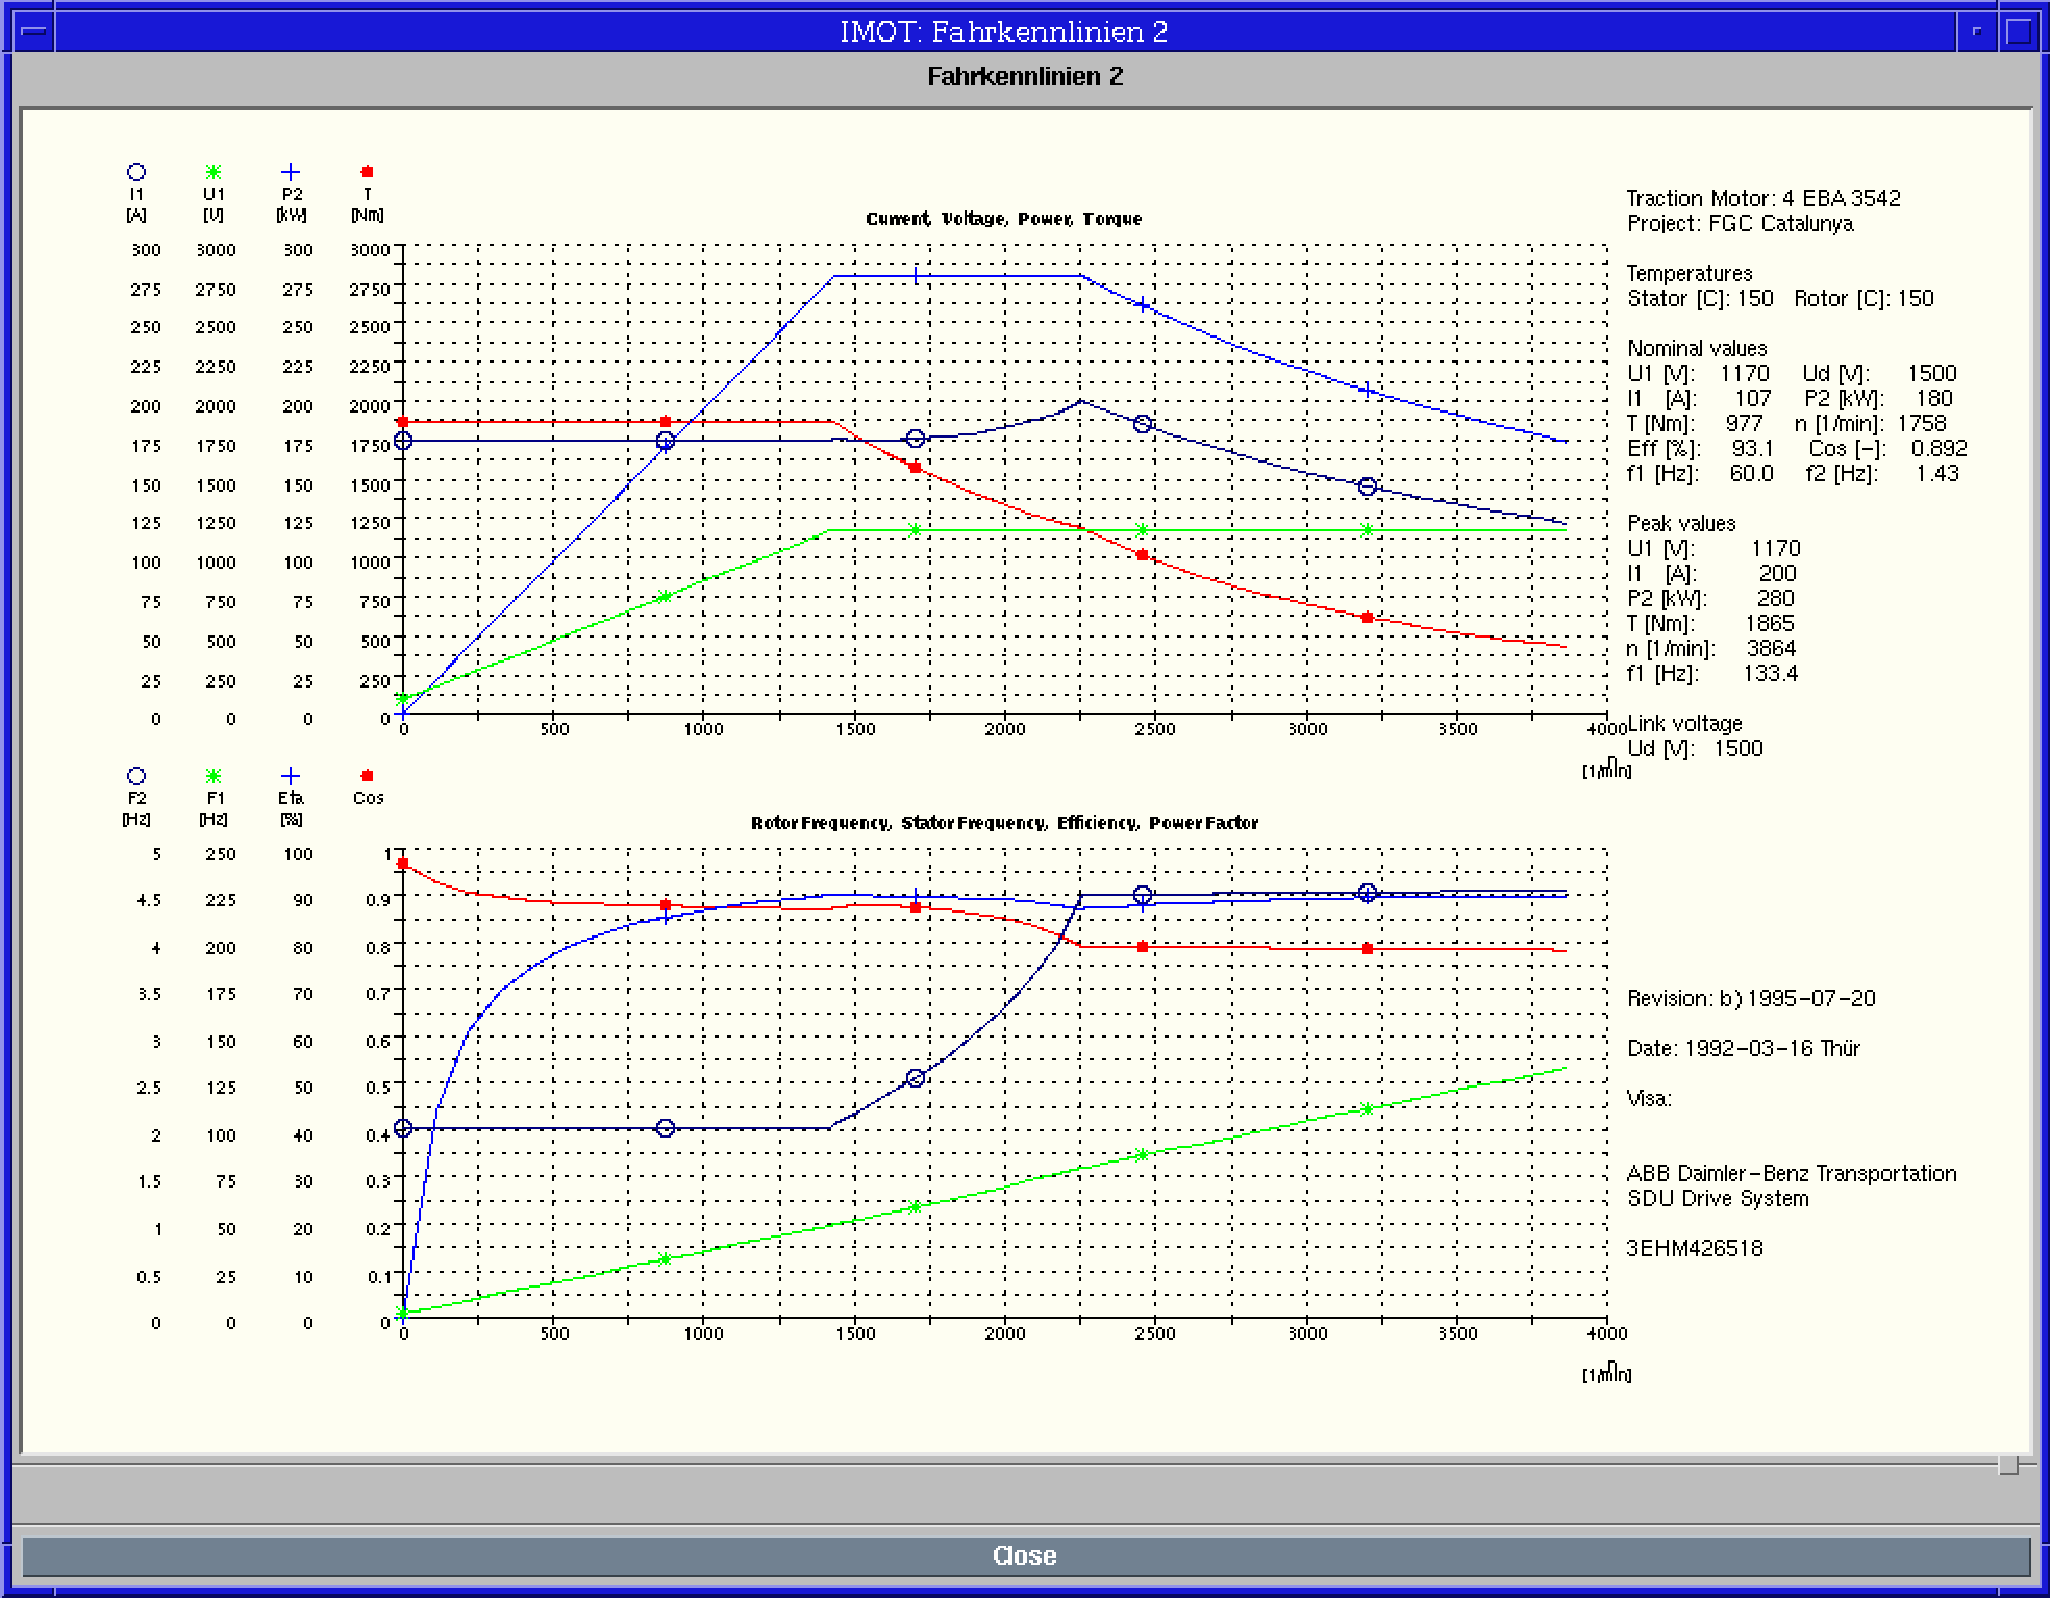
\includegraphics[width=\linewidth]{grab_listplot}
      \caption{\LISTPLOT{} diagram with 2 plots}
      \label{fig:listplot}
   \end{center}
\end{figure}

      %%%%%%%%%%%%%%%%%%%%%%%%%%%%%%%%%%%%%%%%%%%%%%%%%%%%%%%%%%%%%%%%%%%%%%%%%%%%%
%%%                                UNIPLOT                                %%%
%%%%%%%%%%%%%%%%%%%%%%%%%%%%%%%%%%%%%%%%%%%%%%%%%%%%%%%%%%%%%%%%%%%%%%%%%%%%%
\subsubsection{Uniplot}
\label{sec:uiuniplot}
\UNIPLOT{} is a ABB standard plot format with
\index{Plot!Uniplot}
a special set of plot vectors. It is mainly used within existing
Fortran programs. An example is given in figure \nameref{fig:uniplot}.

\input{diagrams/ui_uniplot_list}
\index{UNIPLOT@\UNIPLOT}
\index{PROCESSGROUP@\PROCESSGROUP!Uniplot}


\begin{boxedminipage}[t]{\linewidth}
\begin{intens}
DESCRIPTION "Example UNIPLOT";
  ... STUFF HERE ...
UI_MANAGER
  UNIPLOT
    mech_plot{ "Plot Mech" };
  FORM
    Form_Uniplot {"Plot Mech", HELPKEY "Mech_Plot", HIDECYCLE}
      ( ( mech_plot ) );
END UI_MANAGER;

OPERATOR
  PROCESS  plot_mech_proc : BATCH {"plotproc"};
  PROCESSGROUP
    mech_prog {"Mech"}(output_stream {DISPLAY=NONE},
                       mech_plot[mechuni] = plot_mech_proc( input_stream );
                     );
END OPERATOR;
  ... STUFF HERE ...
END.
\end{intens}
\end{boxedminipage}


%\newpage

\begin{figure}[h]
   \begin{center}
      \includegraphics[width=0.8\linewidth]{grab_uniplot}
   \end{center}
\caption{example of a UNIPLOT diagram}
  \label{fig:uniplot}
\end{figure}

      %%%%%%%%%%%%%%%%%%%%%%%%%%%%%%%%%%%%%%%%%%%%%%%%%%%%%%%%%%%%%%%%%%%%%%%%%%%%%
%%%                               PLOT3D                                  %%%
%%%%%%%%%%%%%%%%%%%%%%%%%%%%%%%%%%%%%%%%%%%%%%%%%%%%%%%%%%%%%%%%%%%%%%%%%%%%%
\subsubsection{Plot3D}
\label{sec:uiplot3d}
Plots of type \PLOTTHREED{} can be used to produce 3-dimensional graphs
of datapool values which have 2 dimensions.
\index{Plot!Plot3D}

\input{diagrams/ui_plot3d_list}
\index{PLOT3D@\PLOTTHREED}

Pressing the right mouse button within such a diagram pops up a menu which
provides additional configuration functions.

\input{diagrams/ui_plot3d_option}
\index{CAPTION@\CAPTION!3dplot option}
\index{STYLE@\STYLE!3dplot option}
\index{HIDDEN@\HIDDEN!3dplot option}
\index{SIZE@\SIZE!3dplot option}
\index{3DPLOT!CAPTION}
\index{3DPLOT!STYLE}
\index{3DPLOT!HIDDEN}
\index{3DPLOT!SIZE}


\begin{tabularx}{\textwidth}{l|X}
options       & description \\ \hline
\verb+string+ & defines the label string for the print menu button. \\
\CAPTION      & defines the caption text that will be printed at the bottom
                of the plot. The identifier must be a previously declared stream.
                (see section \nameref{sec:streamer} on page \pageref{sec:streamer})\\
\STYLE        & defines the initial style of the plot \\
\HIDDEN       & don't add the plot to the {\bfseries File Print} menu \\
\SIZE         & initial size in pixel \\
\end{tabularx}

\input{diagrams/ui_plot3d_style}
\index{BAR@\BAR!plot3d plotstyle}
\index{SURFACE@\SURFACE!plot3d plotstyle}
\index{CONTOUR@\CONTOUR!plot3d plotstyle}

\begin{tabularx}{\textwidth}{l|X}
style       & description \\
\hline
\BAR        & Draws bars \\
\SURFACE    & Fills in a color for each value. \\
\CONTOUR    & Does not fill in any color. \\
\end{tabularx}

\input{diagrams/ui_plot3d_graph}
\input{diagrams/ui_plot3d_graph_option_list}

\index{XAXIS@\XAXIS!plot3d graph option}
\index{YAXIS@\YAXIS!plot3d graph option}
\index{XANNOTATION@\XANNOTATION!plot3d graph option}
\index{YANNOTATION@\YANNOTATION!plot3d graph option}
\index{3DPLOT!XAXIS}
\index{3DPLOT!YAXIS}
\index{3DPLOT!XANNOTATION}
\index{3DPLOT!YANNOTATION}
\begin{tabularx}{\textwidth}{l|X}
graph options      & description \\ \hline
\verb+string+      & defines the plot3d graph title that will be printed at the top
                     of the plot.\\
\verb+identifier+  & defines the plot3d graph title that will be printed at the top
                     of the plot. The identifier must be a previously declared stream.
                     (see section \nameref{sec:streamer} on page \pageref{sec:streamer})\\
\XAXIS             & defines the x-coordinates\\
\YAXIS             & defines the y-coordinates\\
\XANNOTATION       & Shows x-axis as defined in plot3d-axis option \ANNOTATION{} on page \pageref{uiplot3daxisoption}. \\
\YANNOTATION       & Shows y-axis as defined in plot3d-axis option \ANNOTATION{} on page \pageref{uiplot3daxisoption}. \\
\end{tabularx}

\input{diagrams/ui_plot3d_graph_axis_item}
\input{diagrams/ui_plot3d_axis_option_list}
\input{diagrams/ui_plot3d_axis_option}
\label{uiplot3daxisoption}
\input{diagrams/ui_plot3d_axis_marker_option}
\input{diagrams/ui_plot3d_item}

\index{Scale factors!plot3d item}
\index{LABEL@\LABEL!plot3d}
\index{SCALE@\SCALE!plot3d}
\index{ANNOTATION@\ANNOTATION!plot3d}
\index{MARKER@\MARKER!plot3d}
\index{3DPLOT!LABEL}
\index{3DPLOT!SCALE}
\index{3DPLOT!ANNOTATION}
\index{3DPLOT!MARKER}
\begin{tabularx}{\textwidth}{l|X}
plot item option & description \\ \hline
\verb+scale+     & see section \nameref{sec:scale} page \pageref{sec:scale}. \\
\LABEL           & defines the label that will be printed at the top of the axis\\
\SCALE           & axis scale (min, max) \\
\ANNOTATION      & defines extra labels for the axis (see page \pageref{uixrtgraphitemoptionsxannotation}).\\
\MARKER          & show markers with optional labels \\

\end{tabularx}


\begin{boxedminipage}[t]{\linewidth}
\begin{alltt}
\DESCRIPTION "Example 3D PLOT";
\DATAPOOL
  \REAL \{\EDITABLE\}
    matrix
   ,xValues
   ,yValues
   ;
\END \DATAPOOL;

\UIMANAGER
  \PLOTTHREED
    plot_3d
      \{ \CAPTION = "streamCaption" \}
      ( plot
           \{ "SIN(x) * COS(y)"
           , \XAXIS = xValues \{ \LABEL = "X-Axis" \}
           , \YAXIS = yValues \{ \LABEL = "Y-Axis" \}
           \}
         ( matrix * 0.01 \{ \LABEL = "Matrix Values" \}
         )
      );
  \FORM
    Form_Plot3D \{"3D Plot", \HIDECYCLE\}
      ( ( plot_3d )
      );
\END \UIMANAGER;
\END.
\end{alltt}
\end{boxedminipage}


%
\newpage

%
\begin{figure}[h]\label{fig:plot3dPlotStyles}
  \begin{center}
    {\LARGE PLOT3D Plot styles \\[2ex]}
    \begin{minipage}{0.45\linewidth}
      \begin{center}
        \index{PLOT3D@\PLOTTHREED!plot style example!bar}
        \includegraphics[width=0.8\linewidth]{plot3d-style_bar}
        \label{hc:plot3d_style_bar}
      \end{center}
    \end{minipage} \\[3ex]

    \begin{minipage}{0.45\linewidth}
      \begin{center}
        \index{PLOT3D@\PLOTTHREED!plot style example!surface}
        \includegraphics[width=0.8\linewidth]{3dplot-style_surface}
        \label{hc:plot3d_style_surface}
      \end{center}
    \end{minipage} \\[3ex]

    \begin{minipage}{0.45\linewidth}
      \begin{center}
        \index{PLOT3D@\PLOTTHREED!plot style example!contour}
        \includegraphics[width=0.8\linewidth]{plot3d-style_contour}
        \label{hc:plot3d_style_contour}
      \end{center}
    \end{minipage}
  \end{center}
  \caption{PLOT3D Plot styles}
\end{figure}

%      %%%%%%%%%%%%%%%%%%%%%%%%%%%%%%%%%%%%%%%%%%%%%%%%%%%%%%%%%%%%%%%%%%%%%%%%%%%%%
%%%                               XRTGRAPH                                %%%
%%%%%%%%%%%%%%%%%%%%%%%%%%%%%%%%%%%%%%%%%%%%%%%%%%%%%%%%%%%%%%%%%%%%%%%%%%%%%
\subsubsection{XrtGraph}
\label{sec:uixrtgraph}
Plots of type \XRTGRAPH{} can be used to produce 2-dimensional graphs
of datapool values.
\index{Plot!XrtGraph}

\input{diagrams/ui_xrtgraph_list}
\index{XRTGRAPH@\XRTGRAPH}

Pressing the right mouse button within such a diagram pops up a menu which
provides additional configuration functions.

\label{uixrtgraphoptions}
\input{diagrams/ui_xrtgraph_option}

\index{CAPTION@\CAPTION!xrtgraph option}
\index{PRINTSTYLE@\PRINTSTYLE!xrtgraph option}
\index{TRUE@\TRUE!xrtgraph option printstyle}
\index{XRTGRAPH@\XRTGRAPH!CAPTION}
\begin{tabularx}{\textwidth}{l|X}
options          & description \\ 
\hline
string           & Print-menu label \\
\CAPTION         & Titel displayed at the bottom of the graphics-form. \\
                 & Using special-characters such as space, you need to use string-representation. \\
\PRINTSTYLE      & = TRUE use extra resources for printing (fonts, line styles, background etc.). \\
\MINMAX          & show(TRUE, default) or hide (FALSE) min and max of a selected curve. \\
\RMS             & show(TRUE, default) or hide (FALSE) rms of a selected curve. \\
\AVG             & show(TRUE, default) or hide (FALSE) avg and max of a selected curve. \\

\end{tabularx}
\newpage

\input{diagrams/ui_xrtgraph_graph}
\input{diagrams/ui_xrtgraph_graph_option}
\input{diagrams/ui_xrtgraph_graph_axis_item}

\index{XAXIS@\XAXIS!xrtgraph graph option}
\index{YAXIS1@\YAXISONE!xrtgraph graph option}
\index{YAXIS2@\YAXISTWO!xrtgraph graph option}
\index{AXES\_ORIGIN\_X@\AXESORIGINX!xrtgraph graph option}
\index{AXES\_ORIGIN\_Y@\AXESORIGINY!xrtgraph graph option}
\index{LOG\_X@\LOGX!xrtgraph graph option}
\index{LOG\_Y@\LOGY!xrtgraph graph option}
\index{XANNOTATION@\XANNOTATION!xrtgraph graph option}
\begin{tabularx}{\textwidth}{l|X}
graph options      & description \\
\hline
\verb+string+      & defines the xrt graph title that will be printed at the top
                     of the plot.\\
\verb+identifier+  & defines the xrt3d graph title that will be printed at the top
                     of the plot. The identifier must be a previously declared stream.
                     (see section \nameref{sec:streamer} on page \pageref{sec:streamer})\\
\XAXIS             & defines the x-coordinates\\
\YAXISONE          & defines coordinates of first Y-Axis\\
\YAXISTWO          & defines coordinates of second Y-Axis\\
\AXESORIGINX       & defines the origin for the x axis\\
\AXESORIGINY       & defines the origin for all y axes\\
\LOGX              & the x-axis is scaled logarithmically\\
\LOGY              & the y-axis is scaled logarithmically\\
\COMBOBOX          & displays the item names as a combobox when the config menu
                          is opened pressing the right mouse button over the plot. \\
\STYLE             & style of all curves. \\
\YONESTYLE         & style of y1 curves. \\
\YTWOSTYLE         & style of y2 curves. \\
\ALLCYCLES         & Shows data of each cylcle in same graph. \\
\SCROLLBARS        & Shows scroll-bars in 'zoomed zone' mode. \\
\XANNOTATION       & Shows x-axis as defined in x-graph-item option XANNOTATION on page
                        \pageref{uixrtgraphitemoptions}. \\
\end{tabularx}

\input{diagrams/ui_xrtgraph_xaxis_label}
\input{diagrams/ui_xrtgraph_yaxis1_label}

\begin{tabularx}{\textwidth}{l|X}
axis-options & description \\
\hline
\LABEL       & Text to display for describing the axis. \\
\end{tabularx}

\input{diagrams/ui_xrtgraph_style}

\begin{tabularx}{\textwidth}{l|X}
plot styles        & description \\
\hline
\BAR               & see hardcopy example on page \pageref{hc:plot2d_style_bar} \\
\AREA              & see hardcopy example on page \pageref{hc:plot2d_style_area} \\
\PLOT              & see hardcopy example on page \pageref{hc:plot2d_style_plot} \\
\POLAR             & see hardcopy example on page \pageref{hc:plot2d_style_polar} \\
\STACKINGBAR       & see hardcopy example on page \pageref{hc:plot2d_style_stacking_bar} \\
\STEP              & see hardcopy example on page \pageref{hc:plot2d_style_step} \\
\end{tabularx}

\input{diagrams/ui_xrtgraph_item}

\index{scale}
\begin{tabularx}{\textwidth}{l|X}
2d item list & description \\
\hline
\verb+scale+ & see section \nameref{sec:scale} page \pageref{sec:scale}. \\
\end{tabularx}

\input{diagrams/ui_xrtgraph_item_option}
\label{uixrtgraphitemoptions}
\index{LABEL@\LABEL!xrtgraph item option}
\index{UNIT@\UNIT!xrtgraph item option}
\index{YAXIS1@\YAXISONE!xrtgraph item option}
\index{YAXIS2@\YAXISTWO!xrtgraph item option}
\index{XAXIS@\XAXIS!xrtgraph item option}
\index{HIDDEN@\HIDDEN!xrtgraph item option}
\index{XANNOTATION@\XANNOTATION!xrtgraph item option}
\index{LINESTYLE@\LINESTYLE!xrtgraph item option}
\index{LINEAR@\LINEAR!xrtgraph item option}
\index{STEP@\STEP!xrtgraph item option}


\begin{tabularx}{\textwidth}{l|X}
graph item options & description \\ 
\hline
\LABEL        & defines the item name which will be printed at the top of the axis\\
\UNIT         & defines the unit description which will be printed at the top of the axis\\
\YAXISONE     & defines the y-coordinates of the left y axis\\
\YAXISTWO     & defines the y-coordinates of the right y axis\\
\XAXIS        & defines the coordinates of the x axis\\
\HIDDEN       & does not print any description at the top of the axis\\
\XANNOTATION  & defines extra labels for x axis\\
\LINESTYLE    & defines the line style \\
\LINEAR       & TODO \\
\STEP         & TODO \\
\end{tabularx}

\input{diagrams/ui_xrtgraph_item_anno}
\input{diagrams/ui_xrtgraph_item_anno_title}
\input{diagrams/ui_xrtgraph_item_anno_values}
\input{diagrams/ui_xrtgraph_item_anno_labels}
\input{diagrams/ui_xrtgraph_item_anno_angle}
\label{uixrtgraphitemoptionsxannotation}

\index{LABEL@\LABEL!xrtgraph option!xannotation}
\index{XANNOTATION@\XANNOTATION!xrtgraph x graph option}
\index{Scale factors!xrtgraph xannotation}
\begin{tabularx}{\textwidth}{l|X}
graph item options & description \\ 
\hline
\LABEL             & title which will be printed at the bottom of graphics \\
\verb+anno values+ & {\bfseries data item}: position on the x axis, where labels will be displayed.\\
\verb+scale+       & scale factor (see section \nameref{sec:scale} page \pageref{sec:scale}). \\
\verb+anno labels+ & {\bfseries string data item}: labels to be displayed at display position.\\
\verb+anno angle+  & angle (in degrees) to print the labels. Default is 90 (vertical). 0 is horizontal. \\
\end{tabularx}


\begin{boxedminipage}[t]{\linewidth}
\begin{alltt}
\DESCRIPTION "Example XRTGRAPH";
\DATAPOOL
  \REAL \{\EDITABLE\}
    xValues
   ,y1Values
   ,y2Values
   ;
\END \DATAPOOL;

\UIMANAGER
  \XRTGRAPH
    graph_plot
      \{ \CAPTION = streamCaption \}
      ( plot
           \{ streamTitel
           , \XAXIS = xValues \{ \LABEL = "X-Axis" \}
           \}
         (
           xValues,
           y1Values \{\YAXISONE\},
           y2Values \{\YAXISTWO\}
         )
      );
  \FORM
    Form_XrtGraph \{"Graph Plot", \HIDECYCLE\}
      ( ( graph_plot )
      );
\END \UIMANAGER;
\END.
\end{alltt}
\end{boxedminipage}


      %%%%%%%%%%%%%%%%%%%%%%%%%%%%%%%%%%%%%%%%%%%%%%%%%%%%%%%%%%%%%%%%%%%%%%%%%%%%%
%%%                               PLOT2D                                  %%%
%%%%%%%%%%%%%%%%%%%%%%%%%%%%%%%%%%%%%%%%%%%%%%%%%%%%%%%%%%%%%%%%%%%%%%%%%%%%%
\subsubsection{Plot2d}
\label{sec:uiplot2d}
Plots of type \PLOTTWOD{} can be used to produce 2-dimensional graphs of datapool values.
\index{PLOT2D@\PLOTTWOD}
\index{Plot!Plot2d}

\input{diagrams/ui_plot2d_list}
\index{XRTGRAPH@\XRTGRAPH!use \PLOTTWOD}

Pressing the right mouse button within such a diagram pops up a menu which
provides additional configuration functions.
See \nameref{dia:uiplot2dmenuentrylist} on page \pageref{dia:uiplot2dmenuentrylist}.

\paragraph{UI Mode}
\label{par:uiplot2duimode}
\index{PLOT2D@\PLOTTWOD!UI Mode}
\index{PLOT2D\_UIMODE@\PLOTTWODUIMODE!predefined datapool item}
One option in that menu is the UI Mode. The UI Mode defines the behaviour
of the left mouse button inside the plot2ds.

The mode can be changed using
\begin{itemize}
  \item that menu
  \item keyboard shortcuts (when focus is on a \PLOTTWOD)
  \item \DATAPOOL{} variable \PLOTTWODUIMODE
\end{itemize}

The first two ways automatically change the value of \PLOTTWODUIMODE{}.

All \PLOTTWOD{}s within one application share one global UI Mode.
The following modes exist:

\begin{tabularx}{\textwidth}{p{4cm}|X}
UI Mode           & Shortcut (hint) \PLOTTWODUIMODE{} value \newline
                    description \\
\hline
Zoom              &  Ctrl-S (scale) ``ZOOM'' \newline
                     Select a rectangle to zoom in. \\
Select Point      & Ctrl-D (dot) ``SELECT\_POINT'' \newline
                    Select a point (not a line) of a plot curve. \newline
                    If the plot2d has the \FUNC{} option, that function is called
                    and \REASONSELECTPOINT{} is set. \INDEX{} is set to the index
                    of the selected point.
                    The function can access the coordinates of the point using the datapool variables
                    Global\_Point.X and Global\_Point.Y. \newline
                    Without the \FUNC{} option, you can select multiple points.
                    Select the same point again to unselect it. Use \GETSELECTION{} in a function
                    to get the information about the selected points.
                    See \nameref{dia:guimorestatement} on page \pageref{dia:guimorestatement}. \\
Select Rectangle  & Ctrl-A (area) ``SELECT\_RECTANGLE'' \newline
                    This mode is only available when the \FUNC{} option is set.
                    That function is called after selecting a rectangle and \REASONSELECTRECTANGLE{} is set.
                    The function can access the coordinates of the rectangle using the datapool variables
                    Global\_Rect.X1,  Global\_Rect.X2, Global\_Rect.Y1 and Global\_Rect.Y1. \\
\end{tabularx}
\vspace{0.5cm}

\paragraph{Global Symbolsize}
\label{par:uiplot2symbolsize}
\index{PLOT2D@\PLOTTWOD!Global Symbolsize}
\index{PLOT2D\_SYMBOLSIZE@\PLOTTWODSYMBOLSIZE!predefined datapool item}
The symbol sizes of \PLOTTWOD{} curves are normally defined in the resource file.
The user can change them using the option Configuration... in the right mouse button menu of a \PLOTTWOD.

And the symbol size of all \PLOTTWOD{} can be changed to the same value using
the \DATAPOOL{} variable \PLOTTWODSYMBOLSIZE{}. When that variable has a value,
it is used. When the value is cleared, the \PLOTTWOD{}s use the configured symbol sizes again.


\label{uiplot2doptions}
\input{diagrams/ui_plot2d_option}

\index{CAPTION@\CAPTION!plot2d option}
\index{PRINTSTYLE@\PRINTSTYLE!plot2d option}
\index{TRUE@\TRUE!plot2d option printstyle}
\index{HIDDEN@\HIDDEN!plot2d option}
\index{MINMAX@\MINMAX!plot2d option}
\index{RMS@\RMS!plot2d option}
\index{AVG@\AVG!plot2d option}
\index{PLOT2D@\PLOTTWOD!CAPTION@\CAPTION}
\index{PLOT2D@\PLOTTWOD!PRINTSTYLE@\PRINTSTYLE}
\index{PLOT2D@\PLOTTWOD!HIDDEN@\HIDDEN}
\index{PLOT2D@\PLOTTWOD!MINMAX@\MINMAX}
\index{PLOT2D@\PLOTTWOD!RMS@\RMS}
\index{PLOT2D@\PLOTTWOD!AVG@\AVG}
\begin{tabularx}{\textwidth}{l|X}
options     & description \\
\hline
string      & Menutext \\
\CAPTION    & Footertext: Title displayed in the graphics-form. (Using special-characters such as space, you need to use string-representation.) \newline
              identifier may also refere to a previously declared stream. \\
\PRINTSTYLE & = \TRUE{} prints out graph descriptions. Use extra resources for printing (fonts, line styles, background etc.). \\
\HIDDEN     & don't add the plot to the {\bfseries File Print} menu \\
\MINMAX     & show(\TRUE, default) or hide (\FALSE) min and max of a selected curve. \\
\RMS        & show(\TRUE, default) or hide (\FALSE) rms of a selected curve. \\
\AVG        & show(\TRUE, default) or hide (\FALSE) avg and max of a selected curve. \\
\end{tabularx}


\input{diagrams/ui_plot2d_graph}
\input{diagrams/ui_plot2d_item_list}
\input{diagrams/ui_plot2d_graph_option}

\index{XAXIS@\XAXIS!plot2d graph option}
\index{XAXIS2@\XAXISTWO!plot2d graph option}
\index{YAXIS1@\YAXISONE!plot2d graph option}
\index{YAXIS2@\YAXISTWO!plot2d graph option}
\index{SIZE@\SIZE!plot2d graph option}
\index{AXES\_ORIGIN\_X@\AXESORIGINX!plot2d graph option}
\index{AXES\_ORIGIN\_Y@\AXESORIGINY!plot2d graph option}
\index{LOG\_X@\LOGX!plot2d graph option}
\index{LOG\_Y@\LOGY!plot2d graph option}
\index{COMBOBOX@\COMBOBOX!plot2d graph option}
\index{STYLE@\STYLE!plot2d graph option}
\index{Y1\_STYLE@\YONESTYLE!plot2d graph option}
\index{Y2\_STYLE@\YTWOSTYLE!plot2d graph option}
\index{ALLCYCLES@\ALLCYCLES!plot2d graph option}
\index{SCROLLBARS@\SCROLLBARS!plot2d graph option}
\index{XANNOTATION@\XANNOTATION!plot2d graph option}
\index{FUNC@\FUNC!plot2d graph option}
\index{COLOR@\COLOR!plot2d graph option}
\index{PLOT2D@\PLOTTWOD!XAXIS@\XAXIS}
\index{PLOT2D@\PLOTTWOD!XAXIS2@\XAXISTWO}
\index{PLOT2D@\PLOTTWOD!YAXIS1@\YAXISONE}
\index{PLOT2D@\PLOTTWOD!YAXIS2@\YAXISTWO}
\index{PLOT2D@\PLOTTWOD!SIZE@\SIZE}
\index{PLOT2D@\PLOTTWOD!AXES\_ORIGIN\_X@\AXESORIGINX}
\index{PLOT2D@\PLOTTWOD!AXES\_ORIGIN\_Y@\AXESORIGINY}
\index{PLOT2D@\PLOTTWOD!LOG\_X@\LOGX}
\index{PLOT2D@\PLOTTWOD!LOG\_Y@\LOGY}
\index{PLOT2D@\PLOTTWOD!COMBOBOX@\COMBOBOX}
\index{PLOT2D@\PLOTTWOD!STYLE@\STYLE}
\index{PLOT2D@\PLOTTWOD!Y1\_STYLE@\YONESTYLE}
\index{PLOT2D@\PLOTTWOD!Y2\_STYLE@\YTWOSTYLE}
\index{PLOT2D@\PLOTTWOD!ALLCYCLES@\ALLCYCLES}
\index{PLOT2D@\PLOTTWOD!SCROLLBARS@\SCROLLBARS}
\index{PLOT2D@\PLOTTWOD!XANNOTATION@\XANNOTATION}
\index{PLOT2D@\PLOTTWOD!FUNC@\FUNC}
\index{PLOT2D@\PLOTTWOD!COLOR@\COLOR}
\begin{tabularx}{\textwidth}{l|X}
2d graph options       & description \\
\hline
\verb+string+         & defines the graph title that will be printed at the top of the plot.\\
{\bfseries ID\_STREAM} & defines the graph title that will be printed at the top of the plot. The identifier must be a previously declared stream. (see section \nameref{sec:streamer} on page \pageref{sec:streamer}) \\
\XAXIS \{..\}          & describes the x-axis. \\
\XAXISTWO \{..\}       & describes the x2-axis. This only draws an axis on top of the plot with the given \SCALE.
                         Without \SCALE, this option does not make sense. \\
\YAXISONE \{..\}         & describes the y1-axis. \\
\YAXISTWO \{..\}         & describes the y2-axis. \\
\AXESORIGINX           & defines the origin for the x-axis. \\
\AXESORIGINY           & defines the origin for all y-axis. \\
\LOGX                  & the x-axis is scaled logarithmically. \\
\LOGY                  & the y-axis is scaled logarithmically. \\
\COMBOBOX              & displays the item names as a combobox when the config menu is opened pressing the right mouse button over the plot. \\
\STYLE                 & style of all curves. \\
\YONESTYLE             & style of y1 curves. \\
\YTWOSTYLE             & style of y2 curves. \\
\ALLCYCLES             & Shows data of each cylcle in same graph. \\
\SCROLLBARS            & Shows scroll-bars in 'zoomed zone' mode. \\
\XANNOTATION           & Shows x-axis as defined in x-graph-item option \XANNOTATION{} on page \pageref{uiplot2dxitemoptions}. \\
\FUNC                  & Defines the function that will be called when a point or rectangle is selected.
                         See paragraph \nameref{par:uiplot2duimode} in section \nameref{sec:uiplot2d} on page \pageref{par:uiplot2duimode}.\\
\COLOR{} = ...         & Defines the color set that will be used for the colors of the plot curves.
                         See section \nameref{sec:dpcolorset} on page \pageref{sec:dpcolorset}.\\
\end{tabularx}

\input{diagrams/ui_plot2d_xaxis_options}
\index{LABEL@\LABEL!plot2d option!axis}
\index{SCALE@\SCALE!plot2d option!axis}
\index{FORMAT@\FORMAT!plot2d option!axis}
\index{HIDDEN@\HIDDEN!plot2d option!axis}
\index{ASPECT\_RATIO\_REF\_AXIS@\ASPECTRATIOREFAXIS!plot2d option!axis}
\index{ASPECT\_RATIO@\ASPECTRATIO!plot2d option!axis}
\index{PLOT2D@\PLOTTWOD!LABEL@\LABEL}
\index{PLOT2D@\PLOTTWOD!SCALE@\SCALE}
\index{PLOT2D@\PLOTTWOD!FORMAT@\FORMAT}
\index{PLOT2D@\PLOTTWOD!HIDDEN@\HIDDEN}
\index{PLOT2D@\PLOTTWOD!ASPECT\_RATIO\_REF\_AXIS@\ASPECTRATIOREFAXIS}
\index{PLOT2D@\PLOTTWOD!ASPECT\_RATIO@\ASPECTRATIO}

\begin{tabularx}{\textwidth}{l|X}
2d axis options  & description \\
\hline
\LABEL           & axis label \\
\SCALE           & axis scale (min, max) \\
\FORMAT          & axis label number format: width[:precision] \newline
                   ``10'' : width of the number \newline
                   ``10:2'' : width and decimals of the number \\
\HIDDEN          & hide the axis labels \\
\ASPECTRATIOREFAXIS & This axis is the reference axis for calculating the unit scaling of the plot.
                      The length (in pixel) and axis range of this axis is the reference for the other axis.
                      The length of the other axis is adapted to get the desired unit scaling. \newline
                      Define \ASPECTRATIO{} for both axes. \newline
                      See example on page \pageref{des:plot2dAspectRatio} and
                      hardcopy example on page \pageref{hc:plot2dAspectRatio}. \\
\ASPECTRATIO     & The meaning of this option differs for the reference axis (with \ASPECTRATIOREFAXIS)
                   and the other axis: \newline
                   {\bfseries Reference axis}: Range of the reference axis relative to the other axis.
                   As this axis is the reference axis, the range of the other axis is calculated as
                   (range reference axis / this factor). \newline
                   Example: Reference axis range: 0 .. 250 = 250. \newline
                   ~ 2: range of the other axis is 250 / 2 = 125. \newline
                   ~ 0.5: range of the other axis is 250 / 0.5 = 500. \newline
                   {\bfseries Other axis}: Defines the unit scaling (pixel per unit) of this axis
                   relative to the reference axis. \newline
                   Examples: \newline
                   ~ 1: same unit scaling as the reference axis. \newline
                   ~ 2: 1 unit on this axis needs twice the pixels as on the reference axis. \newline
                   ~ 0.5: 1 unit on this axis needs half the pixels as on the reference axis. \newline
                   See example on page \pageref{des:plot2dAspectRatio} and
                   hardcopy example on page \pageref{hc:plot2dAspectRatio}. \\
\end{tabularx}

\newpage

\input{diagrams/ui_plot2d_style}

\index{BAR@\BAR!plot2d plotstyle}
\index{AREA@\AREA!plot2d plotstyle}
\index{PLOT@\PLOT!plot2d plotstyle}
\index{POLAR@\POLAR!plot2d plotstyle}
\index{STACKING\_BAR@\STACKINGBAR!plot2d plotstyle}
\index{STEP@\STEP!plot2d plotstyle}
\index{PLOT2D@\PLOTTWOD!plot styles}
\index{PLOT2D@\PLOTTWOD!plot styles!BAR@\BAR}
\index{PLOT2D@\PLOTTWOD!plot styles!AREA@\AREA}
\index{PLOT2D@\PLOTTWOD!plot styles!PLOT@\PLOT}
\index{PLOT2D@\PLOTTWOD!plot styles!POLAR@\POLAR}
\index{PLOT2D@\PLOTTWOD!plot styles!STACKING\_BAR@\STACKINGBAR}
\index{PLOT2D@\PLOTTWOD!plot styles!STEP@\STEP}
\begin{tabularx}{\textwidth}{l|X}
plot style    & description \\
\hline
\PLOT        & see hardcopy example on page \pageref{hc:plot2d_style_plot} \\
\BAR          & see hardcopy example on page \pageref{hc:plot2d_style_bar} \\
\STACKINGBAR  & see hardcopy example on page \pageref{hc:plot2d_style_stacking_bar} \\
\AREA         & see hardcopy example on page \pageref{hc:plot2d_style_area} \\
\POLAR        & see hardcopy example on page \pageref{hc:plot2d_style_polar} \\
\STEP         & see hardcopy example on page \pageref{hc:plot2d_style_step} \\
\DOTS         & show a symbol at every data point \\
\end{tabularx}

\input{diagrams/ui_plot2d_item}

\input{diagrams/ui_plot2d_x_item}

\index{Scale factors!plot2d item}
\begin{tabularx}{\textwidth}{l|X}
2d item list & description \\
\hline
\verb+scale+ & see section \nameref{sec:scale} page \pageref{sec:scale}. \\
\end{tabularx}

\input{diagrams/ui_plot2d_x_item_option}
\label{uiplot2dxitemoptions}

\index{LABEL@\LABEL!plot2d option!x graph}
\index{UNIT@\UNIT!plot2d option!x graph}
\index{XANNOTATION@\XANNOTATION!plot2d graph item option}
\index{INDEX@\INDEX!plot2d graph item option}
\index{XAXIS@\XAXIS!plot2d graph item option}
\index{PLOT2D@\PLOTTWOD!LABEL@\LABEL}
\index{PLOT2D@\PLOTTWOD!UNIT@\UNIT}
\index{PLOT2D@\PLOTTWOD!XANNOTATION@\XANNOTATION}
\index{PLOT2D@\PLOTTWOD!INDEX@\INDEX}
\index{PLOT2D@\PLOTTWOD!XAXIS@\XAXIS}
\begin{tabularx}{\textwidth}{l|X}
X-graph item option & description \\
\hline
\verb+string+      & title which will be printed to the right of x-axis description. \\
\LABEL              & defines the item name which will be printed as the x-axis description. \newline
                      use a \STREAM{} when the name needs to be variable. \\
\UNIT               & defines the unit description which will be printed to the right of x-axis description. \\
\XANNOTATION        & defines extra labels for x axis (see page \pageref{uixrtgraphitemoptionsxannotation}).\\
\INDEX              & Data reference has two wildcards. One (defined here) is used to create many curves. \\
\XAXIS              & defines the x-coordinates of the x-axis. \\

\end{tabularx}

\input{diagrams/ui_plot2d_y_item}

\index{Scale factors!plot2d y item}
\begin{tabularx}{\textwidth}{l|X}
y item list  & description \\
\hline
\verb+scale+ & see section \nameref{sec:scale} page \pageref{sec:scale}. \\
\end{tabularx}

\input{diagrams/ui_plot2d_y_item_option}

\index{YAXIS1@\YAXISONE!plot2d y graph option}
\index{YAXIS2@\YAXISTWO!plot2d y graph option}
\index{LABEL@\LABEL!plot2d option!y graph}
\index{UNIT@\UNIT!plot2d option!y graph}
\index{HIDDEN@\HIDDEN!plot2d graph item option}
\index{MARKER@\MARKER!plot2d graph item option}
\index{COLOR@\COLOR!plot2d graph item option}
\index{INDEX@\INDEX!plot2d graph item option}
\index{LEGEND@\LEGEND!plot2d graph item option}
\index{XANNOTATION@\XANNOTATION!plot2d graph item option}
\index{XAXIS@\XAXIS!plot2d graph item option}
\index{PLOT2D@\PLOTTWOD!YAXIS1@\YAXISONE}
\index{PLOT2D@\PLOTTWOD!YAXIS2@\YAXISTWO}
\index{PLOT2D@\PLOTTWOD!LABEL@\LABEL}
\index{PLOT2D@\PLOTTWOD!UNIT@\UNIT}
\index{PLOT2D@\PLOTTWOD!HIDDEN@\HIDDEN}
\index{PLOT2D@\PLOTTWOD!MARKER@\MARKER}
\index{PLOT2D@\PLOTTWOD!COLOR@\COLOR}
\index{PLOT2D@\PLOTTWOD!INDEX@\INDEX}
\index{PLOT2D@\PLOTTWOD!LEGEND@\LEGEND}
\index{PLOT2D@\PLOTTWOD!XANNOTATION@\XANNOTATION}
\index{PLOT2D@\PLOTTWOD!XAXIS@\XAXIS}
\begin{tabularx}{\textwidth}{l|X}
Y-graph item option & description \\
\hline
\verb+string+      & title which will be printed at the top of the plot. \\
\YAXISONE           & defines the y-coordinates of the left y-axis. \\
                    & If this option is omited, the axis is not displayed at startup. \\
\YAXISTWO           & defines the y-coordinates of the right y-axis. \\
                    & If this option is omited, the axis is not displayed at startup. \\
\LABEL              & defines the item name which is used in the plot legend. \newline
                      use a \STREAM{} when the name needs to be variable. \\
\UNIT               & defines the unit description which will be printed at the top of the axis. \\
\HIDDEN             & does not display the axis. \\
\MARKER             & show markers with optional labels \\
\COLOR{} = ...      & use a color set (see section \nameref{sec:dpcolorset} on page \pageref{sec:dpcolorset})
                      to show the markers in different colors.
                      The provided marker labels are the values used to get a color from the color set. \\
\INDEX              & Data reference has two wildcards. One (defined here) is used to create many curves. \\
\LEGEND             & show (\TRUE, default) or hide (\FALSE) this curve in the legend \\
\XAXIS              & defines the x-coordinates of the x-axis. \\
\XANNOTATION        & defines extra labels for x axis (see page \pageref{uixrtgraphitemoptionsxannotation}).\\
\end{tabularx}


% PLOT2D Examples (Styles)
%%%%%%%%%%%%%%%%%%%%%%%%%%%%%%%%%%%%%%%%%%%%%%%%%%%%%%%%%%%%%%%%%%%%%%%%%%%%%
\index{PLOT2D@\PLOTTWOD!example!STYLE@\STYLE}

\begin{boxedminipage}[t]{\linewidth}
\begin{alltt}
\DESCRIPTION "Example PLOT-2D";
\DATAPOOL
  \REAL \{\EDITABLE\}
    xValues,
    y1Values,
    y2Values
  ;
\END \DATAPOOL;

\STREAMER
  streamer_identifier ("Plot Title");
\END \STREAMER;

\UIMANAGER
  \PLOTTWOD
    plot2d_identifier
    (
      graph_identifier \{streamer_identifier\}
      (
        xValues \{\LABEL="x-axis"\}
        (
          y1Values \{\YAXISONE, \LABEL="y1-axis"\},
          y2Values \{\YAXISONE, \LABEL="y2-axis"\}
        )
      )
    )
  ;
  \FORM
    form_identifier \{"2D Plot", \HIDECYCLE\}
    (
      ( plot2d_identifier )
    )
  ;
\END \UIMANAGER;
\END.
\end{alltt}
\end{boxedminipage}

%
\newpage

\begin{figure}[H]\label{fig:plot2dPlotStyles}
  \begin{center}
    {\LARGE Plot styles \\[2ex]}
    %
    \begin{minipage}{0.45\linewidth}
      \begin{center}
        \index{PLOT2D@\PLOTTWOD!plot styles!BAR@\BAR}
        \includegraphics[width=0.8\linewidth]{plot2d-styles_bar}
        \label{hc:plot2d_style_bar}
      \end{center}
    \end{minipage}
    \hfill
    \begin{minipage}{0.45\linewidth}
      \begin{center}
        \index{PLOT2D@\PLOTTWOD!plot styles!AREA@\AREA}
        \includegraphics[width=0.8\linewidth]{plot2d-styles_area}
        \label{hc:plot2d_style_area}
      \end{center}
    \end{minipage}\\[3ex]
    %
    \begin{minipage}{0.45\linewidth}
      \begin{center}
        \index{PLOT2D@\PLOTTWOD!plot styles!PLOT@\PLOT}
        \includegraphics[width=0.8\linewidth]{plot2d-styles_plot}
        \label{hc:plot2d_style_plot}
      \end{center}
    \end{minipage}
    \hfill
    \begin{minipage}{0.45\linewidth}
      \begin{center}
        \index{PLOT2D@\PLOTTWOD!plot styles!POLAR@\POLAR}
        \includegraphics[width=0.8\linewidth]{plot2d-styles_polar}
        \label{hc:plot2d_style_polar}
      \end{center}
    \end{minipage}\\[3ex]
    %
    \begin{minipage}{0.45\linewidth}
      \begin{center}
        \index{PLOT2D@\PLOTTWOD!plot styles!STACKING\_BAR@\BAR}
        \includegraphics[width=0.8\linewidth]{plot2d-styles_stacking_bar}
        \label{hc:plot2d_style_stacking_bar}
      \end{center}
    \end{minipage}
    \hfill
    \begin{minipage}{0.45\linewidth}
      \begin{center}
        \index{PLOT2D@\PLOTTWOD!plot styles!STEP@\STEP}
        \includegraphics[width=0.8\linewidth]{plot2d-styles_step}
        \label{hc:plot2d_style_step}
      \end{center}
    \end{minipage}
  \end{center}
  \caption{Plot2d Plot styles}
\end{figure}
%
\newpage

% PLOT2D Example ASPECT_RATIO
%%%%%%%%%%%%%%%%%%%%%%%%%%%%%%%%%%%%%%%%%%%%%%%%%%%%%%%%%%%%%%%%%%%%%%%%%%%%%
\index{PLOT2D@\PLOTTWOD!example!ASPECT\_RATIO@\ASPECTRATIO}

\phantomsection
\label{des:plot2dAspectRatio}
\begin{center}
  {\LARGE Aspect Ratio \\[2ex]}
\end{center}

\begin{boxedminipage}[t]{\linewidth}
\begin{alltt}
\DESCRIPTION "PLOT2D: ASPECT_RATIO";

\DATAPOOL
  \STRUCT Axis \{
    \REAL \{\EDITABLE\}
      value
    , min \{\SCALAR\}
    , max \{\SCALAR\}
    , aspect_ratio \{\SCALAR\}
    ;
  \};
  Axis \{\SCALAR\}
    x
  , y
  ;
\END \DATAPOOL;

\UIMANAGER
  \TABLE xy_table \{
    \ORIENTATION=\VERTICAL
  , \HORIZONTAL(\TABLESIZE=15)
  \} (
    \TABLE (
      \LABEL(x)
      x.value[*]

    , \LABEL(y)
      y.value[*]
    );
  );

  \FIELDGROUP scale_fg (
    \VOID
    \LABEL(x.min)
    \LABEL(x.max)
    \LABEL(x.aspect_ratio)

  , \LABEL(x)
    x.min
    x.max
    x.aspect_ratio

  , \LABEL(y)
    y.min
    y.max
    y.aspect_ratio
  );
\end{alltt}
\end{boxedminipage}

\begin{boxedminipage}[t]{\linewidth}
\begin{alltt}
  \PLOTTWOD xy_plot (
    plot \{
      \XAXIS \{
        \LABEL=\LABEL(x)
      , \SCALE(x.min, x.max)
      , \ASPECTRATIO=x.aspect_ratio
      \}
    , \YAXISONE \{
        \LABEL=\LABEL(y)
      , \SCALE(y.min, y.max)
      , \ASPECTRATIOREFAXIS
      , \ASPECTRATIO=y.aspect_ratio
      \}
    \} (
      ( x.value[*] \{
          \XAXIS
        , LABEL=LABEL(x)
        \}
      , y.value[*] \{
          \YAXISONE
        , \LABEL=\LABEL(x)
        \}
      )
    )
  );

  \FORM main_form \{\MAIN\} (
    ( ( xy_table
      , scale_fg
      )
    , xy_plot
    )
  );
\END \UIMANAGER;
...
\END.
\end{alltt}
\end{boxedminipage}

%
\newpage

\begin{figure}[H]\label{hc:plot2dAspectRatio}
  \begin{center}
    {\LARGE Aspect Ratio \\[2ex]}
    %
    $range_x = range_y / aspect\_ratio_y = 400 / 0.8 = 500$
    \includegraphics[width=0.8\linewidth]{plot2d-aspect_ratio-a}\\[2ex]
    %
    $ length_x = length_y / range_y * range_x * aspect\_ratio_x = length_y / aspect\_ratio_y * aspect\_ratio_x = 219 px / 0.8 * 1.5 = 411 px$
    \includegraphics[width=0.8\linewidth]{plot2d-aspect_ratio-b}\\[2ex]
    %
    $range_x = range_y; length_x = length_y$
    \includegraphics[width=0.8\linewidth]{plot2d-aspect_ratio-c}
  \end{center}
  \caption{Plot2d: Aspect Ratio}
\end{figure}

      %%%%%%%%%%%%%%%%%%%%%%%%%%%%%%%%%%%%%%%%%%%%%%%%%%%%%%%%%%%%%%%%%%%%%%%%%%%%%
%%%                            Navigator                                  %%%
%%%%%%%%%%%%%%%%%%%%%%%%%%%%%%%%%%%%%%%%%%%%%%%%%%%%%%%%%%%%%%%%%%%%%%%%%%%%%
\subsubsection{Navigator}
\label{sec:uinavigator}
\index{NAVIGATOR@\NAVIGATOR}
The navigator is used to display datapool-structures like a
tree using folders and subfolders. \\

The routine used to find the pictures to use is described
in section \nameref{sec:uinavigatorPixmaps} page \pageref{sec:uinavigatorPixmaps}. \\

\begin{figure}[H]\label{fig:navigator}
   \begin{center}
      \includegraphics[width=0.6\linewidth]{grab_navigator}
   \end{center}
\caption{example of a Navigator tree}
\end{figure}

\input{diagrams/ui_navigator_type_option}

\index{ICONVIEW@\ICONVIEW!navigator type}
\index{DIAGRAM@\DIAGRAM!navigator type}
\begin{tabularx}{\textwidth}{l|X}
Navigator type & description \\
\hline
\ICONVIEW     & Show as icons. \newline
                See section \nameref{sec:uinavigatorIconView} page \pageref{sec:uinavigatorIconView}. \\
\DIAGRAM      & Create a diagram to place, move and connect items. \newline
                See section \nameref{sec:uinavigatorDiagram} page \pageref{sec:uinavigatorDiagram}. \\
\end{tabularx}

\newpage
\input{diagrams/ui_navigator_list}

\index{NAVIGATOR@\NAVIGATOR!options}
The options are mandatory when using structures that do not have a
   field named {\bfseries name} (examples page \pageref{sec:uinavigatorexamples}).
   The \TAG{} identifier must be declared (see \COL{}
   declaration page \pageref{sec:uinavigatoroptions}) to define the columns
   that should be displayed. \\

\input{diagrams/ui_navigator_option_list}
\label{sec:uinavigatoroptions}

\index{SIZE@\SIZE!navigator option}
\index{EXPAND@\EXPAND!navigator option}
\index{COL@\COL!navigator option}
\index{TOOLTIP@\TOOLTIP!navigator option}
\index{MULTIPLE\_SELECTION@\MULTIPLESELECTION!navigator option}
\index{COMPARE@\COMPARE!navigator option}
\index{NAVIGATOR@\NAVIGATOR!SIZE}
\index{NAVIGATOR@\NAVIGATOR!EXPAND}
\index{NAVIGATOR@\NAVIGATOR!COL}
\index{NAVIGATOR@\NAVIGATOR!TOOLTIP}
\index{NAVIGATOR@\NAVIGATOR!MULTIPLE\_SELECTION}
\index{NAVIGATOR@\NAVIGATOR!COMPARE}
\begin{tabularx}{\textwidth}{l|X}
Navigator options  & description \\
\hline
\SIZE              & Size of navigator window. \\
\EXPAND            & TODO. \\
\COL               & Columns declarations. \\
\TOOLTIP           & the value of the referenced structure field is shown as the
                     tooltip of this row \\
\MULTIPLESELECTION & enable the selection of multiple rows
                     (see function statement \GETSELECTION{} on page \pageref{dia:guimorestatement}).\\
\COMPARE           & This navigator is used to display a compare result
                     (see function statement \COMPARE{} on page \pageref{dia:datastatement}).\\
\end{tabularx}

\input{diagrams/ui_navigator_col_list}
\index{TAG@\TAG!navigator}
\index{PIXMAP@\PIXMAP!navigator col option}
\index{SORT@\SORT!navigator col option}

\begin{tabularx}{\textwidth}{l|X}
Columns declaration     & description \\
\hline
\verb+string+           & colunm title \\
\verb+ID TAG+           & references a structure field previously declared in
                           datapool section (see section \nameref{dia:dataitemoptions}
                           on page \pageref{dia:dataitemoptions}). \\
\verb+ui field attributes+ & defines, how fields are displayed
                          {\bfseries(*scale :width :precision :tsep)}.
                          See section \nameref{dia:uifieldattributes} page \pageref{dia:uifieldattributes}. \\
\PIXMAP                 & TODO \\
\SORT                   & The navigator rows are sorted using this column.
                          You can select an other column using the mouse. \\
\end{tabularx}

\newpage
\input{diagrams/ui_navigator_root_list}
\index{root-list}

\index{NAVIGATOR@\NAVIGATOR!root list}
\begin{tabularx}{\textwidth}{l|X}
Root list                   & description \\
\hline
\verb+structure identifier+ & references a structure previously
                  declared in datapool section.
                           (\nameref{sec:dpstruct} page \pageref{sec:dpstruct}) \\
\end{tabularx}

\input{diagrams/ui_navigator_root_option_list}
\index{root-list options}

\index{AUTOLEVEL@\AUTOLEVEL!navigator}
\index{HIDEEMPTYFOLDERS@\HIDEEMPTYFOLDERS!navigator}
\index{OPENLEVELS@\OPENLEVELS!navigator}
\index{FIRSTLEVEL@\FIRSTLEVEL!navigator}
\index{LASTLEVEL@\LASTLEVEL!navigator}
\index{NAVIGATOR@\NAVIGATOR!AUTOLEVEL}
\index{NAVIGATOR@\NAVIGATOR!HIDE\_EMPTY\_FOLDERS}
\index{NAVIGATOR@\NAVIGATOR!OPENLEVELS}
\index{NAVIGATOR@\NAVIGATOR!FIRSTLEVEL}
\index{NAVIGATOR@\NAVIGATOR!LASTLEVEL}
\begin{tabularx}{\textwidth}{l|X}
Root list options & description \\
\hline
\AUTOLEVEL        & Does not display any structure-identifiers at all. \\
\HIDEEMPTYFOLDERS & Does not display any structure-identifiers without entries. \\
\OPENLEVELS       & Displays open folders beginnig in tree-level 'integer'. \\
\FIRSTLEVEL       & Does not display structure-identifiers before tree-level 'integer'. \\
\LASTLEVEL        & Stops display after tree-level 'integer'. \\
\end{tabularx}

\newpage
\index{NAVIGATOR@\NAVIGATOR!structure definition}
\label{sec:uinavigatorexamples}
Example of structure definition with name items: \\


\begin{boxedminipage}[t]{\linewidth}
\begin{intens}
DATAPOOL
  STRUCT
    STRU_1 {
      STRING {EDITABLE}
        name,
        data_item_1,
        data_item_2
      ;
    };
  STRUCT
    STRU_2 {
      STRING {EDITABLE}
        name,
        data_item_1,
        data_item_2
      ;
    };
  STRUCT
    STRU_MAIN {
      STRING {EDITABLE}
        name;
      STRU_1
        stru_1;
      STRU_2
        stru_2;
    };
  STRU_MAIN
    stru_main
  ;
END DATAPOOL;
\end{intens}
\end{boxedminipage}

\vspace{0.5cm}

Example of corresponding navigator definition: \\

\begin{boxedminipage}[t]{\linewidth}
\begin{intens}
UI_MANAGER
  NAVIGATOR
    navigator_identifier
    (
      stru_main[*]
    )
  ;
END UI_MANAGER;
\end{intens}
\end{boxedminipage}


\newpage
\index{NAVIGATOR@\NAVIGATOR!structure definition}
Example of structure definition without name items: \\


\begin{boxedminipage}[t]{\linewidth}
\begin{intens}
DATAPOOL
  STRUCT
    STRU_1 {
      STRING {EDITABLE}
        noname   {TAG = (tag_col_1)},
        data_item_1    {TAG = (tag_col_2)},
        data_item_2    {TAG = (tag_col_3)}
      ;
    };
  STRUCT
    STRU_2 {
      STRING {EDITABLE}
        noname   {TAG = (tag_col_1)},
        data_item_1    {TAG = (tag_col_2)},
        data_item_2    {TAG = (tag_col_3)}
      ;
    };
  STRUCT
    STRU_MAIN {
      STRING {EDITABLE}
        noname   {TAG = (tag_col_1)};
      STRU_1
        stru_1;
      STRU_2
        stru_2;
    };
  STRU_MAIN
    stru_main
  ;
END DATAPOOL;
\end{intens}
\end{boxedminipage}

\vspace{0.5cm}

Example of corresponding navigator definition: \\

\begin{boxedminipage}[t]{\linewidth}
\begin{intens}
UI_MANAGER
  NAVIGATOR
    navigator_identifier
    { COL ("Label column1" tag_col_1:20,
            "Label column2" tag_col_2:10,
            "Label column3" tag_col_3:10)
    }
    (
      stru_main[*]
    )
  ;
END UI_MANAGER;
\end{intens}
\end{boxedminipage}


\newpage
\label{navigatordragndrop}
\index{NAVIGATOR@\NAVIGATOR!drag and drop}
\index{drag and drop (navigator)}
\index{SOURCE@\SOURCE!function statement!navigator example}
\index{FUNCTIONS@\FUNCTIONS!\INIT!example}
\index{REASON_ACTIVATE@\REASONACTIVATE!function exression!navigator example}
\index{REASON_DROP@\REASONDROP!function exression!navigator example}
\index{REASON_SELECT@\REASONSELECT!function exression!navigator example}
Example of functions to encounter events like {\bfseries select} or {\bfseries drag and drop}:

\begin{boxedminipage}[t]{\linewidth}
\begin{intens}
DESCRIPTION "Implementing menu and drag'n'drop functions";
DATAPOOL
  STRUCT Motor {
    INTEGER   id;
    REAL      nom_power        {TAG=Tpower};
    STRING    id_manuf         {TAG=Tmanuf};
    STRING    model            {TAG=Tname};
    REAL      nom_voltage;
    REAL      nom_frequency;
  };
   Motor motors                {FUNC=select_motor};
END DATAPOOL;
FUNCTIONS
  FUNC INIT {
    motors[0].nom_power = 2.5;
    motors[0].id_manuf = "ABB";
    motors[0].model="QU 132";
    motors[0].nom_voltage=400;
    motors[0].nom_frequency=50;
    motors[1].nom_power = 7.5;
    .
    .
  };
  FUNC select_motor {
    IF( REASON_SELECT ){
      SET_MSG( THIS.model, " selected" ); }
    ELSE IF( REASON_UNSELECT ){
      SET_MSG( THIS.model, " unselected" ); }
    ELSE IF( REASON_ACTIVATE ){
      SET_MSG( THIS.model, " activated" ); }
    ELSE IF( REASON_DROP ){
      SET_MSG( SOURCE.model, " dropping to ", THIS.model ); }
  };
  FUNC DeleteThisMotor_func {
    PRINT "Delete: ", THIS.model, EOLN;
  };
  FUNC MoveThisMotor_func {
    PRINT "Move: ", THIS.model, EOLN;
  };
END FUNCTIONS;
UI_MANAGER
  NAVIGATOR
    motornav { COL( "" Tname:20
                  , "Manuf." Tmanuf:12
                  , "Output [kW]" Tpower:15 )} (
      motors[*] = "Motors" );

  MENU Motor (
    FUNC DeleteThisMotor_func = "Delete This Motor"
   ,FUNC MoveThisMotor_func = "Move This Motor"
  );
END UI_MANAGER;
\end{intens}
\end{boxedminipage}



\label{navigatormenu}
\index{NAVIGATOR@\NAVIGATOR!menu}
\index{MENU@\MENU!UI\_MANAGER!NAVIGATOR}
To add a popup \MENU{} to a navigator tree,
the menu identifier must be the same as the structure identifier:

\begin{boxedminipage}[t]{\linewidth}
\begin{intens}
DESCRIPTION "Implementing menu and drag'n'drop functions";
DATAPOOL
  STRUCT Motor {
    INTEGER   id;
    REAL      nom_power        {TAG=Tpower};
    STRING    id_manuf         {TAG=Tmanuf};
    STRING    model            {TAG=Tname};
    REAL      nom_voltage;
    REAL      nom_frequency;
  };
  Motor motors                 {FUNC=select_motor};
END DATAPOOL;
.
.
.
UI_MANAGER
  NAVIGATOR
    motornav { COL( "" Tname:20
                  , "Manuf." Tmanuf:12
                  , "Output [kW]" Tpower:15 )} (
      motors[*] = "Motors" );

  MENU Motor (
    FUNC DeleteThisMotor_func = "Delete This Motor"
   ,FUNC MoveThisMotor_func = "Move This Motor"
  );
END UI_MANAGER;
\end{intens}
\end{boxedminipage}

\newpage
\subsubsection{Navigator IconView}
\label{sec:uinavigatorIconView}
This \NAVIGATOR{} type is used to show several elements
that can be dragged to a \DIAGRAM.

The \NAVIGATOR{} itself has one \COL{} with a \TAG{}.
The data item (parent in the example below) must have an attribute with that tag
(name in the example).
The \ICONVIEW{} shows all children of it that have an attribute with that tag
(parent.elements[*] with name in the example).

\begin{center}
  \includegraphics[width=0.3\linewidth]{examples/navigator/iconView}
\end{center}

\begin{boxedminipage}[t]{\linewidth}
\begin{intens}
DATAPOOL
  STRUCT
    Elements {
      STRING {EDITABLE}
        name { TAG=(nametag) }
      , type
      ;
    }
  ;
  STRUCT
    Parent {
      STRING {EDITABLE}
        name { TAG=(nametag) }
      ;
      Elements elements;
    }
  ;
  Parent parent;
END DATAPOOL;

UI_MANAGER
  NAVIGATOR { ICONVIEW }
    iconView_navigator
    { SIZE ( 200, 200 )
    , COL ("" nametag)
    , TOOLTIP(nametag)
    }
    (
      parent { AUTOLEVEL }
    )
  ;
  FORM
    iconView_form { HIDE_CYCLE } (
      iconView_navigator
    )
  ;
END UI_MANAGER;

FUNCTIONS
  FUNC
    INIT {
      parent.elements[0].name = "A";
      parent.elements[1].name = "B";
      ...

      parent.elements[0].type = "A";
      parent.elements[1].type = "B";
      ...
    }
  ;
END FUNCTIONS;
END.
\end{intens}
\end{boxedminipage}

\newpage
\subsubsection{Navigator Diagram}
\label{sec:uinavigatorDiagram}

This \NAVIGATOR{} type is used to show and create a structure. Elements are
dragged from an \ICONVIEW{} or a \NAVIGATOR{}.

%% \begin{center}
%%   \includegraphics[width=0.3\linewidth]{examples/navigator/diagram}
%% \end{center}

\newpage
\subsubsection{Navigator Pixmaps}
\label{sec:uinavigatorPixmaps}
The navigator uses pixmaps. This section explains what pixmaps are used.

The routine has five steps. Each step has a list of possibilities. For all steps, the first possibiliy is tried
with all later steps. Then the second possibility is tried with all later steps, and so on.
As soon as a pixmap is found, that pixmap is used.

\begin{itemize}
\item determine name
  \begin{itemize}
  \item value of \STRING{} attribute 'type' ( \DIAGRAM{} and \ICONVIEW{} only )
  \item variable name of the node ('elements' in the \ICONVIEW{} example)
  \item 'default' ( \DIAGRAM{} only )
  \end{itemize}

\item determine pixmapName
  \begin{itemize}
  \item search resource file section ([Naviator], [Diagram] or [IconView])
        for an entry name.iconPixmap
  \item if not found, pixmapName is name
  \end{itemize}

\item search a pixmap with the following name
  \begin{itemize}
  \item pixmapName
  \item lower(pixmapName) ( all lower case )
  \item lower(pixmapName)-small
  \end{itemize}

\item search the following pixmap types (by extension)
  \begin{itemize}
  \item Xpm (*.xpm)
  \item Bitmap (*.bmp)
%gentoo  \item GIF (*.gif)
%gentoo  \item Mng (*.mng)
  \item Jpg (*.jpg)
%  \item Jpeg (*.jpeg)
  \item Pbm (*.pbm)
  \item Pgm (*.pgm)
  \item Png (*.png)
  \item Pnm (*.pnm)
  \item Ppm (*.ppm)
  \item Tif (*.tif)
  \item Svg (*.svg)
  \item Eps (*.eps)
%gentoo  \item Xbm (*.xbm)
  \end{itemize}

\item search the pixmap in the following directories:
  \begin{itemize}
  \item directories set in {\bfseries BITMAP\_PATH} environment variable \newline
        if {\bfseries BITMAP\_PATH} is used, it must be
        a ':' (linux) or ';' separated list of directores
  \item {\bfseries APP\_HOME}/bitmaps \newline
        {\bfseries APP\_HOME} is an environment variable
  \item {\bfseries IntensHome}/bitmaps \newline
        {\bfseries IntensHome} is the parent directory of the \INTENS{} executable used
  \item ./bitmaps
  \item .
  \end{itemize}

\end{itemize}

      %%%%%%%%%%%%%%%%%%%%%%%%%%%%%%%%%%%%%%%%%%%%%%%%%%%%%%%%%%%%%%%%%%%%%%%%%%%%%
%%%                             Text Window                               %%%
%%%%%%%%%%%%%%%%%%%%%%%%%%%%%%%%%%%%%%%%%%%%%%%%%%%%%%%%%%%%%%%%%%%%%%%%%%%%%
\subsubsection{Text-Window}
\label{sec:uitextwindow}
All output that is created by external programs is displayed
in scrolled text windows. Unless otherwise specified the 'standard output'
is printed in the text window called \STDWINDOW{} while the 'standard error'
\index{standard output!ui\_manager text window}
\index{standard error!ui\_manager text window}
\index{STD\_WINDOW@\STDWINDOW!ui\_manager text window}
\index{LOG\_WINDOW@\LOGWINDOW!ui\_manager text window}
is linked to the \LOGWINDOW. These two windows are usually placed in the
main window. They can easily be moved to any other form, as described in: \\
example folder on page \pageref{example:uimanagerfolder},
section form on page \pageref{dia:uiformcontainerelement}. \\
\vspace{0.5cm}

Additional text windows can be created by using the \TEXTWINDOW{} declaration. \\
To print out data in such a window,
you have to refer to the text window identifier in the processgroup-option
\DISPLAY{} explained in section OPERATOR on page \pageref{opprocessgroupoutputstreamoption}.\\

\input{diagrams/ui_text_window_list}
\input{diagrams/ui_text_window_option_list}
\index{TEXT\_WINDOW@\TEXTWINDOW}

\index{WRAP@\WRAP!text window option}
\index{SIZE@\SIZE!text window option}
\index{FORTRAN@\FORTRAN!text window option}
\index{FILTER@\FILTER!text window option}
\index{  @Signs / Characters!* (asterisk)!textwindow size}
\begin{tabularx}{\textwidth}{l|X}
option        & description \\
\hline
identifier    & Window identifier (appears in the save-menu also) \\
\WRAP         & wrap the words, if the line is too long\\
\SIZE         & defines the displayed \verb+height+ and \verb+width+ of the text window as number
                of characters. The text window itself will always be sized according
                to the other fieldgroups within the same form.\\
\FORTRAN      & The text-window expects data in Fortran printfile-format.\\
\FILTER       & The option declares an external program (string), which preprocesses the text
                before sending it to the printer (usually an ASCII-to-PostScript converter,
                default is a2ps) \\
\end{tabularx}
\vspace{1cm}

Example:


\begin{boxedminipage}[t]{\linewidth}
\begin{intens}
  TEXT_WINDOW Listing_Tcmo {
    SIZE=36*148
   ,FORTRAN
   ,FILTER="/usr/local/bin/a2ps -nP -ns -nL -nH -1 -l -8 -F6.8"
  };
\end{intens}
\end{boxedminipage}
\vspace{1cm}

\paragraph{\STDWINDOW{} and \LOGWINDOW{} options}
\label{sec:uistdlogwindow}
~\\[0.5cm]

\input{diagrams/ui_std_window_options}

\begin{tabularx}{\textwidth}{l|X}
option        & description \\
\hline
\MENU         & Show the window in the print menu. (Default is \FALSE). \\
              & If the window is shown, the menu label can be renamed as shown in : \\
              & example of ui\_manager menu on page \pageref{example:uimanagermenu} \\
\end{tabularx}
\vspace{1cm}

\begin{boxedminipage}[t]{\linewidth}
\begin{intens}
  STD_WINDOW { MENU=TRUE };
\end{intens}
\end{boxedminipage}

      %%%%%%%%%%%%%%%%%%%%%%%%%%%%%%%%%%%%%%%%%%%%%%%%%%%%%%%%%%%%%%%%%%%%%%%%%%%%%
%%%                                FOLDER                                 %%%
%%%%%%%%%%%%%%%%%%%%%%%%%%%%%%%%%%%%%%%%%%%%%%%%%%%%%%%%%%%%%%%%%%%%%%%%%%%%%
\subsubsection{Folder}
\label{sec:uifolder}
\index{FOLDER@\FOLDER!folder}
\INTENS{} can group fieldgroups, plots and tables in a sequence of file folders
with labelled tab buttons.
(see example on page \pageref{fig:folders}).
Each tab button has a page associated with it which is made visible by clicking
on its tab button.
\input{diagrams/ui_folder_list}
\input{diagrams/ui_folder_option_list}
\index{TOP@\TOP!ui\_manager folder option}
\index{BOTTOM@\BOTTOM!ui\_manager folder option}
\index{LEFT@\LEFT!ui\_manager folder option}
\index{RIGHT@\RIGHT!ui\_manager folder option}
\index{STRETCH@\STRETCH!ui\_manager folder option}
\index{HORIZONTAL@\HORIZONTAL!ui\_manager folder option}
\index{VERTICAL@\VERTICAL!ui\_manager folder option}
\index{EXPAND@\EXPAND!ui\_manager folder option}
\index{MOVE@\MOVE!ui\_manager folder option}
\index{BUTTON@\BUTTON!ui\_manager folder option}
\index{NONE@\NONE!ui\_manager folder option}
\index{TRUE@\TRUE!ui\_manager folder option}
\begin{tabularx}{\textwidth}{l|X}
Options           & description \\
\hline
\TOP              & places the tab buttons on the top side of the form.\\
\BOTTOM           & places the tab buttons on the bottom side of the form.\\
\LEFT             & places the tab buttons on the left side of the form.\\
\RIGHT            & places the tab buttons on the right side of the form.\\
\STRETCH          & All tab buttons have equal size. \\
\HORIZONTAL       & All tab button labels are horizontally oriented.\\
\VERTICAL         & All tab button labels are vertically oriented. \\
\EXPAND           & The folder can be expanded (when its form is expanded). \\
\MOVE             & Enable the possibility to move tabs. \\
\BUTTON=\NONE     & Do not create tabs. You can show the different tabs using \newline
                    \MAP{} ( tab\_group ) in a \FUNCTION. \\
\BUTTON=\TRUE     & Show the tab of a \FOLDER{} with only one page. Without \newline
                    this option, a single tab is not shown. \\
\end{tabularx}


\input{diagrams/ui_folder_definition_list}
\input{diagrams/ui_folder_button}
\input{diagrams/ui_folder_button_option_list}
\input{diagrams/ui_folder_group}

\index{  @Signs / Characters!: (colon)!folder group identifier}

The following example shows a series of folder declarations.
The tab buttons (strings in double quotes) may be associated to a tab group
(is the identifier after the colon).\index{tab group}
The advantage of tab button grouping is to have an application selecting and
popping up a series of folder-pages with one tab button click only. A tab group
can only address \underline{one} tab button per folder. This is the only limitation.

Each tab button may be associated with a function by the keyword
\FUNC. Functions are invoked on selection of
the tab button. Other functions of tab buttons,
which belong to the same tab group are ignored.
\vspace{1cm}

\index{FUNC@\FUNC!folder}
\begin{tabularx}{\textwidth}{l|X}
folder entries           & description \\
\hline
{\verb+horizontal list+} & see section \nameref{uimanagerformhorizontallist} page \pageref{uimanagerformhorizontallist} \\
{\verb+label string+}    & label of folder tab \\
{\verb+group identifier+} & by selecting a folder having same id as other folders, each other folder will be selected also \\
\FUNC                    & identifier of previously defined function, witch will be executed by selecting the folder \\
\PIXMAP                  & TODO \\
\HIDDEN                  & folder button is not created when string evaluates to \TRUE{}
                           (not empty(``''), ``0'' or ``false'' (case insensitive)).
                           This makes it easy to hide or show a folder button using
                           \HIDDEN{} = RESOURCE(``...'') \\
\end{tabularx}


\newpage
\label{example:uimanagerfolder}
\index{LOG\_WINDOW@\LOGWINDOW!ui\_manager folder}
\index{STD\_WINDOW@\STDWINDOW!ui\_manager folder}

\begin{boxedminipage}[t]{\linewidth}
\begin{intens}
DESCRIPTION "Example FOLDER";
  ...
UI_MANAGER
 FOLDER
   Data { LEFT } (  ["A" : tab_a, FUNC = func_a ] (data_A),
                     ["B" : tab_b ] (data_B),
                     ["C" : tab_c ] (data_C)                       ),
   Text { LEFT, STRETCH }(  ["Standard"] (STD_WINDOW),
                               ["Log"]      (LOG_WINDOW),
                               ["Input"]    (Data)                 ),
   Plots { TOP, VERTICAL } (  ["Plot 1" : tab_a ] (plot1),
                                 ["Plot 2" : tab_b ] (plot2),
                                 ["Plot 3" : tab_c ] (plot3)       );
END UI_MANAGER;
  ...
END.
\end{intens}
\end{boxedminipage}


\begin{figure}[h]\label{fig:folders}
  \begin{center}
    \includegraphics[width=280px]{grab_folder}
  \end{center}
  \caption{example of nested folders}
\end{figure}

      %%%%%%%%%%%%%%%%%%%%%%%%%%%%%%%%%%%%%%%%%%%%%%%%%%%%%%%%%%%%%%%%%%%%%%%%%%%%%
%%%                                 FORM                                  %%%
%%%%%%%%%%%%%%%%%%%%%%%%%%%%%%%%%%%%%%%%%%%%%%%%%%%%%%%%%%%%%%%%%%%%%%%%%%%%%
\subsubsection{Form}
\label{sec:uiform}
\index{FORM@\FORM}
\index{FORM@\FORM!ui\_manager form}
A form is a Qt dialog window
that contains vertically and horizontally aligned form items
and a button bar. Each form item, except
  \STDWINDOW, \LOGWINDOW, \SEPARATOR, \VOID{} and \STRETCH,
must reference a previously declared
  \FOLDER, \FIELDGROUP
, \PLUGIN, \UNIPLOT, \LISTPLOT, \PLOTTHREED, \IMAGE
, \LIST, \LINEPLOT, \PLOTTWOD, \TEXTWINDOW, \NAVIGATOR
, \THERMO, \TIMETABLE{} or \TABLE{}. \\

\vspace{1cm}
Form items also are called {\bfseries CONTAINER ELEMENT}.\index{CONTAINER@container element}
See \nameref{dia:uiformcontainerelement} on page \pageref{dia:uiformcontainerelement}. \\

\input{diagrams/ui_form_list}

\label{uimanagerformhorizontallist}
\input{diagrams/ui_form_vertical_list}
\input{diagrams/ui_form_horizontal_list}
\input{diagrams/ui_form_container_options}

\index{SB@\SB!abbreviation|see{\SCROLLBARS}}
\index{NS@\NS!abbreviation|see{\NOSCROLLBARS}}
\index{PW@\PW!abbreviation|see{\PANEDWINDOW}}
\index{NP@\NP!abbreviation|see{\NOPANEDWINDOW}}

\index{SCROLLBARS@\SCROLLBARS!ui\_manager container option}
\index{ALWAYS@\ALWAYS!ui\_manager container scrollbars option}
\index{HORIZONTAL@\HORIZONTAL!ui\_manager container scrollbars option}
\index{VERTICAL@\VERTICAL!ui\_manager container scrollbars option}
\index{NO\_SCROLLBARS@\NOSCROLLBARS!ui\_manager container option}
\index{PANEDWINDOW@\PANEDWINDOW!ui\_manager container option}
\index{NO\_PANEDWINDOW@\NOPANEDWINDOW!ui\_manager container option}
\index{JUSTIFY@\JUSTIFY!ui\_manager container option}
\index{FRAME@\FRAME!ui\_manager container option}
\index{HELPTEXT@\HELPTEXT!ui\_manager container option}
\begin{tabularx}{\textwidth}{l|X}
item\_option   & description \\
\hline
\SCROLLBARS    & The container will have vertical and/or horizontal scroll bars. \newline
                 {\begin{tabular}{l|l|l}
                 options        & horizontal & vertical \\
                 \hline
                  & as needed & as needed \\
                 \ALWAYS & always & always \\
                 \HORIZONTAL & as needed & never \\
                 \HORIZONTAL{} \ALWAYS & always & as needed \\
                 \VERTICAL & never & as needed \\
                 \VERTICAL{} \ALWAYS & as needed & always \\
                 \end{tabular}} \\
\NOSCROLLBARS  & The container has no scroll bars.\\
\PANEDWINDOW   & The container will have a scrollable window separator (paned window).\\
\NOPANEDWINDOW & The container has no scrollable window separator (no paned window).\\
\JUSTIFY       & The rows or columns of the fieldgroups in the container are justified (aligned).\\
{\bfseries string}   & Display this string along with \FRAME. Has no effect without \FRAME. \\
\FRAME         & Display a frame around the container. \\
\HELPTEXT      & This text appears in the statusbar (or as a tooltip) as soon as the mouse-pointer is over this container.
\end{tabularx}

\input{diagrams/ui_form_container_element}

\index{STD\_WINDOW@\STDWINDOW!ui\_manager container element}
\index{LOG\_WINDOW@\LOGWINDOW!ui\_manager container element}
\index{SEPARATOR@\SEPARATOR!ui\_manager container element}
\index{TEXT\_WINDOW@\TEXTWINDOW!ui\_manager container element}
\index{VOID@\VOID!ui\_manager container element}
\index{STRETCH@\STRETCH!ui\_manager container element}
\begin{tabularx}{\textwidth}{l|X}
container element   & description \\
\hline
\STDWINDOW          & Standard window.\\
\LOGWINDOW          & Log window.\\
\SEPARATOR          & Separator line.\\
\VOID{} (n)         & an empty space of n pixels \\
\STRETCH{} (n)      & define a stretch factor of n.
                      The container is expanded here if additional space is available.
                      A higher stretch factor takes more of the available space. \\
\end{tabularx}

\input{diagrams/ui_form_element_identifier}

\newpage
All form items which are within a second pair of parentheses are placed horizontally, the others
vertically within the form. This is explained in the following
figure:
\vspace{1cm}

\begin{figure}[H]\label{fig:formItemArrangement}
  \begin{center}
    \includegraphics[width=\linewidth]{xfig/sntx_ui_form_comb}
  \end{center}
  \caption{FORM item arrangement examples}
\end{figure}

\newpage
The forms appearance can be changed with the following options:

\input{diagrams/ui_form_option_list}

\index{MAIN@\MAIN!ui\_manager form option}
\index{APP\_MODAL@\APPMODAL!ui\_manager form option}
\index{HIDDEN@\HIDDEN!ui\_manager form option}
\index{SCROLLBARS@\SCROLLBARS!ui\_manager form option}
\index{NO\_SCROLLBARS@\NOSCROLLBARS!ui\_manager form option}
\index{PANEDWINDOW@\PANEDWINDOW!ui\_manager form option}
\index{NO\_PANEDWINDOW@\NOPANEDWINDOW!ui\_manager form option}
%%(not implemented in intens4) \index{HELPTEXT@\HELPTEXT!ui\_manager form option}
\index{HIDE\_CYCLE@\HIDECYCLE!ui\_manager form option}
\index{HELPKEY@\HELPKEY!ui\_manager form option}
\index{BUTTONS@\BUTTONS!ui\_manager form option}
%%(not implemented in intens-qt) \index{JUSTIFY@\JUSTIFY!ui\_manager form option}
\index{FUNC@\FUNC!ui\_manager form option}
\index{CLOSE\_BUTTON@\CLOSEBUTTON!ui\_manager form option}
\index{EXPAND@\EXPAND!ui\_manager form option}
\begin{tabularx}{\textwidth}{l|X}
option                & description \\
\hline
\verb+string+         & defines the name of the window\\
\MAIN                 & places this form in the main window.\\
\APPMODAL             & opens the window modal.\\
\HIDDEN               & No menu entry will be created for this form.
                        You have to use the \MAP{} \FORM{} command to map this
                        form on the screen
                        (see section \nameref{sec:fudescription} on page \pageref{key:map_form}). \\
                      & When you create a menu entry for this form, you don't need this option
                        (see section \nameref{sec:uimenu} on page \pageref{key:menu_form}). \\
\SCROLLBARS           & The form has vertical and horizontal scroll bars
                        as needed. This is the default layout.\\
\NOSCROLLBARS         & The form has no scroll bars.\\
\PANEDWINDOW          & The fieldgroups will have a scrollable window separator.\\
\NOPANEDWINDOW        & The fieldgroups will not have a scrollable window separator.\\
%%(not implemented in intens-qt) \JUSTIFY              & The form will be justified.\\
\HIDECYCLE            & The button to change the datapool \CYCLE{} is not created.\\
\HELPKEY              & A help button is created that references a page in the help file.
                        (see section \nameref{sec:helpfile} on page \pageref{sec:helpfile})\\
\label{key:helpkey}
\BUTTONS              & Limits the number of buttons on the same action bar line and creates additional lines if needed. \\
%%(not implemented in intens4) \HELPTEXT             & This text appears in the statusbar (or as a tooltip) as soon as the mouse-pointer is over this form. \\
\USERGROUPS           & A list of usergroups or the identifier of a predefined group of usergroups.
                        (see section \nameref{sec:usergroups} on page \pageref{sec:usergroups})\\
\FUNC                 & Defines the function that will be called when a form is opened, closed or activated.
                        (see also section \nameref{sec:functions} on page \pageref{sec:functions})\\
\CLOSEBUTTON          & Do not show a {\bfseries Close} button at the bottom of the \FORM. \\
\EXPAND               & Adapt the size of the \FORM{} when it is opened and when an element in it is shown or hidden. \\
\end{tabularx}

      %%%%%%%%%%%%%%%%%%%%%%%%%%%%%%%%%%%%%%%%%%%%%%%%%%%%%%%%%%%%%%%%%%%%%%%%%%%%%
%%%                                 Menu                                  %%%
%%%%%%%%%%%%%%%%%%%%%%%%%%%%%%%%%%%%%%%%%%%%%%%%%%%%%%%%%%%%%%%%%%%%%%%%%%%%%
\subsubsection{Menu}
\label{sec:uimenu}
\INTENS{} automatically generates a number of menus to display forms,
to open, save and print files.
These menus can be rearranged to create a specific menu structure.
%%\index{menu!open} \index{menu!save} \index{menu!print}

\input{diagrams/ui_menu_list}

\index{MENU@\MENU!UI\_MANAGER!file-menu}
\index{MENU@\MENU!UI\_MANAGER!OPEN}
\index{MENU@\MENU!UI\_MANAGER!SAVE}
\index{MENU@\MENU!UI\_MANAGER!PRINT}
\index{MENU@\MENU!UI\_MANAGER!EXPLICIT}
\index{MENU@\MENU!UI\_MANAGER!PLOT2D}
\index{MENU@\MENU!UI\_MANAGER!NAVIGATOR}
\index{MENU@\MENU!UI\_MANAGER!LIST}
\index{MENU@\MENU!UI\_MANAGER!THERMO}
\index{MENU@\MENU!UI\_MANAGER!DATASTRUCTURE}
\index{MENU@\MENU!UI\_MANAGER}
\index{OPEN@\OPEN!UI\_MANAGER menu}
\index{SAVE@\SAVE!UI\_MANAGER menu}
\index{PRINT@\PRINT!ui\_manager menu}
\index{EXPLICIT@\EXPLICIT!ui\_manager menu}
\index{PLOT2D@\PLOTTWOD!ui\_manager menu}
\begin{tabularx}{\textwidth}{l|X}
MENU Syntax     & description \\
\hline
\OPEN           & References the Open submenu in the menu {\bfseries File}.\\
\SAVE           & References the Save submenu the menu {\bfseries File}.\\
\PRINT          & References Print submenu in the menu {\bfseries File}.\\
\EXPLICIT       & Only show these explicit entries (hide automatic entries). \\
ui form element identifier    & References the right click menu of a \NAVIGATOR, \LIST{} or \THERMO{}. \\
{\bfseries ID\_DATASTRUCTURE}  & References the right click menu of a {\bfseries DATA\-STRUCTURE}. \\
\PLOTTWOD         & References the right click menu of all \PLOTTWOD.  \\
\end{tabularx}

\input{diagrams/menu_menu_declaration}
\input{diagrams/menu_option_list}
\label{sec:uimenuid}

%%(not implemented in intens4) \index{MENU@\MENU!UI\_MANAGER!HELPTEXT}
\index{MENU@\MENU!UI\_MANAGER!FORM}
%%(not implemented in intens4) \index{HELPTEXT@\HELPTEXT!ui\_manager menu option}
\index{FORM@\FORM!ui\_manager menu option}

\begin{tabularx}{\textwidth}{l|X}
MENU options  & description \\
\hline
string        & Define a menu label (default is the menu id) \\
%%(not implemented in intens4) \HELPTEXT     & Displays defined helptext (string) when moving the mouse pointer over the menu label.\\
\FORM         & Places the menu in the form referenced by identifier.\\
\end{tabularx}

The user can display a form by activating the corresponding menu button.
\INTENS{} creates
the necessary buttons automatically in the form menu of the main window.
This menu structure can be specified with the following syntax. 

\input{diagrams/ui_form_menu_button_list}
\label{key:menu_form}
\input{diagrams/menu_button_label}
\input{diagrams/menu_submenu_declaration}

\index{MENU@\MENU!UI\_MANAGER!form-menu}
\index{MENU@\MENU!UI\_MANAGER!submenu}
\index{MENU@\MENU!UI\_MANAGER!FORM}
\index{MENU@\MENU!UI\_MANAGER!TOGGLE}
\index{MENU@\MENU!UI\_MANAGER!FUNC}
\index{MENU@\MENU!UI\_MANAGER!SEPARATOR}
\index{FORM@\FORM!ui\_manager forms menu}
\index{TOGGLE@\TOGGLE!ui\_manager forms menu}
\index{FUNC@\FUNC!ui\_manager forms menu}
\index{SEPARATOR@\SEPARATOR!ui\_manager forms  menu}
\begin{tabularx}{\textwidth}{l|X}
MENU Syntax       & description \\ 
\hline
\MENU             & creates a new submenu.\\
\FORM             & creates a menu button within the submenu containing the name of the form to be displayed with this button.\\
\TOGGLE           & The menu entry is created as a toggle, which opens and closes the form.\\
\FUNC             & calls a function defined in section \nameref{sec:functions} page \pageref{sec:functions}.\\
\SEPARATOR        & creates a separator line.\\
\end{tabularx}
\vspace{0.5cm}

Example:


\begin{boxedminipage}[t]{\linewidth}
\begin{alltt}
\MENU 
   "Results" (
      \FORM Form_1,
      \FORM Form_2,
      \MENU "Plots" (
         \FORM curve_form
      )
    );
\end{alltt}
\end{boxedminipage}

\vspace{1cm}

The file menus \OPEN, \SAVE{} and \PRINT{} can be rearranged as well.

\label{uifilemenu}
\input{diagrams/ui_file_menu_button_list}

\index{MENU@\MENU!UI\_MANAGER!file-menu}
\index{MENU@\MENU!UI\_MANAGER!submenu}
\index{MENU@\MENU!UI\_MANAGER!SEPARATOR}
\index{MENU@\MENU!UI\_MANAGER!STD\_WINDOW}
\index{MENU@\MENU!UI\_MANAGER!LOG\_WINDOW}
\index{MENU@\MENU!UI\_MANAGER!FUNC}
\index{SEPARATOR@\SEPARATOR!ui\_manager file  menu}
\index{STD\_WINDOW@\STDWINDOW!ui\_manager file menu}
\index{LOG\_WINDOW@\LOGWINDOW!ui\_manager file menu}
\index{FUNC@\FUNC!ui\_manager file menu}
\begin{tabularx}{\textwidth}{l|X}
MENU Syntax       & description \\
\hline
\MENU             & creates a new submenu.\\
\verb+identifier+ & creates a file menu button within the corresponding submenu. Must be a previously declared FILESTREAM or plotdiagram identifier.\\
\SEPARATOR        & creates a separator line.\\
\STDWINDOW        & references the standard window and sets the menu label.\\
\LOGWINDOW        & references the log window and sets the menu label.\\
\FUNC             & calls a function defined in section \nameref{sec:functions} page \pageref{sec:functions}.\\
\end{tabularx}

\label{uiprintmenu}
\input{diagrams/ui_print_menu_button_list}

\index{MENU@\MENU!UI\_MANAGER!PRINT}
\index{MENU@\MENU!UI\_MANAGER!submenu}
\index{MENU@\MENU!UI\_MANAGER!SEPARATOR}
\index{MENU@\MENU!UI\_MANAGER!STD\_WINDOW}
\index{MENU@\MENU!UI\_MANAGER!LOG\_WINDOW}
\index{SEPARATOR@\SEPARATOR!ui\_manager print  menu}
\index{STD\_WINDOW@\STDWINDOW!ui\_manager print menu}
\index{LOG\_WINDOW@\LOGWINDOW!ui\_manager print menu}
\begin{tabularx}{\textwidth}{l|X}
MENU Syntax              & description \\
\hline
\SEPARATOR               & creates a separator line.\\
\verb+menu button label+ & creates a print menu button for a previously
                           declared element.\\
\STDWINDOW               & references the standard window and sets the menu label.\\
\LOGWINDOW               & references the log window and sets the menu label.\\
\MENU                    & creates a new submenu.\\
\end{tabularx}
\vspace{0.5cm}

\STDWINDOW{} and \LOGWINDOW{} are only shown in the print menu if
their \MENU{} option is TRUE (see page \pageref{sec:uistdlogwindow}).


Example of a print menu:
\index{PRINT@\PRINT!ui\_manager menu!example}

\label{example:uimanagermenu}

\begin{boxedminipage}[t]{\linewidth}
\begin{alltt}
\MENU 
   \PRINT (
      \MENU Windows (
         \STDWINDOW = "Standard",
         \LOGWINDOW = "Log"
      ),
      \MENU Plots (
         Plot1 = "First Plot",
         Plot2 = "Second Plot"
      )
   );
\end{alltt}
\end{boxedminipage}


\input{diagrams/ui_form_element_menu_button_list}

\index{MENU@\MENU!UI\_MANAGER!FUNC}
\index{MENU@\MENU!UI\_MANAGER!SEPARATOR}
\index{FUNC@\FUNC!ui\_manager list menu}
\index{SEPARATOR@\SEPARATOR!ui\_manager list menu}
\begin{tabularx}{\textwidth}{l|X}
MENU Syntax     & description \\
\hline
\SEPARATOR   & creates a separator line.\\
\FUNC        & calls a function defined in section \nameref{sec:functions} page \pageref{sec:functions}.\\
\end{tabularx}


\label{uistructuremenu}
\input{diagrams/ui_structure_menu_option}
\input{diagrams/ui_structure_drop_menu_option}
\input{diagrams/ui_structure_menu_button_list}

\index{MENU@\MENU!UI\_MANAGER!FUNC}
\index{MENU@\MENU!UI\_MANAGER!SEPARATOR}
\index{FUNC@\FUNC!ui\_manager structure menu}
\index{SEPARATOR@\SEPARATOR!ui\_manager structure menu}
\index{DROP@\DROP!ui\_manager structure menu option}
\begin{tabularx}{\textwidth}{l|X}
MENU Syntax     & description \\
\hline
\INDEX       & you can define multiple menus for the same structure for the \DIAGRAM{} \NAVIGATOR{}
               (See section \nameref{sec:uinavigatorDiagram} page \pageref{sec:uinavigatorDiagram}) \newline
               Use \INDEX{} option to declare which menu you are defining. \newline
               defaults to 0. \\
\DROP        & create a DROP menu. The menu is opened when an item is dropped to this item. \\
\SEPARATOR   & creates a separator line.\\
\FUNC        & calls a function defined in section \nameref{sec:functions} page \pageref{sec:functions}.\\
\end{tabularx}

\input{diagrams/ui_plot2d_menu_entry_list}
\label{uiplot2dmenu}

All \PLOTTWOD{}s have the same right click menu. The default menu contains all possible
entries. If that is too much, the desired entries can be defined. And the order can be changed.
As this is valid for all \PLOTTWOD, it can only be done once. \\

These are the possible entries: \\
\begin{tabularx}{\textwidth}{l|X}
string       & {\bfseries menu entry} description \\
\hline
Redraw       & {\bfseries Redraw}
               Redraw the plot. \\
Zoom         & {\bfseries UI Mode}
               Select a UI mode. \newline
               See paragraph \nameref{par:uiplot2duimode}
               in section \nameref{sec:uiplot2d}
               on page \pageref{par:uiplot2duimode}. \\
Annotation   & {\bfseries Show X-Annotation-Labels ...}
               Show or hide the X-Annotation labels. (only in plots with X-Annotations). \\
Reset        & {\bfseries Zoom Out}
               Reset the zoom. \\
Print        & {\bfseries Print ...}
               Print the plot. \\
Config       & {\bfseries Configuration ...}
               Open the configuration dialog where you can choose what to plot where. \\
Cycles       & {\bfseries Select cycles ...}
               Open the dialog to select what cycles to plot.
               The menu entry is only active when more than one cycles are present. \\
Scale        & {\bfseries Scale ...}
               Open the scale dialog to scale the axes. \\
Logarithmic  & {\bfseries Logarithmic}
               Submenu to select what axes should be scaled logarithmic. \\
Style        & {\bfseries Style Y1, Style Y2}
               Two submenus to select the style for the graphs on the respective y-axis. \\
Copy         & {\bfseries Copy}
               Copy the plot to the clipboard. \\
Fullscreen   & {\bfseries Fullscreen}
               Open a new window with only this \PLOTTWOD. \\
Property     & {\bfseries Property}
               Show Plot2D Properties window. \\
\end{tabularx}

      %%%%%%%%%%%%%%%%%%%%%%%%%%%%%%%%%%%%%%%%%%%%%%%%%%%%%%%%%%%%%%%%%%%%%%%%%%%%%
%%%                                 Psplot                                  %%%
%%%%%%%%%%%%%%%%%%%%%%%%%%%%%%%%%%%%%%%%%%%%%%%%%%%%%%%%%%%%%%%%%%%%%%%%%%%%%
\subsubsection{Psplot}
\label{sec:uipsplot}

\input{diagrams/ui_psplot_list}

\index{PSPLOT!UI\_MANAGER}
\begin{tabularx}{\textwidth}{l|X}
PSPLOT Syntax     & description \\
\hline
\verb+IDENTIFIER+ & Psplot identifier (name). \\
\verb+string+     & Psplot title. \\
\end{tabularx}

      %%%%%%%%%%%%%%%%%%%%%%%%%%%%%%%%%%%%%%%%%%%%%%%%%%%%%%%%%%%%%%%%%%%%%%%%%%%%%
%%%                                 Image                                  %%%
%%%%%%%%%%%%%%%%%%%%%%%%%%%%%%%%%%%%%%%%%%%%%%%%%%%%%%%%%%%%%%%%%%%%%%%%%%%%%
\subsubsection{Image}
\label{sec:uiimage}
An image shows scanning probe data sent to \INTENS{} trough an MFM socket
 (see section \nameref{sec:opsocket} on page \pageref{sec:opsocket}).

\input{diagrams/ui_image_list}

\index{IMAGE@\IMAGE!ui\_manager image declaration}
\begin{tabularx}{\textwidth}{l|X}
IMAGE Syntax     & description \\
\hline
\verb+IDENTIFIER+ & Image identifier (name). \\
\end{tabularx}

\input{diagrams/ui_image_option}
\label{sec:uiimageoption}

\index{SIZE@\SIZE!image option}
\index{SOCKET@\SOCKET!image option}
\index{SETTINGS@\SETTINGS!image option}
\begin{tabularx}{\textwidth}{l|X}
image option & description \\
\hline
\SIZE          & Width and height of the image. \\
\SOCKET        & The image will show data aquired trough this socket.
                 (see page \nameref{sec:opsocket} on page \pageref{sec:opsocket}). Several images
                 normally use the same socket. \\
\SETTINGS      & store image settings in ui\_xfer. \\
\verb+ui xfer+ & Data item (see section \nameref{dia:uixfer} on page \pageref{dia:uixfer}). \\
\end{tabularx}
\vspace{1cm}

The \SETTINGS{} structure contains the following variables :

\begin{boxedminipage}[t]{\linewidth}
\begin{intens}
STRUCT IMAGE_SETTINGS_STRUCT {
  INTEGER
    channel     // references MFM_channel
  , direction   // 0: forward, 1: backward
  , processing  // 0: raw, 1: avg, 2: line fit, 3: plane fit
  , mapping     // 0: automatic, 1: manual, 2: std dev
  , scaling     // 0: automatic, 1: manual
  ;
  REAL
    max         // maximum value
  , min         // minimum value
  , weight      // std dev parameter
  , x           // x scaling factor
  , y           // y scaling factor
  ;
};
\end{intens}
\end{boxedminipage}

      \subsubsection{Lineplot}
\label{sec:uilineplot}
An lineplot shows scanning probe data sent to \INTENS{} trough an MFM socket
 (see section \nameref{sec:opsocket} on page \pageref{sec:opsocket}).

\input{diagrams/ui_lineplot_list}

\index{LINEPLOT@\LINEPLOT!ui\_manager lineplot declaration}
\begin{tabularx}{\textwidth}{l|X}
LINEPLOT Syntax     & description \\
\hline
\verb+IDENTIFIER+ & Lineplot identifier (name). \\
\verb+ui image option+ & see section \nameref{sec:uiimage} on page \pageref{sec:uiimage}.
\end{tabularx}
\vspace{1cm}

      %%%%%%%%%%%%%%%%%%%%%%%%%%%%%%%%%%%%%%%%%%%%%%%%%%%%%%%%%%%%%%%%%%%%%%%%%%%%%
%%%                                 Thermo                                  %%%
%%%%%%%%%%%%%%%%%%%%%%%%%%%%%%%%%%%%%%%%%%%%%%%%%%%%%%%%%%%%%%%%%%%%%%%%%%%%%
\subsubsection{Thermo}
\label{sec:uithermo}
A thermo shows the value of a data item in a graphical way.

\input{diagrams/ui_thermo_list}

\index{THERMO@\THERMO!ui\_manager thermo declaration}
\begin{tabularx}{\textwidth}{l|X}
THERMO Syntax       & description \\
\hline
\verb+IDENTIFIER+   & Thermo identifier (name). \\
\verb+ui xfer+      & Data item (see section \nameref{dia:uixfer} on page \pageref{dia:uixfer}). \\
\verb+scale factor+ & see section \nameref{sec:scale} on page \pageref{sec:scale}. \\
\end{tabularx}

\input{diagrams/ui_thermo_option}
\label{sec:uithermooption}

\index{RANGE@\RANGE!thermo option}
\index{OFFSET@\OFFSET!thermo option}
\index{COLOR@\COLOR!thermo option}
\index{COLOR\_SCALE@\COLORSCALE!thermo option}
\index{SCALE@\SCALE!thermo option!COLOR\_SCALE}
\index{ORIENTATION@\ORIENTATION!thermo option}
\index{SIZE@\SIZE!thermo option}
\index{FORMAT@\FORMAT!thermo option}
\index{LABEL@\LABEL!thermo option}
\index{UNIT@\UNIT!thermo option}
\index{ALARM\_LEVEL@\ALARMLEVEL!thermo option}
\index{ALARM\_COLOR@\ALARMCOLOR!thermo option}
\index{INVERTED@\INVERTED!thermo option}
\begin{tabularx}{\textwidth}{l|X}
thermo option            & description \\ 
\hline
\RANGE{} (min, max) & Thermo range from min to max. \newline
                    min, max can be constant (real\_value) or variable
                    (st\_data\_reference, see section \nameref{sec:stvariables}
                     on page \pageref{fig:st_data_reference}) \\
\OFFSET           & Offset added to the value before looking up the color in the \verb+ID_COLORSET+. \\
\COLOR            & Use colors defined in colorset (see section \nameref{sec:dpcolorset} page \pageref{sec:dpcolorset}) \\
\COLORSCALE       & The thermo is shown as a color scale. \newline
                    \SCALE: The colors (in the color scale) are interpolated. \\
\ORIENTATION      & Thermo orientation. \\
\SIZE{} (w, h)    & Width and height of the thermo in pixels. \\
\FORMAT           & Axis number format. \newline
                    ``10'' : width of the number \newline
                    %% ``10:2'' : width and decimals of the number \newline
                    ``10g'' : width of the number, change to scientific if number is too wide \\
\LABEL            & Thermo label. \\
\UNIT             & Thermo unit. \\
                  & \NONE{} : no label or unit. \\
                  & string : constant label or unit (see section \nameref{sec:string} on page \pageref{sec:string}). \\
                  & {\bfseries temp\_data\_reference} : variable label or unit (references a data item declared in the datapool,
                    see section \nameref{sec:tempdatareference} on page \pageref{sec:tempdatareference}). \\
\ALARMLEVEL       & Specify the alarm threshold. The part above this value is shown in \ALARMCOLOR. \\
\ALARMCOLOR       & Specify the alarm color. The part above \ALARMLEVEL{} is shown in this color. \\
\INVERTED         & Default is \TRUE. If set to \FALSE but max < min: use a different color. \\
\end{tabularx}
\vspace{0.5cm}

The following example shows the configuration of a thermo
and how it will be displayed by \INTENS{} (see page \pageref{fig:thermo})

\begin{boxedminipage}[t]{\linewidth}
\begin{alltt}
\UIMANAGER
  \THERMO
    speed_thermo {
      \RANGE ( speed_limit*0, speed_limit )
    , \COLOR = speed_color
    , \ORIENTATION = \VERTICAL
    , \SIZE ( 100, 200 )
    , \FORMAT = "4"
    , \LABEL = "Speed:"
    , \UNIT = \UNIT(speed)
    } ( 
      speed
    )
  ;
\END \UIMANAGER;
\end{alltt}
\end{boxedminipage}

\begin{figure}[h]\label{fig:thermo}
   \begin{center}
      \includegraphics{grab_thermo}
   \end{center}
\caption{example of Thermo}
\end{figure}

      %%%%%%%%%%%%%%%%%%%%%%%%%%%%%%%%%%%%%%%%%%%%%%%%%%%%%%%%%%%%%%%%%%%%%%%%%%%%%
%%%                                 Timetable                                  %%%
%%%%%%%%%%%%%%%%%%%%%%%%%%%%%%%%%%%%%%%%%%%%%%%%%%%%%%%%%%%%%%%%%%%%%%%%%%%%%
\subsubsection{Timetable}
\label{sec:uitimetable}

\input{diagrams/ui_timetable_list}

\index{TIMETABLE@\TIMETABLE!ui\_manager timetable declaration}
\begin{tabularx}{\textwidth}{l|X}
TIMETABLE Syntax     & description \\
\hline
\verb+IDENTIFIER+ & Timetable identifier (name). \\
\end{tabularx}

\input{diagrams/ui_timetable_option}
\label{sec:uitimetableoption}

\index{FROM\_STRING\_DATETIME@\FROMSTRINGDATETIME!timetable option}
\index{TO\_STRING\_TIME@\TOSTRINGTIME!timetable option}
\index{TO\_STRING\_DATETIME@\TOSTRINGDATETIME!timetable option}
\index{SIZE@\SIZE!timetable option}
\begin{tabularx}{\textwidth}{l|X}
timetable option             & description \\ 
\hline
\FROMSTRINGDATETIME & TODO \\
\TOSTRINGTIME       & TODO \\
\TOSTRINGDATETIME   & TODO \\
\SIZE               & TODO \\
\end{tabularx}

      %%%%%%%%%%%%%%%%%%%%%%%%%%%%%%%%%%%%%%%%%%%%%%%%%%%%%%%%%%%%%%%%%%%%%%%%%%%%%
%%%                                 Plugin                                  %%%
%%%%%%%%%%%%%%%%%%%%%%%%%%%%%%%%%%%%%%%%%%%%%%%%%%%%%%%%%%%%%%%%%%%%%%%%%%%%%
\subsubsection{Plugin}
\label{sec:uiplugin}

\input{diagrams/ui_plugin_list}

\index{PLUGIN@\PLUGIN!ui\_manager plugin declaration}
\begin{tabularx}{\textwidth}{l|X}
PLUGIN Syntax     & description \\
\hline
\verb+IDENTIFIER+ & Plugin identifier (name). \\
\end{tabularx}

\input{diagrams/ui_plugin_option}
\label{sec:uipluginoption}

\index{LABEL@\LABEL!plugin option}
\index{STYLESHEET@\STYLESHEET!plugin option}
\begin{tabularx}{\textwidth}{l|X}
plugin option     & description \\
\hline
\LABEL            & TODO \\
\STYLESHEET       & TODO \\
\end{tabularx}

\input{diagrams/ui_plugin_line}
\label{sec:uipluginline}

\input{diagrams/ui_plugin_item_options}
\label{sec:uipluginitemoptions}

\begin{tabularx}{\textwidth}{l|X}
plugin option     & description \\
\hline
\ROW              & TODO \\
\ROWSPAN          & TODO \\
\COL              & TODO \\
\COLSPAN          & TODO \\
\end{tabularx}

   \newpage
\subsection{OPERATOR}
%           --------
\label{sec:operator}
%%%%%%%%%%%%%%%%%%%%%%%%%%%%%%%%%%%%%%%%%%%%%%%%%%%%%%%%%%%%%%%%%%%%%%%%%%%%%
%%%                             Description                               %%%
%%%%%%%%%%%%%%%%%%%%%%%%%%%%%%%%%%%%%%%%%%%%%%%%%%%%%%%%%%%%%%%%%%%%%%%%%%%%%
\subsubsection{Description}
\label{sec:opdescription}
The Operator communicates with the operating system and the
  external calculation programs using the pipe mechanism or the
  MathLink \index{Mathlink} protocol. Several (one to many) calculation programs
  are combined to a process group that can be started and stopped
  by the user activating a push button. Data can also be read from
  and saved to files.

\input{diagrams/operator_description}
\input{diagrams/op_element_declaration}
\index{OPERATOR@\OPERATOR}

%%%%%%%%%%%%%%%%%%%%%%%%%%%%%%%%%%%%%%%%%%%%%%%%%%%%%%%%%%%%%%%%%%%%%%%%%%%%%
%%%                               Process                                 %%%
%%%%%%%%%%%%%%%%%%%%%%%%%%%%%%%%%%%%%%%%%%%%%%%%%%%%%%%%%%%%%%%%%%%%%%%%%%%%%
%%\newpage
\subsubsection{Process}
\label{sec:opprocess}
Each external program has to be declared as \PROCESS{} to be included in one or more \PROCESSGROUP s.

\input{diagrams/op_process_declaration_list}
\index{PROCESS@\PROCESS}

%% \includegraphics[width=\linewidth]{xfig/sntx_op_process}
%% \vspace{1cm}

A calculation process must have a type and a unique name (identifier).
\vspace{0.5cm}

\index{FIFO!batch process}
\index{BATCH@\BATCH!operator process}
\index{DAEMON@\DAEMON!operator process}
\index{MATLAB@\MATLAB!batch process}
\begin{tabularx}{\textwidth}{l|X}
PROCESS types      & description \\
\hline
\verb+string+      & The external program and its arguments.\\
\verb+FIFO+        & identifier of named pipe. \\
\BATCH             & This is a executable batch program that reads from standard input
                     and writes to standard output. The string defines the
                     (preferably complete) path name.\\
\DAEMON            & Starts the executable batch program described in string. User must care about
                      ending/closing of daemon-process. No datatransfer through streams are possible. \\
\MATLAB            & This is a {\bfseries Matlab}-function that is included in a Matlab file. The
                     process name is identical to the function name.\\
\end{tabularx}

\vspace{0.5cm}
Example:


\begin{boxedminipage}[t]{\linewidth}
\begin{alltt}
  \PROCESS
     mech_proc : \BATCH \{
        "/tracomo/OSF1-V4.0-alpha/cmech"
       ," ", "1"
       ," ", mechres
       ," ", mechdyn
       ," ", "/home/tar/intens/tracomo/tp/who"
       \}
 ;
\end{alltt}
\end{boxedminipage}


%%%%%%%%%%%%%%%%%%%%%%%%%%%%%%%%%%%%%%%%%%%%%%%%%%%%%%%%%%%%%%%%%%%%%%%%%%%%%
%%%                            Process Group                              %%%
%%%%%%%%%%%%%%%%%%%%%%%%%%%%%%%%%%%%%%%%%%%%%%%%%%%%%%%%%%%%%%%%%%%%%%%%%%%%%
\newpage
\subsubsection{Process Group}
\label{sec:opprocessgroup}

\input{diagrams/op_processgroup_declaration_list}
\index{PROCESSGROUP@\PROCESSGROUP}

A calculation \PROCESS{} must be included in a \PROCESSGROUP{} which may contain any number of processes.
The input and output formats of each process is defined by previously declared streams
(or plot groups of type \UNIPLOT).
Unless explicitly specified, the IO channels used are standard input, standard output and standard error.
\index{UNIPLOT@\UNIPLOT!processgroup io format}
\index{standard input!processgroup}
\index{standard output!processgroup}
\index{standard error!processgroup}

\label{sntxdiagram:processgroupoptions}
\input{diagrams/op_processgroup_option_list}
\index{FORM@\FORM!processgroup option}
\index{NONE@\NONE!processgroup option FORM=NONE}
%%(not implemented in intens4) \index{HELPTEXT@\HELPTEXT!processgroup option}
\index{NO\_LOG@\NOLOG!processgroup option}
\index{SILENT@\SILENT!processgroup option}
\index{HIDDEN@\HIDDEN!processgroup option}
\index{UI\_UPDATE@\UIUPDATE!processgroup option}
\index{NO\_DEPENDENCIES@\NODEPENDENCIES!processgroup option}
\index{AUTOCLEAR\_DEPENDENCIES@\AUTOCLEARDEPENDENCIES!processgroup option}

\begin{tabularx}{\textwidth}{l|X}
process group options & description\\
\hline
\verb+string+         & defines the label of the push button, that starts the \PROCESSGROUP.
                        The default value is the name (\verb+identifier+) of the process group.\\
\FORM                 & creates the push button in the button bar of the form \verb+identifier+.
                        The push button is created in the main window if this option is missing.\\
\FORM = \NONE         & This \PROCESSGROUP{} will NOT have an associated button.\\
%%(not implemented in intens4) \HELPTEXT             & defines a text that is shown when the cursor is resting on the corresponding field.
%%(not implemented in intens4)                         (if menu 'options', menuitem 'helptext messages' is checked) \\
\UIUPDATE (n)         & Updates the user interface after n lines received while processing
                        a previously defined process. \\
\NOLOG                & Does not print log-messages (i.E. ABORT : PROCESSGROUP) to the \LOGWINDOW{}. \\
\SILENT               & The busy cursor is shown instead of the Process Dialog. \\
\HIDDEN               & \PROCESSGROUP{} is not added to the process-menu. \\
\NODEPENDENCIES       & No dependencies between input and output are added.
                        (see paragraph \nameref{par:stdependency} on page \pageref{par:stdependency}) \\
\AUTOCLEARDEPENDENCIES  & Dependencies are cleared without user confirmation.
                        (see paragraph \nameref{par:stdependency} on page \pageref{par:stdependency}) \\
\end{tabularx}

\input{diagrams/op_process_statement}

\begin{tabularx}{\textwidth}{l|X}
process statement & description\\
\hline
\verb+ID_PROCESS+ & Must be a previously declared {\bfseries process-identifier}
                                (section \nameref{sec:opprocess} page \pageref{sec:opprocess}).\\
\end{tabularx}

\input{diagrams/op_input_stream}
\input{diagrams/op_output_stream_list}
\input{diagrams/op_output_stream}
\input{diagrams/op_output_stream_option}

\label{opprocessgroupoutputstreamoption}
\index{DISPLAY@\DISPLAY!processgroup option}
\index{STD\_WINDOW@\STDWINDOW!processgroup option}
\index{NONE@\NONE!processgroup option DISPLAY=NONE}
\begin{tabularx}{\textwidth}{l|X}
output stream options  & description \\
\hline
\DISPLAY          & Output that is read by \INTENS{} from  the
                         calculation process can be directed to a user defined text window
                         (default is \STDWINDOW). \\
\DISPLAY=\NONE    & The output can be suppressed by setting \DISPLAY{} to \NONE.\\
\FORMAT           & TODO \newline
                    \ASCII{} TODO \newline
                    \BINARY{} TODO\\

\end{tabularx}

\input{diagrams/op_stream_parameter}
\index{  @Signs / Characters!\texttt{"!} (exclamation mark)!streamer validation check}
\index{  @Signs / Characters!\# (hash)!streamer index repesent.}
\index{  @Signs / Characters!: (colon)!streamer skip width}
\index{MATRIX@\MATRIX!streamer format command}
\index{Scale factors!streamer}
\index{DATASET\_TEXT@\DATASETTEXT!streamer format command}
\index{SET@\SET!dataset\_text streamer format command}
\index{STRING\_DATE@\STRINGDATE!streamer format command}
\index{STRING\_TIME@\STRINGTIME!streamer format command}
\index{STRING\_DATETIME@\STRINGDATETIME!streamer format command}
\index{STRING\_VALUE@\STRINGVALUE!streamer format command}
\index{EOLN@\EOLN!streamer format command}

Instead of declaring a \STREAM{} in the \STREAMER{} section and using it, a stream
can be defined here (without an identifier, it cannot be used elsewhere). The options
are described in section \nameref{fig:st_format_command} on page \pageref{fig:st_format_command}.
\vspace{1cm}

\index{FIFO!process stream}
The FIFO (named pipe) can be specified either as identifier or string:\\[2ex]
\begin{tabularx}{\textwidth}{l|X}
fifo name         & description \\
\hline
\verb+identifier+ & The fifo name is generated by appending the current process number
                    to the identifier. The fifo is created in the directory \verb+/tmp+
                    (and deleted after exiting \INTENS{}). Each \INTENS{} application has thus
                    unique fifos. The same identifier can be used as argument for the batch process.\\
\verb+string+     & The string defines the fifo name that \INTENS{} will create at startup
                    and delete after exiting.\\
\end{tabularx}
\vspace{0.5cm}

Example:

\begin{boxedminipage}[t]{\linewidth}
\begin{alltt}
  \PROCESSGROUP
     inmo_prog \{"Inmo"\} (
        jobinfo_stream \{\DISPLAY=\NONE\} =
           seq_proc( dummy_in_stream );

        plot_result_stream \{\DISPLAY=\NONE\} =
           mech_inmo_proc( mech_in_stream );

        dummy_out_stream \{\DISPLAY=Listing_Inmo\},
        res_inmo_stream[inmores] =
           inmo_proc( inmo_in_stream );
     )
 ;
\end{alltt}
\end{boxedminipage}


%%%%%%%%%%%%%%%%%%%%%%%%%%%%%%%%%%%%%%%%%%%%%%%%%%%%%%%%%%%%%%%%%%%%%%%%%%%%%
%%%                            Reportstream                               %%%
%%%%%%%%%%%%%%%%%%%%%%%%%%%%%%%%%%%%%%%%%%%%%%%%%%%%%%%%%%%%%%%%%%%%%%%%%%%%%
\subsubsection{Reportstreams}
%           ---------
\label{sec:reportstreams}
Report streams are used to send streams to the script ReportConv.py, which
transform the contents to the requested format (Postscript, PDF, etc.)
\label{sec:opreportstreams}
\input{diagrams/op_reportstream_declaration_list}
\index{REPORTSTREAM@\REPORTSTREAM}

\begin{tabularx}{\textwidth}{l|X}
reportstream      & description \\
\hline
\verb+identifier+ & Identifies the Reportstream. \\
\verb+stream id+  & References the stream defined in section STREAMER
                                      (\nameref{sec:streamer} page \pageref{sec:streamer}). \\
\end{tabularx}

\input{diagrams/op_reportstream_option}

\index{LATEX@\LATEX!reportstream option}
\index{FILTER@\FILTER!reportstream option}
\index{XML@\XML!reportstream option}
\index{STYLESHEET@\STYLESHEET!reportstream option}
\index{TEMPLATE@\TEMPLATE!reportstream option}
\index{DIRNAME@\DIRNAME!reportstream option}
\begin{tabularx}{\textwidth}{l|X}
reportstream options & description \\ \hline
\verb+label string+  & defines the label of the push button that opens the printer selection box\\
\LATEX               & The stream contains \LaTeX  commands.
                      (See \nameref{sec:oplatexreport} on page \pageref{sec:oplatexreport}.) \\
\FILTER              & The stream is piped to a unix-process. (Works similar to filestream-option
                              \PROCESS{}, see page \pageref{sec:opfilestreams}.) \\
\XML                 & TODO \\
\STYLESHEET          & TODO \\
\TEMPLATE            & TODO \\
\DIRNAME             & TODO \\
\end{tabularx}
\vspace{0.5cm}

Example:


\begin{boxedminipage}[t]{\linewidth}
\begin{alltt}
  \REPORTSTREAM
      print_motor_16 = motor_stream_16 \{
         "Motor V1.6"
        ,\LATEX
        \}
 ;
\end{alltt}
\end{boxedminipage}


%%%%%%%%%%%%%%%%%%%%%%%%%%%%%%%%%%%%%%%%%%%%%%%%%%%%%%%%%%%%%%%%%%%%%%%%%%%%%
%%%                            Latexreport                                %%%
%%%%%%%%%%%%%%%%%%%%%%%%%%%%%%%%%%%%%%%%%%%%%%%%%%%%%%%%%%%%%%%%%%%%%%%%%%%%%
\subsubsection{Latexreports}
Latexreports are used to create a pdf file using latex. Data as defined in a stream,
possibly processed by the program provided with the option \FILTER{}, is written to
a temporary .tex file. LaTeX then creates a pdf file from that .tex file.

\label{sec:oplatexreport}
\input{diagrams/op_latexreport_declaration_list}
\index{LATEXREPORT@\LATEXREPORT}

\begin{tabularx}{\textwidth}{l|X}
latexreport       & description \\
\hline
\verb+identifier+ & Identifies the Latexreport. \\
\verb+stream id+  & References the stream defined in section STREAMER
                                      (\nameref{sec:streamer} page \pageref{sec:streamer}). \\
\end{tabularx}

\input{diagrams/op_latexreport_option}

\index{FILTER@\FILTER!latexreport option}
\begin{tabularx}{\textwidth}{l|X}
latexreport options & description \\ \hline
\verb+string+      & Defines the label of the push button that opens the printer selection box. \\
\FILTER             & The stream data is piped to a batch process. (Works similar to filestream-option
                      \PROCESS{} on page \pageref{sec:opfilestreams}.) \\
\HIDDEN             & Don't add the \LATEXREPORT{} to the {\bfseries File Print} menu. \\
\end{tabularx}
\vspace{0.5cm}

Example:


\begin{boxedminipage}[t]{\linewidth}
\begin{alltt}
  \LATEXREPORT
      print_motor_16 = motor_stream_16 \{
         "Motor V1.6"
        \}
 ;
\end{alltt}
\end{boxedminipage}


%%%%%%%%%%%%%%%%%%%%%%%%%%%%%%%%%%%%%%%%%%%%%%%%%%%%%%%%%%%%%%%%%%%%%%%%%%%%%
%%%                             Filestream                                %%%
%%%%%%%%%%%%%%%%%%%%%%%%%%%%%%%%%%%%%%%%%%%%%%%%%%%%%%%%%%%%%%%%%%%%%%%%%%%%%
\subsubsection{Filestreams}
File streams are used for loading and saving streams to and from files. \\
\label{sec:opfilestreams}

\input{diagrams/op_filestream_declaration_list}
\index{FILESTREAM@\FILESTREAM!operator filestream}

\begin{tabularx}{\textwidth}{l|X}
filestream         & description \\
\hline
\verb+identifier+  & Identifies the filestream \\
\verb+stream id+   & References the stream defined in section STREAMER
                                (\nameref{sec:streamer} page \pageref{sec:streamer}) \\
\end{tabularx}

\input{diagrams/op_filestream_option}

\index{standard input!filestream}
\index{standard output!filestream}
\index{FILTER@\FILTER!filestream option}
\index{PROCESS@\PROCESS!filestream option}
\index{READONLY@\READONLY!filestream option}
\index{WRITEONLY@\WRITEONLY!filestream option}
\index{RESET@\RESET!filestream option}
\index{NO\_LOG@\NOLOG!filestream option}
\begin{tabularx}{\textwidth}{l|X}
filestream options & Bedeutung \\
\hline
\verb+string+     & defines the label of the push button that opens the file selection dialog\\
\FILTER            & defines the file filter in the file selection dialog (default is \verb+*+)\\
\PROCESS           & defines the executable batch program that is called for a reading or writing
                     operation. The program must read from standard input
                     and write to standard output. This program can be used for format conversions.\\
\READONLY          & The stream is used for reading files only.
                     It is not added to the {\bfseries File Save} menu. \\
\WRITEONLY         & The stream is used for writing files only.
                     It is not added to the {\bfseries File Open} menu. \\
\RESET             & A read operation resets the modify status of the datapool items and
                                          deletes the associated results.\\
\NOLOG             & Does not print log-messages to the \LOGWINDOW. \\
\EXTENSION         & Defines extension text, which will be automaticly added to the filename. \\
\HIDDEN            & Don't add the \FILESTREAM{} to the {\bfseries File Open} and {\bfseries File Save} menus. \\
\DIRNAME           & Defines the default directory for this filestream. \\
\end{tabularx}
\vspace{0.5cm}

Example:


\begin{boxedminipage}[t]{\linewidth}
\begin{alltt}
  \FILESTREAM
      get_motor_16 = open_motor_stream_16 \{
         "Motor V1.6"
        ,\PROCESS="/home/tar/intens/tracomo/tp/inmo/pmotor"
        ,\READONLY, \RESET, \FILTER="*.inm"
        \}
 ;
\end{alltt}
\end{boxedminipage}


%%%%%%%%%%%%%%%%%%%%%%%%%%%%%%%%%%%%%%%%%%%%%%%%%%%%%%%%%%%%%%%%%%%%%%%%%%%%%
%%%                                Packages                               %%%
%%%%%%%%%%%%%%%%%%%%%%%%%%%%%%%%%%%%%%%%%%%%%%%%%%%%%%%%%%%%%%%%%%%%%%%%%%%%%
%%\newpage

%%%%%%%%%%%%%%%%%%%%%%%%%%%%%%%%%%%%%%%%%%%%%%%%%%%%%%%%%%%%%%%%%%%%%%%%%%%%%
%%%                                Tasks                                  %%%
%%%%%%%%%%%%%%%%%%%%%%%%%%%%%%%%%%%%%%%%%%%%%%%%%%%%%%%%%%%%%%%%%%%%%%%%%%%%%
\newpage
\subsubsection{Tasks}
\label{sec:optasks}
Tasks provide a process control feature:
the execution of user defined process groups can be programmed using
a C-like syntax
(see section \nameref{sec:functions} on page \pageref{sec:functions}).

\input{diagrams/job_task_list}
\index{TASK@\TASK}

\begin{tabularx}{\textwidth}{l|X}
task              & description\\
\hline
\verb+identifier+ & Name of the task\\
\verb+statement+  & Task statements have the same syntax as function statements.
                        (see section \nameref{sec:functions} on page \pageref{sec:functions})\\
\end{tabularx}

\input{diagrams/job_task_options}

\index{FORM@\FORM!task option}
\index{NONE@\NONE!task option FORM=NONE}
%%(not implemented in intens4) \index{HELPTEXT@\HELPTEXT!task option}
\index{HIDDEN@\HIDDEN!task option}
\index{NO\_LOG@\NOLOG!task option}
\index{SILENT@\SILENT!task option}
\begin{tabularx}{\textwidth}{l|X}
task options & description\\
\hline
\verb+string+         & defines the label of the push button, that starts the TASK.
                        The default value is the name (\verb+identifier+) of the task.\\
\FORM                 & creates the push button in the button bar of the form \verb+identifier+.
                        The push button is created in the main window if this option is missing.\\
\FORM=\NONE           & If the identifier is \NONE{} no button will be created at all.\\
\HIDDEN               & Does not create a menu-entry in process-menu. \\
\NOLOG                & Does not print log-messages (i.E. BEGIN : TASK, END : TASK, ABORT : TASK)
                        to the  \LOGWINDOW{}
                        (except \PRINT{}, \SETERROR{} and \ABORT{} messages). \\
\SILENT               & The busy cursor is shown instead of the Process Dialog. \\
\end{tabularx}
\vspace{0.5cm}

Example:


\begin{boxedminipage}[t]{\linewidth}
\begin{alltt}
\OPERATOR
 \TASK
    task_identifier \{"button label"\}(
      \RUN processgroup_id_1;
      \RUN processgroup_id_2;
   )
  ;
END \OPERATOR ;
\end{alltt}
\end{boxedminipage}


%%%%%%%%%%%%%%%%%%%%%%%%%%%%%%%%%%%%%%%%%%%%%%%%%%%%%%%%%%%%%%%%%%%%%%%%%%%%%
%%%                                Menu                                   %%%
%%%%%%%%%%%%%%%%%%%%%%%%%%%%%%%%%%%%%%%%%%%%%%%%%%%%%%%%%%%%%%%%%%%%%%%%%%%%%
\newpage
\subsubsection{Menu}
\label{sec:opmenu}
\index{MENU@\MENU!OPERATOR}
\input{diagrams/op_menu_list}
\input{diagrams/op_menu_button_list}

The menu buttons for the declared process groups and tasks
can be explicitly created and appended in different menus using the
\MENU{} declaration.
\vspace{0.5cm}

\index{MENU@\MENU!OPERATOR!PROCESSGROUP}
\index{MENU@\MENU!OPERATOR!TASK}
\index{PROCESS@\PROCESS!operator menu}
\index{SEPARATOR@\SEPARATOR!operator menu}
\begin{tabularx}{\textwidth}{l|X}
MENU Syntax     & description \\
\hline
\MENU           & creates a submenu.\\
\PROCESS        & creates a menu button within that submenu containing the
                  name of the process group or task to be started with this button.\\
\SEPARATOR      & creates a separator line\\
\end{tabularx}
\vspace{0.5cm}

Example:


\begin{boxedminipage}[t]{\linewidth}
\begin{alltt}
\OPERATOR
 \MENU
    Process \{\FORM = Form_1, "Calculations" \}(
      \PROCESS Process_1,
      \PROCESS Process_2,
      \SEPARATOR,
      \MENU "more Processes" (
         \PROCESS Process_3
      )
   )
  ;
END \OPERATOR ;
\end{alltt}
\end{boxedminipage}

      %%%%%%%%%%%%%%%%%%%%%%%%%%%%%%%%%%%%%%%%%%%%%%%%%%%%%%%%%%%%%%%%%%%%%%%%%%%%%
%%%                            SOCKET                                     %%%
%%%%%%%%%%%%%%%%%%%%%%%%%%%%%%%%%%%%%%%%%%%%%%%%%%%%%%%%%%%%%%%%%%%%%%%%%%%%%
\subsubsection{Sockets}
Sockets define a tcp server socket created when the application starts.
\label{sec:opsocket}

\input{diagrams/op_socket_declaration_list}
\index{SOCKET@\SOCKET}

\begin{tabularx}{\textwidth}{l|X}
socket            & description \\ 
\hline
\verb+identifier+ & Identifies the Socket. \\
\end{tabularx}

\input{diagrams/op_socket_option}

\index{PORT@\PORT!socket option}
\index{STREAM@\STREAM!socket option}
\index{FUNC@\FUNC!socket option}
\index{MFM@\MFM!socket option}
\index{ON\_EOS@\ONEOS!socket option}
\index{ON\_VIEW\_ACTION@\ONVIEWACTION!socket option}
\index{THUMBNAIL@\THUMBNAIL!socket option}
\begin{tabularx}{\textwidth}{l|X}
socket option  & description \\ \hline
\PORT          & tcp/ip port the server socket listenes at \\
\STREAM        & References a stream defined in section \nameref{sec:streamer}
                 (page \pageref{sec:streamer}) \\
	             & Data sent to this socket is read and stored in the datapool
                  according to this stream. \\
\FUNC          & Function to call when all data is sent to this socket ( ``EOF'' on a single line)
                 and, if a \STREAM{} is defined, after the data has been read using that \STREAM. \\
\hline
\MFM           & MFM socket. Data sent to this socket is interpreted as MFM scan data. \\
\ONEOS         & Function to call when the stream starts with ``EOS'' (End Of Scan). In this case, no data is
                 stored in the datapool even if a socket is defined. \\
\ONVIEWACTION  & Function to call when a view action is called from an image using this socket.
                 ( for MFM sockets only )\\
\verb+ui xfer+ & Store scan data in ui\_xfer(see section \nameref{dia:uixfer} on page \pageref{dia:uixfer}).
                 Three wildcards are required (scan, direction, channel).
                 ( for MFM sockets only ) \\
\THUMBNAIL     & Data item to store thumbnail of scan data, followed by width and height in pixels.
                 ( for MFM sockets only ) \\
\end{tabularx}

\input{diagrams/op_socket_header_option}

Different types of messages can be sent to a single socket.
They are identified by their \HEADER{}
(see \nameref{fu:send:statement} on page \pageref{fu:send:statement}). \\
A different \REQUEST{}, \RESPONSE{} and \FUNC{} is used for each type. \\

\begin{tabularx}{\textwidth}{l|X}
header option & description \\ \hline
\HEADER       & Defines the header string used to identify the message type. \\
\REQUEST      & References a stream defined in section \nameref{sec:streamer}
                 (page \pageref{sec:streamer}) \\
	             & Data sent to this socket is read and stored in the datapool
                  according to this stream. \\
\RESPONSE      & References a stream defined in section \nameref{sec:streamer}
                 (page \pageref{sec:streamer}) \\
	             & A response is read from the datapool and sent
                 according to this stream. \\
\FUNC         & Function to call when all data with this \HEADER{} is sent to this socket
                and, if a \REQUEST{} is defined, after the data has been read using that \STREAM{}
                and, if a \RESPONSE{} is defined, before that response is sent. \\
\end{tabularx}


      %%%%%%%%%%%%%%%%%%%%%%%%%%%%%%%%%%%%%%%%%%%%%%%%%%%%%%%%%%%%%%%%%%%%%%%%%%%%%
%%%                            TIMER                                     %%%
%%%%%%%%%%%%%%%%%%%%%%%%%%%%%%%%%%%%%%%%%%%%%%%%%%%%%%%%%%%%%%%%%%%%%%%%%%%%%
\subsubsection{Timer}
\label{sec:optimer}
Timers are used to start a function periodically. They are defined
in the OPERATOR. They are started or stopped using timer function statements
(see timer\_statement on page \pageref{dia:timerstatement}). \\[2ex]

See \nameref{sec:opexamples:messagequeue:publishsubscribe}
on page \pageref{sec:opexamples:messagequeue:publishsubscribe}. \\[2ex]


\input{diagrams/op_timer_declaration_list}
\index{TIMER@\TIMER}

\begin{tabularx}{\textwidth}{l|X}
timer            & description \\
\hline
\verb+identifier+ & Identifies the Timer. \\
\end{tabularx}

\input{diagrams/op_timer_option}
\index{FUNC@\FUNC!timer option}
\index{MAX\_PENDING\_FUNCTIONS@\MAXPENDINGFUNCTIONS!timer option}

\begin{tabularx}{\textwidth}{l|X}
timer options & description \\
\hline
\FUNC         & Defines the function that will be called repeatedly by the timer.
               (see also section \nameref{sec:functions} on page \pageref{sec:functions}) \\
\MAXPENDINGFUNCTIONS & Defines the maximal number of pending functions. This includes
                a possibly running function, the functions waiting to be executed (after
                the running function) and the \FUNC{} to be started by the timer. \newline
                When this number exceeds \MAXPENDINGFUNCTIONS, \FUNC{} is not started. \newline
                The timer continues and \FUNC{} may be started after another \PERIOD. \newline
                0 (default): no maximum, \FUNC{} is always started. \newline
                1: \FUNC{} is started when no function is running or waiting. \newline
                2: \FUNC{} is started when a function is running or not, but when no function is waiting. \newline
                n: \FUNC{} is started when at most n - 2 functions are waiting. \\
\end{tabularx}

      %%%%%%%%%%%%%%%%%%%%%%%%%%%%%%%%%%%%%%%%%%%%%%%%%%%%%%%%%%%%%%%%%%%%%%%%%%%%%
%%%                            MESSAGEQUEUE                               %%%
%%%%%%%%%%%%%%%%%%%%%%%%%%%%%%%%%%%%%%%%%%%%%%%%%%%%%%%%%%%%%%%%%%%%%%%%%%%%%
\subsubsection{Message Queue}
\label{sec:opmessagequeue}
Message Queues are used to communicate with other programs using ZeroMQ.
Each message can have multiple parts. The first part (\HEADER)
is used to identify the message.

The communication is done over TCP/IP.

Two patterns are implemented:
\begin{itemize}
\item \PUBLISH{} - \SUBSCRIBE{} \\
Asynchronous pattern. One process publishes. Subscribed processes receive the messages.
See \nameref{sec:opexamples:messagequeue:publishsubscribe}
on page \pageref{sec:opexamples:messagequeue:publishsubscribe}. \\[2ex]

\item \REQUEST{} - \REPLY{}\\
Synchronous pattern. One process sends a request to one other process.
Depending on the \HEADER, the request data is written to the \DATAPOOL{} using the given
\STREAM(s). \\
An optional function is called (if given). \\
The response (the given \RESPONSE{} \STREAM(s)) are then sent back. \\[2ex]
\end{itemize}

Message Queues can also be used to communicate with \PLUGIN s
(see section \nameref{sec:uiplugin} on page \pageref{sec:uiplugin}).
Requests can be sent to plugins and published messages can be subscribed to.
This is done using function statements.
See \nameref{dia:messagequeuestatement} on page \pageref{dia:messagequeuestatement}.

\PUBLISH{} and \REQUEST{} message queues are used by the \PUBLISH{} and \REQUEST{} function statements.
See \nameref{dia:messagequeuestatement} on page \pageref{dia:messagequeuestatement}.

\SUBSCRIBE{} message queues listen for messages on a \PORT{} on a \HOST{}.
They subscribe to one or more headers from a publisher (those they want to receive).
The message (data after the header) is written to the given \STREAM(s).
When a \FUNC tion is defined, it is called.
Every \HEADER{} has its own \STREAM (s) and \FUNC tion.

\REPLY{} message queues listen for requests on a local \PORT.
They reply to one or more headers.
The message (data after the header) is written to the given \REQUEST{} stream(s).
When a \FUNC tion is defined, it is called.
Finally, a response is sent (empty or defined by \RESPONSE{}).
Every \HEADER{} has its own \REQUEST (s), \FUNC tion and \RESPONSE (es).

\SUBSCRIBE{} and \REPLY: When a \FUNC tion is given, it is called after a message has arrived and its data is written
to the \DATAPOOL.

Note: Only one \FUNC tion runs at a time. When a message arrives (and a \FUNC tion is given), an already running function
delays the writing to the \DATAPOOL{} and the running of the \FUNC tion.

When a \PLUGIN{} is given, the received message is also forwarded to it.

The \HEADER s and the corresponding options are given in the
\nameref{dia:opmessagequeueheaderoption} on page \pageref{dia:opmessagequeueheaderoption}:

\input{diagrams/op_message_queue_declaration_list}
\index{MESSAGE\_QUEUE@\MESSAGEQUEUE}

\begin{tabularx}{\textwidth}{l|X}
message queue & description \\
\hline
\verb+identifier+ & Identifies the Message Queue. \\
\end{tabularx}

\input{diagrams/op_message_queue_option}
\index{PUBLISH@\PUBLISH!message queue option}
\index{SUBSCRIBE@\SUBSCRIBE!message queue option}
\index{REQUEST@\REQUEST!message queue option}
\index{REPLY@\REPLY!message queue option}
\index{PORT@\PORT!message queue option}
\index{PORT\_REQUEST@\PORTREQUEST!message queue option}
\index{HOST@\HOST!message queue option}
\index{TIMEOUT@\TIMEOUT!message queue option}

\begin{tabularx}{\textwidth}{l|X}
message queue options & description \\
\hline
\PUBLISH              & Create a publish message queue to publish messages on a \PORT. \\
\SUBSCRIBE            & Subscribe to messages published by another programm.
                        \PORT{} must be given. \\
\REQUEST              & Create a request message queue to send requests to another program.
                        \PORT{} must be given. \\
\REPLY                & Create a reply message queue to listen for requests on a \PORT. \\
\hline
\PORT                 & TCP port used for the communication. \\
%\PORTREQUEST          & TCP port used for requests. Will soon be obsolete and \PORT{} is used in all cases. \\
\HOST                 & \SUBSCRIBE{} or \REQUEST: Hostname where the other program listens. \newline
                        Defaults is ``localhost''. \newline
                        \SUBSCRIBE: Set \HOST{} to "" if it is not known yet or to delay subscribing.
                        Use \SETMQHOST{} to set the \HOST{} later
                        (see \nameref{dia:messagequeueaction} on page \pageref{dia:messagequeueaction}). \\
\TIMEOUT              & \REQUEST: Timeout in seconds used with \REQUEST{}
                        when the \REQUEST{} itself does not define a \TIMEOUT. \newline
                        Number of seconds to wait for a connection to the receiver and its \RESPONSE. \newline
                        Default is 10 seconds. \newline
                        Set \TIMEOUT{} to 0 to have no \TIMEOUT. \\
\hline
\FUNC                 & \REPLY: Function used when the received header is unknown. \\
\REQUEST              & \REPLY: Request stream(s) used when the received header is unknown. \\
\RESPONSE             & \REPLY: Response stream(s) used when the received header is unknown. \\
\end{tabularx}
\vspace{0.5cm}

\input{diagrams/op_message_queue_header_option}
\index{HEADER@\HEADER!message queue header option}
\index{REQUEST@\REQUEST!message queue header option}
\index{RESPONSE@\RESPONSE!message queue header option}
\index{STREAM@\STREAM!message queue header option}
\index{FUNC@\FUNC!message queue header option}
\index{PLUGIN@\PLUGIN!message queue header option}

\begin{tabularx}{\textwidth}{l|X}
mq header options & description \\
\hline
\HEADER           & String that identifies the message. \\
\REQUEST          & \REPLY: The received message(s) is/are written to this/these stream(s). \\
\RESPONSE         & \REPLY: Stream(s) define the response message(s). \\
\STREAM           & \SUBSCRIBE: The received message is written to this/these stream(s). \\
\FUNC             & Function to call after receiving the message(s). \\
\PLUGIN           & Forward the received message to the plugin. \\
\end{tabularx}

Example:

\begin{boxedminipage}[t]{\linewidth}
\begin{intens}
DATAPOOL
  STRUCT
    MqResponse {
      STRING {SCALAR} status;
      STRING message;
    }
  ;
  MqResponse mq_response;
  STRUCT ResultReport {
    CDATA short_circuit;
  };
  ResultReport report;
END DATAPOOL;

STREAMER
  sc_input_stream{JSON}(motor, variant.short_circuit);
  sc_output_stream{JSON}(result);
  mq_response_stream{JSON}(mq_response);
END STREAMER;

OPERATOR

  MESSAGE_QUEUE python_mq {
    REQUEST,
    HOST=RESOURCE("API_GATEWAY_HOST"),
    PORT_REQUEST=RESOURCE("API_GATEWAY_PORT"),
    TIMEOUT=0
  };

  TASK calculate {_("Calculate (api-gateway)")}{
    REQUEST(MESSAGE_QUEUE=python_mq,
              HEADER="scimcalc",
              REQUEST(sc_input_stream),
              RESPONSE(mq_response_stream, sc_output_stream)
            );
   IF (mq_response.status != "ok" && VALID(mq_response.message)) {
     MESSAGEBOX("<h3>" & _("Message") & "</h3><p>" +
                  mq_response.message + "</p>");
   }
  };
\end{intens}
\end{boxedminipage}

      %%%%%%%%%%%%%%%%%%%%%%%%%%%%%%%%%%%%%%%%%%%%%%%%%%%%%%%%%%%%%%%%%%%%%%%%%%%%%
%%%                              Examples                                 %%%
%%%%%%%%%%%%%%%%%%%%%%%%%%%%%%%%%%%%%%%%%%%%%%%%%%%%%%%%%%%%%%%%%%%%%%%%%%%%%
\subsubsection{Examples}
\label{sec:opexamples}
The following example shows a possible \OPERATOR{} configuration:


\begin{boxedminipage}[t]{\linewidth}
\begin{alltt}
\OPERATOR
  \PROCESS
      AsmChar: \MATHEMATICA
    , Calculate: \BATCH \{"/usr/local/bin/doit -x -y"\}
    ;
  \FILESTREAM
      Input_Stream = file_in \{"Input Parameters", \FILTER="*.DAT"\}
    ;
  \REPORTSTREAM
      Calculation_Stream = report_out \{"Calculation Report"\}
    ;
  \PROCESSGROUP
       BatchProg \{"Batch Run"\}(
         bat_out = Calculate( bat_in );
       )
    ;
  \TASK
    BatchT \{"Optimize"\}\{
      Sn = 0;
      \WHILE( Sn < SnMax )\{
        \RUN BatchProg;
      \}
    \}
   ;
  \MENU
      Calculations
        ( \PROCESS BatchProg
        )
    ;
\END \OPERATOR;
\end{alltt}
\end{boxedminipage}


\newpage
\paragraph{\MESSAGEQUEUE{} \PUBLISH{} - \SUBSCRIBE{} example with \TIMER{}}
\label{sec:opexamples:messagequeue:publishsubscribe}

The following example shows a \PUBLISH{} - \SUBSCRIBE{} \MESSAGEQUEUE{} pattern. It also
shows the usage of \TIMER{}.

\vspace{1cm}
\includegraphics[valign=t]{examples/messageQueue/publisher}
\hspace{2cm}
\includegraphics[valign=t]{examples/messageQueue/subscriber}
\vspace{1cm}

The example consists of four files:
\begin{itemize}
\item publisher.des  : INTENS application that publishes weather data using ZeroMQ.
\item subscriber.des : INTENS application that receives the published data.
\item common.inc     : Common code included in both publisher.des and subscriber.des.
\item timer.inc      : \TIMER{} code included in publisher.des.
\end{itemize}

\newpage
publisher.des:

\begin{boxedminipage}[t]{\linewidth}
\begin{alltt}
\DESCRIPTION "Publisher";

INCLUDE common.inc
INCLUDE timer.inc

\UIMANAGER
  \FORM
    main_form \{ \MAIN, \HIDECYCLE \} (
      weather_fg
    , timer_button_fg
    )
  ;
\END \UIMANAGER;

\OPERATOR
  \MESSAGEQUEUE
    weather_publisher \{
      \PUBLISH              // *MessageQueue Pattern
    , \PORT=5561            // TCP port
    \}
  ;
\END \OPERATOR;

\FUNCTIONS
  \FUNC
    publish_weather_func \{
      \PUBLISH (
        \MESSAGEQUEUE = weather_publisher
      , \HEADER="Weather"
      , \RESPONSE=weather_stream
      );
    \}
  ;

  \FUNC
    \INIT \{
      weather.stationName = "Basel";
      t = 0;
    \}
  ;
\END \FUNCTIONS;

\END.
\end{alltt}
\end{boxedminipage}


\newpage
subscriber.des:

\begin{boxedminipage}[t]{\linewidth}
\begin{alltt}
\DESCRIPTION "Subscriber";

INCLUDE common.inc

\UIMANAGER
  \FORM
    main_form \{ \MAIN, \HIDECYCLE \} (
      weather_fg
    )
  ;
\END \UIMANAGER;

\OPERATOR
  \MESSAGEQUEUE
    weather_subscriber \{
      \SUBSCRIBE            // *MessageQueue Pattern
    , \HOST="localhost"     // Hostname
    , \PORT=5561            // TCP port
    , (
        \HEADER="Weather"
      , \STREAM=weather_stream
      )
    \}
  ;
\END \OPERATOR;

\END.
\end{alltt}
\end{boxedminipage}


\newpage
common.inc:

\begin{boxedminipage}[t]{\linewidth}
\begin{alltt}
// Common parts of the message queue examples
\DATAPOOL
  \STRUCT
    Wheather \{
      \STRING
        stationName \{ \LABEL="Station name", \LABEL \}
      , timestamp   \{ \LABEL="Timestamp", \STRINGTIME \}
      ;
      \REAL
        temperature \{ \LABEL="Temperature", \UNIT="[°C]" \}
      , airPressure \{ \LABEL="Air pressure", \UNIT="[hPa]" \}
      ;
    \}
  ;
  Wheather weather;
\END \DATAPOOL;

\UIMANAGER
  \FIELDGROUP
    weather_fg (
      \LABEL(weather.stationName) weather.stationName \{ \COLSPAN=2 \}
    , \LABEL(weather.timestamp)   weather.timestamp   \{ \COLSPAN=2 \}
    , \LABEL(weather.temperature) weather.temperature:6:1
        \UNIT(weather.temperature)
    , \LABEL(weather.airPressure) weather.airPressure*1e-2:6:1
        \UNIT(weather.airPressure)
    )
  ;

  // Hide \STDWINDOW and \LOGWINDOW from \MAIN form
  \FORM
    stdwin_form \{ "Standard output", \HIDECYCLE
                , \CLOSEBUTTON=\NONE \} (
      \STDWINDOW \{ \SIZE=24*80 \}
    )
  , logwin_form \{ "Log output", \HIDECYCLE
                , \CLOSEBUTTON=\NONE \} (
      \LOGWINDOW \{ \SIZE=24*80 \}
    )
  ;
\END \UIMANAGER;

\STREAMER
  weather_stream \{ \JSON \} (
    weather
  );
\END \STREAMER;
\end{alltt}
\end{boxedminipage}


\newpage
timer.inc:

\begin{boxedminipage}[t]{\linewidth}
\begin{alltt}
// Timer parts for publisher.des
\DATAPOOL
  \REAL t;
  \STRING \{ \EDITABLE \}
    start \{ \LABEL="Start", \BUTTON, \FUNC=start_timer_func \}
  , stop  \{ \LABEL="Stop" , \BUTTON, \FUNC=stop_timer_func \}
  ;
\END \DATAPOOL;

\UIMANAGER
  \FIELDGROUP
    timer_button_fg (
      start   stop
    )
  ;
\END \UIMANAGER;

\OPERATOR
  \TIMER
    publish_weather_timer \{
      \FUNC=update_and_publish_weather_func
    \}
  ;
\END \OPERATOR;

\FUNCTIONS
  \FUNC
    update_and_publish_weather_func \{
      // update (simulate) weather data
      t += 0.1;
      weather.timestamp   = \CURRENTTIME;
      weather.temperature = 15 + \SIN(t) * 10;
      weather.airPressure = 102300 + \COS(t) * 3000;

      \RUN ( publish_weather_func );
    \}
  , start_timer_func \{
      \START (
        publish_weather_timer
      , \PERIOD=1
      , \DELAY=5
      );
    \}
  , stop_timer_func \{
      \STOP ( publish_weather_timer );
    \}
  ;
\END \FUNCTIONS;
\end{alltt}
\end{boxedminipage}

   \newpage
\subsection{FUNCTIONS}
\label{sec:functions}
%%%%%%%%%%%%%%%%%%%%%%%%%%%%%%%%%%%%%%%%%%%%%%%%%%%%%%%%%%%%%%%%%%%%%%%%%%%%%
%%%                             Description                               %%%
%%%%%%%%%%%%%%%%%%%%%%%%%%%%%%%%%%%%%%%%%%%%%%%%%%%%%%%%%%%%%%%%%%%%%%%%%%%%%
\subsubsection{Description}
\label{sec:fudescription}
Functions are mostly used to check user input (see section \nameref{sec:datapool} on page \pageref{sec:datapool}). \\

\input{diagrams/functions_description}
\input{diagrams/job_function_declaration}
\index{FUNCTIONS@\FUNCTIONS}
\index{FUNC@\FUNC}

\input{diagrams/job_option}

\label{sec:funcoptions}
\index{SILENT@\SILENT!function attributes}
\index{UPDATE\_FORMS@\UPDATEFORMS!function attributes}
\index{NONE@\NONE!function attributes}
\index{PRIORITY@\PRIORITY!function attributes}
\index{HIGH@\HIGH!function attributes}
\index{PROTO@\PROTO!function attributes}
\begin{tabularx}{\textwidth}{l|X}
option & description \\
\hline
\SILENT            & The functions write nothing to the log window (except \PRINT{}, \SETERROR{} and \ABORT{} messages),
                     the status line and no busy cursor appears. \\
\UPDATEFORMS=\NONE & The forms are not updated when the function is done. \\
\PRIORITY=\HIGH    & When a user action, a message queue message, a timer starts a function
                     and another function is already running, the new function is normally added
                     at the end of the function queue: it will run after all other waiting
                     functions finished. \newline
                     This option adds the function at the beginning of the function queue: it will
                     run before the other waiting functions. \\
\PROTO             & TODO. \\
\end{tabularx}

\input{diagrams/job_function}

\label{sec:funcidentifiers}
\index{FUNCTIONS@\FUNCTIONS!\INIT}
\index{FUNCTIONS@\FUNCTIONS!\QUIT}
\index{FUNCTIONS@\FUNCTIONS!\ONCYCLEEVENT}
\index{FUNCTIONS@\FUNCTIONS!\ONCYCLESWITCH}
\index{FUNCTIONS@\FUNCTIONS!\AFTERUPDATEFORMS}
\index{INIT@\INIT!function identifier}
\index{QUIT@\QUIT!function identifier}
\index{ON\_CYCLE\_EVENT@\ONCYCLEEVENT!function identifier}
\index{ON\_CYCLE\_SWITCH@\ONCYCLESWITCH!function identifier}
\index{AFTER\_UPDATE\_FORMS@\AFTERUPDATEFORMS!function identifier}

The following function identifiers have a special meaning.
If they are defined, INTENS calls these functions automatically in certain situations.

As of version 5.2.1, INTENS no longer calls these functions after cycle statements
(see section \nameref{fu:cycle:statement} on page \pageref{fu:cycle:statement}).

\begin{tabularx}{\textwidth}{l|X}
function identifier & description \\
\hline
\INIT             & \begin{itemize}[noitemsep,topsep=0pt,partopsep=0pt]
                    \item at startup
                    \item after clear cycle from Cycle Dialog
                    \end{itemize} \\
\QUIT             & \begin{itemize}
                    \item before quitting INTENS
                    \end{itemize}\\
\ONCYCLEEVENT     & \begin{itemize}
                    \item after cycle events (clear, delete, new, rename, switch)
                    from Cycle Dialog\footnotemark[\value{footnote}].
                    \end{itemize}
                    Within the function, the event can be distinguished using
                    \begin{itemize}
                    \item \REASONCYCLECLEAR
                    \item \REASONCYCLEDELETE
                    \item \REASONCYCLENEW
                    \item \REASONCYCLERENAME
                    \item \REASONCYCLESWITCH
                    \end{itemize} \\
\ONCYCLESWITCH    & \begin{itemize}[noitemsep,topsep=0pt,parsep=0pt,partopsep=0pt]
                    \item after cycle events (delete, new, switch)
                    from Cycle Dialog\footnotemark[\value{footnote}]
                    \end{itemize} \\
\AFTERUPDATEFORMS & \begin{itemize}
                    \item after a gui update (after forms are updated)
                    \end{itemize} \\
\end{tabularx}

\footnotetext{Menu Options > Cycle or ctrl-l}

% \vspace{0.5cm}
% See examples on page \pageref{releasenotesfuncinit}.

\input{diagrams/job_local_variables}

\Slanted{Job local variables} are defined just like \Slanted{data items}
(see section \nameref{sec:dpitem} on page \pageref{sec:dpitem}).
The only difference are the \Slanted{data variable attributes} which are not available
for \Slanted{job local variables}.


%%%%%%%%%%%%%%%%%%%%%%%%%%%%%%%%%%%%%%%%%%%%%%%%%%%%%%%%%%%%%%%%%%%%%%%%%%%%%
%%%                             Statements                                %%%
%%%%%%%%%%%%%%%%%%%%%%%%%%%%%%%%%%%%%%%%%%%%%%%%%%%%%%%%%%%%%%%%%%%%%%%%%%%%%
\subsubsection{Statements}
\label{fustatements}
\input{diagrams/job_statement}

Function statements have the same syntax as task statements (OPERATOR section \nameref{sec:optasks}). \\

\input{diagrams/job_single_statement}

\input{diagrams/job_data_reference}
\label{fu:data:reference}
\index{VAR@\VAR!function command}
\index{PARENT@\PARENT!function command}
\index{DATASET\_TEXT@\DATASETTEXT!function command}
\index{STRING\_DATE@\STRINGDATE!function command}
\index{STRING\_TIME@\STRINGTIME!function command}
\index{STRING\_DATETIME@\STRINGDATETIME!function command}
\index{STRING\_VALUE@\STRINGVALUE!function command}
\index{CURRENT\_TIME@\CURRENTTIME!function expression}
\index{CURRENT\_DATE@\CURRENTDATE!function expression}
\index{CURRENT\_DATETIME@\CURRENTDATETIME!function expression}
\index{INPUT@\INPUT!function expression}
\index{SOURCE@\SOURCE!function expression}
\index{SOURCE2@\SOURCETWO!function expression}
\index{THIS@\THIS!function expression}
\index{BASE@\BASE!function expression}

\begin{tabularx}{\textwidth}{l|X}
statements        & description \\
\hline
\VAR(string-item) & references a datapool item element. \newline
                    String dataitem contains the identifier of a data item.
                    By changing the contents of string-item at runtime, specified datapool item is referenced. \\
\PARENT           & references parent structure of \verb+job_expression+ \\
\DATASETTEXT      & references the string of the \SET{} associated with the item (can only be
                    used if the item has a \SET) \\
{\bfseries STRING\_*}  & see section \nameref{fig:st_format_command} on page \pageref{fig:st_format_command} \\
{\bfseries CURRENT\_*}  & references the current time, date or datetime \\
\INPUT            & references the user input of the field that called the function \\
\SOURCE           & references structure of data item, which was dragged or connected. (see example on page \pageref{navigatordragndrop}) \\
\SOURCETWO        & references second structure of data item, which was connected (see section \nameref{sec:uinavigatorDiagram} page \pageref{sec:uinavigatorDiagram}). \\
\THIS             & references structure of data item, which called the function. (see \nameref{fuexample2} on page \pageref{fuexample2}, \pageref{navigatordragndrop}) \\
\BASE             & references structure of called function. (see \nameref{fuexample3} on page \pageref{fuexample3}) \\
\end{tabularx}


\input{diagrams/job_data_identifier_options}
\index{  @Signs / Characters!\texttt{"@} (at)!cycle number }

\begin{tabularx}{\textwidth}{l|X}
statements & description \\
\hline
{\verb+indexes+} & references a specific element of a (possibly multidimensional) array \\
{\verb+struct_reference_list+} & reference a specific element of a structure (i.E. motor.weight) \\
{\bfseries @}    & reference an element in a specific \CYCLE \newline
                   default is current \CYCLE \\
\end{tabularx}

\input{diagrams/job_data_indizes}
\label{fu:data:indizes}

\input{diagrams/job_data_struct_reference_list}
\label{fu:data:struct:reference:list}

\begin{tabularx}{\textwidth}{l|X}
statements        & description \\
\hline
\VAR(string-item) & references a datapool item element. \newline
                    String dataitem contains the identifier of a data item.
                    By changing the contents of string-item at runtime, specified datapool item is referenced. \newline
                    Note: only one \VAR{} is allowed in a \verb+job_data_reference+. \\
\end{tabularx}



\input{diagrams/data_statement}

\label{fu:data:statement}
\index{  @Signs / Characters!=!function statement}
\index{  @Signs / Characters!++!function statement}
\index{  @Signs / Characters!+=!function statement}
\index{  @Signs / Characters!- -!function statement}
\index{CLEAR@\CLEAR!function statement}
\index{ERASE@\ERASE!function statement}
\index{PACK@\PACK!function statement}
\index{ROW@\ROW!function statement}
\index{COL@\COL!function statement}
\index{SIZE@\SIZE!function statement}
\index{DATASIZE@\DATASIZE!function statement}
\index{INDEX@\INDEX!function statement}
\index{COMPARE@\COMPARE!function statement}
\index{ASSIGN\_CORR@\ASSIGNCORR!function statement}
\index{SET\_RESOURCE@\SETRESOURCE!function statement}
\index{COMPOSE@\COMPOSE!function statement}
\index{ASSIGN\_CONSISTENCY@\ASSIGNCONSISTENCY!function statement}
\begin{tabularx}{\textwidth}{l|X}
data statement    & description \\
\hline
{\verb+job_data_reference+}& references a (possibly indexed) datapool element. \\
\CLEAR            & clears all values of the specified datapool item elements. \\
{\bfseries ID\_TEXTWINDOW} & clears the content of the text window.
                    (see section \nameref{sec:uitextwindow} on page \pageref{sec:uitextwindow}) \\
\STDWINDOW        & clears the content of the text window \STDWINDOW.
                    (see section \nameref{sec:uitextwindow} on page \pageref{sec:uitextwindow}) \\
\LOGWINDOW        & clears the content of the text window \LOGWINDOW.
                    (see section \nameref{sec:uitextwindow} on page \pageref{sec:uitextwindow}) \\
\ERASE            & clears all values and attributes (color, etc.) of the specified datapool item elements. \\
\PACK             & removes empty entries \newline
                    {\verb+job_data_reference+} should have wildcard(s) (nothing is done otherwise). \newline
                    The wildcard(s) specify the dimension on which \PACK{} operates. \\
\ROW              & (=default) with two wildcards, empty rows (first wildcard) are removed. \\
\COL              & with two wildcards, empty columns (second wildcard) are removed. \\
\SIZE             & stores the number of elements of the first argument into the second. \newline
                    When the first argument has multiple dimentions (on the last level), the
                    second stores a list of sizes: \newline
                    data.value[2,3] = 0; \SIZE(data.value, size); -> size[0] is 3, size[1] is 4. \newline
                    The first argument may have wildcards. The second argument gets the size of every
                    wildcard: \SIZE(data[*].value[*,*], size); -> size[0] is size of data, size[1] is size of
                    first dimension of data.value, size[2] is size of second dimension of data.value \\
\DATASIZE         & stores the size of the first argument (number of characters when written as JSON) into the second. \newline
                    \TRANSIENT{} items are ignored (not counted) \newline
                    Can be used to know the data size of an object before if is sent to the database. \\
\INDEX            & \INDEX{} is used to know the index of the field that called the function. \newline
                    stores up the index of the first argument into the second. \newline
                    The first argument may be \THIS, \PARENT(\THIS), \PARENT(\PARENT(\THIS)), etc., \BASE. \newline
                    Example: data[2].value[3] was changed on the GUI and a function was called.
                    After {\verb+INDEX(THIS, idx);+}, idx is 2. \newline
                    See \nameref{dia:dataexpression} on page \pageref{dia:dataexpression}
                    and \nameref{dia:functionexpression} on page \pageref{dia:functionexpression}
                    for other \INDEX{} expressions. \\
\COMPARE          & compare structure data. All arguments must be of the same data type (usually a Structure).
                    With a third argument, the second and third arguments are compared.
                    Without a third argument, the values of the second argument in all cycles are compared. \newline
                    The result is written to the first argument. It can be used in
                    \begin{itemize}
                      \item a NAVIGATOR with the option \COMPARE{}
                        (see section \nameref{sec:uinavigator} on page \pageref{dia:uinavigatoroptionlist}).
                      \item the compare dialog: fill COMPAREDIALOG struct and call MAP ( COMPARE\_DIALOG );
                    \end{itemize} \\
\ASSIGNCORR       & assign corresponding elements from second argument structure to first argument structure. \\
\SETRESOURCE      & Set value of a resource property (with name {\bfseries string}). \newline
                    The value is written to the user resource file when the \INTENS{} application
                    is quit or when \WRITESETTINGS{} is called.
                    It can then be used when the \INTENS{} application is started next time(s). \\
\COMPOSE          & Compose string: write values into string. Needed for translatable strings. \newline
                    The (format-)string (first argument) contains \%1, \%2, ... and the value(s) of the
                    corresponding data reference is put in these places. \newline
                    Up to 15 values are implemented. \\
\ASSIGNCONSISTENCY & Assign the (value of the) second argument to the first. \newline
                    \INVALID: clear the first arguments value. \newline
                    Then, clear all dependent results
                    (see paragraph \nameref{par:stdependency} on page \pageref{par:stdependency}). \\
\end{tabularx}

\input{diagrams/file_statement}

\index{OPEN@\OPEN!function statement}
\index{LOAD@\LOAD!function statement}
\index{SAVE@\SAVE!function statement}
\index{SERIALIZE@\SERIALIZE!function statement}
\index{SERIALIZE\_FORM@\SERIALIZEFORM!function statement}
\index{WRITE\_SETTINGS@\WRITESETTINGS!function statement}
\index{XML@\XML!function statement option}
\index{JSON@\JSON!function statement option}
\index{PROTO@\PROTO!function statement option}
\begin{tabularx}{\textwidth}{l|X}
data statement          & description \\
\hline
\OPEN                   & Read a file and write its content to the \DATAPOOL{}. \newline
                          The \STREAM{} of the \FILESTREAM{} (first argument) defines
                          the files format and the variables to write to. \newline
                          Opens the file OPEN dialog unless the filename
                          is given as the second argument.\\
\verb+job data reference+ & string item containing the filename \\
                        & No file selection dialog window is opened and
                          the \OPEN{} or \SAVE{} operation is done using this filename. \\
                        & References a data item declared in the datapool
                          (section \nameref{sec:tempdatareference} page \pageref{sec:tempdatareference}). \\
\LOAD                   & Parse the content of the \STRING{} data reference. \\
\SAVE                   & Saves the contens of the first argument to a file. \newline
                          Opens the file SAVE dialog window unless the filename
                          is given as the second argument. \\
{\bfseries ID\_STREAM}  & Saves the content of the stream.
                          (see section \nameref{sec:streamer} on page \pageref{sec:streamer}) \\
{\bfseries ID\_REPORTSTREAM}  & Saves the content of the reportstream.
                          (see section \nameref{sec:reportstreams} on page \pageref{sec:reportstreams}) \\
{\bfseries ID\_TEXTWINDOW}    & Saves the content of the text window.
                          (see section \nameref{sec:uitextwindow} on page \pageref{sec:uitextwindow}) \\
\STDWINDOW              & Saves the content of the text window \STDWINDOW.
                          (see section \nameref{sec:uitextwindow} on page \pageref{sec:uitextwindow}) \\
\LOGWINDOW              & Saves the content of the text window \LOGWINDOW.
                          (see section \nameref{sec:uitextwindow} on page \pageref{sec:uitextwindow}) \\
\SERIALIZE              & Writes the definition and content of a ui element to a file. \\
\SERIALIZEFORM          & TODO \\
\WRITESETTINGS          & Write settings to user resource file now - as done when the \INTENS{} application is quit. \\
\XML                    & Use \XML{} format. \\
\JSON                   & Use \JSON{} format. \\
\PROTO                  & TODO. \\
\end{tabularx}

\input{diagrams/set_statement}
\input{diagrams/job_data_reference_boolean}

These statements are used to dynamically change the attributes of DATAPOOL elements at runtime. \\
\label{fu:set:statement}

\index{SET@\SET!function statement}
\index{SET!LOCK}
\index{SET!EDITABLE}
\index{SET!COLOR}
\index{SET!COLORBIT}
\index{SET!TIMESTAMP}
\index{UNSET@\UNSET!function statement}
\index{UNSET!LOCK}
\index{UNSET!EDITABLE}
\index{UNSET!COLORBIT}
\index{UNSET!TIMESTAMP}
\index{LOCK@\LOCK!function statement (set/unset)}
\index{EDITABLE@\EDITABLE!function statement (set/unset)}
\index{TIMESTAMP@\TIMESTAMP!function statement (set/unset)}
\index{COLOR@\COLOR!function statement (set)}
\index{COLORBIT@\COLORBIT!function statement (set/unset)}
\index{FALSE@\FALSE!function statement (set/unset)}
\index{TRUE@\TRUE!function statement (set/unset)}
\index{TOUCH@\TOUCH!function statement}
\begin{tabularx}{\textwidth}{l|X}
set statement    & description \\
\hline
{\verb+bool value+} & \TRUE{} or \FALSE. If omitted, TRUE is the default value. \SET{} FALSE is equivalent to \UNSET. \\
\LOCK               & See \LOCKABLE{} attribute (section \nameref{dataitemattributes} page \pageref{dataitemattributes}). \\
\EDITABLE           & See \EDITABLE{} attribute (section \nameref{dataitemattributes} page \pageref{dataitemattributes}). \\
\TIMESTAMP          & Efects the modify status. (See also DB\_MANAGER MODIFY page \pageref{sec:dbmodify}) \\
\COLOR              & SET the color to corresponding value 1-8 (or 1 - 255 with the \NOCOLORBIT{} options). \\
                    & Value 0 is used to reset color settings. \\
                    & Previously set colors will be lost. \\
\COLORBIT           & \SET{} the color to corresponding value 1-8. \\
                    & \UNSET ting higher level color (smaller value), the item is displayed whith next lower lever color. \\
\TOUCH              & Sets the attribute timestamp of \verb+job_data_reference+. This causes the next gui update
                      to update the gui elements. \newline
                      The data timestamp is not touched, so \verb+MODIFIED ( job_data_reference )+ stays at it was. \\
%%                    & See example at release notes page \pageref{relnotescolorbit}. \\
\end{tabularx}

\input{diagrams/gui_statement}
\input{diagrams/job_map_element}
\input{diagrams/job_unmap_element}
\label{fu:gui:statement}
\label{key:map_form}
\index{UPDATE\_FORMS@\UPDATEFORMS!function statement}
\index{UI\_UPDATE@\UIUPDATE!function statement}
\index{MAP@\MAP!function statement}
\index{OMIT\_TTRAIL@\OMITTTRAIL!function statement option}
\index{OMIT\_ACTIVATE@\OMITACTIVATE!function statement option}
\index{UNMAP@\UNMAP!function statement}
\index{ALLOW@\ALLOW!function statement}
\index{DISALLOW@\DISALLOW!function statement}
\index{ENABLE@\ENABLE!function statement}
\index{DISABLE@\DISABLE!function statement}
\index{CYCLE@\CYCLE!function statement option}

\input{diagrams/gui_more_statement}
\input{diagrams/job_get_selection_element}
\input{diagrams/job_set_stylesheet_element}
\index{RANGE@\RANGE!function statement}
\index{SELECT\_LIST@\SELECTLIST!function statement}
\index{GET\_SELECTION@\GETSELECTION!function statement}
\index{CLEAR\_SELECTION@\CLEARSELECTION!function statement}
\index{GET\_SORT\_CRITERIA@\GETSORTCRITERIA!function statement}
\index{STYLESHEET@\STYLESHEET!function statement}
\index{REPLACE@\REPLACE!function statement}

\begin{tabularx}{\textwidth}{l|X}
gui statement         & description \\
\hline
{\verb+identifier+}   & previously declared identifiers \\
\UPDATEFORMS          & updates all forms \\
\UIUPDATE             & Update a gui element. \\
\MAP                  & shows the form, progressbar, folder tab, table line or gui element referenced by the identifier. \newline
                        \OMITTTRAIL : The folder tab mapping is not handled by transactions (ABORT, UNDO, ...). \newline
                        \OMITACTIVATE : The folder tab button is visible again (after an \UNMAP), but not activated. \newline
                        \verb+temp_data_reference+ : The value of a string variable is used as the identifier.
                        This can be used to map something different in different situations. \newline
                        To map a folder tab, use its {\bfseries ID\_FOLDERGROUP} or the identifier of the \FOLDER{},
                        followed by a \verb+:+ and the tab index (as a integer or a variable) \newline
                        To map a table line, the second argument is the data reference shown in that table line,
                        including the wildcards, as given in the \TABLE{} definition. \\
\UNMAP                & closes (form, progressbar) or hides (folder tab, table line, gui element) specified element. \newline
                        \verb+temp_data_reference+ : The value of a string variable is used as the identifier.
                        This can be used to map / unmap something different in different situations. \newline
                        It is possible to unmap (hide) menu entries. Here are a few examples:
                        \begin{itemize}
                        \item "File->Open"
                        \item "File->Save"
                        \item "File->Print"
                        \item "Option"
                        \item "Help->Copyright"
                        \end{itemize} \\
\ALLOW                & mapping, opening or execution of specified identifier is allowed. \\
\DISALLOW             & mapping, opening or execution of specified identifier is not allowed (Menu buttons are gray). \\
\ENABLE               & input fields (data items) or menu items are enabled (editable, choosable). \\
\DISABLE              & input fields (data items) or menu items are disabled (no entries are possible. Menu buttons are gray). \\
\CYCLE                & Disable or enable all input fields of a cycle. \\
{\bfseries ID\_INDEX} & previously declared index-object (page \pageref{sec:uiindex}) is set to expression. \\
\RANGE                & Set range of previously declared \FIELDGROUP{} (with option \TABLESIZE) (see section \nameref{sec:uifieldgroupotions}
                        on page \pageref{sec:uifieldgroupotions}) to the interval [first job\_expression, second job\_expression].
                        This may also reduce the number of rows/lines shown to less than \TABLESIZE{} if the \FIELDGROUP{} has the option \STRETCH{}. \\
\SELECTLIST           & Select the line(s) defined in the second argument (array with integer index(es)) in the \LIST{}, the \TABLE{} or the \NAVIGATOR. \\
\GETSELECTION         & \LIST{} and \NAVIGATOR: write the selected row(s) index(es) to the second argument (array with integer index(es)). \newline
                        \TABLE: write the selected cell(s) row and column index(es) to the second (rows) and third (cols)
                        arguments (array with integer index(es)). \newline
                        When (at least) one complete row and/or column is selected, the index(es) of all completely selected row(s) and/or column(s) are writen to the
                        second (rows) and third (cols). \newline
                        \PLOTTWOD: write the coordinates (x and y), the y-axis type (1 or 2) and the y-axis title of the
                        selected points to the arguments (x, y, axisType, axisLabel). \\
\CLEARSELECTION       & \LIST, \TABLE{} and \NAVIGATOR: unselect all elements \\
\GETSORTCRITERIA      & \LIST: write the current sort criteria to the variable (job\_data\_reference) \\
\STYLESHEET           & To customize their look, you can set the Qt Style Sheet (qss) string of a gui element or a data reference.
                        The second argument (a data reference), contains the string.
                        With a data reference, the qss string is passed to the gui field showing that data reference. \newline
                        Example (gui element): use a picture as the background of a \PLOTTWOD: \newline
                        \verb+"QwtPlotCanvas{background-repeat: no-repeat; border-image: url(./bitmaps/fans/xy.png) 0 0 0 0 stretch stretch;}"+ \newline
                        Example (data reference): show a data item with bold font: \newline
                        \verb+"QLineEdit{font-weight:bold;}"+ \\
\REPLACE              & Replace the first gui element by the second. \\
\end{tabularx}

\input{diagrams/job_enable_disable_cycle}

\input{diagrams/cycle_statement}
\label{fu:cycle:statement}

\index{NEWCYCLE@\NEWCYCLE!function statement}
\index{FIRSTCYCLE@\FIRSTCYCLE!function statement}
\index{LASTCYCLE@\LASTCYCLE!function statement}
\index{NEXTCYCLE@\NEXTCYCLE!function statement}
\index{CLEARCYCLE@\CLEARCYCLE!function statement}
\index{DELETECYCLE@\DELETECYCLE!function statement}
\index{GOCYCLE@\GOCYCLE!function statement}
\index{CYCLENAME@\CYCLENAME!function statement}

The cycle statement is used to make a copy of the entire datapool, switch between cycles, delete a cycle, etc.\\
\vspace{0.5cm}

\begin{tabularx}{\textwidth}{l|X}
cycle statement   & description \\
\hline
\FIRSTCYCLE       & switches to the first cycle\\
\LASTCYCLE        & switches to the last cycle\\
\NEXTCYCLE        & switches to the next cycle. If already in last cycle, a new cycle is created.\\
\CLEARCYCLE       & clears all values of recent cycle whithout removing it. And executes INIT-function. \\
\DELETECYCLE      & deletes current cycle (as long as another one remains)\\
\GOCYCLE          & switches to cycle no. '(int)' \\
\NEWCYCLE         & creates a new cycle (with optional name)\\
\CYCLENAME        & sets name of current or specified cycle\\
\end{tabularx}


\input{diagrams/print_statement}

\label{fu:print:statement}
\index{PRINT@\PRINT!function statement}
\index{SET\_MSG@\SETMSG!function statement}
\index{LOG@\LOG!function statement}
\index{DEBUG@\DEBUG!LOG statement!log level}
\index{INFO@\INFO!LOG statement!log level}
\index{WARN@\WARN!LOG statement!log level}
\index{ERROR@\ERROR!LOG statement!log level}
\index{FATAL@\FATAL!LOG statement!log level}
\index{REPORT@\REPORT!function statement}
\index{PREVIEW@\PREVIEW!function statement}
\index{STD\_WINDOW@\STDWINDOW!PRINT statement}
\index{LOG\_WINDOW@\LOGWINDOW!PRINT statement}
\index{PRINT\_LOG@\PRINTLOG!function statement}
\begin{tabularx}{\textwidth}{l|X}
print statement  & description \\
\hline
\PRINT           & Prints its arguments to \LOGWINDOW. \\
\SETMSG          & Text to be printed after execution. \\
\LOG             & Log a message with the given level. \\
\REPORT          & Opens the printer dialog to print, save or preview the specified reportstream. \\
\PREVIEW         & Creates and opens the report (i.E. using a pdf reader). \\
\end{tabularx}


\input{diagrams/error_statement}

\label{fu:error:statement}
\index{SET\_ERROR@\SETERROR!function statement}
\index{ABORT@\ABORT!function statement}
\index{RESET\_ERROR@\RESETERROR!function statement}
\begin{tabularx}{\textwidth}{l|X}
error statement & description \\
\hline
\SETERROR       & prints its arguments to a dialog window. \\
\ABORT          & works like \SETERROR{} and aborts the running task immediately. \\
\RESETERROR     & resets error setting. \\
\end{tabularx}


\input{diagrams/exit_statement}

\label{fu:exit:statement}
\index{EXIT@\EXIT!function statement}
\begin{tabularx}{\textwidth}{l|X}
exit statement  & description \\
\hline
\EXIT           & quit INTENS execution. \\
\end{tabularx}


\input{diagrams/system_statement}

\label{fu:system:statement}
\index{BEEP@\BEEP!function statement}
\begin{tabularx}{\textwidth}{l|X}
system statement  & description \\
\hline
\BEEP           & play a system beep. \\
\end{tabularx}


\input{diagrams/messagebox_statement}

\index{MESSAGEBOX@\MESSAGEBOX!function statement}
\begin{tabularx}{\textwidth}{l|X}
messagebox statement  & description \\
\hline
\MESSAGEBOX           & Displays a messagebox with an OK-Button. \newline
                        The first job\_expression provides the message to be displayed. \newline
                        You can optionally provide the title as the second job\_expression.
                        The default title is ``Inform''. \\
\end{tabularx}


\input{diagrams/run_statement}
\input{diagrams/job_run_action}
\label{fu:run:statement}

\index{RUN@\RUN!function statement}
\begin{tabularx}{\textwidth}{l|X}
run statement  & description\\
\hline
\RUN           & Starts the process group, function, task referenced by the identifier\\
\verb+temp_data_reference+ & The value of a string variable is used as the identifier.
                 This can be used to run something different in different situations. \\
\end{tabularx}

\input{diagrams/return_statement}

\label{fu:return:statement}
\index{RETURN@\RETURN!function statement}
\begin{tabularx}{\textwidth}{l|X}
return statement  & description \\
\hline
\RETURN           & exits the function back to calling instance. \\
\end{tabularx}


\input{diagrams/send_statement}
\input{diagrams/send_action}

\label{fu:send:statement}
\index{SEND@\SEND!send statement}
\index{HOST@\HOST!send statement}
\index{PORT@\PORT!send statement}
\index{HEADER@\HEADER!send statement}
\index{STREAM@\STREAM!send statement}
\begin{tabularx}{\textwidth}{l|X}
send statement & description \\
\hline
\HOST          & host name or ip address. \\
\PORT          & host port number. \\
\HEADER        & header string. \\
\STREAM        & data. \\
\end{tabularx}
\vspace{0.5cm}

Send hhHEADERddddddddDATA using tcp to host:port. \\

\begin{tabularx}{\textwidth}{l|X}
hh       & number of characters of HEADER \\
dddddddd & number of characters of DATA \\
\end{tabularx}

%%%%%%%%%%%%%%%%%%%%%%%%%%%%%%%%%%%%%%%%%%%%%%%%%%%%%%%%%%%%%%%%%%%%%%%%%%%%%
%%%                            TIMER                                      %%%
%%%%%%%%%%%%%%%%%%%%%%%%%%%%%%%%%%%%%%%%%%%%%%%%%%%%%%%%%%%%%%%%%%%%%%%%%%%%%
\newpage
Timer statements are used to start and stop a timer.
See \nameref{sec:optimer} on page \pageref{sec:optimer}
and \nameref{sec:opexamples:messagequeue:publishsubscribe}
on page \pageref{sec:opexamples:messagequeue:publishsubscribe}. \\[2ex]

\input{diagrams/timer_statement}
\input{diagrams/job_timer_options}
\index{START@\START!timer function statement}
\index{STOP@\STOP!timer function statement}
\index{TIMER@\TIMER!timer function option}
\index{PERIOD@\PERIOD!timer function option}
\index{DELAY@\DELAY!timer function option}

\vspace{0.5cm}
\begin{tabularx}{\textwidth}{l|X}
timer statement  & description \\
\hline
\START           & Start the timer. \\
\STOP            & Stop the timer. \\
\hline
{\bfseries ID\_TIMER}  & The timer to start or stop. \\
\PERIOD{} = n    & The timer calls its function every n seconds. \newline
                   Default is 60 seconds. \newline
                   \PERIOD{} = 0: call the function once, without \DELAY. \\
\DELAY{} = n     & The timer starts to call its function after n seconds. \newline
                   Default is 0: start to call the function after \PERIOD{} seconds. \\
\end{tabularx}

%%%%%%%%%%%%%%%%%%%%%%%%%%%%%%%%%%%%%%%%%%%%%%%%%%%%%%%%%%%%%%%%%%%%%%%%%%%%%
%%%                            MESSAGEQUEUE                               %%%
%%%%%%%%%%%%%%%%%%%%%%%%%%%%%%%%%%%%%%%%%%%%%%%%%%%%%%%%%%%%%%%%%%%%%%%%%%%%%
\newpage
\input{diagrams/message_queue_statement}
\input{diagrams/message_queue_action}
\input{diagrams/job_message_queue_option}
\input{diagrams/job_plugin_option}

\index{REQUEST@\REQUEST!message queue function statement}
\index{PUBLISH@\PUBLISH!message queue function statement}
\index{SUBSCRIBE@\SUBSCRIBE!message queue function statement}
\index{SET\_MQ\_HOST@\SETMQHOST!message queue function statement}
\index{MESSAGE\_QUEUE@\MESSAGEQUEUE!message queue function option}
\index{PLUGIN@\PLUGIN!message queue function option}
\index{REQUEST@\REQUEST!message queue function option}
\index{RESPONSE@\RESPONSE!message queue function option}
\index{DEPENDENCIES@\DEPENDENCIES!message queue function option}
\index{NO\_DEPENDENCIES@\NODEPENDENCIES!message queue function option}
\index{HEADER@\HEADER!message queue function option}
\index{TIMEOUT@\TIMEOUT!message queue function option}
\index{AUTOCLEAR\_DEPENDENCIES@\AUTOCLEARDEPENDENCIES!message queue function option}
\index{FUNC@\FUNC!message queue function option}

Message Queue statements are used to send data (a message) via ZeroMQ,
to subscribe to a ZeroMQ publisher of a plugin or
to set the \HOST of a \SUBSCRIBE{} \MESSAGEQUEUE{}
(see section \nameref{sec:opmessagequeue} on page \pageref{sec:opmessagequeue}).
A message can be sent to another program using a \MESSAGEQUEUE{} defined in the \OPERATOR.
And it can be sent to a \PLUGIN{} defined in the \UIMANAGER{}
(see section \nameref{sec:uiplugin} on page \pageref{sec:uiplugin}).

The \SUBSCRIBE{} statement is used to subscribe to a \PLUGIN s publisher.

\MESSAGEQUEUE{} or \PLUGIN{} as well as \HEADER{} are mandatory. The other options
can be given as needed.

See \nameref{sec:opexamples:messagequeue:publishsubscribe}
on page \pageref{sec:opexamples:messagequeue:publishsubscribe}. \\[2ex]

\begin{tabularx}{\textwidth}{l|X}
message queue statement & description \\
\hline
\REQUEST                & Send a request message. \\
\PUBLISH                & Publish a message. \\
\SUBSCRIBE              & Subscribe to a publisher of a plugin. \\
\SETMQHOST              & Set the \HOST{} (second argument) of a \SUBSCRIBE{} \MESSAGEQUEUE{} (first argument).
                          This can be done once for every \SUBSCRIBE{} \MESSAGEQUEUE{}, but only when its
                          \HOST{} is set to "" (empty string) in the definition (in the \OPERATOR). \newline
                          Setting the \HOST{} makes the \MESSAGEQUEUE{} subscribe to the publisher. \\
\hline
\MESSAGEQUEUE           & Send the message using this message queue. \\
\PLUGIN                 & Send the message or subscribe to this plugin. \\
\REQUEST                & \REQUEST: Stream(s) define the message(s) to send. \\
\RESPONSE               & \REQUEST: The received message(s) is/are written to this/these stream(s). \newline
                          \SUBSCRIBE: The received message(s) is/are written to this/these stream(s). \newline
                          \PUBLISH: Stream(s) define the message(s) to publish. \\
\DEPENDENCIES           & \REQUEST: This stream is used with dependencies. \newline
                          Default, unless commandline option defaultMessageQueueDependencies false is used. \newline
                          (see paragraph \nameref{par:stdependency} on page \pageref{par:stdependency}) \\
\NODEPENDENCIES         & \REQUEST: This stream is not used with dependencies. \newline
                          (see paragraph \nameref{par:stdependency} on page \pageref{par:stdependency}) \\
\HEADER                 & Message header: first part of the message.
                          The receiver uses it to identify the message type. \\
\TIMEOUT                & \REQUEST: Number of seconds to wait for a connection to the receiver and its \RESPONSE. \newline
                          Without this option, the \TIMEOUT{} of the \MESSAGEQUEUE{} is used (default = 10 seconds). \newline
                          Set \TIMEOUT{} to 0 to have no \TIMEOUT. \\
\AUTOCLEARDEPENDENCIES  & Dependencies are cleared without user confirmation.
                          (see paragraph \nameref{par:stdependency} on page \pageref{par:stdependency}) \\
\FUNC                   & \SUBSCRIBE: Function to call after receiving the message. \\
\end{tabularx}


%%%%%%%%%%%%%%%%%%%%%%%%%%%%%%%%%%%%%%%%%%%%%%%%%%%%%%%%%%%%%%%%%%%%%%%%%%%%%
%%%                            DB STATEMENT                               %%%
%%%%%%%%%%%%%%%%%%%%%%%%%%%%%%%%%%%%%%%%%%%%%%%%%%%%%%%%%%%%%%%%%%%%%%%%%%%%%
\newpage
\input{diagrams/database_statement}
\label{fu:database:statement}
\index{BEGINTRANSACTION@\BEGINTRANSACTION!database function statement}
\index{COMMITTRANSACTION@\COMMITTRANSACTION!database function statement}
\index{ABORTTRANSACTION@\ABORTTRANSACTION!database function statement}
\index{SET\_DB\_TIMESTAMP@\SETDBTIMESTAMP!database function statement}

\begin{tabularx}{\textwidth}{l|X}
database statement      & description \\
\hline
\BEGINTRANSACTION       & TODO \\
\COMMITTRANSACTION      & TODO \\
\ABORTTRANSACTION       & TODO \\
\SETDBTIMESTAMP         & Sets the database timestamp of \verb+job_data_reference+ to the data timestamp. \newline
                          Afterwards, \verb+MODIFIED ( job_data_reference )+ returns false. \\
\end{tabularx}


\input{diagrams/if_statement}
\label{fu:if:statement}
\index{IF@\IF!function statement}
\index{ELSE@\ELSE!function statement}
\begin{tabularx}{\textwidth}{l|X}
if statement        & description \\
\hline
\IF                 & executes the \verb+statement+, if the \verb+expression+ is not 0 (true) \\
\ELSE               & executes the \verb+statement+, if the if-expression was 0 (false) \\
\end{tabularx}

\input{diagrams/while_statement}
\label{fu:while:statement}
\index{WHILE@\WHILE!function statement}
\begin{tabularx}{\textwidth}{l|X}
while statement  & description \\
\hline
\WHILE           & executes the \verb+statement+ while the \verb+expression+ is not 0 (true) \\
\end{tabularx}
\vspace{0.5cm}

Example:

\begin{boxedminipage}[t]{\linewidth}
\begin{alltt}
\FUNCTIONS
  \FUNC function_identifier \{
    \IF( data_item_identifier_1 == 99 )\{
       data_item_identifier_2 = "Error message" ;
    \}
    \WHILE( data_item_identifier_1 <= 99 )\{
       data_item_identifier_1++ ;
    \}
  \}
;
\END \FUNCTIONS;
\end{alltt}
\end{boxedminipage}


\input{diagrams/copy_paste_statement}
\label{fu:copy:paste:statement}
\index{COPY@\COPY!function statement}
\index{PASTE@\PASTE!function statement}
\begin{tabularx}{\textwidth}{l|X}
copy paste statement & description \\
\hline
\COPY                & Copies a streamable object (
                       \hyperref[sec:uilist]{LIST},
                       \hyperref[sec:uitable]{TABLE},
                       \hyperref[sec:streamer]{STREAM}
                       ) into the clipboard. \newline
                       Or copies a screenshot of a
                       \hyperref[dia:uiformelementidentifier]{\nameref{dia:uiformelementidentifier}}
                       or a \hyperref[sec:uiform]{FORM}
                       into the clipboard. \\
\PASTE               & Pastes the clipboard to a streamable object (
                       \hyperref[sec:uilist]{LIST},
                       \hyperref[sec:uitable]{TABLE},
                       \hyperref[sec:streamer]{STREAM}
                       ). \\
\end{tabularx}

\newpage
\input{diagrams/set_func_statement}

These statements are used to change function attributes.

When a function is called, \INTENS{} sets some attributes that can be used
by the function to know why it was called. Sometimes, such a function should
be called from another function and these attributes have to be changed so
that the function does what is needed.

Use these statements carefully as they may change the behaviour of the rest
of the function, including possible parent functions.
\\

\index{SET\_THIS@\SETTHIS!function statement}
\index{THIS@\THIS!function statement}
\index{SET\_INDEX@\SETINDEX!function statement}
\index{INDEX@\INDEX!function statement}
\index{SET\_REASON@\SETREASON!function statement}
\index{REASON@\REASON!function statement}
\begin{tabularx}{\textwidth}{l|X}
statement & description \\
\hline
\SETTHIS     & \THIS{} now references \verb+job_data_reference+. \newline
               See \nameref{dia:jobdatareference} on page \pageref{dia:jobdatareference}. \\
\SETINDEX    & Set \INDEX{} to the value of \verb+job_data_reference+. \newline
               See \nameref{dia:dataexpression} on page \pageref{dia:dataexpression}. \\
\SETREASON   & Set the \REASON{}. To set \REASONINPUT, do \newline
               \verb+  s = ``INPUT'';+ \newline
               \verb+  SET_REASON(s);+. \newline
               See \nameref{fuexpressionsreason} on page \pageref{fuexpressionsreason}. \\
\end{tabularx}

\newpage
\paragraph*{Rest Service}
\label{par:restService}
Intens knows the following actions to communicate with an INTENS db service (REST).

\input{diagrams/restService_statement}
\input{diagrams/restService_action}
\input{diagrams/restService_responseStream}
\input{diagrams/restService_get_option}
\input{diagrams/restService_put_option}
\input{diagrams/restService_post_option}
\input{diagrams/restService_path}
\label{fu:restService:statement}
\index{GET@\GET!restService statement}
\index{DELETE@\DELETE!restService statement}
\index{PUT@\PUT!restService statement}
\index{POST@\POST!restService statement}
\index{PATH@\PATH!restService statement}
\index{DATA@\DATA!restService statement}
\index{SET\_DB\_TIMESTAMP@\SETDBTIMESTAMP!restService statement}
\index{REST\_LOGON@\RESTLOGON!restService statement}
\index{REST\_JWT\_LOGON@\RESTJWTLOGON!restService statement}
\index{REST\_LOGOFF@\RESTLOGOFF!restService statement}
\begin{tabularx}{\textwidth}{l|X}
restService statement & description \\
\hline
\GET           & Send a GET request. \\
\DELETE        & Send a DELETE request. \\
\PUT           & Send a PUT request. \\
\POST          & Send a POST request. \\
\PATH          & Second part of the \Slanted{URL} the request is sent to.
                 The first part is defined in the login dialog. It defaults to
                 environment variable \Slanted{REST\_SERVICE\_BASE} or to the first
                 value of the environment variable \Slanted{REST\_SERVICE\_BASE\_LIST}
                 (list of urls separated by ';'). \newline
                 {\bfseries ID\_STREAM}: use an \URL{} stream for percent-encoding \\
\DATA          & Defines the stream that contains the data for \PUT{} and \POST{} requests. \\
\FILTER        & Defines the stream that contains filter parameters for \GET{}, \DELETE{} and \POST{} requests.
                 Valid entries are appended to the URL in the form
                 name=value or name=(value[0],value[1], ...). \\
\verb+ui xfer+ & Data item (see section \nameref{dia:uixfer} on page \pageref{dia:uixfer}). \\
\SETDBTIMESTAMP & Update the database timestamp of \DATA{}. \\
\RESTLOGON     & Set rest credentials. The three arguments are base url, username and password. \\
\RESTJWTLOGON  & Set rest credentials. The two arguments are base url and jwt (json web token). \\
\RESTLOGOFF    & Clear rest credentials. Login will appear with next \GET{}, \PUT{} or \DELETE{}. \\
\end{tabularx}

If an input stream is defined ({\bfseries ID\_STREAM =}), the results are written to it and the database
timestamp of its data items is set. \\
Username and password are automatically asked for when a \GET{}, \PUT{} or \DELETE{}
request is called and the credentials are missing. They are kept in memory for later usage
until the application is closed or \RESTLOGOFF{} is called in a function. They are also written
to the environment variable REST\_SERVICE\_AUTHHEADER, i.E. to be used in \BATCH{} programms called
from the application: base64 encoded ``<username>:<password>''.
\vspace{0.5cm}

Example:

\begin{boxedminipage}[t]{\linewidth}
\begin{alltt}
\FUNCTIONS
  \FUNC
    getMotor \{
      [motor] = \GET( \PATH="/components/123" );
    \}
  , saveMotor \{
      [motor] = \PUT( \PATH="/components"
                    , \DATA="motor_stream"
                    , \SETDBTIMESTAMP );
    \}
  ;
\END \FUNCTIONS;
\end{alltt}
\end{boxedminipage}

\subparagraph*{Rest Service: Version control}
\label{par:restServiceVersionControl}
\index{REST\_SERVICE.APP\_VERSION\_MAJOR@\RESTSERVICEAPPVERSIONMAJOR!Rest Service: Version control}
\index{REST\_SERVICE.APP\_VERSION\_MINOR@\RESTSERVICEAPPVERSIONMINOR!Rest Service: Version control}
\index{REST\_SERVICE.APP\_VERSION\_PATCH@\RESTSERVICEAPPVERSIONPATCH!Rest Service: Version control}
\index{REST\_SERVICE.DB\_VERSION\_MAJOR@\RESTSERVICEDBVERSIONMAJOR!Rest Service: Version control}
\index{REST\_SERVICE.DB\_VERSION\_MINOR@\RESTSERVICEDBVERSIONMINOR!Rest Service: Version control}
\index{REST\_SERVICE.DB\_VERSION\_PATCH@\RESTSERVICEDBVERSIONPATCH!Rest Service: Version control}
\index{REST\_SERVICE.DB\_VERSION\_IGNORE@\RESTSERVICEDBVERSIONIGNORE!Rest Service: Version control}

\def\DbVer{\keyword{database version}}
\def\MinDbVer{\keyword{minimal database version}}
\def\AppVer{\keyword{application version}}

Sometimes, an INTENS application requires a \MinDbVer{} or the database requires a minimal
INTENS \AppVer{}. Login to a database is not allowed when these requirements are not met.

Here is how that version control works and how you can use it.

The \DbVer{} is defined in a (single) component of type AppVersionCtrl (stored in the database)
with the attribues
\begin{itemize}
\item app\_major (mandatory)
\item app\_minor (optional, defaults to 0)
\item app\_patch (optional, defaults to 0)
\end{itemize}

The \AppVer{} is defined using the \DATAPOOL{} variables
\begin{itemize}
\item REST\_SERVICE.APP\_VERSION\_MAJOR (mandatory)
\item REST\_SERVICE.APP\_VERSION\_MINOR (optional, defaults to 0)
\item REST\_SERVICE.APP\_VERSION\_PATCH (optional, defaults to 0)
\end{itemize}

The \MinDbVer{} is defined using the \DATAPOOL{} variables
\begin{itemize}
\item REST\_SERVICE.DB\_VERSION\_MAJOR (mandatory)
\item REST\_SERVICE.DB\_VERSION\_MINOR (optional, defaults to 0)
\item REST\_SERVICE.DB\_VERSION\_PATCH (optional, defaults to 0)
\end{itemize}

When none of these are set, there is no version control and login is allowed.

Another possibility to disable version control is to set the \DATAPOOL{} variable

\RESTSERVICEDBVERSIONIGNORE{} to a value > 0.

Otherwise, version control is active and
login is not allowed in any of the following situations:
\begin{itemize}
\item \DbVer{} or \AppVer{} are not set
\item \AppVer{} < \DbVer{} \\
      \DbVer{} defines the minimal \AppVer{} required
\item \MinDbVer{} is set and \DbVer{} < \MinDbVer{} \\
      \MinDbVer{} defines the minimal \DbVer{} required
\end{itemize}

So, to use the version control, you have to
\begin{itemize}
\item require a minimal INTENS \AppVer{} \\
      Define \DbVer{} in the database and  \AppVer{} in the \DATAPOOL{}.
      \AppVer{} must not be lower.
\end{itemize}
and you can additionally
\begin{itemize}
\item require a \MinDbVer{} \\
      Define \MinDbVer{} in the \DATAPOOL{}. \DbVer{} must not be lower.
\end{itemize}

%%%%%%%%%%%%%%%%%%%%%%%%%%%%%%%%%%%%%%%%%%%%%%%%%%%%%%%%%%%%%%%%%%%%%%%%%%%%%
%%%                             Expressions                               %%%
%%%%%%%%%%%%%%%%%%%%%%%%%%%%%%%%%%%%%%%%%%%%%%%%%%%%%%%%%%%%%%%%%%%%%%%%%%%%%
\newpage
\subsubsection{Expressions}
\label{fuexpressions}
\input{diagrams/job_expression}

\begin{tabularx}{\textwidth}{l|X}
expression                   & description\\
\hline
{\verb+Data expression+}    & is called whithout any parameters. (Page \pageref{fuexpressionsdata})\\
{\verb+Cycle expression+}   & is called whithout any parameters. (Page \pageref{fuexpressionscycle})\\
{\verb+Function expression+}& must be acompanied by parameters put in parethesis. (Page \pageref{fuexpressionsfunctions})\\
{\verb+Math expression+}    & calculates a value using parameter(s). (Page \pageref{fuexpressionsmath})\\
{\verb+Filename expression+}& gives filename, basename or dirname of a parameter. (Page \pageref{fuexpressionsfilename})\\
{\verb+Reason expression+}  & is used to test where the function itself is called from. (Page \pageref{fuexpressionsreason})\\
\end{tabularx}

%---------------------------------------------------------------------------%
\input{diagrams/data_expression}
\label{fuexpressionsdata}

\index{EOLN@\EOLN!function expression}
\index{INVALID@\INVALID!function expression}
\index{OLDVALUE@\OLDVALUE!function expression}
\index{INDEX@\INDEX!function expression}
\index{COL@\COL!function expression}
\index{ROW@\ROW!function expression}
\index{DIAGRAMXPOS@\DIAGRAMXPOS!function expression}
\index{DIAGRAMYPOS@\DIAGRAMYPOS!function expression}
\index{ERROR@\ERROR!function expression}
\index{  @Signs / Characters!\texttt{"!} (exclamation mark)!not}
\index{  @Signs / Characters!- (hyphen)!negative value}

\begin{tabularx}{\textwidth}{l|X}
data expression & description\\
\hline
{\verb+real+}   & floating point number (constant) \\
{\verb+integer+}& integer number (constant) \\
{\verb+string+} & (see section \nameref{sec:string} on page \pageref{sec:string}) \\
\EOLN            & represents an end of line character \\
\INVALID         & returns an invalid value \\
\OLDVALUE        & returns the old (previous) value of the changed data item \\
\INDEX           & represents the index of the field that called the function.
                   Changing data[2].value[3], \INDEX{} is set to 3. \newline
                   See \nameref{dia:datastatement} on page \pageref{dia:datastatement}
                   and \nameref{dia:functionexpression} on page \pageref{dia:functionexpression}
                   for other \INDEX{} expressions. \\
\COL             & returns the column index of the field that called the function \\
\ROW             & returns the row index of the field that called the function \\
\DIAGRAMXPOS     & returns the x coordinate of the diagram element that called the function \\
\DIAGRAMYPOS     & returns the y coordinate of the diagram element that called the function \\
\ERROR           & returns True if a error has occured \\
{\bfseries ID\_INDEX}& references index-object previously declared in ui\_manager (page \pageref{sec:uiindex}) \\
{\bfseries -}    & inverts the sign of job\_expression (\verb|j = -i;|) \\
{\bfseries !}    & represents a logical {\bfseries NOT} \\
\end{tabularx}

\label{fuexpressionsdataoperator}
\index{  @Signs / Characters!\texttt{"+} (plus)!arithmetic operator}
\index{  @Signs / Characters!- (hyphen)!arithmetic operator}
\index{  @Signs / Characters!* (asterisk)!arithmetic operator}
\index{  @Signs / Characters!/ (slash)!arithmetic operator}
\index{  @Signs / Characters!\% (percent)!modulo operator}
\index{  @Signs / Characters!\texttt{"\^}!exponentiation}
\index{  @Signs / Characters!\texttt{">} (greater than)!logic operator}
\index{  @Signs / Characters!\texttt{">}=!logic operator}
\index{  @Signs / Characters!\texttt{"<} (less than)!logic operator}
\index{  @Signs / Characters!\texttt{"<}=!logic operator}
\index{  @Signs / Characters!==!logic operator}
\index{  @Signs / Characters!\texttt{"!}=!logic operator}
\index{  @Signs / Characters!\&\&!logic operator}
\index{  @Signs / Characters!\texttt{"|}\texttt{"|}!logic operator}

\input{diagrams/job_string_expression}
\index{LABEL@\LABEL!function expression}
\index{UNIT@\UNIT!function expression}
\begin{tabularx}{\textwidth}{l|X}
string expression & description\\
\hline
\LABEL         & returns previously defined label of data-item. (section \nameref{dia:dataitemoptions} page \pageref{dia:dataitemoptions})\\
\UNIT          & returns previously defined units of data-item. (section \nameref{dia:dataitemoptions} page \pageref{dia:dataitemoptions})\\
\end{tabularx}

\input{diagrams/cycle_expression}
\label{fuexpressionscycle}
\index{GETCYCLE@\GETCYCLE!function expression}
\index{MAXCYCLE@\MAXCYCLE!function expression}
\index{CYCLENAME@\CYCLENAME!function expression}

\begin{tabularx}{\textwidth}{l|X}
cycle expression     & description\\
\hline
\GETCYCLE            & returns current cycle no. \\
\MAXCYCLE            & returns ammount of cycles \\
\CYCLENAME           & returns name of current cycle \\
\CYCLENAME {\bfseries [i]}  & returns name of cycle {\verb+i+}. \\
\end{tabularx}


%---------------------------------------------------------------------------%
\input{diagrams/function_expression}
\label{fuexpressionsfunctions}
\index{VALID@\VALID!function expression}
\index{INDEX@\INDEX!function expression}
\index{CONFIRM@\CONFIRM!function expression}
\index{CONFIRM\_CANCEL@\CONFIRMCANCEL!function expression}
\index{GETTEXT@\GETTEXT!function expression}
\index{TIMESTAMP@\TIMESTAMP!function expression}
\index{MODIFIED@\MODIFIED!function expression}
\index{CLASSNAME@\CLASSNAME!function expression}
\index{NODE@\NODE!function expression}
\index{RUN@\RUN!function expression}
\index{LOAD@\LOAD!function expression}
\index{SORTORDER@\SORTORDER!function expression}
\index{CHANGED@\CHANGED!function expression}
\index{VISIBLE@\VISIBLE!function expression}
\index{EDITABLE@\EDITABLE!function expression}
\index{COMPARE@\COMPARE!function expression}
\index{SET\_RESOURCE@\SETRESOURCE!function expression}
\index{COMPOSE@\COMPOSE!function expression}
\index{ASSIGN\_CONSISTENCY@\ASSIGNCONSISTENCY!function expression}

\begin{tabularx}{\textwidth}{l|X}
function expression & description\\
\hline
\VALID         & returns true if the expression is valid \\
\INDEX         & returns the index of the field that called the function.
                 The first argument defines the dimension (counted from right to left -
                 the last dimension being dimension 0), the optional second argument
                 defines the structLevel (defaults to the last (highest)). \newline
                 Example: changing data[1,2].value[3,4]: \newline
                   \INDEX(1) is 3 (same as \INDEX(1,1) \newline
                   \INDEX(1,0) is 1 \newline
                   \INDEX(0,0) is 2 \newline
                   \INDEX(0,1) is 4 (same as \INDEX(0) or \INDEX) \newline
                   See \nameref{dia:datastatement} on page \pageref{dia:datastatement}
                   and \nameref{dia:dataexpression} on page \pageref{dia:dataexpression}
                   for other \INDEX{} expressions. \\
\CONFIRM       & displays a messagebox with a yes and no button. It evaluates to 1(yes) or 0(no). \\
\CONFIRMCANCEL & displays a messagebox with a yes, no and cancel button. It evaluates to 1(yes), 0(no) or \INVALID(cancel). \\
\GETTEXT       & displays a dialog with the given text and an input field where the user enters a text. \\
\TIMESTAMP     & Retruns the data timestamp of {\bfseries job\_data\_reference}. \\
\MODIFIED      & Is {\bfseries job\_data\_reference} modified (compares db and data timestamps)? \\
\CLASSNAME     & returns previously defined classname of data-item. (section \nameref{dataitemattributes} page \pageref{dataitemattributes}) \\
\NODE          & returns node name of argument. Useful with \INPUT, \THIS{} or \BASE.
                 (see \nameref{fuexample3} on page \pageref{fuexample3}) \\
\RUN           & run the argument. \\
\LOAD          & parse the content of the \STRING{} data reference \\
\SORTORDER     & returns the current \SORTORDER{} of the \LIST. \\
               & The \SORTORDER{} is the number of the column used to sort the list,
                 starting with 1. Hidden columns are counted.
                 Descending sort returns a negative number. \\
               & Defaults to 0. \\
\CHANGED       & Has any data item that shows in the \FORM{}
                 changed after timestamp (stored in first
                {\bfseries job\_data\_reference})? \newline
                With a second {\bfseries job\_data\_reference}, only data items
                that belong to that struct object are checked. \newline
                \TRANSIENT{} data items are ignored. \newline
                When \FORM{} is the \MAIN{} \FORM{}, data items in all \FORM{}s are checked. \\
\VISIBLE       & returns true if the \FORM{} or the \FOLDER{} group is visible (MAPPED). \\
\EDITABLE      & returns true if the variable or \FIELDGROUP{} is editable. \\
\COMPARE       & see \COMPARE{} function statement on page \pageref{dia:datastatement} \\
\SETRESOURCE   & Set value of a resource property (with name {\bfseries string}). \newline
                 The value is written to the user resource file when the \INTENS{} application
                 is quit or when \WRITESETTINGS{} is called.
                 It can then be used when the \INTENS{} application is started next time(s). \\
\COMPOSE       & Compose string: write values into string. Needed for translatable strings. \newline
                 The (format-)string (first argument) contains \%1, \%2, ... and the values of the
                 corresponding data references are put in these places. \newline
                 Up to 15 values are implemented. \\
\ASSIGNCONSISTENCY & Assign the (value of the) second argument to the first. \newline
                    \INVALID: clear the first arguments value. \newline
                    Then, clear all dependent results
                    (see paragraph \nameref{par:stdependency} on page \pageref{par:stdependency}).
\end{tabularx}


\index{BUTTON\_YES@\BUTTONYES!confirm option}
\index{BUTTON\_NO@\BUTTONNO!confirm option}
\index{BUTTON\_CANCEL@\BUTTONCANCEL!confirm option}
\input{diagrams/job_confirm_option}
\begin{tabularx}{\textwidth}{l|X}
confirm option & description\\
\hline
\BUTTONYES    & label shown on the yes button \\
\BUTTONNO     & label shown on the no button \\
\BUTTONCANCEL & label shown on the cancel button \\
\end{tabularx}


\input{diagrams/job_visible_action}

\begin{tabularx}{\textwidth}{l|X}
                    & description \\
\hline
\verb+temp_data_reference+ & The value of a string variable is used as the identifier.
                 This can be used to check the visibility of something different in different situations. \\
\end{tabularx}


\input{diagrams/job_editable_action}

\begin{tabularx}{\textwidth}{l|X}
                    & description \\
\hline
\verb+job_data_reference+ & Check if a variable is editable. \\
{\bfseries ID\_FIELDGROUP} & Check if a \FIELDGROUP{} is editable.
\end{tabularx}

%---------------------------------------------------------------------------%
\input{diagrams/math_expression}
\label{fuexpressionsmath}
\index{ABS@\ABS!function expression}
\index{LENGTH@\LENGTH!function expression}
\index{SIN@\SIN!function expression}
\index{COS@\COS!function expression}
\index{TAN@\TAN!function expression}
\index{ASIN@\ASIN!function expression}
\index{ACOS@\ACOS!function expression}
\index{ATAN@\ATAN!function expression}
\index{ATAN2@\ATANTWO!function expression}
\index{LENGTH@\LENGTH!function expression}
\index{LOG@\LOG!function expression}
\index{LOG10@\LOGTEN!function expression}
\index{SQRT@\SQRT!function expression}
\index{ROUND@\ROUND!function expression}
\index{ROUND5@\ROUNDFIVE!function expression}
\index{ROUND10@\ROUNDTEN!function expression}
\index{REAL@\REAL!function expression}
\index{IMAG@\IMAG!function expression}
\index{ARG@\ARG!function expression}
\index{COMPLEX@\COMPLEX!function expression}

\begin{tabularx}{\textwidth}{l|X}
math expression & description\\
\hline
\ABS           & returns the absolute-value of the expression \\
\LENGTH        & returns the string length of the expression \\
\SIN           & returns the sine-value of the expression (radians) \\
\COS           & returns the cosine-value of the expression (radians) \\
\TAN           & returns the tangent-value of the expression (radians) \\
\ASIN          & returns the arcsine-value (radians) of the expression \\
\ACOS          & returns the arccosine-value (radians) of the expression \\
\ATAN          & returns the arctangent-value (radians) of the expression \\
\ATANTWO       & returns the arctangent-value (radians) of (y, x) \\
\LENGTH        & returns the string length of the expression \\
\LOG           & returns the natural logarithm of the expression \\
\LOGTEN        & returns the base 10 logarithm of the expression \\
\SQRT          & returns the nonnegative square root of the expression \\
\ROUND         & rounds the value (first expression) to n (second expression) digits after the decimal point \\
\ROUNDFIVE     & rounds the value to the next 20-th, i.E. to 5 cents \\
\ROUNDTEN      & rounds the value to the next 10-th, i.E. to 10 cents \\
\REAL          & returns the real-value of the expression, or invalid if it is not real \\
\IMAG          & returns the imaginary quantity of a complex expression \\
\ARG           & returns the angle-value of the expression \\
\COMPLEX       & returns the complex-notation of 'expression, expression' \\
\end{tabularx}

%---------------------------------------------------------------------------%
\input{diagrams/file_expression}
\label{fuexpressionsfilename}
\index{OPEN@\OPEN!function expression}
\index{SAVE@\SAVE!function expression}
\index{FILENAME@\FILENAME!function expression}
\index{BASENAME@\BASENAME!function expression}
\index{DIRNAME@\DIRNAME!function expression}
\index{FILTER@\FILTER!filename option}
\index{DIRNAME@\DIRNAME!filename option}
\index{OPEN@\OPEN!filename option}
\index{SAVE@\SAVE!filename option}

\begin{tabularx}{\textwidth}{l|X}
math expression & description\\
\hline
\OPEN{} ( ... )   & read data from a file (see \nameref{dia:filestatement} on page \pageref{dia:filestatement}) \\
\SAVE{} ( ... )   & save to a file (see \nameref{dia:filestatement} on page \pageref{dia:filestatement}) \\
\FILENAME{} ( ID )  & returns the entire file name (including directory) of previously used file stream. \\
\BASENAME{} ( ID )  & returns the file name of previously used file stream. \\
\DIRNAME{} ( ID )   & returns the directory path of previously used file stream. \\
\FILENAME{} \{ ... \} & open a file selection dialog and return the name of the selected file. \\
\DIRNAME{} \{ ... \}  & open a directory selection dialog and return the name of the selected directory. \\
\FILTER           & specify the kind of files that should be shown. \newline
                    Only xml files: ``XML (*.xml)'' \newline
                    Image files (one filter): ``Image files (*.png *.xpm *.jpg)'' \newline
                    xml or json (two filters): ``XML (*.xml);;JSON (*.json)'' \\
\DIRNAME{} = ...  & default directory used in the select dialog \\
\OPEN             & use an open select dialog to get a filename \\
\SAVE             & use a save select dialog to get a filename \\
\verb+ui xfer+   & Data item (see section \nameref{dia:uixfer} on page \pageref{dia:uixfer}). \\
\end{tabularx}
\vspace{0.5cm}

%---------------------------------------------------------------------------%

\paragraph{Reason} \hfill \\
\label{fuexpressionsreason}
\index{REASON@\REASON}

Functions may be used to handle input events on data fields. These functions will be invoked each time after
  a data item has been edited (see \FUNC{} option in \DATAPOOL{} data item declaration
  section \nameref{sec:dpitem} on page \pageref{sec:dpitem}).

Functions may also be used to handle \LIST{} events. These functions will be invoked each time a
  line is selected, activated (mouse: double click or keyboard: return/enter) or unselected (see \FUNC{}
  option in \LIST{} declaration section \nameref{sec:uilist} on page \pageref{dia:uilistoptionlist}).

Functions may also be used to handle \FORM{} events. These functions will be invoked each time a \FORM{}
  is opened, closed or activated (see \FUNC{} option in \FORM{} declaration section
  \nameref{sec:uiform} on page \pageref{dia:uiformoptionlist}).

Functions may also be used to handle \PLOTTWOD{} events. These functions will be invoked each time a
  point or rectangle is selected in the \PLOTTWOD{} (see graph option \FUNC{} in \PLOTTWOD{} declaration
  section \nameref{sec:uiplot2d} on page \pageref{dia:uiplot2dgraphoption}).

Data items may be displayed as a table by adding the \TABLESIZE{} option to fieldgroups
  (\UIMANAGER{} fieldgroup options section \nameref{sec:uifieldgroup}) or by defining a \TABLE{}
  (\UIMANAGER{} table declaration \nameref{sec:uitable}). \\
Tables are shown with column- and row-titles. By pressing the right mouse button on it, a menu is popped up.
Selecting an item will execute the data item assigned function first.

Inside a function, you can test the reason for calling it using \REASON{} expressions:

\begin{boxedminipage}[t]{\linewidth}
\begin{alltt}
  \FUNC a\_func \{
    ...
    \IF(\REASONINPUT) \{
      ...
    \}
    ...
  \};
\end{alltt}
\end{boxedminipage} \\[2ex]

Sometimes, you may want to call a function with a different REASON.
See \nameref{dia:setfuncstatement} on page \pageref{dia:setfuncstatement} to know
how to do so.

You may use one or more of the following REASON expressions:

%---------------------------------------------------------------------------%
\input{diagrams/reason_expression}
\index{REASON_INPUT@\REASONINPUT!function exression}
\index{REASON_INSERT@\REASONINSERT!function exression}
\index{REASON_DUPLICATE@\REASONDUPLICATE!function exression}
\index{REASON_CLEAR@\REASONCLEAR!function exression}
\index{REASON_REMOVE@\REASONREMOVE!function exression}
\index{REASON_PACK@\REASONPACK!function exression}
\index{REASON_SELECT@\REASONSELECT!function exression}
\index{REASON_UNSELECT@\REASONUNSELECT!function exression}
\index{REASON_SELECT_POINT@\REASONSELECTPOINT!function exression}
\index{REASON_SELECT_RECTANGLE@\REASONSELECTRECTANGLE!function exression}
\index{REASON_SORT@\REASONSORT!function exression}
\index{REASON_ACTIVATE@\REASONACTIVATE!function exression}
\index{REASON_OPEN@\REASONOPEN!function exression}
\index{REASON_CLOSE@\REASONCLOSE!function exression}
\index{REASON_DROP@\REASONDROP!function exression}
\index{REASON_MOVE@\REASONMOVE!function exression}
\index{REASON_CONNECTION@\REASONCONNECTION!function exression}
\index{REASON_REMOVE_CONNECTION@\REASONREMOVECONNECTION!function exression}
\index{REASON_REMOVE_ELEMENT@\REASONREMOVEELEMENT!function exression}
\index{REASON_CYCLE_CLEAR@\REASONCYCLECLEAR!function exression}
\index{REASON_CYCLE_DELETE@\REASONCYCLEDELETE!function exression}
\index{REASON_CYCLE_NEW@\REASONCYCLENEW!function exression}
\index{REASON_CYCLE_RENAME@\REASONCYCLERENAME!function exression}
\index{REASON_CYCLE_SWITCH@\REASONCYCLESWITCH!function exression}
\index{REASON_FUNCTION@\REASONFUNCTION!function exression}
\index{REASON_TASK@\REASONTASK!function exression}
\index{REASON_GUI_UPDATE@\REASONGUIUPDATE!function exression}
\begin{tabularx}{\textwidth}{l|X}
reason expression       & description\\
\hline
% data item
\REASONINPUT            & the function was called after the assigned data item has been edited. \\
% table popup menu
\REASONINSERT           & insert has been choosen from table popup menu \\
\REASONDUPLICATE        & duplicate has been choosen from table popup menu \\
\REASONCLEAR            & clear has been choosen from table popup menu \\
\REASONREMOVE           & remove has been choosen from table popup menu \\
\REASONPACK             & pack has been choosen from table popup menu \\
% select
\REASONSELECT           & a list or navigator line was selected by a mouseclick \newline
                          (see section List \nameref{sec:uilist} page \pageref{sec:uilist}) \newline
                          (see section Navigator \nameref{sec:uinavigator} page \pageref{sec:uinavigator}) \\
\REASONUNSELECT         & a list or navigator line was unselected by a mouseclick \newline
                          (see section List \nameref{sec:uilist} page \pageref{sec:uilist})\newline
                          (see section Navigator \nameref{sec:uinavigator} page \pageref{sec:uinavigator})\\
\REASONSELECTPOINT      & a plot2d point is selected by a mouseclick \newline
                          (see paragraph \nameref{par:uiplot2duimode} in section \nameref{sec:uiplot2d} on page \pageref{par:uiplot2duimode})\\
\REASONSELECTRECTANGLE  & a plot2d rectangle is selected by a mouseclick \newline
                          (see paragraph \nameref{par:uiplot2duimode} in section \nameref{sec:uiplot2d} on page \pageref{par:uiplot2duimode})\\
% activate
\REASONACTIVATE         & a list line was activated by pressing the enter key
                          (see section \nameref{sec:uilist} page \pageref{sec:uilist}). \newline
                          a navigator entry was doubleclicked
                          (see section \nameref{sec:uinavigator} page \pageref{sec:uinavigator}) \newline
                          a form is activated (becomes the active window)
                         (see section \nameref{sec:uiform} page \pageref{sec:uiform}). \\
% list
\REASONSORT             & a list was sorted differently
                          (see section \nameref{sec:uilist} page \pageref{sec:uilist}). \\
% form
\REASONOPEN             & a form is opened
                         (see section \nameref{sec:uiform} page \pageref{sec:uiform}). \\
\REASONCLOSE            & a form is closed
                         (see section \nameref{sec:uiform} page \pageref{sec:uiform}). \\
% navigator
\REASONDROP             & a navigator entry was drag'n'dropped \newline
                          (see section \nameref{sec:uinavigator} page \pageref{sec:uinavigator}) \newline
                          (see section \nameref{sec:uinavigatorDiagram} page \pageref{sec:uinavigatorDiagram})\\
\REASONMOVE             & a navigator (diagram) element was moved
                          (see section \nameref{sec:uinavigatorDiagram} page \pageref{sec:uinavigatorDiagram})\\
\REASONCONNECTION       & two navigator (diagram) elements were connected
                          (see section \nameref{sec:uinavigatorDiagram} page \pageref{sec:uinavigatorDiagram})\\
\REASONREMOVECONNECTION & a navigator (diagram) connection was removed
                          (see section \nameref{sec:uinavigatorDiagram} page \pageref{sec:uinavigatorDiagram})\\
\REASONREMOVEELEMENT    & a navigator (diagram) element was removed
                          (see section \nameref{sec:uinavigatorDiagram} page \pageref{sec:uinavigatorDiagram})\\
% cycle
\REASONCYCLECLEAR       & cycle was cleared. \newline
                          Used in \FUNCTION{} \ONCYCLEEVENT{}
                          (see section \nameref{sec:funcidentifiers} on page \pageref{sec:funcidentifiers}) \\
\REASONCYCLEDELETE      & cycle was deleted. \newline
                          Used in \FUNCTION{} \ONCYCLEEVENT{}
                          (see section \nameref{sec:funcidentifiers} on page \pageref{sec:funcidentifiers}) \\
\REASONCYCLENEW         & cycle was new. \newline
                          Used in \FUNCTION{} \ONCYCLEEVENT{}
                          (see section \nameref{sec:funcidentifiers} on page \pageref{sec:funcidentifiers}) \\
\REASONCYCLERENAME      & cycle was renamed. \newline
                          Used in \FUNCTION{} \ONCYCLEEVENT{}
                          (see section \nameref{sec:funcidentifiers} on page \pageref{sec:funcidentifiers}) \\
\REASONCYCLESWITCH      & cycle was switched. \newline
                          Used in \FUNCTION{} \ONCYCLEEVENT{}
                          (see section \nameref{sec:funcidentifiers} on page \pageref{sec:funcidentifiers}) \\
% other
\REASONFUNCTION         & the function was called directly (i.E. from a menu) \\
\REASONTASK             & the function was called from a \TASK{} that was called directly (i.E. using its button) \\
\REASONGUIUPDATE        & the function was called by a gui update \\
\end{tabularx}

%%%%%%%%%%%%%%%%%%%%%%%%%%%%%%%%%%%%%%%%%%%%%%%%%%%%%%%%%%%%%%%%%%%%%%%%%%%%%
%%%                             Examples                                  %%%
%%%%%%%%%%%%%%%%%%%%%%%%%%%%%%%%%%%%%%%%%%%%%%%%%%%%%%%%%%%%%%%%%%%%%%%%%%%%%
\subsubsection{Examples}
\label{fuexamples}
\paragraph*{Example 1}
\label{fuexample1}

\begin{boxedminipage}[t]{\linewidth}
\begin{alltt}
\FUNCTIONS
  \FUNC testminmax \{
    \IF( \VALID(SnMin) && \VALID(SnMax) )\{
      \IF( SnMin > SnMax )\{
        \SETERROR( "Minimum value must be less than maximum!"
                 , \EOLN );
      \}
    \}
  \}
;
\END \FUNCTIONS;
\end{alltt}
\end{boxedminipage}


\newpage
\paragraph*{Example 2}
\label{fuexample2}

\begin{boxedminipage}[t]{\linewidth}
\begin{alltt}

DESCRIPTION "Example of THIS";

DATAPOOL
  SET Set_identifier ("Pass" = 1, "Fail" = 2 );
  STRUCT Structure \{
    REAL \{EDITABLE\}
      Data_item_choice \{ SET = Set_identifier,
                         FUNC = save_test_results \};
    STRING
      Data_item_test_result;
  \};
  Structure {\bfseries TestResults} ;
END DATAPOOL;

UI_MANAGER
  FIELDGROUP fieldgroup_identifier_1{\bfseries  \{TABLESIZE=5\}} (
    "Choose restult of each test-run:"
    {\bfseries TestResults [*] }.Data_item_choice
  );
  FORM form_identifier_1 \{MAIN\} (
    ( fieldgroup_identifier_1 )
  );
END UI_MANAGER;

FUNCTIONS
  FUNC save_test_results \{
    IF ( \THIS.Data_item_choice == 1 ) \{
      \THIS.Data_item_test_result = "Test result was OK";
    \}
    ELSE \{
      \THIS.Data_item_test_result = "Test failed";
    \}
  \}
;
END FUNCTIONS;

END.
\end{alltt}
\end{boxedminipage}

\newpage
\paragraph*{Example 3}
\label{fuexample3}

When \INTENS{} is started with the option \texttt{--}withInputStructFunc
and an input variable does not have a function, the function
of its struct (or the first parent of it that has a function)
is called when the value is changed on the GUI. Inside that
function, the following expressions can be used:

\begin{description}
\item[\BASE] references the structure with the called function.
It is not set if the input variable has a function.

\item[\NODE(\INPUT)] can be used to know the name of the variable that was changed.

\item[\NODE(\THIS)] can be used to know the name of the structure of the variable that was changed.

\item[\NODE(\BASE)] can be used to know the name of the structure with the called function.
\end{description}

The following table shows the called functions, the references of \THIS{} and \BASE{} as well
as the values of different \NODE() expressions of the example, when variable is changed on the GUI:

\begin{tabularx}{\textwidth}{l|l|l|l|l|l|l}
 & & & & \multicolumn{3}{c}{\NODE()} \\
variable & function & \THIS & \BASE & \INPUT & \THIS & \BASE \\
\hline
data1.p1.x & x\_func & data1.p1 & - & x & p1 & - \\
data1.p1.y & p1\_func & data1.p1 & data1.p1 & y & p1 & p1 \\
data1.p2.x & x\_func & data1.p2 & - & x & p2 & - \\
data1.p2.y & data1\_func & data1.p2 & data1 & y & p2 & data1 \\
data2.p1.x & x\_func & data2.p1 & - & x & p1 & - \\
data2.p1.y & p1\_func & data2.p1 & data2.p1 & y & p1 & p1 \\
data2.p2.x & x\_func & data2.p2 & - & x & p2 & - \\
data2.p2.y & - & - & - & - & - & - \\
\end{tabularx}


\begin{boxedminipage}[t]{\linewidth}
\begin{alltt}

DESCRIPTION "Example of Input Struct Func and NODE, BASE";

DATAPOOL
  STRUCT Point \{
    REAL \{EDITABLE, SCALAR\}
      x \{FUNC=x_func\}
    , y
    ;
  \};

  STRUCT Data \{
    Point
      p1 \{FUNC=p1_func\}
    , p2
    ;
  \};

  Data
    data1 \{FUNC=data1_func\}
  , data2
  ;
END DATAPOOL;

UI_MANAGER
  FIELDGROUP main_fg (
    VOID        "x"         "y"
  , "data1.p1"  data1.p1.x  data1.p1.y
  , "data1.p2"  data1.p2.x  data1.p2.y
  , "data2.p1"  data2.p1.x  data2.p1.y
  , "data2.p2"  data2.p2.x  data2.p2.y
  );

  FORM main_form \{MAIN, HIDE_CYCLE\} (main_fg);
END UI_MANAGER;

...
\end{alltt}
\end{boxedminipage}

\begin{boxedminipage}[t]{\linewidth}
\begin{alltt}
...
FUNCTIONS
  FUNC print_func \{
    PRINT("NODE(INPUT): ", NODE(INPUT),
          ", NODE(THIS): ", NODE(THIS),
          ", NODE(BASE): ", NODE(BASE), EOLN, EOLN);
  \};

  FUNC x_func \{
    PRINT("x_func:", EOLN);
    RUN(print_func);
  \};

  FUNC p1_func \{
    PRINT("p1_func:", EOLN);
    RUN(print_func);
  \};

  FUNC data1_func \{
    PRINT("data1_func:", EOLN);
    PRINT("BASE.p1:", BASE.p1, ", BASE.p1.x:", BASE.p1.x, EOLN);
    RUN(print_func);
  \};
END FUNCTIONS;

END.
\end{alltt}
\end{boxedminipage}

%%%%   \include{content/config-dbmanager}
%\Include{Content/x-resources}
\section{Unit Manager} \label{sec:unitmanager}

The Unit Manager is an INTENS component that handles the
scaling of values in the user interface automatically.

We recommend having values in their base units in the datapool, and then
scale them for the user interface. This way, the values passed
to calculation programs, stored in the database or in files are
in base units. They are only scaled for the user interface.

\subsection{Example}
Throughout this section, let's use an example variable motor.Lls
that was defined this way:

\begin{intens}
DATAPOOL
  STRUCT Motor: Component {
    ...
    REAL {EDITABLE, SCALAR}
      Lls {
        LABEL=_("Stator Leakage"),
        HELPTEXT=_("Stator leakage inductance"),
        UNIT="mH"
      },
    ...
  };
  Motor
    motor {
      LABEL=_("Motor"),
      PERSISTENT, SCALAR
    }
  ;
\end{intens}

It has the value 0.001 H, shown as 1 mH in the user interface.

\begin{figure}[h]
  \begin{center}
    \includegraphics[width=0.35\linewidth]{images/unitmanager-test-application-default}
  \end{center}
  \caption{Test application using Unit Manager}\label{fig:unitmanager-test-application-default}
\end{figure}

\subsection{Without Unit Manager}
Without the Unit Manager, the variable motor.Lls needs a scale
factor *1e3 when shown in the user interface:

\begin{intens}[escapeinside={(*}{*)}]
FIELDGROUP motor_properties_fg(
  ...
  LABEL(motor.Lls)      motor.Lls(*\textbf{*1e3}*)   UNIT(motor.Lls),
  ...
);
\end{intens}

INTENS reads the value motor.Lls (0.001), multiplies it by 1000 (1.0)
and shows this in the user interface. When the user enters a value,
INTENS takes that value (1.0), divides it by 1000 (0.001) and stores it.
See figure \ref{fig:unitmanager-scaling} on page \pageref{fig:unitmanager-scaling}.

\begin{figure}[h]
  \begin{center}
    \includegraphics[width=0.7\linewidth]{xfig/unitmanager-scaling}
  \end{center}
  \caption{Unit Scaling}\label{fig:unitmanager-scaling}
\end{figure}

That brings the risk of forgetting to provide the (correct)
scale factors in the UI\_MANAGER, while the UNIT is defined in the
DATAPOOL. This is where the Unit Manager comes in.

\subsection{With Unit Manager}
You activate the Unit Manager using the INTENS
command line option \texttt{--}unitManager.

As mentioned, the Unit Manager handles the scaling of values
in the user interface automatically.

You no longer provide the scale factor:
\begin{intens}
FIELDGROUP motor_properties_fg(
  ...
  LABEL(motor.Lls)      motor.Lls   UNIT(motor.Lls),
  ...
);
\end{intens}

In fact, you could even keep the scale factors, as they are all ignored in Unit Manager mode.

As you defined the UNIT ``mH'' in the variable definition, INTENS
knows that you want to see motor.Lls in ``mH''.

\subsection{Configuring the Units}
INTENS knows a set of standard units. For example
\begin{lstlisting}[language=json, escapeinside={(*}{*)}]
[...,
 {"name": "H", "factor": 1.0,
 "derived": [
     {"name": "mH", "factor": 1e3},
     {"name": "(*$\mu$*)H", "factor": 1e6}
 ]},
 ...
]
\end{lstlisting}

``H'' is the base unit. It has the scale factor 1.0 - as most
base units do.
And there are two derived units, ``mH'' and ``$\mu$H'', with their
scaling factors.
That information is enough for INTENS to automatically show
motor.Lls (0.001 H) as 1 mH.

Now, your application likely needs more units than the small set of
units known by INTENS.
You can extend or change the units for the application using the built in
Unit Manager form (menu Options > Unit Manager, see figure
\ref{fig:unitmanager-editor} on page \pageref{fig:unitmanager-editor}.

\begin{figure}[h]
  \begin{center}
    \includegraphics[width=\linewidth]{images/unitmanager-editor}
  \end{center}
  \caption{Unit Manager: Editor}\label{fig:unitmanager-editor}
\end{figure}

You can add new base units and / or derived units as needed.
When you close the form, the information is stored in the file
<APPHOME>/etc/application\_unit.json.
You can also extend or change the units for the application by modifying
this file directly. Just keep in mind that the file is read when the application
starts, so you need to restart the application to see the effect of your
modifications.
All of this is normally done during the application development.
Remember to distribute the file etc/application\_unit.json with your application.

If a single value ``mH'' is preferred (i.e. no combobox for inductance units), the following configuration
can be written to the file

\verb+etc/application_unit.json+:
\begin{lstlisting}[language=json]
{"name": "H", "factor": 1.0, "use_set": 0,
"derived": [
    {"name": "mH", "factor": 1e3}
]}
\end{lstlisting}
The value ``\verb+use_set+'' controls the content of the set.
Only units with ``\verb+use_set+'' value 1 (which is default)
are included. use\_set is labelled ``Use'' in the Unit Manager form.

\subsection{Dynamically changing a Unit}
Maybe a user wants to see different units in the user interface?
%
You can tell INTENS to show the units as comboboxes instead of
as labels.
%
To do so, provide one of two values to the command line option unitManager:
\begin{itemize}
\item \texttt{--}unitManager=comboBox\_hide\_single
\item \texttt{--}unitManager=comboBox\_always
\end{itemize}

As mentioned above, there are two derivates, ``mH'' and ``$\mu$H'',
for the base unit ``H''. So, INTENS will show a combobox with the
three entries: H, mh, $\mu$H,
and H as the base unit (ie. the unit of the values in the DATAPOOL).

``mH'' will be selected by default, as that is what you defined in the
variable definition.

\begin{figure}[h]
  \begin{center}
    \includegraphics[width=0.75\linewidth]{images/unitmanager-test-application-hide-single}
  \end{center}
  \caption{--unitManager=comboBox\_hide\_single}\label{fig:unitmanager-test-application-hide-single}
\end{figure}

When you select a different unit, INTENS knows the new unit name and
its scale factor and now shows motor.Lls as 0.001 H or 1000 $\mu$H.

This choice is remembered for you and when you start the INTENS
application the next time, motor.Lls will be shown in the chosen unit.
%
(INTENS stores these choices in the user resource file.)

If you prefer to see a combobox for all (known) units, use the command line
option \newline
\texttt{--}unitManager=comboBox\_always (see figure
\ref{fig:unitmanager-test-application-always} on page \pageref{fig:unitmanager-test-application-always}.

\begin{figure}[h]
  \begin{center}
    \includegraphics[width=0.35\linewidth]{images/unitmanager-test-application-always}
  \end{center}
  \caption{--unitManager=comboBox\_always}\label{fig:unitmanager-test-application-always}
\end{figure}

Now, the unit ``Vs'' is also shown as a combobox, even though there is no other choice.
The unit ``Ω'' is still shown as a label, because this unit is not configured yet.

You can use this mode if you prefer the look or to see what units you have not yet defined.

\newpage
\section{Commandline options}
\label{sec:cloptions}
%        -------------------
%%%%%%%%%%%%%%%%%%%%%%%%%%%%%%%%%%%%%%%%%%%%%%%%%%%%%%%%%%%%%%%%%%%%%%%%%%%%%
%%%                            Commandline options                        %%%
%%%%%%%%%%%%%%%%%%%%%%%%%%%%%%%%%%%%%%%%%%%%%%%%%%%%%%%%%%%%%%%%%%%%%%%%%%%%%
An INTENS application is started calling intens followed by the name of the
description file: \\
\verb+intens description.des+ \\
In addition, INTENS knows the following options.
The list of INTENS commandline options can be printed using the command: \\
\verb+intens --help+

\begin{description}
\item[\texttt{--}geometry <argument>] defines the geometry of the main window (on linux only). \\
  <argument> is <width>x<height>[+<xOffset>+<yOffset>]
%
%\item[\texttt{--}name <argument>]
%  TODO
%
%\item[\texttt{--}display <argument>]
%  TODO
%
%\item[\texttt{--}mathnode <argument>]
%  TODO
%
%\item[\texttt{--}mathport <argument>]
%  TODO
%
%\item[\texttt{--}matlabnode <argument>]
%  TODO
%
%\item[\texttt{--}fontname <argument>]
%  TODO
%
%\item[\texttt{--}background <argument>]
%  TODO
%
%\item[\texttt{--}xfontlist <argument>]
%  TODO
%
\item[\texttt{--}logconfig <argument>] is obsolete.
  It used to be the configuration filename for log4cxx.
%
\item[\texttt{--}localeDomain <argument>]
  INTENS uses gettext for translation. There are two locale domains:
  \begin{description}
  \item[INTENS] itself is translated using the locale domain name ``intens''
  and the locale directory ``<INTENS\_HOME>/share/locale''.
  The mo file for the german translation is
  ``<INTENS\_HOME>/share/locale/de/LC\_MESSAGES/intens.mo''.
  \item[The Application] is translated using a second locale domain.
  The default locale domain name for the application is the name
  of the description file, without the extension. You can, however,
  provide the locale domain name using this commandline option.
  This is needed i.E. when you want multiple applications to use the
  same translation files. \\
  The locale directory is ``<APPHOME>/share/locale''.
  The mo file for the german translation is
  ``<APPHOME>/share/locale/de/LC\_MESSAGES/<localeDomainName>.mo''.
  \end{description}
%
\item[\texttt{--}init <argument>] defines the filename of a datapool init file.
  That file is read at startup to initialize the datapool. \\
  The file has one value per line:
  \begin{description}
  \item[Scalar] speed 0.0
  \item[List] \# speed 1 1.0
  \item[Matrix] \# \# speed 1 2 2.0
  \item[Struct] points[3].x 3.0
  \end{description}
%
\item[\texttt{--}notitle] hides the titlebar at startup.
  The titlebar shows
  \begin{itemize}
  \item a title (apptitle.text from the resource file)
  \item a subtitle (appsubtitle.text from the resource file)
  \item a left bitmap
  \item a right bitmap
  \end{itemize}
  (see Minimal Example on page \pageref{fig:minimalExample}).
  It is shown at startup unless this option is given.
  It can be shown and hidden later using the menu Options > Titlebar.
%
\item[\texttt{--}shortMainTitle]
  The operating systems title bar
  (Maintitle in Minimal Example on page \pageref{fig:minimalExample})
  of the main window shows
  \begin{itemize}
  \item the application title (string after DESCRIPTION)
  \item the path of INTENS
  \item the hostname
  \item the INTENS version
  \end{itemize}
  With this option, however, it only shows the application title.
%
\item[\texttt{--}toolbar]
  obsolete
%
\item[\texttt{--}undo] enables undo/redo in INTENS. \\
  The Edit menu is added with two entries:
  \begin{description}
  \item[Undo Ctrl-Z] Use this menu or the keyboard shortcut Ctrl-Z to undo a changed value.
  \item[Redo Ctrl-Y] Use this menu or the keyboard shortcut Ctrl-Y to undo an undo.
  \end{description}
  You can undo at most five changes.
%
%\item[\texttt{--}detailGrid]
%  TODO
%
\item[\texttt{--}helpmsg] enables help messages, shown in the Statusbar.
  The help message mode can be changed later using the menu Options > Help messages. \\
  INTENS can show a help message of the content under the mouse-pointer. The help message is defined
  using \HELPTEXT.
  INTENS knows three types of help messages:
  \begin{description}
  \item[Statusbar] shows the help message in the Statusbar
  (see Minimal Example on page \pageref{fig:minimalExample}).
  \item[Tooltip] shows the help message as a tooltip.
  \item[Disabled] does not show help messages.
  \end{description}
%
\item[\texttt{--}resfile <argument>]
  INTENS reads resources (Colors, fonts, plot line styles, etc.) from the file
  provided with this option.
%
\item[\texttt{--}createRes <argument>] asks INTENS to write a default resource file.
  <argument> is the filename. \\
  No description file is needed.
%
%\item[\texttt{--}listFonts]
%  TODO
%
\item[\texttt{--}qtGuiStyle <argument>] sets the Qt Style. \\
  Use \texttt{--}listQtGuiStyles to get a list of available styles.
%
\item[\texttt{--}listQtGuiStyles] prints the available Qt Styles. \\
  No description file is needed.
%
\item[\texttt{--}maxoptions <argument>] sets the maximal number of options shown in a \COMBOBOX.
  The default value is 25.
%
\item[\texttt{--}maxlines <argument>] sets the maximal number of lines of the \LOGWINDOW{} and the \STDWINDOW{}.
  The default value is 500.
  When the content exeed this maximum, the oldest 20\% lines are deleted.
%
\item[\texttt{--}toolTipDuration <argument>] sets the maximal number of seconds a help message is shown.
  The default value is 10.
%
\item[\texttt{--}leftIcon <argument>] defines the name of the left bitmap in the titlebar.
  The default value is ``semafor'' and shows the Semafor logo.
  See Minimal Example on page \pageref{fig:minimalExample}.
%
\item[\texttt{--}rightIcon <argument>] defines the name of the right bitmap in the titlebar.
  The default value is ``'' and shows no right bitmap in the titlebar.
  See Minimal Example on page \pageref{fig:minimalExample}.
%
\item[\texttt{--}startupImage <argument>] defines the name of the splash screen bitmap.
  When this option is given and the bitmap is found, it is shown as a splash screen during application startup.
%
\item[\texttt{--}rolefile <argument>]
  TODO
%
\item[\texttt{--}includePath <argument>] defines the path where INCLUDE files are searched for.
  Multiple paths are separated by ':'. \\
  An \INTENS{} description file can be split into multiple files. These files are included using \\
  INCLUDE file.inc (see \nameref{sec:opexamples:messagequeue:publishsubscribe}
  on page \pageref{sec:opexamples:messagequeue:publishsubscribe}). \\
  The INCLUDE statement can include the path, a subpath or no path at all. \\
  INCLUDE files are (also) searched in the current directory:
  \begin{itemize}
  \item without this option
  \item when <argument> is an empty string
  \item when it is included in <argument> (as '.' or '': foo:, :foo, foo:., .:foo, foo::bar, foo:.:bar)
  \end{itemize}

  Examples (- -includePath include:/tmp/include): \\
  \begin{description}
  \item[INCLUDE common.inc] (filename only):
  \begin{itemize}
  \item ./include/common.inc
  \item /tmp/include/common.inc
  \end{itemize}
  \item[INCLUDE etc/common.inc] (filename with subpath):
  \begin{itemize}
  \item ./include/etc/common.inc
  \item /tmp/include/etc/common.inc
  \end{itemize}
  \end{description}
%
\item[\texttt{--}disableSVGSupport]
  TODO
%
\item[\texttt{--}pspreviewer <argument>]
  TODO
%
\item[\texttt{--}printerConfig <argument>]
  TODO
%
%\item[\texttt{--}create]
%  TODO
%
%\item[\texttt{--}xml <argument>]
%  TODO
%
%\item[\texttt{--}jsb <argument>]
%  TODO
%
%\item[\texttt{--}cpp]
%  TODO
%
%\item[\texttt{--}xmlPath <argument>]
%  TODO
%
\item[\texttt{--}apprunPath <argument>]
  TODO
%
\item[\texttt{--}dbdriver <argument>]
  TODO
%
\item[\texttt{--}dbautologon]
  TODO
%
\item[\texttt{--}corba <argument>]
  TODO
%
\item[\texttt{--}debug <argument>]
  TODO
%
\item[\texttt{--}persistfile <filename>]
  INTENS parses the description file, writes information about persistent components
  into <filename> (using XML) and exits.
%
\item[\texttt{--}persistfileREST <filename>]
  Same as \texttt{--}persistfile, but \LABEL{} and \HELPTEXT{} are not written
  to <filename>. This allows the usage of html tags in \LABEL{} and \HELPTEXT{}.
%
\item[\texttt{--}log4cplusPropertiesFile <argument>] sets the filename of the log4cplus properties file.
  The default is APPHOME/config/log4cplus.properties.
%
\item[\texttt{--}startToken <argument>]
  TODO
%
\item[\texttt{--}reflistfile <argument>]
  TODO
%
\item[\texttt{--}helpdir <argument>]
  TODO
%
\item[\texttt{--}version] prints the INTENS version and exits. \\
  No description file is needed.
%
\item[\texttt{--}help] prints the list of INTENS commandline options and exists. \\
  No description file is needed.
%
\item[\texttt{--}whichGui] prints the GUI type (QT) and exists. \\
  No description file is needed.
%
\item[\texttt{--}withWheelEvent] enables the mouse wheel event for:
  \begin{description}
  \item[Number] increase/decrease a number using the mouse wheel
  (unless \texttt{--}withoutArrowKeys is given) \\
  The mouse wheel event can be enabled for single numeric data items using the datapool option \WHEELEVENT
  (see \nameref{dia:dataitemmoreoption} on page \pageref{dia:dataitemmoreoption}).
  \item[\COMBOBOX] select different entries using the mouse wheel
  \item[\INDEX] increase/decrease a GUI \INDEX{} using the mouse wheel
  \end{description}
%
\item[\texttt{--}withInputStructFunc] enables the call of a struct (or parent) function
  when an input variable is changed that does not have a function. \\
  See example \nameref{fuexample3} on page \pageref{fuexample3}.
%
\item[\texttt{--}withoutArrowKeys] disables the ``arrow keys''. \\
  When enabled (default), you can use the up/down keys to increment/decrement
  the digit of a number before the cursor.
%
\item[\texttt{--}defaultScaleFactor1] sets the default scale factor to 1.0.
  See section \nameref{sec:scale} on page \pageref{sec:scale}.
%
\item[\texttt{--}withoutEditableComboBox] disables the completer of \COMBOBOX{}es. \\
  The completer makes it possible to type some characters into the \COMBOBOX{} and the options
  are filtered to the values that start with the typed characters.
%
\item[\texttt{--}withoutTextPopupMenu] disables the right click menu of multiline text input fields.
%
\item[\texttt{--}ORBIIOPVersion <argument>]
  TODO
%
\item[\texttt{--}ORBInitRef <argument>]
  TODO
%
\item[\texttt{--}test <argument>] enables TestMode:
  \begin{itemize}
  \item The given function is called after the INIT function.
        End the function with the \EXIT{} statement to close the application automatically.
  \item The QUIT function is not run when the application is closed.
  \item \MESSAGEBOX{}es are not shown. Their content is printed to stderr.
  \end{itemize}
%
\item[\texttt{--}replyPort <argument>]
  TODO
%
\item[\texttt{--}sendMessageQueueWithMetadata]
  TODO
%
\item[\texttt{--}defaultMessageQueueDependencies <argument>]
  A \MESSAGEQUEUE{} \REQUEST{} may define dependencies between input (\REQUEST) and output (\RESPONSE) \STREAM{}s
  (see paragraph \nameref{par:stdependency} on page \pageref{par:stdependency}). \\
  Each \STREAM{} can have an explicit option \DEPENDENCIES{} or \NODEPENDENCIES{}
  (see \nameref{dia:jobmessagequeueoption} on page \pageref{dia:jobmessagequeueoption} or
  \nameref{dia:jobpluginoption} on page \pageref{dia:jobpluginoption}). \\
  Without such an option, the default \MESSAGEQUEUE{} dependencies are used. \\
  This commandline options defines that default:
  \begin{itemize}
  \item 1 or ``true'' (=default): The \STREAM{} is used with dependencies
  \item 0 or ``false'': The \STREAM{} is not used with dependencies
  \end{itemize}
%
\item[\texttt{--}unitManager\mbox{[}=<argument>\mbox{]}]
  Activate the unit manager (see section \nameref{sec:unitmanager} on page \pageref{sec:unitmanager}). \\
  The optional argument causes the units that are known by the unit manager to be shown as comboboxes:
  \begin{itemize}
  \item comboBox\_hide\_single: (known) units with only one choice are not shown as comboboxes
  \item comboBox\_always: all (known) units are shown as comboboxes
  \end{itemize}
\end{description}


%%\newpage
\section{APPENDIX A: DESCRIPTION - syntax-overview}
\label{sec:descriptionoverview}
\index{Description-file syntax-overview}
\begin{tabular} { l l l p{8cm} }
\multicolumn{3}{ l }{\DESCRIPTION{} "..." ;}	&\multicolumn{1}{ r }{// (section \nameref{sec:description} page \pageref{sec:description})}\\
	&\multicolumn{2}{ l }{\LANGUAGE}	&\multicolumn{1}{ r }{// (section \nameref{sec:ovwlanguage} page \pageref{sec:ovwlanguage})}\\
	&	& ... ; &\\
	&\multicolumn{2}{ l }{\END{} \LANGUAGE;}	&\\
	&	&... , 	&\\
	&	&...  	&\\
	&;	&	&\\
	&\multicolumn{2}{ l }{\HELPFILE}	&\multicolumn{1}{ r }{// (section \nameref{sec:ovwhelpfile} page \pageref{sec:ovwhelpfile})}\\
	&	&... , 	&\\
	&	&...  	&\\
	&;	&	&\\
	&\multicolumn{2}{ l }{\DATAPOOL}	&\multicolumn{1}{ r }{// (section \nameref{sec:ovwdatapool} page \pageref{sec:ovwdatapool})}\\
	&	& ... ; &\\
	&\multicolumn{2}{ l }{\END{} \DATAPOOL;}	&\\
	&\multicolumn{2}{ l }{\STREAMER}	&\multicolumn{1}{ r }{// (section \nameref{sec:ovwstreamer} page \pageref{sec:ovwstreamer})}\\
	&	& ... ; &\\
	&\multicolumn{2}{ l }{\END{} \STREAMER;}	&\\
	&\multicolumn{2}{ l }{\UIMANAGER}	&\multicolumn{1}{ r }{// (section \nameref{sec:ovwuimanager} page \pageref{sec:ovwuimanager})}\\
	&	& ... ; &\\
	&\multicolumn{2}{ l }{\END{} \UIMANAGER;}	&\\
	&\multicolumn{2}{ l }{\OPERATOR}	&\multicolumn{1}{ r }{// (section \nameref{sec:ovwoperator} page \pageref{sec:ovwoperator})}\\
	&	& ... ; &\\
	&\multicolumn{2}{ l }{\END{} \OPERATOR;}	&\\
	&\multicolumn{2}{ l }{\FUNCTIONS}	&\multicolumn{1}{ r }{// (section \nameref{sec:ovwfunctions} page \pageref{sec:ovwfunctions})}\\
	&	& ... ; &\\
	&\multicolumn{2}{ l }{\END{} \FUNCTIONS;}	&\\
	&\multicolumn{2}{ l }{\DBMANAGER}	&\multicolumn{1}{ r }{// (section \nameref{sec:ovwdbmanager} page \pageref{sec:ovwdbmanager})}\\
	&	& ... ; &\\
	&\multicolumn{2}{ l }{\END{} \DBMANAGER;}	&\\
\multicolumn{3}{ l }{\END.}				&\\
\end{tabular}

%%-------------------------------------------------------------------
\newpage
%%-------------------------------------------------------------------
\subsection{LANGUAGE - overview}
\label{sec:ovwlanguage}
\begin{tabular} { l l l l p{8cm} }
&&&&\\
\multicolumn{4}{ l }{\LANGUAGE}		&\multicolumn{1}{ r }{// (section \nameref{sec:language} page \pageref{sec:language})}\\
	&\multicolumn{4}{ l }{USER\_PATH = "..." ;}		\\
%%	&\multicolumn{4}{ l }{INTENS\_PATH = "..." ;}		\\
	&\multicolumn{4}{ l }{DESCRIPTION\_FILE = "..." ;}	\\
%%	&\multicolumn{4}{ l }{DEFAULT\_LANG = "..." ; 	}	\\
\multicolumn{5}{ l }{\END{} \LANGUAGE;}			\\
&&&&\\
&&&&\\
\end{tabular}

%%-------------------------------------------------------------------
%%-------------------------------------------------------------------
\subsection{HELPFILE - overview}
\label{sec:ovwhelpfile}
\begin{tabular} { l l l l p{8cm} }
&&&&\\
\multicolumn{4}{ l }{\HELPFILE}		&\multicolumn{1}{ r }{// (section \nameref{sec:helpfile} page \pageref{sec:helpfile})}\\
	&\multicolumn{4}{ l }{"helpfile 1",}			\\
	&\multicolumn{4}{ l }{"helpfile 2",}			\\
	&\multicolumn{4}{ l }{OPEN\_FILE "html-file",}		\\
	&\multicolumn{4}{ l }{OPEN\_URL "internet-address"}	\\
%;	&&&\\
\multicolumn{4}{ l }{;}				\\
&&&&\\
&&&&\\
\end{tabular}

%%-------------------------------------------------------------------
\newpage
%%-------------------------------------------------------------------
\subsection{DATAPOOL - overview}
\label{sec:ovwdatapool}
\begin{tabular} { l l l l p{8cm} }
&&&&\\
\multicolumn{4}{ l }{\DATAPOOL}		&\multicolumn{1}{ r }{// (section \nameref{sec:datapool} page \pageref{sec:datapool})}\\
	&\multicolumn{3}{ l }{\SET}	&\multicolumn{1}{ r }{// (section \nameref{sec:dpset} page \pageref{sec:dpset})}	\\
	&	&\multicolumn{3}{ l }{identifier ( }		\\
	&	&	&\multicolumn{2}{ l }{"...",}		\\
	&	&	&\multicolumn{2}{ l }{"..." = "..."}	\\
	&	&\multicolumn{3}{ l }{)}			\\
	&\multicolumn{4}{ l }{;}				\\
	&\multicolumn{3}{ l }{\REAL}		&\multicolumn{1}{ r }{// (section \nameref{sec:dpitem} page \pageref{sec:dpitem})}	\\
	&	&\multicolumn{3}{ l }{identifier,}		\\
	&	&\multicolumn{3}{ l }{identifier}		\\
	&\multicolumn{4}{ l }{;}				\\
	&\multicolumn{3}{ l }{\INTEGER}	&\multicolumn{1}{ r }{// (section \nameref{sec:dpitem} page \pageref{sec:dpitem})}	\\
	&	&\multicolumn{3}{ l }{identifier,}		\\
	&	&\multicolumn{3}{ l }{identifier}		\\
	&\multicolumn{4}{ l }{;}				\\
	&\multicolumn{3}{ l }{\STRING}	&\multicolumn{1}{ r }{// (section \nameref{sec:dpitem} page \pageref{sec:dpitem})}	\\
	&	&\multicolumn{3}{ l }{identifier,}		\\
	&	&\multicolumn{3}{ l }{identifier}		\\
	&\multicolumn{4}{ l }{;}				\\
	&\multicolumn{3}{ l }{\COMPLEX}	&\multicolumn{1}{ r }{// (section \nameref{sec:dpitem} page \pageref{sec:dpitem})}	\\
	&	&\multicolumn{3}{ l }{identifier,}		\\
	&	&\multicolumn{3}{ l }{identifier}		\\
	&\multicolumn{4}{ l }{;}				\\
	&\multicolumn{3}{ l }{\STRUCT}	&\multicolumn{1}{ r }{// (section \nameref{sec:dpstruct} page \pageref{sec:dpstruct})}\\
	&	&\multicolumn{3}{ l }{identifier \{}		\\
	&	&	&\multicolumn{2}{ l }{SET.......;}	\\
	&	&	&\multicolumn{2}{ l }{REAL......;}	\\
	&	&	&\multicolumn{2}{ l }{INTEGER...;}	\\
	&	&	&\multicolumn{2}{ l }{STRING....;}	\\
	&	&	&\multicolumn{2}{ l }{COMPLEX...;}	\\
	&	&\multicolumn{3}{ l }{\}}			\\
	&\multicolumn{4}{ l }{;}				\\
\multicolumn{4}{ l }{\END{} \DATAPOOL;}	&\\
\end{tabular}

%%-------------------------------------------------------------------
\newpage
%%-------------------------------------------------------------------
\subsection{STREAMER - overview}
\label{sec:ovwstreamer}
\begin{tabular} { l l l l p{8cm} }
&&&&\\
\multicolumn{4}{ l }{\STREAMER}		&\multicolumn{1}{ r }{// (section \nameref{sec:streamer} page \pageref{sec:streamer})}\\
	&\multicolumn{3}{ l }{identifier1}	&	\\
	&	&\multicolumn{3}{ l }{(}		\\
	&	&	&\multicolumn{2}{ l }{data item,}	\\
	&	&	&\multicolumn{2}{ l }{data item}	\\
	&	&\multicolumn{3}{ l }{)}		\\
	&\multicolumn{3}{ l }{;}		&	\\
	&\multicolumn{3}{ l }{identifier2}	&	\\
	&	&\multicolumn{3}{ l }{(}		\\
	&	&	&\multicolumn{2}{ l }{data item,}	\\
	&	&	&\multicolumn{2}{ l }{data item}	\\
	&	&\multicolumn{3}{ l }{)}		\\
	&\multicolumn{3}{ l }{;}		&	\\
\multicolumn{4}{ l }{\END{} \STREAMER;}	&\\
\end{tabular}
%%-------------------------------------------------------------------
\newpage
%%-------------------------------------------------------------------
\subsection{UI\_MANAGER - overview}
\label{sec:ovwuimanager}

\begin{tabular} { l l l l p{8cm} }
&&&&\\
\multicolumn{4}{ l }{\UIMANAGER}		&\multicolumn{1}{ r }{// (section \nameref{sec:uimanager} page \pageref{sec:uimanager}) }\\
	&\multicolumn{3}{ l }{\FIELDGROUP}	&\multicolumn{1}{ r }{// (section \nameref{sec:uifieldgroup} page \pageref{sec:uifieldgroup})}	\\
	&	&\multicolumn{3}{ l }{identifier (}	\\
	&	&	&\multicolumn{2}{ l }{fieldgroup line,}	\\
	&	&	&\multicolumn{2}{ l }{fieldgroup line}	\\
	&	&\multicolumn{3}{ l }{)}		\\
	&\multicolumn{4}{ l }{;}		\\
	&\multicolumn{3}{ l }{\TABLE}	&\multicolumn{1}{ r }{// (section \nameref{sec:uitable} page \pageref{sec:uitable})}	\\
	&	&\multicolumn{3}{ l }{identifier (}	\\
	&	&	&\multicolumn{2}{ l }{TABLE (}		\\
	&	&	&	&\multicolumn{1}{ l }{"row label" data item,}	\\
	&	&	&	&\multicolumn{1}{ l }{"row label" data item}	\\
	&	&	&\multicolumn{2}{ l }{);}		\\
	&	&\multicolumn{3}{ l }{)}		\\
	&\multicolumn{4}{ l }{;}		\\
	&\multicolumn{3}{ l }{\INDEX}	&\multicolumn{1}{ r }{// (section \nameref{sec:uiindex} page \pageref{sec:uiindex})}	\\
	&	&\multicolumn{3}{ l }{identifier,}	\\
	&	&\multicolumn{3}{ l }{identifier}	\\
	&\multicolumn{4}{ l }{;}		\\
	&\multicolumn{3}{ l }{\LISTPLOT}	&\multicolumn{1}{ r }{// (section \nameref{sec:uilistplot} page \pageref{sec:uilistplot})}	\\
	&	&\multicolumn{3}{ l }{listplot\_id ( ( }\\
	&	&	&\multicolumn{2}{ l }{graph\_id (}	\\
	&	&	&	&\multicolumn{1}{ l }{data-item,}	\\
	&	&	&	&\multicolumn{1}{ l }{data-item}	\\
	&	&	&\multicolumn{2}{ l }{)}		\\
	&	&\multicolumn{3}{ l }{) ) }		\\
	&\multicolumn{4}{ l }{;}		\\
	&\multicolumn{3}{ l }{\UNIPLOT}	&\multicolumn{1}{ r }{// (section \nameref{sec:uiuniplot} page \pageref{sec:uiuniplot})}	\\
	&	&\multicolumn{3}{ l }{identifier}	\\
	&\multicolumn{4}{ l }{;}	\\
\end{tabular}
\newpage
\begin{tabular} { l l l l p{8cm} }
	&\multicolumn{3}{ l }{\PLOTTHREED}	&\multicolumn{1}{ r }{// (section \nameref{sec:uixrt3dplot} page \pageref{sec:uixrt3dplot})}	\\
	&	&\multicolumn{3}{ l }{plot-identifier (}\\
	&	&	&\multicolumn{2}{ l }{graph-identifier (}\\
	&	&	&	&\multicolumn{1}{ l }{3d item}	\\
	&	&	&\multicolumn{2}{ l }{)}	\\
	&	&\multicolumn{3}{ l }{)}	\\
	&\multicolumn{4}{ l }{;}	\\
	&\multicolumn{3}{ l }{\PLOTTWOD}	&\multicolumn{1}{ r }{// (section \nameref{sec:uiplot2d} page \pageref{sec:uiplot2d})}	\\
	&	&\multicolumn{3}{ l }{plot-identifier (}	\\
	&	&	&\multicolumn{2}{ l }{graph-identifier ( ( }	\\
	&	&	&	&\multicolumn{1}{ l }{y1values \{YAXIS1\},}	\\
	&	&	&	&\multicolumn{1}{ l }{y2Values \{YAXIS2\}}	\\
	&	&	&\multicolumn{2}{ l }{ ) ) }	\\
	&	&\multicolumn{3}{ l }{)}	\\
	&\multicolumn{4}{ l }{;}	\\
	&\multicolumn{3}{ l }{\TEXTWINDOW}	&\multicolumn{1}{ r }{// (section \nameref{sec:uitextwindow} page \pageref{sec:uitextwindow})}	\\
	&	&\multicolumn{3}{ l }{identifier,}	\\
	&	&\multicolumn{3}{ l }{identifier}	\\
	&\multicolumn{4}{ l }{;}	\\
\end{tabular}
\newpage
\begin{tabular} { l l l l p{8cm} }
	&\multicolumn{3}{ l }{\FOLDER}	&\multicolumn{1}{ r }{// (section \nameref{sec:uifolder} page \pageref{sec:uifolder})}	\\
	&	&\multicolumn{3}{ l }{identifier (}	\\
	&	&	&\multicolumn{2}{ l }{["label"] (identifier),}	\\
	&	&	&\multicolumn{2}{ l }{["label"] (STD\_WINDOW),}	\\
	&	&	&\multicolumn{2}{ l }{["label"] (LOG\_WINDOW),}	\\
	&	&	&\multicolumn{2}{ l }{["label"] (fieldgroup\_id),}\\
	&	&	&\multicolumn{2}{ l }{["label"] (plot\_id),}	\\
	&	&	&\multicolumn{2}{ l }{["label"] (graph\_id),}	\\
	&	&	&\multicolumn{2}{ l }{["label"] (table\_id),}	\\
	&	&	&\multicolumn{2}{ l }{["label"] (window\_id),}	\\
	&	&	&\multicolumn{2}{ l }{["label"] (folder\_id)}	\\
	&	&\multicolumn{3}{ l }{),}	\\
	&	&\multicolumn{3}{ l }{identifier (}	\\
	&	&	&\multicolumn{2}{ l }{...,}	\\
	&	&	&\multicolumn{2}{ l }{...}	\\
	&	&\multicolumn{3}{ l }{)}	\\
	&\multicolumn{4}{ l }{;}	\\
\end{tabular}
\newpage
\begin{tabular} { l l l l p{8cm} }
	&\multicolumn{3}{ l }{\FORM}	&\multicolumn{1}{ r }{// (section \nameref{sec:uiform} page \pageref{sec:uiform})}	\\
	&	&\multicolumn{3}{ l }{identifier (}	\\
	&	&	&\multicolumn{2}{ l }{(fieldgroup\_id),}	\\
	&	&	&\multicolumn{2}{ l }{(folder\_id),}	\\
	&	&	&\multicolumn{2}{ l }{(plot\_id),}	\\
	&	&	&\multicolumn{2}{ l }{(fieldgroup\_id, folder\_id, plot\_id)}	\\
	&	&\multicolumn{3}{ l }{)}	\\
	&\multicolumn{4}{ l }{;}	\\
	&\multicolumn{3}{ l }{\MENU}	&\multicolumn{1}{ r }{// (section \nameref{sec:uimenu} page \pageref{sec:uimenu})}	\\
	&	&\multicolumn{3}{ l }{"menu label" (}	\\
	&	&	&\multicolumn{2}{ l }{FORM form\_id,}	\\
	&	&	&\multicolumn{2}{ l }{STD\_WINDOW = "menu button (item) label",}	\\
	&	&	&\multicolumn{2}{ l }{LOG\_WINDOW = "menu button (item) label",}	\\
	&	&	&\multicolumn{2}{ l }{\MENU{} "submenu label" ( }	\\
	&	&	&	&\multicolumn{1}{ l }{FORM form\_id,}	\\
	&	&	&	&\multicolumn{1}{ l }{STD\_WINDOW = "menu button (item) label",}	\\
	&	&	&	&\multicolumn{1}{ l }{LOG\_WINDOW = "menu button (item) label"}	\\
	&	&	&\multicolumn{2}{ l }{),}	\\
	&	&	&\multicolumn{2}{ l }{FORM form\_id}	\\
	&	&\multicolumn{3}{ l }{)}	\\
	&\multicolumn{4}{ l }{;}	\\
	&\multicolumn{3}{ l }{\NAVIGATOR}	&\multicolumn{1}{ r }{// (section \nameref{sec:uinavigator} page \pageref{sec:uinavigator})} \\
	&	&\multicolumn{3}{ l }{identifier (}	\\
	&	&	&\multicolumn{2}{ l }{structure\_identifier [*]}	\\
	&	&\multicolumn{3}{ l }{)}	\\
	&\multicolumn{4}{ l }{;}	\\
\multicolumn{4}{ l }{\END{} \UIMANAGER;}	&\\
\end{tabular}
%%-------------------------------------------------------------------
%\newpage
%%-------------------------------------------------------------------
\subsection{OPERATOR - overview}
\label{sec:ovwoperator}
\begin{tabular} { l l l l p{8cm} }
&&&&\\
\multicolumn{4}{ l }{\OPERATOR}		&\multicolumn{1}{ r }{// (section \nameref{sec:operator} page \pageref{sec:operator})}\\
	&\multicolumn{3}{ l }{\PROCESS}	&\multicolumn{1}{ r }{// (section \nameref{sec:opprocess} page \pageref{sec:opprocess})}	\\
	&	&\multicolumn{3}{ l }{identifier : BATCH \{ }	\\
	&	&	&\multicolumn{2}{ l }{"...",}	\\
	&	&	&\multicolumn{2}{ l }{"..."}	\\
	&	&\multicolumn{3}{ l }{\}}	\\
	&\multicolumn{4}{ l }{;}	\\
	&\multicolumn{3}{ l }{\PROCESSGROUP}	&\multicolumn{1}{ r }{// (section \nameref{sec:opprocessgroup} page \pageref{sec:opprocessgroup})}	\\
	&	&\multicolumn{3}{ l }{identifier (}	\\
	&	&	&\multicolumn{2}{ l }{streamer\_id = process\_id(streamer\_id);}	\\
	&	&\multicolumn{3}{ l }{)}	\\
	&\multicolumn{4}{ l }{;}	\\
	&\multicolumn{3}{ l }{\REPORTSTREAM}	&\multicolumn{1}{ r }{// (section \nameref{sec:opreportstreams} page \pageref{sec:opreportstreams})}\\
	&	&\multicolumn{3}{ l }{identifier = }	\\
	&	&	&\multicolumn{2}{ l }{stream\_id}	\\
	&\multicolumn{4}{ l }{;}	\\
	&\multicolumn{3}{ l }{\FILESTREAM}	&\multicolumn{1}{ r }{// (section \nameref{sec:opfilestreams} page \pageref{sec:opfilestreams})}	\\
	&	&\multicolumn{3}{ l }{identifier = }	\\
	&	&	&\multicolumn{2}{ l }{stream\_id}	\\
	&\multicolumn{4}{ l }{;}	\\
	&\multicolumn{3}{ l }{\MATHEMATICA{} \PACKAGES{} (}	&\multicolumn{1}{ r }{// (section \nameref{sec:oppackages} page \pageref{sec:oppackages})}	\\
	&	&\multicolumn{3}{ l }{"...",}	\\
	&	&\multicolumn{3}{ l }{"..."}	\\
	&\multicolumn{4}{ l }{);}	\\
	&\multicolumn{3}{ l }{\TASK}	&\multicolumn{1}{ r }{// (section \nameref{sec:optasks} page \pageref{sec:optasks})}	\\
	&	&\multicolumn{3}{ l }{identifier \{"..."\} \{}	\\
	&	&	&\multicolumn{2}{ l }{statement;}	\\
	&	&	&\multicolumn{2}{ l }{statement;}	\\
	&	&\multicolumn{3}{ l }{\}}	\\
	&\multicolumn{4}{ l }{;}	\\
\end{tabular}
\newpage
\begin{tabular} { l l l l p{8cm} }
	&\multicolumn{3}{ l }{\MENU}	&\multicolumn{1}{ r }{// (section \nameref{sec:opmenu} page \pageref{sec:opmenu}) }	\\
	&	&\multicolumn{3}{ l }{identifier (}	\\
	&	&	&\multicolumn{2}{ l }{PROCESS process\_id,}	\\
	&	&	&\multicolumn{2}{ l }{SEPARATOR,}	\\
	&	&	&\multicolumn{2}{ l }{PROCESS process\_id}	\\
	&	&\multicolumn{3}{ l }{)}	\\
	&\multicolumn{4}{ l }{;}	\\
\multicolumn{4}{ l }{\END{} \OPERATOR;}	&\\
\end{tabular}
%%-------------------------------------------------------------------
%\newpage
%%-------------------------------------------------------------------
\subsection{FUNCTIONS - overview}
\label{sec:ovwfunctions}
\begin{tabular} { l l l l p{8cm} }
&&&&\\
\multicolumn{4}{ l }{\FUNCTIONS}		&\multicolumn{1}{ r }{// (section \nameref{sec:functions} page \pageref{sec:functions})}\\
	&\multicolumn{3}{ l }{\FUNC}	&	\\
	&	&\multicolumn{3}{ l }{identifier \{}	\\
	&	&	&\multicolumn{1}{ l }{statement;}	&\multicolumn{1}{ r }{// (section \nameref{fustatements} page \pageref{fustatements})}\\
	&	&	&\multicolumn{1}{ l }{expression;}	&\multicolumn{1}{ r }{// (section \nameref{fuexpressions} page \pageref{fuexpressions})}\\
	&	&\multicolumn{3}{ l }{\}}	\\
	&\multicolumn{4}{ l }{;}	\\
\multicolumn{4}{ l }{\END{} \FUNCTIONS;}	&\\
\end{tabular}

%%-------------------------------------------------------------------
\newpage
%%-------------------------------------------------------------------
\subsection{DB\_MANAGER - overview}
\label{sec:ovwdbmanager}
\begin{tabular} { l l l l p{6cm} }
&&&&\\
\multicolumn{4}{ l }{\DBMANAGER}		&\multicolumn{1}{ r }{// (section \nameref{sec:dbmanager} page \pageref{sec:dbmanager})}\\
	&\multicolumn{3}{ l }{\TRANSACTION}	&\multicolumn{1}{ r }{// (section \nameref{sec:dbtransaction} page \pageref{sec:dbtransaction})}	\\
	&	&\multicolumn{3}{ l }{identifier (}		\\
	&	&	&\multicolumn{1}{ l }{(output-variable) = [bind\_id] (input-variable) \{}	&\multicolumn{1}{ r }{// (section \nameref{sec:dbvariables} page \pageref{sec:dbvariables})}	\\
	&	&	&\multicolumn{2}{ l }{sql statement}		\\
	&	&	&\multicolumn{2}{ l }{sql statement :bind\_id}		\\
	&	&	&\multicolumn{2}{ l }{;}	\\
	&	&\multicolumn{3}{ l }{\}}	\\
	&\multicolumn{4}{ l }{;}				\\
	&\multicolumn{3}{ l }{\MODIFY}	&\multicolumn{1}{ r }{// (section \nameref{sec:dbmodify} page \pageref{sec:dbmodify})}	\\
	&	&\multicolumn{3}{ l }{identifier (}		\\
	&	&	&\multicolumn{1}{ l }{(output-variable) = [bind\_id] (input-variable) \{}	&\multicolumn{1}{ r }{// (section \nameref{sec:dbvariables} page \pageref{sec:dbvariables})}	\\
	&	&	&\multicolumn{2}{ l }{sql statement}		\\
	&	&	&\multicolumn{2}{ l }{sql statement :bind\_id}		\\
	&	&	&\multicolumn{2}{ l }{;}	\\
	&	&\multicolumn{3}{ l }{\}}	\\
	&\multicolumn{4}{ l }{;}				\\
	&\multicolumn{3}{ l }{\FILTER}	&\multicolumn{1}{ r }{// (section \nameref{sec:dbfilter} page \pageref{sec:dbfilter})}	\\
	&	&\multicolumn{3}{ l }{identifier (}		\\
	&	&	&\multicolumn{1}{ l }{(output-variable) = [bind\_id] (input-variable) \{}	&\multicolumn{1}{ r }{// (section \nameref{sec:dbvariables} page \pageref{sec:dbvariables})}	\\
	&	&	&\multicolumn{2}{ l }{sql statement}		\\
	&	&	&\multicolumn{2}{ l }{sql statement :bind\_id}		\\
	&	&	&\multicolumn{2}{ l }{;}	\\
	&	&\multicolumn{3}{ l }{\}}	\\
	&\multicolumn{4}{ l }{;}				\\
	&\multicolumn{3}{ l }{\MENU}	&\multicolumn{1}{ r }{// (section \nameref{sec:dbmenu} page \pageref{sec:dbmenu})}	\\
	&	&\multicolumn{3}{ l }{identifier (}		\\
	&	&	&\multicolumn{2}{ l }{LOGON,}		\\
	&	&	&\multicolumn{2}{ l }{LOGOFF}		\\
	&	&\multicolumn{3}{ l }{)}			\\
	&\multicolumn{4}{ l }{;}				\\
\multicolumn{4}{ l }{\END{} \DBMANAGER;}	&\\
\end{tabular}

%%-------------------------------------------------------------------


%
%\begin{thebibliography}{99}
%\bibitem{1} Donald Lewine {\em POSIX Programmer's Guide} O'Reilly \& Ass.
%\bibitem{2} {\em OSF/Motif Programmer's Reference}, Prentice-Hall,
%  Englewood Cliffs, New Jersey
%\bibitem{3} Dan Heller {\em Motif Programming Manual}, O'Reilly \& Ass.
%\bibitem{4} V, Quercia, T. O'Reilly {\em X Window System Users's Guide}, O'Reilly \& Ass.
%\bibitem{5} Douglas A. Young {\em Object-Oriented Programming with C++
%        and OSF/Motif}, Prentice-Hall, Englewood Cliffs.
%\end{thebibliography}
%
%\include{content/appendix}

\newpage
\printindex

\end{document}
